% 数学物理方法课程讲义
% 使用 XeLaTeX 或 LuaLaTeX 编译

\documentclass[12pt, a4paper, openany]{ctexbook}

% 引入格式定义
% ========== 页面设置 ==========
\usepackage[top=2.5cm, bottom=2.5cm, left=3cm, right=3cm, headheight=24.5pt]{geometry}
\raggedbottom

% ========== 数学宏包 ==========
\usepackage{amsmath, amssymb, amsthm}
\usepackage{mathtools}
\usepackage{bm}           % 粗体数学符号
\usepackage{physics}      % 物理学常用符号

% ========== 图形宏包 ==========
\usepackage{graphicx}
\usepackage{caption}
\usepackage{tikz}
\usetikzlibrary{arrows.meta, calc, positioning, decorations.markings, decorations.pathmorphing, patterns, shapes.geometric}
\usepackage{pgfplots}
\pgfplotsset{compat=1.18}

% ========== 表格宏包 ==========
\usepackage{booktabs}
\usepackage{array}
\usepackage{multirow}

% ========== 其他宏包 ==========
\usepackage{hyperref}
\hypersetup{
    colorlinks=true,
    linkcolor=blue!70!black,      % 内部链接（目录、引用）
    urlcolor=blue!80!black,       % 外部URL
    citecolor=green!50!black      % 文献引用
}
\usepackage{xcolor}
\usepackage{tcolorbox}
\tcbuselibrary{skins, breakable, theorems}
\usepackage{enumitem}
\usepackage{fancyhdr}
\usepackage{emptypage}
\usepackage{titlesec}
\usepackage{indentfirst}
\usepackage{float}
\usepackage{needspace}
\usepackage{pifont}           % 特殊符号(如\ding)
\usepackage{makeidx}          % 索引
\makeindex

% ========== 颜色系统 ==========
% 设计原则：主色调（蓝）+ 辅助色（青绿、紫、棕）+ 警示色（红）

% --- 主色调：深蓝 ---
\definecolor{theoremblue}{RGB}{25, 84, 140}       % 定理、标题（沉稳深蓝）
\definecolor{mainblue}{RGB}{25, 84, 140}           % 别名，用于标题

% --- 辅助色 ---
\definecolor{defteal}{RGB}{0, 128, 128}            % 定义（青绿色，区别于蓝但协调）
\definecolor{examplepurple}{RGB}{106, 90, 140}     % 例题（柔和薰衣紫）
\definecolor{notebrown}{RGB}{160, 100, 60}         % 注、思考题（温暖琥珀棕）
\definecolor{hintteal}{RGB}{70, 150, 150}          % 提示框（清新青色）
\definecolor{physicsbrown}{RGB}{139, 90, 43}       % 物理背景框（深琥珀）

% --- 警示色 ---
\definecolor{alertred}{RGB}{180, 50, 50}          % 警告、易错点

% --- 公式与高亮 ---
\definecolor{formulabg}{RGB}{255, 252, 245}        % 公式框背景（暖白）
\definecolor{formulaframe}{RGB}{180, 140, 80}      % 公式框边框（金色）
\definecolor{keyblue}{RGB}{30, 100, 180}           % 关键词蓝色
\definecolor{importantred}{RGB}{200, 50, 50}       % 重要内容红色
\colorlet{chapteraccent}{formulaframe!88!black}

% --- 封面与全书可复用的补充色 ---
\definecolor{coverpaper}{RGB}{248, 246, 240}
\definecolor{covernavy}{RGB}{26, 48, 88}
\definecolor{covergold}{RGB}{186, 146, 76}
\definecolor{coverline}{RGB}{196, 202, 212}
\definecolor{coverbrick}{RGB}{174, 96, 74}
\definecolor{coverteal}{RGB}{82, 132, 136}
\definecolor{coverplum}{RGB}{104, 97, 142}

% ========== 配图统一样式 ==========
\colorlet{figaxis}{black!78}
\colorlet{figguide}{black!28}
\colorlet{figblue}{mainblue!92!black}
\colorlet{figteal}{defteal!88!black}
\colorlet{figpurple}{examplepurple!92!black}
\colorlet{figred}{alertred!88!black}
\colorlet{figbrown}{physicsbrown!88!black}
\colorlet{figgold}{notebrown!85!black}
\colorlet{figsoftfill}{black!2}
\colorlet{figbluefill}{figblue!7}
\colorlet{figtealfill}{figteal!7}
\colorlet{figpurplefill}{figpurple!7}
\colorlet{figredfill}{figred!7}
\colorlet{figbrownfill}{figbrown!12}

\tikzset{
  mp axis/.style={-{Stealth[length=2.6mm,width=1.8mm]}, line width=0.85pt, draw=figaxis},
  mp thin axis/.style={-{Stealth[length=2.2mm,width=1.5mm]}, line width=0.75pt, draw=figaxis},
  mp helper/.style={draw=figguide, dash pattern=on 2.2pt off 1.8pt, line width=0.55pt},
  mp soft/.style={draw=black!18, line width=0.5pt},
  mp circle/.style={draw=figblue, line width=0.9pt},
  mp angle/.style={draw=figbrown, line width=0.9pt},
  mp vector/.style={-{Stealth[length=2.7mm,width=1.8mm]}, line width=1.05pt, draw=figblue},
  mp vector b/.style={-{Stealth[length=2.7mm,width=1.8mm]}, line width=1.05pt, draw=figteal},
  mp vector c/.style={-{Stealth[length=2.7mm,width=1.8mm]}, line width=1.1pt, draw=figpurple},
  mp vector d/.style={-{Stealth[length=2.7mm,width=1.8mm]}, line width=1.05pt, draw=figred},
  mp vector b dashed/.style={mp vector b, dash pattern=on 3.4pt off 2.1pt},
  mp vector d dashed/.style={mp vector d, dash pattern=on 3.2pt off 2.0pt},
  mp point/.style={circle, fill=figblue, inner sep=1.7pt},
  mp point b/.style={circle, fill=figteal, inner sep=1.7pt},
  mp point c/.style={circle, fill=figpurple, inner sep=1.7pt},
  mp point d/.style={circle, fill=figred, inner sep=1.7pt},
  mp area blue/.style={fill=figbluefill, draw=none},
  mp area teal/.style={fill=figtealfill, draw=none},
  mp area purple/.style={fill=figpurplefill, draw=none},
  mp area red/.style={fill=figredfill, draw=none},
  mp label/.style={font=\small},
  mp small/.style={font=\footnotesize},
  mp card/.style={
    rounded corners=2pt,
    draw=black!16,
    fill=figsoftfill,
    line width=0.5pt,
    inner sep=4pt,
    align=center
  }
}

% ========== 图题与列表 ==========
\captionsetup{
  font=small,
  labelfont={bf, color=theoremblue},
  textfont={small},
  labelsep=space,
  skip=6pt
}

\setlist[itemize]{
  leftmargin=2.1em,
  itemsep=0.25em,
  topsep=0.4em,
  parsep=0pt
}

\setlist[enumerate]{
  leftmargin=2.4em,
  itemsep=0.3em,
  topsep=0.45em,
  parsep=0pt
}

% ========== 定理环境（使用 newtcbtheorem，标题独立色块）==========

% 定理环境（蓝色）
\newtcbtheorem[number within=section]{dingli}{定理}{
  enhanced,
  colback=theoremblue!5!white,
  colframe=theoremblue,
  coltitle=white,
  fonttitle=\bfseries,
  separator sign none,
  boxrule=1pt,
  arc=2pt,
  left=8pt, right=8pt, top=6pt, bottom=6pt,
  attach boxed title to top left={yshift=-2mm, xshift=5mm},
  boxed title style={
    colback=theoremblue,
    colframe=theoremblue,
    boxrule=0pt,
    arc=2pt
  },
  breakable,
  before skip=0.8em,
  after skip=0.8em
}{dingli}

% 定义环境（青绿色）
\newtcbtheorem[number within=section]{dingliyi}{定义}{
  enhanced,
  colback=defteal!5!white,
  colframe=defteal,
  coltitle=white,
  fonttitle=\bfseries,
  separator sign none,
  boxrule=1pt,
  arc=2pt,
  left=8pt, right=8pt, top=6pt, bottom=6pt,
  attach boxed title to top left={yshift=-2mm, xshift=5mm},
  boxed title style={
    colback=defteal,
    colframe=defteal,
    boxrule=0pt,
    arc=2pt
  },
  breakable,
  before skip=0.8em,
  after skip=0.8em
}{dingliyi}

% 引理环境（蓝色）
\newtcbtheorem[number within=section]{yinli}{引理}{
  enhanced,
  colback=theoremblue!5!white,
  colframe=theoremblue,
  coltitle=white,
  fonttitle=\bfseries,
  separator sign none,
  boxrule=1pt,
  arc=2pt,
  left=8pt, right=8pt, top=6pt, bottom=6pt,
  attach boxed title to top left={yshift=-2mm, xshift=5mm},
  boxed title style={
    colback=theoremblue,
    colframe=theoremblue,
    boxrule=0pt,
    arc=2pt
  },
  breakable,
  before skip=0.8em,
  after skip=0.8em
}{yinli}

% 推论环境（蓝色）
\newtcbtheorem[number within=section]{tuilun}{推论}{
  enhanced,
  colback=theoremblue!5!white,
  colframe=theoremblue,
  coltitle=white,
  fonttitle=\bfseries,
  separator sign none,
  boxrule=1pt,
  arc=2pt,
  left=8pt, right=8pt, top=6pt, bottom=6pt,
  attach boxed title to top left={yshift=-2mm, xshift=5mm},
  boxed title style={
    colback=theoremblue,
    colframe=theoremblue,
    boxrule=0pt,
    arc=2pt
  },
  breakable,
  before skip=0.8em,
  after skip=0.8em
}{tuilun}

% 例题环境（紫色）
\newtcbtheorem[number within=section]{lizi}{例题}{
  enhanced,
  colback=examplepurple!5!white,
  colframe=examplepurple,
  coltitle=white,
  fonttitle=\bfseries,
  separator sign none,
  boxrule=1pt,
  arc=2pt,
  left=8pt, right=8pt, top=6pt, bottom=6pt,
  attach boxed title to top left={yshift=-2mm, xshift=5mm},
  boxed title style={
    colback=examplepurple,
    colframe=examplepurple,
    boxrule=0pt,
    arc=2pt
  },
  breakable,
  before skip=0.8em,
  after skip=0.8em
}{lizi}

% 注环境（琥珀棕色）
\newtcbtheorem[number within=section]{zhu}{注}{
  enhanced,
  colback=notebrown!5!white,
  colframe=notebrown,
  coltitle=white,
  fonttitle=\bfseries,
  separator sign none,
  boxrule=1pt,
  arc=2pt,
  left=8pt, right=8pt, top=6pt, bottom=6pt,
  attach boxed title to top left={yshift=-2mm, xshift=5mm},
  boxed title style={
    colback=notebrown,
    colframe=notebrown,
    boxrule=0pt,
    arc=2pt
  },
  breakable,
  before skip=0.6em,
  after skip=0.6em
}{zhu}

% 思考题环境（琥珀棕色）
\newtcbtheorem[number within=section]{sikao}{思考题}{
  enhanced,
  colback=notebrown!5!white,
  colframe=notebrown,
  coltitle=white,
  fonttitle=\bfseries,
  separator sign none,
  boxrule=1pt,
  arc=2pt,
  left=8pt, right=8pt, top=6pt, bottom=6pt,
  attach boxed title to top left={yshift=-2mm, xshift=5mm},
  boxed title style={
    colback=notebrown,
    colframe=notebrown,
    boxrule=0pt,
    arc=2pt
  },
  breakable,
  before skip=0.6em,
  after skip=0.6em
}{sikao}



% 证明环境（灰色边框，区别于定理）
% 重新定义 proof 环境，带有浅色背景
\renewenvironment{proof}{
  \begin{tcolorbox}[
    enhanced,
    colback=gray!5!white,
    colframe=gray!60!black,
    boxrule=0pt,
    leftrule=2pt,
    arc=0pt,
    left=8pt, right=6pt, top=4pt, bottom=4pt,
    breakable,
    before skip=0.5em,
    after skip=0.5em
  ]
  \textbf{证明：}\par\vspace{2pt}
}{
  \par\vspace{2pt}\hfill$\blacksquare$
  \end{tcolorbox}
}



% ========== 彩色公式框 ==========
% 重要公式框（金色边框）
\newtcolorbox{zhongyao}[1][]{
  enhanced,
  colback=formulabg,
  colframe=formulaframe,
  coltitle=white,
  fonttitle=\bfseries,
  boxrule=1.5pt,
  arc=3pt,
  title=#1,
  attach boxed title to top center={yshift=-2mm},
  boxed title style={
    colback=formulaframe!85!black,
    colframe=formulaframe!85!black,
    boxrule=0pt,
    arc=2pt
  },
  before upper={\raggedright},
  after upper={\par},
  breakable
}

% 关键词高亮命令
\newcommand{\keyword}[1]{\textcolor{keyblue}{\textbf{#1}}}
\newcommand{\important}[1]{\textcolor{importantred}{\textbf{#1}}}
\newcommand{\formulaf}[1]{\boxed{\textcolor{theoremblue}{#1}}}

% 解答环境（仿 proof 的行文式环境，避免盒子套盒子带来的分页留白）
\makeatletter
\newenvironment{jie}[1][解]{%
  \par
  \pushQED{\qed}%
  \normalfont
  \topsep=0.35em\partopsep=0pt\relax
  \trivlist
  \item[\hskip\labelsep\textcolor{examplepurple}{\bfseries #1：}]%
  \ignorespaces
}{%
  \popQED\endtrivlist\@endpefalse
}
\makeatother

% ========== 自定义环境 ==========
% 警示框：常见错误（警示红）
\newtcolorbox{jinshi}[1][]{
  enhanced,
  colback=alertred!5!white,
  colframe=alertred,
  coltitle=white,
  fonttitle=\bfseries,
  title=#1,
  boxrule=0.9pt,
  arc=3pt,
  left=8pt, right=8pt, top=6pt, bottom=6pt,
  attach boxed title to top left={yshift=-2mm, xshift=5mm},
  boxed title style={
    colback=alertred!85!black,
    colframe=alertred!85!black,
    boxrule=0pt,
    arc=2pt
  },
  breakable,
  before skip=0.7em,
  after skip=0.8em
}

% 提示框（清新青色）
\newtcolorbox{tishi}[1][]{
  enhanced,
  colback=hintteal!5!white,
  colframe=hintteal,
  coltitle=white,
  fonttitle=\bfseries,
  title=#1,
  boxrule=0.9pt,
  arc=3pt,
  left=8pt, right=8pt, top=6pt, bottom=6pt,
  attach boxed title to top left={yshift=-2mm, xshift=5mm},
  boxed title style={
    colback=hintteal!85!black,
    colframe=hintteal!85!black,
    boxrule=0pt,
    arc=2pt
  },
  before upper={\setlength{\parindent}{2em}},
  breakable,
  before skip=0.75em,
  after skip=0.8em
}

% 物理背景框（深琥珀）
\newtcolorbox{wulibj}[1][]{
  enhanced,
  colback=physicsbrown!5!white,
  colframe=physicsbrown,
  coltitle=white,
  fonttitle=\bfseries,
  title=#1,
  boxrule=0.9pt,
  arc=3pt,
  left=8pt, right=8pt, top=6pt, bottom=6pt,
  attach boxed title to top left={yshift=-2mm, xshift=5mm},
  boxed title style={
    colback=physicsbrown!85!black,
    colframe=physicsbrown!85!black,
    boxrule=0pt,
    arc=2pt
  },
  breakable,
  before skip=0.8em,
  after skip=0.85em
}

% 名言框（用于历史引言和名人语录）
% 简洁引号式：无背景框 + 引号包裹 + 楷体深蓝灰
\newtcolorbox{mingyan}[1][]{
  enhanced,
  colback=white,
  colframe=white,
  boxrule=0pt,
  arc=0pt,
  left=0pt, right=0pt, top=4pt, bottom=4pt,
  before upper={``\kaishu\color{gray!60!blue}},
  after upper={''},
  breakable
}

% ========== 标题格式 ==========
\titleformat{\part}[display]
  {\thispagestyle{empty}\centering\Huge\bfseries\color{theoremblue}}
  {第\chinese{part}部分}
  {0.9em}
  {}
\titlespacing*{\part}{0pt}{0pt}{0pt}

\titleformat{\chapter}[display]
  {\centering}
  {\fontsize{19pt}{23pt}\selectfont\bfseries\color{theoremblue!82!black}第\chinese{chapter}章}
  {0.75em}
  {\fontsize{25pt}{31pt}\selectfont\bfseries\color{theoremblue}}
  [
    \vspace{0.7em}
    {\color{chapteraccent}\rule{0.24\textwidth}{1.2pt}}
  ]
\titlespacing*{\chapter}{0pt}{-14pt}{22pt}



\titleformat{\section}[block]
  {\Large\bfseries\color{theoremblue!80!black}}
  {\thesection}
  {0.8em}
  {}
\titlespacing*{\section}{0pt}{2.3ex plus 0.7ex minus 0.2ex}{1.1ex}


\titleformat{\subsection}[block]
  {\large\bfseries\color{mainblue!80!black}}
  {\thesubsection}
  {0.6em}
  {}
\titlespacing*{\subsection}{0pt}{1.9ex plus 0.6ex minus 0.2ex}{0.8ex}


% ========== 页眉页脚 ==========
\pagestyle{fancy}
\fancyhf{}
\fancyhead[LE, RO]{\small\color{black!62} 数学物理方法}
\fancyhead[RE, LO]{\small\color{black!62}\nouppercase{\leftmark}}
\fancyfoot[CE, CO]{\color{theoremblue!82!black}\thepage}
\renewcommand{\headrulewidth}{0.45pt}
\renewcommand{\headrule}{\hbox to\headwidth{\color{black!18}\leaders\hrule height \headrulewidth\hfill}}



% ========== 文档信息 ==========
\title{\Huge\bfseries 数学物理方法\\[0.5em]\Large 课程讲义}
\author{陈祖成}
\date{\today}

% ========== 正文开始 ==========
\begin{document}

% 封面
\begin{titlepage}
    \thispagestyle{empty}
    
    % ========== 优化配色方案 ==========
    \definecolor{primaryblue}{RGB}{20, 45, 85}
    \definecolor{accentgold}{RGB}{218, 175, 85}
    \definecolor{warmwhite}{RGB}{252, 250, 245}
    \definecolor{part1}{RGB}{190, 85, 75}      % 复变函数 - 砖红
    \definecolor{part2}{RGB}{65, 130, 140}     % 积分变换 - 青绿
    \definecolor{part3}{RGB}{175, 125, 55}     % 数理方程 - 琥珀
    \definecolor{part4}{RGB}{95, 85, 145}      % 特殊函数 - 紫罗兰
    
    % ========== 背景装饰 ==========
    \begin{tikzpicture}[remember picture, overlay]
        % 底部色块
        \shade[top color=primaryblue, bottom color=primaryblue!70!black] 
            (current page.south west) rectangle 
            ([yshift=3.4cm]current page.south east);
        
        % 顶部装饰线
        \draw[accentgold, line width=2pt] 
            ([yshift=-1cm]current page.north west) -- 
            ([yshift=-1cm]current page.north east);
        
        % 波形装饰
        \begin{scope}[shift={([yshift=4.2cm]current page.south)}, opacity=0.55]
            \draw[primaryblue!60, line width=2pt, domain=0:21, samples=200]
                plot (\x, {sin(2*\x r) + 0.4*sin(6*\x r)});
        \end{scope}
        
        % 复平面装饰（右上）
        \begin{scope}[shift={([xshift=-2.5cm, yshift=-2.5cm]current page.north east)}, 
                      opacity=0.5, scale=0.6]
            \draw[->, thick, primaryblue] (-2, 0) -- (2.5, 0) node[right] {$\mathrm{Re}$};
            \draw[->, thick, primaryblue] (0, -2) -- (0, 2.5) node[above] {$\mathrm{Im}$};
            \draw[primaryblue, thick] (0, 0) circle (1.5);
            \node[primaryblue] at (1.2, 1.2) {$z$};
        \end{scope}
        
        % 高斯积分（左下）
        \node[anchor=south west, opacity=0.45, text=primaryblue] 
            at ([xshift=1.4cm, yshift=3.65cm]current page.south west)
            {$\displaystyle\int_{-\infty}^{+\infty} e^{-x^2}\,\mathrm{d}x = \sqrt{\pi}$};
    \end{tikzpicture}
    
    \vspace*{0.15cm}
    
    % ========== 学校名称 ==========
    \begin{center}
        {\fontsize{18pt}{22pt}\selectfont\color{primaryblue!80}\bfseries 湖南师范大学\par}
        \vspace{0.1cm}
        {\fontsize{11pt}{14pt}\selectfont\color{primaryblue!50} Hunan Normal University\par}
    \end{center}
    
    \vspace{0.6cm}
    
    % ========== 书名区域 ==========
    \begin{center}
        % 主标题
        {\fontsize{50pt}{58pt}\selectfont\bfseries\color{primaryblue} 数学物理方法\par}
        
        \vspace{0.2cm}
        
        % 英文副标题
        {\fontsize{12pt}{15pt}\selectfont\itshape\color{accentgold!85!black} Mathematical Methods for Physics\par}
        
        \vspace{0.3cm}
        
        % 装饰线
        {\color{accentgold}
            \rule{0.15\textwidth}{1pt}\hspace{0.5em}
            {\Large\color{primaryblue!70}\ding{72}}\hspace{0.5em}
            \rule{0.15\textwidth}{1pt}
        \par}
        
        \vspace{0.35cm}
        
        % 副标题
        {\fontsize{20pt}{24pt}\selectfont\color{primaryblue!75} 课程讲义\par}
        
        \vspace{0.4cm}
        
        % 中心公式框
        \begin{tcolorbox}[
            enhanced,
            width=0.5\textwidth,
            colback=warmwhite,
            colframe=accentgold,
            boxrule=1pt,
            arc=3pt,
            halign=center,
            fontupper=\large\color{primaryblue}
        ]
            $\displaystyle \frac{\partial^2 u}{\partial t^2} = c^2 \nabla^2 u$
        \end{tcolorbox}
        
        \vspace{0.45cm}
        
        % 作者
        {\fontsize{16pt}{20pt}\selectfont\color{primaryblue}\bfseries 陈祖成\par}
        \vspace{0.1cm}
        {\fontsize{10pt}{12pt}\selectfont\color{primaryblue!50} 编著\par}
    \end{center}
    
    
    % ========== 四大篇内容 ==========
    \begin{center}
        \begin{tikzpicture}
            \node[fill=part1!15, draw=part1, rounded corners=2pt,
                  minimum width=2.4cm, minimum height=0.7cm,
                  font=\small\bfseries, text=part1!80!black] at (0, 0) {复变函数};
            \node[fill=part2!15, draw=part2, rounded corners=2pt,
                  minimum width=2.4cm, minimum height=0.7cm,
                  font=\small\bfseries, text=part2!80!black] at (2.9, 0) {积分变换};
            \node[fill=part3!15, draw=part3, rounded corners=2pt,
                  minimum width=2.4cm, minimum height=0.7cm,
                  font=\small\bfseries, text=part3!80!black] at (5.8, 0) {数理方程};
            \node[fill=part4!15, draw=part4, rounded corners=2pt,
                  minimum width=2.4cm, minimum height=0.7cm,
                  font=\small\bfseries, text=part4!80!black] at (8.7, 0) {特殊函数};
        \end{tikzpicture}
        
        \vspace{0.2cm}
        
        {\fontsize{10pt}{12pt}\selectfont\color{primaryblue!60} 
            物理学、光电信息科学等专业本科生适用\par}
    \end{center}
    
    
    \vfill
    % ========== 底部信息 ==========
    \begin{tikzpicture}[remember picture, overlay]
        \node[anchor=center, white, font=\fontsize{13pt}{16pt}\selectfont\bfseries] 
            at ([yshift=2.45cm]current page.south) {物理与电子科学学院};
        \node[anchor=center, white!80, font=\fontsize{10pt}{12pt}\selectfont] 
            at ([yshift=1.8cm]current page.south) {School of Physics and Electronics};
        \node[anchor=center, accentgold, font=\fontsize{11pt}{13pt}\selectfont] 
            at ([yshift=1.15cm]current page.south) {\today};
    \end{tikzpicture}
    
\end{titlepage}

% 空白页
\newpage
\thispagestyle{empty}
\null
\newpage


% 前言
\frontmatter
% 前言
\chapter*{前言}
\addcontentsline{toc}{chapter}{前言}

\section*{为什么学这门课？}

欢迎翻开《数学物理方法》这份讲义。不少同学第一次看到这门课的名字，难免会觉得它有点``硬''：既有数学，又有物理，还讲``方法''，仿佛注定公式很多、推导很长、门槛很高。

但不妨先把书名放在一边，从一个具体的问题出发：\textbf{为什么吉他琴弦能发出美妙的声音？}
一根弦、两端固定、轻轻拨动，这个动作看起来再普通不过，却已经包含了这门课最关心的几个问题：为什么会有不同的音高？为什么会出现不同的振动模式？边界条件为什么会决定系统的行为？如果再把真实乐器中的阻尼和能量耗散考虑进去，声音又为什么会逐渐减弱？

当你认真追问这些问题时，其实就已经站在数学物理方法的门口了。
在普通物理里，你早已接触过波动方程、热传导方程、拉普拉斯方程等对象。只是多数时候，我们更关心``会不会用''，还来不及系统追问：这些方程从哪里来？为什么写成这个样子？遇到不同的边界条件和初始条件，又该怎样求解、怎样理解？

这门课要做的，正是把这些零散出现的工具和观念串成一条清晰的线索，让你逐步学会\textbf{从物理问题出发，建立数学模型，完成数学求解，再回到物理解释}。
\section*{这门课学什么？}

如果把物理专业的学习过程看成一条不断向前延伸的链条，那么数学物理方法往往处在一个十分关键的位置。它向前承接高等数学和普通物理，向后连接理论力学、电动力学、量子力学、热力学与统计物理等课程，因此常被视为一门典型的桥梁课程。

\begin{figure}[H]
\centering
\begin{tikzpicture}[
    course/.style={rectangle, draw, rounded corners=3pt, minimum width=1.9cm, minimum height=0.75cm, align=center, font=\small, line width=0.8pt},
    arrow/.style={->, >=stealth, line width=0.9pt}
]
    % 前置课程（左侧）
    \node[course, fill=blue!8] (calc) at (-5, 3) {高等数学};
    \node[course, fill=blue!8] (mech) at (-5, 2) {力学};
    \node[course, fill=blue!8] (thermo) at (-5, 1) {热学};
    \node[course, fill=blue!8] (optics) at (-5, 0) {光学};
    \node[course, fill=blue!8] (em) at (-5, -1) {电磁学};
    \node[font=\footnotesize\bfseries, blue!60!gray] at (-5, 3.8) {基础课程};
    
    % 本课程（中间）
    \node[course, fill=orange!20, minimum width=2.8cm, minimum height=1.2cm, font=\small\bfseries] (mathphy) at (0, 1) {数学物理方法};
    \node[font=\footnotesize\bfseries, orange!60!gray] at (0, 2.2) {桥梁课程};
    
    % 后置课程（右侧）
    \node[course, fill=green!10] (tmech) at (5, 2.5) {理论力学};
    \node[course, fill=green!10] (edyn) at (5, 1.5) {电动力学};
    \node[course, fill=green!10] (qm) at (5, 0.5) {量子力学};
    \node[course, fill=green!10] (stat) at (5, -0.5) {热力学与统计物理};
    \node[font=\footnotesize\bfseries, green!50!gray] at (5, 3.3) {相关课程};
    
    % 箭头：前置 → 本课程
    \draw[arrow, blue!45] (calc.east) -- (mathphy.west);
    \draw[arrow, blue!45] (mech.east) -- (mathphy.west);
    \draw[arrow, blue!45] (thermo.east) -- (mathphy.west);
    \draw[arrow, blue!45] (optics.east) -- (mathphy.west);
    \draw[arrow, blue!45] (em.east) -- (mathphy.west);
    
    % 箭头：本课程 → 后置
    \draw[arrow, green!55!gray] (mathphy.east) -- (tmech.west);
    \draw[arrow, green!55!gray] (mathphy.east) -- (edyn.west);
    \draw[arrow, green!55!gray] (mathphy.east) -- (qm.west);
    \draw[arrow, green!55!gray] (mathphy.east) -- (stat.west);
\end{tikzpicture}
\caption{数学物理方法在课程体系中的位置}
\label{fig:course-position}
\end{figure}

换句话说，这门课并不是额外附加的一门技术课，而是把你前面学过的知识重新整理、提炼，并进一步衔接到后续专业课程中的一个枢纽环节。

\textbf{这些基础课程}提供了必要的数学基础和物理直觉：
\begin{itemize}
    \item \textbf{高等数学}：微积分、级数、常微分方程——这是本课程的数学基础。
    \item \textbf{普通物理}（力学、热学、光学、电磁学）：提供了丰富的应用背景。振动、波动、热传导、电磁场等问题，都会在本课程中被更系统地处理。
\end{itemize}

\textbf{后面的许多专业课程}会频繁用到这里学到的方法：
\begin{itemize}
    \item \textbf{理论力学}：拉格朗日方程、哈密顿方程的求解需要微分方程和变分法。
    \item \textbf{电动力学}：麦克斯韦方程组的求解离不开数学物理方程。
    \item \textbf{量子力学}：薛定谔方程的求解用到分离变量法、特殊函数。
    \item \textbf{热力学与统计物理}：不少模型的建立和分析，也需要本课程中的微分方程、积分变换等工具。
\end{itemize}

本课程大致可以分为四个彼此联系的部分：

\begin{figure}[H]
\centering
\begin{tikzpicture}[
    card/.style={draw, rounded corners=10pt, line width=0.9pt, minimum height=1.45cm, align=center, inner sep=7pt},
    arrow/.style={->, >=stealth, line width=0.95pt}
]
    % 顶部两个工具
    \node[card, fill=blue!8, draw=blue!45!black, text width=2.9cm] (complex) at (-2.8, 2.45)
    {\textbf{\large 复变函数}\\[2pt]\small 解析函数、级数展开、留数};
    \node[card, fill=green!8, draw=green!45!black, text width=2.9cm] (transform) at (2.8, 2.45)
    {\textbf{\large 积分变换}\\[2pt]\small 傅里叶变换、拉普拉斯变换};

    % 中间核心
    \node[card, fill=orange!12, draw=orange!60!black, text width=4.7cm, minimum height=1.65cm] (pde) at (0, -0.05)
    {\textbf{\large 数理方程}\\[3pt]\small 三类方程的建立与求解};

    % 底部产物
    \node[card, fill=purple!8, draw=purple!45!black, text width=4.8cm, minimum height=1.55cm] (special) at (0, -2.55)
    {\textbf{\large 特殊函数}\\[2pt]\small 勒让德、贝塞尔};

    % 连接箭头
    \draw[arrow, blue!45] ([xshift=0.55cm]complex.south) -- ([xshift=-1.1cm]pde.north);
    \draw[arrow, green!55!black] ([xshift=-0.55cm]transform.south) -- ([xshift=1.1cm]pde.north);
    \draw[arrow, purple!55!black] (pde.south) -- (special.north);
\end{tikzpicture}
\caption{课程四部分的逻辑关系}
\label{fig:course-structure}
\end{figure}

\begin{enumerate}
    \item \textbf{复变函数}：它把函数的视野从实轴扩展到复平面。进入这一部分以后，你会逐渐理解解析函数、级数展开、复积分和留数方法，也会看到复变观点在二维势场问题中所提供的几何直观。
    
    \item \textbf{积分变换}：它并不是凭空把问题``变没''，而是换一种表示、换一个观察角度，把原来难以下手的微分方程问题化成更容易处理的形式。傅里叶变换和拉普拉斯变换，是后面会反复使用的重要工具。
    
    \item \textbf{数理方程}：这是全书的核心部分。你会学习如何从具体物理过程出发建立偏微分方程，并掌握分离变量法、行波法、积分变换法、格林函数法等常用求解方法。前面学到的复变函数和积分变换，会在这里真正``用起来''。
    
    \item \textbf{特殊函数}：在求解数理方程的过程中，一些特殊函数会自然出现。它们不是额外增加的记忆负担，而是具有特定对称性的物理问题所对应的数学结果。球对称问题常常引出勒让德函数，圆柱对称问题常常引出贝塞尔函数。
\end{enumerate}

\medskip

如果这门课学得比较扎实，学完后你至少应该具备下面几方面的能力：

\begin{itemize}
    \item 建立并求解经典的偏微分方程（热传导方程、波动方程、拉普拉斯方程等）
    \item 熟练处理常见的边界条件和初始条件
    \item 理解复变函数在二维势场与复积分计算中的基本作用，并掌握留数法计算一些复杂实积分
    \item 能在球对称和圆柱对称问题中运用特殊函数求解具体问题
    \item 为后续理论物理课程打下更扎实的数学基础
    \item 面对新的物理问题时，知道应该优先调用哪些数学工具
\end{itemize}

更重要的是，你会逐渐熟悉一种典型的理论物理思路：\textbf{物理问题 $\rightarrow$ 数学模型 $\rightarrow$ 数学求解 $\rightarrow$ 物理解释}。这不仅适用于本课程，也会贯穿你后面的专业学习。

\section*{怎么学这门课？}

先把话说在前面：这门课确实不算轻松。它的难，不只在于公式多、推导长，更在于你需要在同一个问题里同时照看物理背景、数学结构和结果的物理意义。初学时，最容易卡住的往往是下面几类地方：

\begin{itemize}
    \item \textbf{复变函数}：从实数到复数的思维转换需要时间适应。复变函数的``导数''定义看起来和实函数相似，但条件要苛刻得多。学习时要多画图，尽量在复平面上理解它的几何意义，并把实变函数的直观和复变函数的结论对照起来看。
    
    \item \textbf{积分变换}：傅里叶变换和拉普拉斯变换的公式多，容易记混，收敛域又常常被忽略。学习时不要只背公式，要抓住它的本质：它是在换一种表示，使微分运算转化为更便于处理的形式。核心公式最好自己推几遍，把它们之间的联系真正理顺。
    
    \item \textbf{分离变量法}：公式本身并不复杂，真正的难点在边界条件。什么样的边界条件允许分离，分离以后常数如何确定，往往决定整道题能不能继续做下去。练习时最好从齐次边界条件起步，并养成先画边界示意图的习惯。
    
    \item \textbf{特殊函数}：名称多、性质多，刚开始很容易``晕头转向''。这一部分不要靠死记硬背硬顶过去，而要从它们的来源和物理意义入手，先弄清楚球对称问题为什么会引出勒让德函数，圆柱对称问题为什么会引出贝塞尔函数。
    
    \item \textbf{推导过程长}：很多定理证明和例题计算步骤多，最怕一路往下抄，却不知道自己到底在做什么。读长推导时，不妨强迫自己在关键地方停下来，问一句``为什么这一步可以这样做''。把逻辑主线抓住以后，后面的计算就不容易跟丢。
\end{itemize}

不过也不必被这些难点吓住。这门课还有一个很鲜明的特点：前面的工具会在后面的内容里不断重现。只要把几个核心方法真正弄懂，后面的学习反而会越来越顺。

\begin{itemize}
    \item \textbf{先问物理问题是什么}：每个数学概念都不是凭空出现的。先弄清楚它究竟想解决什么问题，再去看公式和定理，理解会稳很多。
    
    \item \textbf{把前修知识随时接上}：积分技巧、级数展开、常微分方程、向量分析这些内容都会反复用到。遇到卡点时，及时回头补，不要硬撑着往后赶。
    
    \item \textbf{坚持动手算}：很多步骤看上去已经明白了，真正下笔时问题才会暴露出来。数学物理方法终究是要靠自己一遍一遍算出来的，手感也是这样练出来的。
    
    \item \textbf{格外重视细节}：收敛域、边界条件、奇点位置、展开区间这些地方，往往决定一整道题能不能做对。
    
    \item \textbf{主动建立联系}：复变函数和二维势场、傅里叶变换和分离变量法、特殊函数和对称性，这些内容不是分开的。把联系看清楚，学习效率会高很多。
\end{itemize}

\begin{tishi}[动手算，才能真正掌握]
建议把每一道例题都当成一次``半开卷训练''：先独立推到自己真正卡住的地方，再回头对照讲义中的解答。不要只看最后结果，更要核对每一步为什么这样做；同时分清到底是概念不清、公式记混，还是边界条件处理失误。把问题找准，练习才会有效。
\end{tishi}


\section*{这份讲义怎么帮你学？}

课堂上，老师往往会不断提醒：哪里最容易出错，哪里要把前面的知识接回来，哪里又应该先抓住物理图像。这份讲义也希望承担这样的角色。

讲义中的\textcolor{red!70!black}{红色警示框}标注易错点，\textcolor{hintteal}{青色提示框}提供学习建议，\textcolor{physicsbrown}{棕色背景框}补充物理背景。它们不是装饰性的版式元素，而是帮助你抓住重点、放慢脚步、理清思路的阅读路标。

这份讲义从一开始就有一个非常明确的目标：\textbf{尽量写成一份真正适合学生自学的讲义}。它希望你在课堂上能跟着老师走，也希望你在课后独自翻开它时，依然知道这一页在讲什么、为什么这样讲，以及它和前后内容之间有什么关系。

编写时，编者始终默认读者的基础未必特别扎实，但愿意认真学，也愿意一步一步往前走。因此，这份讲义宁可把关键台阶讲得慢一点、细一点，也不愿意只把最后的结论摆在你面前。

具体来说，这份讲义在写法上会尽量做到下面几点：

\begin{itemize}
    \item \textbf{先讲来由，再讲结论}：抽象概念尽量先从物理问题、几何图像或典型例子引入，让你先知道``为什么会出现这个对象''，再去看正式定义和结论。
    
    \item \textbf{把关键台阶讲完整}：重要公式、定理和方法会尽量把推导过程写完整，把真正关键的环节解释清楚，让你知道每一步为什么成立，而不是只记住最后一个结果。
    
    \item \textbf{尽量用课堂语言讲清楚}：编者希望它读起来像老师在黑板前一步步讲，而不是像一本只给结论的手册。能直说的地方尽量不绕，能用直观语言说明的地方尽量不用过分生硬的表述。
    
    \item \textbf{在需要的地方补前修知识和图像}：遇到与高等数学、普通物理、常微分方程相关的内容，会补充必要的提醒、回顾和解释；复平面、积分路径、边界条件、振动模式等抽象对象，也会尽量配上示意图，帮助你把公式和图像对应起来。
    
    \item \textbf{帮助你把知识串成整体}：不仅介绍单个结论，也尽量提示不同章节之间的联系，让你看到一门课的整体脉络，而不是把它学成一堆零散技巧。
    
    \item \textbf{让复习和回顾都有抓手}：每章都安排了例题、小结和分层习题，方便你学完以后及时巩固，也方便考前回头整理思路。
\end{itemize}

如果你在阅读这份讲义时，感到自己不是在独自硬啃一堆零散结论，而是像有一位老师始终陪在身旁，把问题慢慢讲开，把难点层层拆开，把方法前后串起来，那么这份讲义就达到了它最初的目的。
\section*{致谢}

本讲义在编写过程中，参考了国内外多种优秀教材与资料，在此一并向有关作者致谢。

由于编者水平有限，书中难免仍有疏漏和错误之处，恳请读者批评指正。
\vspace{2em}
\begin{flushright}
\begin{tabular}{c}
编者 \\
2026年3月 \\
于湖南师范大学天文馆
\end{tabular}
\end{flushright}


% 目录
\tableofcontents

% 目录后的空白页
\newpage
%\thispagestyle{empty}
\null
\newpage

% 正文
\mainmatter

% 第一篇：复变函数
\part{复变函数}
%% 第一章：复数\index{复数}与复平面

\chapter{复数\index{复数}与复平面}

\begin{wulibj}[本章导读]
复数\index{复数}最初是为了解决``负数开方''问题而引入的，后来却发现它在物理学中有广泛的应用：交流电路分析、量子力学波函数、二维势场问题……本章我们将学习复数\index{复数}的基本概念、几何表示和运算，为后续学习复变函数打下基础。
\end{wulibj}

% ========== 第一节 ==========
\section{复数\index{复数}的引入：从解方程到复平面}

\subsection{一个古老的问题}

让我们从一个简单的问题开始：求方程 $x^2 + 1 = 0$ 的解。

在实数范围内，这个方程无解，因为任何实数的平方都是非负的。但是，数学家们想：能不能``发明''一个数，使得它的平方等于 $-1$？

\begin{dingliyi}{}{虚数单位}
引入记号 $\mathrm{i}$（或 $j$），称为\textbf{虚数单位}，规定
\begin{equation}
    \mathrm{i}^2 = -1 \quad \text{或等价地} \quad \mathrm{i} = \sqrt{-1}
\end{equation}
\end{dingliyi}

有了虚数单位，方程 $x^2 + 1 = 0$ 就有解了：$x = \pm \mathrm{i}$。

\subsection{复数\index{复数}的定义}

\begin{dingliyi}{}{复数}
形如
\begin{equation}
    z = x + \mathrm{i}y
\end{equation}
的数称为\textbf{复数\index{复数}}，其中 $x, y$ 是实数，$\mathrm{i}$ 是虚数单位。称 $x$ 为复数\index{复数} $z$ 的\textbf{实部}，记作 $x = \operatorname{Re}(z)$；称 $y$ 为复数\index{复数} $z$ 的\textbf{虚部}，记作 $y = \operatorname{Im}(z)$。

\begin{zhu}{}{}
虚部是 $y$，不是 $\mathrm{i}y$。例如，复数\index{复数} $z = 3 + 2\mathrm{i}$ 的实部是 $3$，虚部是 $2$。
\end{zhu}
\end{dingliyi}

\subsection{复数\index{复数}的分类}

根据实部和虚部的取值，复数\index{复数}可以分为：

\begin{itemize}
    \item \textbf{实数}：虚部为零的复数\index{复数}，即 $y = 0$。
    \item \textbf{纯虚数}：实部为零的复数\index{复数}，即 $x = 0$。
    \item \textbf{虚数}：虚部不为零的复数\index{复数}，即 $y \neq 0$（包括纯虚数和一般的复数\index{复数}）。
\end{itemize}

\begin{lizi}{}{}
    判断以下复数\index{复数}的类型：
    \begin{enumerate}
        \item $z_1 = 5$
        \item $z_2 = 3\mathrm{i}$
        \item $z_3 = 2 + 3\mathrm{i}$
        \item $z_4 = 0$
    \end{enumerate}
    \begin{jie}
        \begin{enumerate}
            \item $z_1 = 5$：实数（虚部为 $0$）
            \item $z_2 = 3\mathrm{i}$：纯虚数（实部为 $0$）
            \item $z_3 = 2 + 3\mathrm{i}$：一般复数\index{复数}
            \item $z_4 = 0$：既是实数又是纯虚数（实部和虚部都为 $0$）
        \end{enumerate}
    \end{jie}
\end{lizi}

\subsection{复平面：几何表示}

复数\index{复数} $z = x + \mathrm{i}y$ 可以用平面上的点 $(x, y)$ 来表示。这个平面称为\textbf{复平面}（或\textbf{阿甘德平面}）。
\begin{figure}[htbp]
\centering
\begin{tikzpicture}[scale=1.2]
    % 坐标轴
    \draw[->, thick] (-0.5, 0) -- (4, 0) node[right] {$x$ (实轴)};
    \draw[->, thick] (0, -0.5) -- (0, 3) node[above] {$y$ (虚轴)};
    
    % 复数\index{复数} z = 3 + 2i
    \coordinate (z) at (3, 2);
    \fill[blue] (z) circle (2pt) node[above right] {$z = 3 + 2\mathrm{i}$};
    
    % 投影
    \draw[dashed, gray] (z) -- (3, 0) node[below] {$3$};
    \draw[dashed, gray] (z) -- (0, 2) node[left] {$2$};
    
    % 向量
    \draw[->, thick, blue!70] (0, 0) -- (z);
    
    % 原点
    \node[below left] at (0, 0) {$O$};
\end{tikzpicture}
\caption{复数\index{复数} $z = 3 + 2\mathrm{i}$ 在复平面上的表示}
\label{fig:complex-plane}
\end{figure}

在复平面中：
\begin{itemize}
    \item \textbf{横轴}称为\textbf{实轴}，表示实部。
    \item \textbf{纵轴}称为\textbf{虚轴}，表示虚部。
    \item 复数\index{复数} $z = x + \mathrm{i}y$ 对应点 $(x, y)$，也可以用从原点到该点的\textbf{向量}表示。
\end{itemize}

\begin{tishi}[几何直观的好处]
把复数\index{复数}表示为平面上的点或向量，可以让我们用几何方法理解复数\index{复数}的运算。后面我们会看到，复数\index{复数}加法就是向量加法，复数\index{复数}乘法对应向量的旋转和伸缩。
\end{tishi}

\subsection{为什么需要复数\index{复数}？}

你可能会问：实数还不够用吗？为什么非要引入复数\index{复数}？

\begin{enumerate}
    \item \textbf{代数完备性}：在复数\index{复数}范围内，任何 $n$ 次多项式方程都有 $n$ 个根（计重数）。这称为\textbf{代数基本定理}。实数没有这个性质。

    \item \textbf{物理应用}：
    \begin{itemize}
        \item \textbf{交流电路}：复数\index{复数}可以简洁地表示交流电的振幅和相位。
        \item \textbf{量子力学}：波函数是复值函数，复数\index{复数}的相位有物理意义。
        \item \textbf{信号处理}：傅里叶变换\index{傅里叶变换}涉及复数\index{复数}，是现代通信的基础。
    \end{itemize}
    
    \item \textbf{数学简化}：很多实数问题用复数\index{复数}处理更简单。例如，计算某些实积分，用复变函数的留数定理\index{留数定理}会出奇地简单。
\end{enumerate}

\begin{tishi}[代数基本定理]
\textbf{定理}：任何 $n$ 次多项式方程
\begin{equation}
    a_n z^n + a_{n-1} z^{n-1} + \cdots + a_1 z + a_0 = 0
\end{equation}
在复数范围内恰好有 $n$ 个根（计重数）。

这是复数相对于实数的根本优势。例如，方程 $x^2 + 1 = 0$ 在实数范围内无解，但在复数范围内有 $z = \pm \mathrm{i}$ 两个根。

\textbf{证明}需要复变函数论的工具（如刘维尔定理），将在第六章给出。
\end{tishi}

\begin{wulibj}[物理背景：交流电路]
在交流电路中，电压和电流都是正弦函数：
\begin{align}
    u(t) &= U_0 \cos(\omega t + \varphi_u) \\
    i(t) &= I_0 \cos(\omega t + \varphi_i)
\end{align}
如果直接用三角函数运算，会非常繁琐。但如果引入复数\index{复数}表示：
\begin{align}
    \tilde{u} &= U_0 \mathrm{e}^{\mathrm{i}\varphi_u} \\
    \tilde{i} &= I_0 \mathrm{e}^{\mathrm{i}\varphi_i}
\end{align}
那么阻抗、功率计算都变成简单的复数\index{复数}运算。
\end{wulibj}

% ========== 第二节 ==========
\section{复数\index{复数}的几何表示：模、辐角、共轭}

\subsection{复数\index{复数}的模}

复数\index{复数} $z = x + \mathrm{i}y$ 的\textbf{模}（或\textbf{绝对值}）定义为
\begin{equation}
    |z| = \sqrt{x^2 + y^2}
\end{equation}

几何上，模 $|z|$ 表示从原点到点 $z$ 的距离，也就是向量的长度。

\begin{figure}[htbp]
\centering
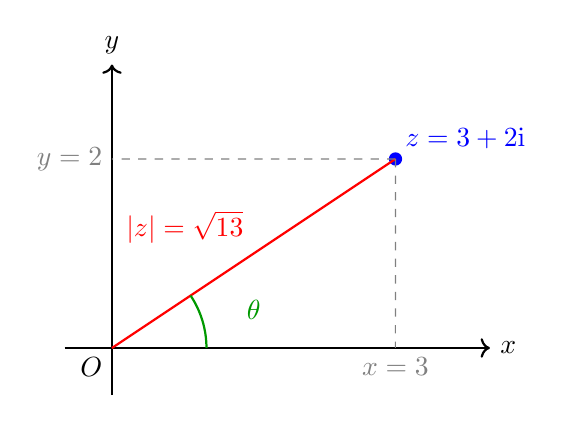
\begin{tikzpicture}[scale=1.2]
    % 坐标轴
    \draw[->, thick] (-0.5, 0) -- (4, 0) node[right] {$x$};
    \draw[->, thick] (0, -0.5) -- (0, 3) node[above] {$y$};
    
    % 复数\index{复数} z = 3 + 2i
    \coordinate (z) at (3, 2);
    \fill[blue] (z) circle (2pt) node[above right] {$z = 3 + 2\mathrm{i}$};
    
    % 模
    \draw[thick, red] (0, 0) -- (z) node[midway, above left] {$|z| = \sqrt{13}$};
    
    % 辐角
    \draw[thick, green!60!black] (1, 0) arc (0:33.69:1);
    \node[green!60!black] at (1.5, 0.4) {$\theta$};
    
    % 坐标分量
    \draw[dashed, gray] (z) -- (3, 0) node[below] {$x=3$};
    \draw[dashed, gray] (z) -- (0, 2) node[left] {$y=2$};
    
    \node[below left] at (0, 0) {$O$};
\end{tikzpicture}
\caption{复数\index{复数}的模与辐角}
\label{fig:modulus-argument}
\end{figure}

\begin{lizi}{}{}
计算复数\index{复数} $z = 3 + 2\mathrm{i}$ 的模。
\begin{jie}
    $|z| = \sqrt{3^2 + 2^2} = \sqrt{9 + 4} = \sqrt{13}$
\end{jie}
\end{lizi}

\subsection{复数\index{复数}的辐角}

复数\index{复数} $z \neq 0$ 的\textbf{辐角} $\theta$ 是实轴正方向到向量 $\overrightarrow{Oz}$ 的夹角：
\begin{equation}
    \tan\theta = \frac{y}{x}
\end{equation}
辐角有无穷多个值，相差 $2\pi$ 的整数倍。满足 $-\pi < \theta \leq \pi$ 的辐角称为\textbf{主辐角}，记作 $\operatorname{Arg}(z)$，而全体辐角记作 $\arg(z) = \operatorname{Arg}(z) + 2k\pi$（$k \in \mathbb{Z}$）。

\begin{jinshi}[常见错误：直接用反正切]
计算辐角时，不能简单地用 $\theta = \arctan(y/x)$，因为反正切函数的值域是 $(-\pi/2, \pi/2)$，无法区分第二、三象限的点。

正确的做法是：
\begin{itemize}
    \item 先根据 $x, y$ 的符号确定象限。
    \item 再用 $\arctan$ 计算参考角。
\end{itemize}
\end{jinshi}

\begin{lizi}{}{}
求复数\index{复数} $z = -1 - \mathrm{i}$ 的模和主辐角。
\begin{jie}
    模：$|z| = \sqrt{(-1)^2 + (-1)^2} = \sqrt{2}$

    主辐角：点 $(-1, -1)$ 在第三象限。$\arctan(1) = \pi/4$，所以主辐角为 $-\pi + \pi/4 = -3\pi/4$。
\end{jie}
\end{lizi}

\subsection{复数\index{复数}的三角形式与指数形式}

利用模和辐角，复数\index{复数}可以表示为\textbf{三角形式}：
\begin{equation}
    z = |z|(\cos\theta + \mathrm{i}\sin\theta) = r(\cos\theta + \mathrm{i}\sin\theta)
\end{equation}
其中 $r = |z|$，$\theta$ 是辐角。

利用\keyword{欧拉公式}（下一章证明）：
\begin{zhongyao}[欧拉公式]
    $\mathrm{e}^{\mathrm{i}\theta} = \cos\theta + \mathrm{i}\sin\theta$
\end{zhongyao}
复数\index{复数}还可以写成\textbf{指数形式}（或\textbf{极坐标形式}）：
\begin{equation}
    z = r\mathrm{e}^{\mathrm{i}\theta}
\end{equation}

\begin{tishi}[三种形式的选择]
\begin{itemize}
    \item \textbf{代数形式} $z = x + \mathrm{i}y$：适合加法、减法。
    \item \textbf{三角形式} $z = r(\cos\theta + \mathrm{i}\sin\theta)$：适合推导公式。
    \item \textbf{指数形式} $z = r\mathrm{e}^{\mathrm{i}\theta}$：适合乘法、除法、幂运算。
\end{itemize}
解题时根据运算类型选择合适的形式。
\end{tishi}

\subsection{共轭复数\index{复数}}

复数\index{复数} $z = x + \mathrm{i}y$ 的\textbf{共轭复数\index{复数}}定义为
\begin{equation}
    \bar{z} = x - \mathrm{i}y
\end{equation}
即把虚部取相反数。

几何上，共轭复数\index{复数} $\bar{z}$ 关于实轴与 $z$ 对称。

\begin{figure}[htbp]
\centering
\begin{tikzpicture}[scale=1.2]
    % 坐标轴
    \draw[->, thick] (-0.5, 0) -- (4, 0) node[right] {$x$};
    \draw[->, thick] (0, -2.5) -- (0, 2.5) node[above] {$y$};
    
    % 复数\index{复数} z
    \coordinate (z) at (3, 2);
    \fill[blue] (z) circle (2pt) node[above right] {$z = 3 + 2\mathrm{i}$};
    
    % 共轭复数\index{复数}
    \coordinate (zbar) at (3, -2);
    \fill[red] (zbar) circle (2pt) node[below right] {$\bar{z} = 3 - 2\mathrm{i}$};
    
    % 对称线
    \draw[dashed, gray] (z) -- (zbar);
    
    \node[below left] at (0, 0) {$O$};
\end{tikzpicture}
\caption{共轭复数\index{复数}的几何意义}
\label{fig:conjugate}
\end{figure}

共轭复数\index{复数}有以下重要性质：

\begin{dingli}{}{共轭复数的性质}
设 $z = x + \mathrm{i}y$，则：
\begin{enumerate}
    \item $z + \bar{z} = 2x = 2\operatorname{Re}(z)$
    \item $z - \bar{z} = 2\mathrm{i}y = 2\mathrm{i}\operatorname{Im}(z)$
    \item $z\bar{z} = |z|^2 = x^2 + y^2$
    \item $\overline{z_1 + z_2} = \bar{z}_1 + \bar{z}_2$
    \item $\overline{z_1 z_2} = \bar{z}_1 \bar{z}_2$
    \item $\overline{z^n} = (\bar{z})^n$
    \item $|\bar{z}| = |z|$
    \item $\arg(\bar{z}) = -\arg(z)$
\end{enumerate}
\end{dingli}

\begin{proof}
我们证明第3条性质，其余留给读者。

设 $z = x + \mathrm{i}y$，则 $\bar{z} = x - \mathrm{i}y$。
\begin{align}
    z\bar{z} &= (x + \mathrm{i}y)(x - \mathrm{i}y) \\
             &= x^2 - \mathrm{i}xy + \mathrm{i}xy - \mathrm{i}^2 y^2 \\
             &= x^2 + y^2 = |z|^2
\end{align}
\end{proof}

\begin{lizi}{}{}
利用共轭复数\index{复数}计算 $\displaystyle\frac{3 + 2\mathrm{i}}{1 - \mathrm{i}}$。
\begin{jie}
    将分母``实数化''：分子分母同乘分母的共轭复数\index{复数}。
    \begin{align}
        \frac{3 + 2\mathrm{i}}{1 - \mathrm{i}} &= \frac{(3 + 2\mathrm{i})(1 + \mathrm{i})}{(1 - \mathrm{i})(1 + \mathrm{i})} \\
        &= \frac{3 + 3\mathrm{i} + 2\mathrm{i} + 2\mathrm{i}^2}{1 - \mathrm{i}^2} \\
        &= \frac{3 + 5\mathrm{i} - 2}{2} \\
        &= \frac{1 + 5\mathrm{i}}{2} = \frac{1}{2} + \frac{5}{2}\mathrm{i}
    \end{align}
\end{jie}
\end{lizi}

% ========== 第三节 ==========
\section{复数\index{复数}的运算与几何意义}

\subsection{加法与减法}

\begin{dingliyi}{}{复数的加减}
设 $z_1 = x_1 + \mathrm{i}y_1$，$z_2 = x_2 + \mathrm{i}y_2$，则
\begin{align}
    z_1 + z_2 &= (x_1 + x_2) + \mathrm{i}(y_1 + y_2) \\
    z_1 - z_2 &= (x_1 - x_2) + \mathrm{i}(y_1 - y_2)
\end{align}
\end{dingliyi}

\textbf{几何意义}：复数\index{复数}加法对应向量加法（平行四边形法则或三角形法则），减法对应向量减法。

\begin{figure}[htbp]
\centering
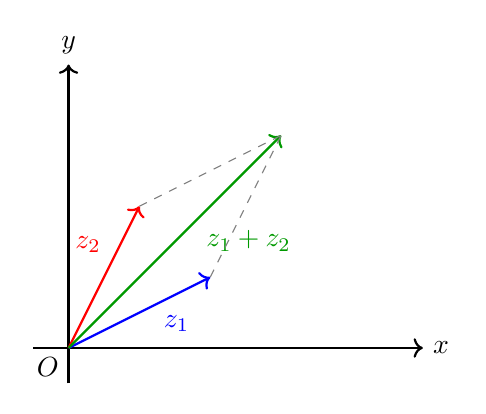
\begin{tikzpicture}[scale=0.9]
    % 坐标轴
    \draw[->, thick] (-0.5, 0) -- (5, 0) node[right] {$x$};
    \draw[->, thick] (0, -0.5) -- (0, 4) node[above] {$y$};
    
    % 向量 z1, z2
    \coordinate (z1) at (2, 1);
    \coordinate (z2) at (1, 2);
    \coordinate (zsum) at (3, 3);
    
    \draw[->, thick, blue] (0, 0) -- (z1) node[pos=0.6, below right] {$z_1$};
    \draw[->, thick, red] (0, 0) -- (z2) node[pos=0.6, above left] {$z_2$};
    \draw[->, thick, green!60!black] (0, 0) -- (zsum) node[pos=0.6, below right] {$z_1+z_2$};
    
    % 平行四边形
    \draw[dashed, gray] (z1) -- (zsum);
    \draw[dashed, gray] (z2) -- (zsum);
    
    \node[below left] at (0, 0) {$O$};
\end{tikzpicture}
\caption{复数\index{复数}加法的平行四边形法则}
\label{fig:complex-add}
\end{figure}

\subsection{乘法}

\begin{dingliyi}{}{复数的乘法}
设 $z_1 = x_1 + \mathrm{i}y_1$，$z_2 = x_2 + \mathrm{i}y_2$，则
\begin{equation}
    z_1 z_2 = (x_1 x_2 - y_1 y_2) + \mathrm{i}(x_1 y_2 + x_2 y_1)
\end{equation}
\end{dingliyi}

这个公式不太好记。如果用指数形式，就简单多了：

设 $z_1 = r_1 \mathrm{e}^{\mathrm{i}\theta_1}$，$z_2 = r_2 \mathrm{e}^{\mathrm{i}\theta_2}$，则
\begin{equation}
    z_1 z_2 = r_1 r_2 \mathrm{e}^{\mathrm{i}(\theta_1 + \theta_2)}
\end{equation}

\textbf{几何意义}：两个复数相乘，模相乘，辐角相加。这意味着：
\begin{itemize}
    \item \keyword{模}乘以 $r_2$：向量的长度伸缩 $r_2$ 倍。
    \item \keyword{辐角}加 $\theta_2$：向量逆时针旋转 $\theta_2$ 角。
\end{itemize}

\begin{figure}[htbp]
\centering
\begin{tikzpicture}[scale=0.85]
    % z 平面
    \begin{scope}
        \draw[->, thick, gray] (-0.5, 0) -- (4.5, 0) node[right] {$x$};
        \draw[->, thick, gray] (0, -0.5) -- (0, 3.5) node[above] {$y$};
        
        % z1
        \coordinate (z1) at (2, 1);
        \draw[->, very thick, blue] (0, 0) -- (z1);
        \fill[blue] (z1) circle (2pt) node[above right] {$z_1$};
        \draw[blue, dashed] (0, 0) -- (2, 0) node[below] {$r_1$};
        \draw[blue, thick] (0.6, 0) arc (0:26.57:0.6);
        \node[blue] at (0.9, 0.25) {$\theta_1$};
        
        % z2
        \coordinate (z2) at (1, 2.5);
        \draw[->, very thick, red] (0, 0) -- (z2);
        \fill[red] (z2) circle (2pt) node[above] {$z_2$};
        \draw[red, thick] (0.4, 0) arc (0:68.2:0.4);
        \node[red] at (0.5, 0.6) {$\theta_2$};
        
        \node at (2, -1) {$z$ 平面};
    \end{scope}
    
    % 箭头
    \draw[->, very thick, purple!70!black] (5, 1.5) -- (6.5, 1.5) node[midway, above] {$\times z_2$};
    
    % w 平面
    \begin{scope}[xshift=8cm]
        \draw[->, thick, gray] (-0.5, 0) -- (5, 0) node[right] {$x$};
        \draw[->, thick, gray] (0, -0.5) -- (0, 4.5) node[above] {$y$};
        
        % z1*z2 (模变大，角度增加)
        \coordinate (prod) at (2.5, 4);
        \draw[->, very thick, purple!70!black] (0, 0) -- (prod);
        \fill[purple!70!black] (prod) circle (2pt) node[above right] {$z_1 z_2$};
        
        % 原来的z1（虚线）
        \draw[dashed, blue!50] (0, 0) -- (2, 1);
        
        % 模标注
        \draw[purple!70!black, dashed] (0, 0) -- (2.5, 0) node[below] {$r_1 r_2$};
        \draw[purple!70!black, thick] (0.8, 0) arc (0:58:0.8);
        \node[purple!70!black] at (1.3, 0.7) {$\theta_1+\theta_2$};
        
        \node at (2.5, -1) {$w$ 平面};
    \end{scope}
\end{tikzpicture}
\caption{复数乘法的几何意义：模伸缩、辐角相加}
\label{fig:complex-mult}
\end{figure}

\begin{tishi}[乘以 $\mathrm{i}$ 的几何意义]
$\mathrm{i} = \mathrm{e}^{\mathrm{i}\pi/2}$，模为 $1$，辐角为 $\pi/2$（即 $90°$）。因此，任何复数 $z$ 乘以 $\mathrm{i}$，相当于：
\begin{itemize}
    \item 模不变（$|\mathrm{i}| = 1$）
    \item 辐角增加 $90°$，即逆时针旋转 $90°$
\end{itemize}
这正是为什么 $\mathrm{i}$ 在交流电路中代表 $90°$ 相位差的原因。
\end{tishi}

\begin{wulibj}[复数乘法与旋转矩阵]
复数乘法与二维旋转矩阵有深刻的对应关系。

设 $z_2 = \cos\theta + \mathrm{i}\sin\theta$（模为 $1$ 的复数），则 $z_1 \cdot z_2$ 相当于把 $z_1$ 旋转 $\theta$ 角。

用代数形式展开：设 $z_1 = x + \mathrm{i}y$，$z_2 = \cos\theta + \mathrm{i}\sin\theta$，则
\begin{align}
    z_1 z_2 &= (x + \mathrm{i}y)(\cos\theta + \mathrm{i}\sin\theta) \notag \\
           &= (x\cos\theta - y\sin\theta) + \mathrm{i}(x\sin\theta + y\cos\theta)
\end{align}
这与二维旋转矩阵的作用完全一致：
\begin{equation}
    \begin{pmatrix} x' \\ y' \end{pmatrix} = 
    \begin{pmatrix} \cos\theta & -\sin\theta \\ \sin\theta & \cos\theta \end{pmatrix}
    \begin{pmatrix} x \\ y \end{pmatrix}
\end{equation}
也就是说：\textbf{复数乘法等价于二维平面上的旋转变换}（当模为 $1$ 时）或旋转加缩放变换（一般情况）。这个对应关系在计算机图形学、机器人学中有广泛应用。
\end{wulibj}

\begin{lizi}{}{}
设 $z = 1 + \mathrm{i}$，求 $z^4$。
\begin{jie}
    先化成指数形式。$|z| = \sqrt{2}$，$\theta = \pi/4$，所以
    \begin{equation}
        z = \sqrt{2}\,\mathrm{e}^{\mathrm{i}\pi/4}
    \end{equation}
    于是
    \begin{equation}
        z^4 = (\sqrt{2})^4 \mathrm{e}^{\mathrm{i}\pi} = 4(-1) = -4
    \end{equation}
\end{jie}
\end{lizi}

\subsection{除法}

\begin{dingliyi}{}{复数的除法}
设 $z_1 = x_1 + \mathrm{i}y_1$，$z_2 = x_2 + \mathrm{i}y_2 \neq 0$，则
\begin{equation}
    \frac{z_1}{z_2} = \frac{z_1 \bar{z}_2}{|z_2|^2} = \frac{(x_1 x_2 + y_1 y_2) + \mathrm{i}(x_2 y_1 - x_1 y_2)}{x_2^2 + y_2^2}
\end{equation}
\end{dingliyi}

用指数形式更简洁：若 $z_1 = r_1 \mathrm{e}^{\mathrm{i}\theta_1}$，$z_2 = r_2 \mathrm{e}^{\mathrm{i}\theta_2}$，则
\begin{equation}
    \frac{z_1}{z_2} = \frac{r_1}{r_2} \mathrm{e}^{\mathrm{i}(\theta_1 - \theta_2)}
\end{equation}

\textbf{几何意义}：模相除，辐角相减。

\subsection{乘方与开方}

\subsubsection{乘方}

设 $z = r\mathrm{e}^{\mathrm{i}\theta}$，则 $z$ 的 $n$ 次幂为
\begin{equation}
    z^n = r^n \mathrm{e}^{\mathrm{i}n\theta}
\end{equation}

特别地，当 $r = 1$ 时，有\textbf{棣莫弗公式}：
\begin{equation}
    (\cos\theta + \mathrm{i}\sin\theta)^n = \cos n\theta + \mathrm{i}\sin n\theta
\end{equation}
\begin{lizi}{}{}
用棣莫弗公式计算 $\cos 3\theta$。
\begin{jie}
    由棣莫弗公式：
    \begin{align}
        \cos 3\theta + \mathrm{i}\sin 3\theta &= (\cos\theta + \mathrm{i}\sin\theta)^3 \\
        &= \cos^3\theta + 3\mathrm{i}\cos^2\theta\sin\theta - 3\cos\theta\sin^2\theta - \mathrm{i}\sin^3\theta
    \end{align}
    比较实部，得
    \begin{equation}
        \cos 3\theta = \cos^3\theta - 3\cos\theta\sin^2\theta = 4\cos^3\theta - 3\cos\theta
    \end{equation}
\end{jie}
\end{lizi}

\subsubsection{开方}

设 $z = r\mathrm{e}^{\mathrm{i}\theta}$，求 $z$ 的 $n$ 次方根 $w = \sqrt[n]{z}$。

设 $w = \rho\mathrm{e}^{\mathrm{i}\varphi}$，则 $w^n = z$ 给出
\begin{equation}
    \rho^n \mathrm{e}^{\mathrm{i}n\varphi} = r\mathrm{e}^{\mathrm{i}\theta}
\end{equation}
因此 $\rho = \sqrt[n]{r}$，$n\varphi = \theta + 2k\pi$（$k = 0, 1, \ldots, n-1$），即
\begin{equation}
    \varphi_k = \frac{\theta + 2k\pi}{n}, \quad k = 0, 1, \ldots, n-1
\end{equation}

所以 $z$ 的 $n$ 次方根有 $n$ 个值：
\begin{equation}
    w_k = \sqrt[n]{r} \, \mathrm{e}^{\mathrm{i}(\theta + 2k\pi)/n}, \quad k = 0, 1, \ldots, n-1
\end{equation}

\begin{tishi}[几何意义]
$n$ 次方根的 $n$ 个值均匀分布在以原点为圆心、$\sqrt[n]{|z|}$ 为半径的圆周上，构成一个正 $n$ 边形。
\end{tishi}

\begin{figure}[htbp]
\centering
\begin{tikzpicture}[scale=1.5]
    % 圆
    \draw[gray, dashed] (0,0) circle (1);
    
    % 坐标轴
    \draw[->, thick] (-1.5, 0) -- (1.5, 0) node[right] {$x$};
    \draw[->, thick] (0, -1.5) -- (0, 1.5) node[above] {$y$};
    
    % 单位根
    \foreach \k in {0,1,2,3,4,5} {
        \pgfmathsetmacro{\angle}{60*\k}
        \coordinate (w\k) at (\angle:1);
        \fill[blue] (w\k) circle (1.5pt);
        \node at (\angle:1.25) {$w_{\k}$};
    }
    
    % 连接成正六边形
    \draw[blue!50, thick] (w0) -- (w1) -- (w2) -- (w3) -- (w4) -- (w5) -- cycle;
    
    \node[below] at (0, -1.8) {$1$ 的 $6$ 次方根};
\end{tikzpicture}
\caption{$1$ 的 $n$ 次方根构成正 $n$ 边形}
\label{fig:roots-unity}
\end{figure}

\begin{lizi}{}{}
求 $z = 1$ 的立方根。
\begin{jie}
    写成指数形式：$z = 1 = \mathrm{e}^{\mathrm{i}\cdot 0}$。
    
    立方根为
    \begin{equation}
        w_k = \mathrm{e}^{\mathrm{i} \cdot 2k\pi/3}, \quad k = 0, 1, 2
    \end{equation}
    
    即
    \begin{align}
        w_0 &= \mathrm{e}^0 = 1 \\
        w_1 &= \mathrm{e}^{\mathrm{i}2\pi/3} = -\frac{1}{2} + \frac{\sqrt{3}}{2}\mathrm{i} \\
        w_2 &= \mathrm{e}^{\mathrm{i}4\pi/3} = -\frac{1}{2} - \frac{\sqrt{3}}{2}\mathrm{i}
    \end{align}
    
    这三个值在复平面上构成正三角形。
\end{jie}
\end{lizi}

% ========== 第四节 ==========
\section{复平面上的点集：区域、曲线、连通性}

在研究复变函数之前，我们需要先了解复平面上的一些基本概念。这些概念是后续讨论函数定义域、积分路径等的基础。

\subsection{点的邻域}

\begin{dingliyi}{}{邻域}
设 $z_0$ 是复平面上的一个点，$\varepsilon > 0$ 是正数。点集
\begin{equation}
    U(z_0, \varepsilon) = \{z \in \mathbb{C} : |z - z_0| < \varepsilon\}
\end{equation}
称为点 $z_0$ 的\textbf{$\varepsilon$ 邻域}，即以 $z_0$ 为圆心、$\varepsilon$ 为半径的开圆盘。
\end{dingliyi}

\begin{figure}[htbp]
\centering
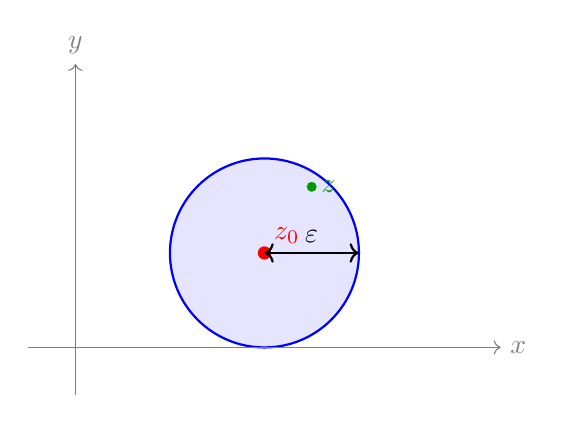
\begin{tikzpicture}[scale=1.2]
    % 圆
    \draw[blue, thick, fill=blue!10] (2, 1) circle (1);
    
    % 圆心
    \fill[red] (2, 1) circle (2pt) node[above right] {$z_0$};
    
    % 半径
    \draw[<->, thick] (2, 1) -- (3, 1) node[midway, above] {$\varepsilon$};
    
    % 任意点
    \fill[green!60!black] (2.5, 1.7) circle (1.5pt) node[right] {$z$};
    
    % 坐标轴
    \draw[->, gray] (-0.5, 0) -- (4.5, 0) node[right] {$x$};
    \draw[->, gray] (0, -0.5) -- (0, 3) node[above] {$y$};
\end{tikzpicture}
\caption{点 $z_0$ 的 $\varepsilon$ 邻域}
\label{fig:neighborhood}
\end{figure}

\subsection{内点、外点、边界点}

\begin{dingliyi}{}{内点、外点、边界点}
设 $E$ 是复平面上的一个点集，$z_0$ 是一个点。
\begin{itemize}
    \item 若存在 $\varepsilon > 0$，使得 $U(z_0, \varepsilon) \subset E$，则称 $z_0$ 是 $E$ 的\textbf{内点}。
    \item 若存在 $\varepsilon > 0$，使得 $U(z_0, \varepsilon) \cap E = \emptyset$，则称 $z_0$ 是 $E$ 的\textbf{外点}。
    \item 若 $z_0$ 既不是 $E$ 的内点也不是外点，即 $z_0$ 的任意邻域内既有 $E$ 中的点又有不在 $E$ 中的点，则称 $z_0$ 是 $E$ 的\textbf{边界点}。
\end{itemize}
\end{dingliyi}

\begin{lizi}{}{}
    设 $E = \{z : |z| < 1\}$ 是单位开圆盘。判断以下点的类型：
    \begin{enumerate}
        \item $z_1 = 0$
        \item $z_2 = 1$
        \item $z_3 = 2$
    \end{enumerate}
    \begin{jie}
        \begin{enumerate}
            \item $z_1 = 0$：内点。因为存在邻域 $U(0, 0.5) \subset E$，完全在 $E$ 内。
            \item $z_2 = 1$：边界点。任意邻域 $U(1, \varepsilon)$ 内既有 $E$ 中的点（如 $1 - \varepsilon/2$），又有 $E$ 外的点（如 $1 + \varepsilon/2$）。
            \item $z_3 = 2$：外点。存在邻域 $U(2, 0.5)$ 与 $E$ 不相交。
        \end{enumerate}
    \end{jie}
\end{lizi}

\subsection{开集与闭集}

\begin{dingliyi}{}{开集与闭集}
\begin{itemize}
    \item 若点集 $E$ 中的每个点都是内点，则称 $E$ 是\textbf{开集}。
    \item 若点集 $E$ 的补集 $\mathbb{C} \setminus E$ 是开集，则称 $E$ 是\textbf{闭集}。
    \item 点集 $E$ 的所有边界点构成的集合称为 $E$ 的\textbf{边界}，记作 $\partial E$。
\end{itemize}
\end{dingliyi}

\begin{zhu}{}{}
``开''和``闭''不是互斥的。例如，空集 $\emptyset$ 和全空间 $\mathbb{C}$ 既开又闭。
\end{zhu}

\subsection{区域}

\begin{dingliyi}{}{区域}
若点集 $D$ 满足：
\begin{enumerate}
    \item $D$ 是开集；
    \item $D$ 是连通的，即 $D$ 中任意两点都可以用一条完全在 $D$ 内的曲线连接。
\end{enumerate}
则称 $D$ 是一个\textbf{区域}。

区域 $D$ 连同它的边界 $\partial D$ 构成的集合称为\textbf{闭区域}，记作 $\bar{D} = D \cup \partial D$。
\end{dingliyi}

\begin{figure}[htbp]
\centering
\begin{tikzpicture}[scale=0.8]
    % 左图：区域
    \begin{scope}
        \draw[blue, thick, fill=blue!20] (0, 0) circle (1.5);
        \draw[blue, thick, fill=blue!20] (2.5, 0) circle (1);
        % 连接部分
        \draw[blue, thick, fill=blue!20] (0, 0) -- (2.5, 0);
        
        \node at (1.25, -2.5) {(a) 区域（连通开集）};
    \end{scope}
    
    % 右图：非区域
    \begin{scope}[xshift=7cm]
        \draw[blue, thick, fill=blue!20] (0, 0) circle (1.5);
        \draw[blue, thick, fill=blue!20] (3, 0) circle (1);
        % 不连接
        
        \node at (1.5, -2.5) {(b) 非区域（不连通）};
    \end{scope}
\end{tikzpicture}
\caption{区域与非区域的区别}
\label{fig:region}
\end{figure}

\subsection{单连通与多连通区域}

\begin{dingliyi}{}{单连通区域}
若区域 $D$ 内任意一条简单闭曲线的内部仍在 $D$ 内，则称 $D$ 是\textbf{单连通区域}。否则称为\textbf{多连通区域}。

直观地说，单连通区域是``没有洞''的区域。
\end{dingliyi}

\begin{figure}[htbp]
\centering
\begin{tikzpicture}[scale=0.9]
    % 单连通
    \begin{scope}
        \draw[blue, thick, fill=blue!20] (0, 0) ellipse (1.5 and 1);
        \node at (0, -2) {(a) 单连通区域};
        
        % 闭曲线
        \draw[red, thick, dashed] (0, 0) circle (0.5);
        \node[red] at (0, 0.8) {\small 闭曲线};
    \end{scope}
    
    % 多连通
    \begin{scope}[xshift=5cm]
        \draw[blue, thick, fill=blue!20] (0, 0) ellipse (1.5 and 1);
        \draw[white, thick, fill=white] (0, 0) circle (0.4);
        \draw[blue, thick] (0, 0) circle (0.4);
        \node at (0, -2) {(b) 多连通区域（有洞）};
        
        % 闭曲线
        \draw[red, thick, dashed] (0, 0) circle (0.25);
    \end{scope}
    
    % 环形区域
    \begin{scope}[xshift=10cm]
        \draw[blue, thick, fill=blue!20] (0, 0) circle (1.5);
        \draw[white, thick, fill=white] (0, 0) circle (0.5);
        \draw[blue, thick] (0, 0) circle (0.5);
        \node at (0, -2) {(c) 环形区域（多连通）};
    \end{scope}
\end{tikzpicture}
\caption{单连通与多连通区域}
\label{fig:simply-connected}
\end{figure}

\begin{zhu}{}{}
单连通与多连通的区别在研究柯西积分定理\index{柯西积分定理}时非常重要。简单来说：
\begin{itemize}
    \item 在单连通区域内，闭路积分可以``收缩''为一点。
    \item 在多连通区域内，围绕``洞''的闭路积分可能不为零。
\end{itemize}
\end{zhu}

% ========== 第五节 ==========
\section{复球面与扩充复平面}

到目前为止，我们用平面上的点来表示复数。但当我们讨论无穷远点时，平面表示会遇到困难——无穷远点在哪里？为了解决这个问题，我们引入复球面（黎曼球面）的概念。

\subsection{球极投影}

考虑一个单位球面，放在复平面上方，使得球的南极与原点相切。设球的北极为 $N$，南极为 $S$。

\begin{dingliyi}{}{球极投影}
对于复平面上任意一点 $z$，连接 $N$ 和 $z$ 的直线与球面相交于一点 $P$（异于 $N$）。这个映射 $z \mapsto P$ 称为\textbf{球极投影}。
\end{dingliyi}

\begin{figure}[htbp]
\centering
\begin{tikzpicture}[scale=1.0]
    % 球面
    \shade[ball color=blue!20, opacity=0.6] (0, 0) circle (1.5);
    \draw[thick] (0, 0) circle (1.5);
    
    % 坐标轴（复平面）
    \draw[->, thick] (-3, -1.5) -- (3, -1.5) node[right] {$x$};
    \draw[->, thick] (0, -1.5) -- (0, 2.5) node[above] {$y$};
    
    % 复平面上的点
    \coordinate (z) at (2, -1.5);
    \fill[red] (z) circle (2pt) node[below] {$z$};
    
    % 北极
    \coordinate (N) at (0, 1.5);
    \fill[blue] (N) circle (2pt) node[above right] {$N$};
    
    % 南极
    \coordinate (S) at (0, -1.5);
    \fill[green!60!black] (S) circle (2pt) node[below] {$S$ (原点)};
    
    % 球面上的点 P
    \coordinate (P) at (1.2, 0.6);
    \fill[orange] (P) circle (2pt) node[right] {$P$};
    
    % 投影线
    \draw[dashed, thick, purple] (N) -- (z);
    
    % 标注
    \node at (0, -2.5) {复平面};
    \node at (2.2, 2) {球面};
\end{tikzpicture}
\caption{球极投影：复平面上的点 $z$ 映射到球面上的点 $P$}
\label{fig:stereographic}
\end{figure}

通过球极投影，复平面上的每一点都唯一对应球面上的一个点（除北极 $N$ 外）。

\subsection{无穷远点}

当复平面上的点 $z$ 越来越远离原点（即 $|z| \to \infty$）时，投影点 $P$ 会越来越接近北极 $N$。

\begin{dingliyi}{}{无穷远点}
在球极投影下，北极 $N$ 对应复平面上的一个特殊的点，称为\textbf{无穷远点}，记作 $\infty$。
\end{dingliyi}

引入无穷远点后，复平面被扩充为\textbf{扩充复平面}（或\textbf{闭复平面}）：
\begin{equation}
    \overline{\mathbb{C}} = \mathbb{C} \cup \{\infty\}
\end{equation}

\begin{tishi}[无穷远点的直观理解]
无穷远点 $\infty$ 可以理解为：
\begin{itemize}
    \item 模 $|z|$ 趋于无穷大的点的极限位置
    \item 不论从哪个方向趋向无穷，最终都到达同一个点 $\infty$
    \item 在复球面上，$\infty$ 就是北极 $N$
\end{itemize}
这与实数中的 $+\infty$ 和 $-\infty$ 不同——复平面中只有一个无穷远点。
\end{tishi}

\subsection{无穷远点的运算}

对于无穷远点，我们可以定义一些合理的运算：

\begin{dingliyi}{}{无穷远点的运算规则}
设 $z \in \mathbb{C}$ 是有限复数，$z \neq 0$。约定：
\begin{align}
    z + \infty &= \infty + z = \infty \\
    z \cdot \infty &= \infty \cdot z = \infty \quad (z \neq 0) \\
    \frac{z}{0} &= \infty \quad (z \neq 0) \\
    \frac{z}{\infty} &= 0 \\
    \frac{\infty}{z} &= \infty \quad (z \neq 0)
\end{align}
\end{dingliyi}

\begin{jinshi}[无定义的运算]
以下运算在扩充复平面中仍然无定义：
\begin{itemize}
    \item $\infty + \infty$
    \item $\infty - \infty$
    \item $\infty \cdot 0$ 和 $0 \cdot \infty$
    \item $\frac{\infty}{\infty}$
    \item $\frac{0}{0}$
\end{itemize}
这些都是不定式，需要具体情况具体分析。
\end{jinshi}

\subsection{扩充复平面的拓扑}

在扩充复平面 $\overline{\mathbb{C}}$ 上，无穷远点 $\infty$ 也有它的邻域：

\begin{dingliyi}{}{无穷远点的邻域}
点集
\begin{equation}
    U(\infty, R) = \{z \in \mathbb{C} : |z| > R\} \cup \{\infty\}
\end{equation}
称为无穷远点的\textbf{$R$ 邻域}，即复平面上圆 $|z| = R$ 外部的区域加上 $\infty$。
\end{dingliyi}

\begin{figure}[htbp]
\centering
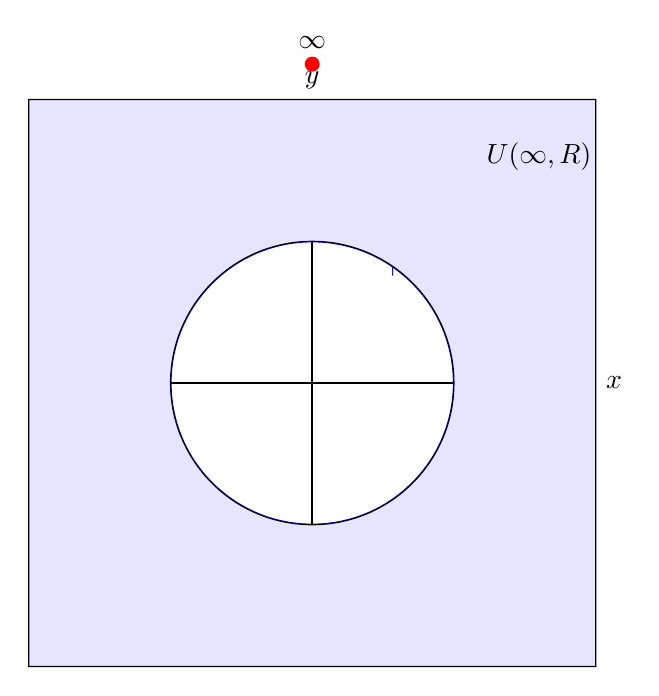
\begin{tikzpicture}[scale=0.9]
    % 坐标轴
    \draw[->, thick] (-4, 0) -- (4, 0) node[right] {$x$};
    \draw[->, thick] (0, -4) -- (0, 4) node[above] {$y$};
    
    % 圆
    \draw[blue, thick] (0, 0) circle (2);
    \node[blue] at (1.7, 1.7) {$|z| = R$};
    
    % 外部区域（阴影）
    \draw[fill=blue!10, even odd rule] (-4, -4) rectangle (4, 4) (0, 0) circle (2);
    
    % 无穷远点
    \node at (0, 4.8) {$\infty$};
    \fill[red] (0, 4.5) circle (3pt);
    
    % 标注
    \node at (3.2, 3.2) {$U(\infty, R)$};
\end{tikzpicture}
\caption{无穷远点的邻域：圆外区域}
\label{fig:infinity-neighborhood}
\end{figure}

\begin{wulibj}[复球面的好处]
复球面提供了一个完美的拓扑图景：
\begin{enumerate}
    \item \textbf{紧致性}：$\overline{\mathbb{C}}$ 是紧致的（类似于闭区间 $[a, b]$），而 $\mathbb{C}$ 不是。这意味着在 $\overline{\mathbb{C}}$ 上，任何无穷点列都有收敛子列。
    \item \textbf{统一性}：无穷远点和有限点地位平等，都是球面上的普通点。
    \item \textbf{留数理论}：我们可以定义无穷远点的留数，使留数定理更完整。
    \item \textbf{保角映射}：奇点的分类和讨论更方便。
\end{enumerate}
\end{wulibj}

\begin{lizi}{}{}
在扩充复平面上，圆 $|z| = 1$ 把平面分成两部分：内部和外部。问这两部分在复球面上分别是什么形状？
 \begin{jie}
    在复球面上：
    \begin{itemize}
        \item 圆的内部 $|z| < 1$ 映射为球面上靠近南极的球冠。
        \item 圆的外部 $|z| > 1$（连同 $\infty$）映射为球面上靠近北极的球冠。
        \item 圆周 $|z| = 1$ 映射为球面上的纬线圈。
    \end{itemize}
    所以，一个圆把球面分成两个球冠，地位是平等的。
 \end{jie}
\end{lizi}

\subsection{复球面上的直线与圆}

在复球面上，直线和圆有统一的观点。

\begin{dingli}{}{扩充复平面上的圆}
在扩充复平面上，\textbf{圆}是满足方程
\begin{equation}
    A|z|^2 + \bar{B}z + B\bar{z} + C = 0
\end{equation}
的点集，其中 $A, C \in \mathbb{R}$，$B \in \mathbb{C}$，且 $|B|^2 > AC$（保证曲线非退化）。

特别地：
\begin{itemize}
    \item 当 $A \neq 0$ 时，是普通圆（圆心 $-B/A$，半径 $\sqrt{|B|^2 - AC}/|A|$）。
    \item 当 $A = 0$ 时，是直线（过无穷远点）。
\end{itemize}
\end{dingli}

这个统一观点在研究保角映射时非常有用——保角映射把圆变成圆（广义的，包括直线）。

% ========== 第六节 ==========
\section{复数\index{复数}的应用：交流电路、量子力学}

前面我们学习了复数\index{复数}的基本概念和运算。现在让我们看看复数\index{复数}在物理中的两个重要应用。

\subsection{交流电路中的复数\index{复数}方法}

在交流电路中，电压和电流都是时间的正弦函数。直接用三角函数进行运算非常繁琐，而用复数\index{复数}表示则可以大大简化计算。

\subsubsection{相量表示}

设电压和电流为
\begin{align}
    u(t) &= U_0 \cos(\omega t + \varphi_u) \\
    i(t) &= I_0 \cos(\omega t + \varphi_i)
\end{align}
其中 $U_0$、$I_0$ 是振幅，$\omega$ 是角频率，$\varphi_u$、$\varphi_i$ 是初相位。

引入\textbf{相量}（复数\index{复数}）表示：
\begin{align}
    \dot{U} &= U_0 \mathrm{e}^{\mathrm{i}\varphi_u} \\
    \dot{I} &= I_0 \mathrm{e}^{\mathrm{i}\varphi_i}
\end{align}

注意：相量只包含振幅和相位信息，不包含频率。同一频率的交流量才能用相量运算。

\subsubsection{阻抗的复数\index{复数}表示}

对于电阻 $R$、电感 $L$、电容 $C$，定义\textbf{复阻抗}：
\begin{align}
    Z_R &= R \\
    Z_L &= \mathrm{i}\omega L \\
    Z_C &= \frac{1}{\mathrm{i}\omega C} = -\frac{\mathrm{i}}{\omega C}
\end{align}

\begin{tishi}[为什么电感阻抗有 $\mathrm{i}$？]
电感两端的电压 $u = L \frac{\mathrm{d}i}{\mathrm{d}t}$。若 $i = I_0 \cos(\omega t)$，则
\begin{equation}
    u = -L\omega I_0 \sin(\omega t) = L\omega I_0 \cos\left(\omega t + \frac{\pi}{2}\right)
\end{equation}
电压超前电流 $\pi/2$，即 $90°$。这正是 $\mathrm{i} = \mathrm{e}^{\mathrm{i}\pi/2}$ 的效果。
\end{tishi}

\subsubsection{欧姆定律的复数\index{复数}形式}

复数\index{复数}形式的欧姆定律为
\begin{equation}
    \dot{U} = Z \dot{I}
\end{equation}

这与直流电路的欧姆定律形式完全相同！

\begin{lizi}{}{}
电阻 $R = 30\,\Omega$ 与电感 $L = 40\,\mathrm{mH}$ 串联，电源 $u(t) = 220\sqrt{2}\cos(100\pi t)\,\mathrm{V}$。\\求电流的有效值与初相位。

\begin{jie}
    角频率 $\omega = 100\pi\,\mathrm{rad/s}$。
    
    复阻抗为
    \begin{equation}
        Z = R + \mathrm{i}\omega L = 30 + \mathrm{i} \cdot 100\pi \cdot 0.04 = 30 + \mathrm{i} \cdot 4\pi \approx 30 + \mathrm{i} \cdot 12.57\,\Omega
    \end{equation}
    
    阻抗的模为
    \begin{equation}
        |Z| = \sqrt{30^2 + 12.57^2} \approx 32.5\,\Omega
    \end{equation}
    
    电压有效值 $U = 220\,\mathrm{V}$，所以电流有效值为
    \begin{equation}
        I = \frac{U}{|Z|} = \frac{220}{32.5} \approx 6.77\,\mathrm{A}
    \end{equation}
    
    电流滞后电压的相位角为
    \begin{equation}
        \varphi = \arctan\frac{\omega L}{R} = \arctan\frac{12.57}{30} \approx 22.7°
    \end{equation}
\end{jie}
\end{lizi}

\subsection{量子力学中的复数\index{复数}}

在量子力学中，\textbf{波函数} $\psi(x, t)$ 是一个复值函数，其物理意义由玻恩给出：

\begin{dingliyi}{}{玻恩统计诠释}
波函数的模方 $|\psi(x, t)|^2 = \psi^*(x, t) \psi(x, t)$ 表示在时刻 $t$、位置 $x$ 处找到粒子的概率密度。
\end{dingliyi}

这里 $\psi^*$ 表示 $\psi$ 的复共轭。

\begin{wulibj}[为什么量子力学需要复数？]
在经典物理中，我们用实数描述物理量。但在量子力学中，复数\index{复数}是必不可少的：

\begin{enumerate}
    \item \textbf{干涉现象}：量子叠加原理要求波函数有相位。两个波函数叠加时，干涉项 $\psi_1^* \psi_2$ 依赖于相对相位，这需要复数\index{复数}。

    \item \textbf{时间演化}：薛定谔方程 $\mathrm{i}\hbar \frac{\partial \psi}{\partial t} = \hat{H}\psi$ 中有虚数单位 $\mathrm{i}$。这保证了概率守恒。

    \item \textbf{可观测量}：虽然波函数是复数\index{复数}，但可观测量（如概率密度、能量、动量）都是实数，由厄米算符的本征值给出。
\end{enumerate}
\end{wulibj}

\begin{lizi}{}{}
自由粒子的波函数为
\begin{equation}
    \psi(x, t) = A \mathrm{e}^{\mathrm{i}(kx - \omega t)}
\end{equation}
其中 $A$ 是归一化常数，$k = p/\hbar$ 是波数，$\omega = E/\hbar$ 是角频率。

验证：概率密度 $|\psi|^2$ 与时间和位置无关。

\begin{jie}
    复共轭为
    \begin{equation}
        \psi^* = A^* \mathrm{e}^{-\mathrm{i}(kx - \omega t)}
    \end{equation}
    
    概率密度为
    \begin{equation}
        |\psi|^2 = \psi^* \psi = |A|^2 \mathrm{e}^{-\mathrm{i}(kx - \omega t)} \mathrm{e}^{\mathrm{i}(kx - \omega t)} = |A|^2
    \end{equation}
    
    这确实是一个常数，说明自由粒子在各处出现的概率相等。
\end{jie}
\end{lizi}

% ========== 本章小结 ==========
\section{本章小结}

\subsection{知识框架}

本章我们建立了复数\index{复数}的基本理论框架：

\begin{center}
\begin{tikzpicture}[node distance=1.2cm, auto,
    % 定义框样式（绿色）
    defblock/.style={rectangle, draw=defteal, fill=defteal!15, text width=5.5em, text centered, rounded corners, minimum height=2em, font=\small, line width=0.8pt},
    % 概念框样式（蓝色）
    conblock/.style={rectangle, draw=theoremblue, fill=theoremblue!15, text width=5.5em, text centered, rounded corners, minimum height=2em, font=\small, line width=0.8pt},
    % 运算框样式（紫色）
    opblock/.style={rectangle, draw=examplepurple, fill=examplepurple!15, text width=5.5em, text centered, rounded corners, minimum height=2em, font=\small, line width=0.8pt},
    line/.style={draw, -latex, thick, gray!70}]
    
    % 第一层
    \node[defblock] (def) {复数定义 $z=x+\mathrm{i}y$};
    \node[conblock, right=of def] (geom) {几何表示\\复平面};
    \node[conblock, right=of geom] (form) {三种形式\\代数/三角/指数};
    \node[conblock, right=of form] (sphere) {复球面\\无穷远点};
    
    % 第二层
    \node[conblock, below=of def] (mod) {模 $|z|$};
    \node[conblock, below=of geom] (arg) {辐角 $\theta$};
    \node[conblock, below=of form] (conj) {共轭 $\bar{z}$};
    \node[conblock, below=of sphere] (extend) {扩充复平面\\ $\overline{\mathbb{C}}$};
    
    % 第三层
    \node[opblock, below=1.2cm of mod, xshift=2cm] (op) {运算\\四则/幂/根};
    \node[opblock, below=1.2cm of arg, xshift=2cm] (set) {点集\\区域/连通性};
    
    \path[line] (def) -- (geom);
    \path[line] (geom) -- (form);
    \path[line] (form) -- (sphere);
    \path[line] (geom) -- (mod);
    \path[line] (geom) -- (arg);
    \path[line] (form) -- (conj);
    \path[line] (sphere) -- (extend);
    \path[line] (mod) -- (op);
    \path[line] (arg) -- (op);
    \path[line] (conj) -- (op);
    \path[line] (geom) -- (set);
\end{tikzpicture}
\end{center}

\subsection{核心公式}

\begin{table}[htbp]
\centering
\begin{tabular}{ll}
\toprule
\textbf{内容} & \textbf{公式/概念} \\
\midrule
复数\index{复数}定义 & $z = x + \mathrm{i}y$ \\
模 & $|z| = \sqrt{x^2 + y^2}$ \\
辐角 & $\tan\theta = y/x$ \\
三角形式 & $z = r(\cos\theta + \mathrm{i}\sin\theta)$ \\
指数形式 & $z = r\mathrm{e}^{\mathrm{i}\theta}$ \\
共轭 & $\bar{z} = x - \mathrm{i}y$ \\
乘法（指数形式） & $z_1 z_2 = r_1 r_2 \mathrm{e}^{\mathrm{i}(\theta_1 + \theta_2)}$ \\
棣莫弗公式 & $(\cos\theta + \mathrm{i}\sin\theta)^n = \cos n\theta + \mathrm{i}\sin n\theta$ \\
$n$ 次方根 & $w_k = \sqrt[n]{r} \, \mathrm{e}^{\mathrm{i}(\theta + 2k\pi)/n}$ \\
\midrule
扩充复平面 & $\overline{\mathbb{C}} = \mathbb{C} \cup \{\infty\}$ \\
球极投影 & 复平面 $\longleftrightarrow$ 复球面（北极对应 $\infty$） \\
\bottomrule
\end{tabular}
\caption{本章核心公式与概念}
\label{tab:formulas-ch1}
\end{table}

\subsection{易错点提醒}

\begin{enumerate}
    \item \textbf{虚部的定义}：虚部是 $y$，不是 $\mathrm{i}y$。
    \item \textbf{辐角计算}：不能用 $\theta = \arctan(y/x)$ 直接计算，需要考虑象限。
    \item \textbf{开方多值性}：$n$ 次方根有 $n$ 个值，不要遗漏。
    \item \textbf{区域连通性}：单连通区域``没有洞''，多连通区域``有洞''，这对后续积分定理很重要。
    \item \textbf{无穷远点的唯一性}：复平面中只有一个无穷远点 $\infty$，不像实数有 $+\infty$ 和 $-\infty$ 之分。
    \item \textbf{不定式}：$\infty - \infty$、$\infty \cdot 0$、$\frac{\infty}{\infty}$、$\frac{0}{0}$ 都无定义，需要具体情况具体分析。
\end{enumerate}

% ========== 习题 ==========
\section{习题}

\textbf{基础题}

\begin{enumerate}
    \item 计算下列复数\index{复数}的模和主辐角：
    \begin{enumerate}
        \item $z = 1 + \mathrm{i}$
        \item $z = -1 + \sqrt{3}\mathrm{i}$
        \item $z = -2 - 2\mathrm{i}$
        \item $z = 3 - 4\mathrm{i}$
    \end{enumerate}
    
    \item 将下列复数\index{复数}化为指数形式：
    \begin{enumerate}
        \item $z = 1 - \mathrm{i}$
        \item $z = -\sqrt{3} + \mathrm{i}$
        \item $z = 2 + 2\sqrt{3}\mathrm{i}$
    \end{enumerate}
    
    \item 计算：
    \begin{enumerate}
        \item $(1 + \mathrm{i})^8$
        \item $\displaystyle\frac{1 + \mathrm{i}}{1 - \mathrm{i}}$
        \item $\sqrt[3]{-8}$
    \end{enumerate}
    
    \item 求 $z^4 + 1 = 0$ 的所有根。
\end{enumerate}

\textbf{综合题}

\begin{enumerate}[resume]
    \item 设 $z_1 = r_1 \mathrm{e}^{\mathrm{i}\theta_1}$，$z_2 = r_2 \mathrm{e}^{\mathrm{i}\theta_2}$，证明：
    \begin{enumerate}
        \item $|z_1 z_2| = |z_1| \cdot |z_2|$
        \item $\left|\frac{z_1}{z_2}\right| = \frac{|z_1|}{|z_2|}$（$z_2 \neq 0$）
    \end{enumerate}
    
    \item 利用棣莫弗公式证明：
    \begin{enumerate}
        \item $\sin 3\theta = 3\sin\theta - 4\sin^3\theta$
        \item $\cos 4\theta = 8\cos^4\theta - 8\cos^2\theta + 1$
    \end{enumerate}
    
    \item 设 $z \neq 0$，证明：
    \begin{equation}
        \operatorname{Re}(z) = \frac{z + \bar{z}}{2}, \quad \operatorname{Im}(z) = \frac{z - \bar{z}}{2\mathrm{i}}
    \end{equation}
    
    \item 证明：$|z_1 + z_2| \leq |z_1| + |z_2|$（三角不等式），并说明几何意义。
\end{enumerate}

\textbf{挑战题}

\begin{enumerate}[resume]
    \item 设 $z_1, z_2, z_3$ 是复平面上三角形的三个顶点，证明：
    \begin{enumerate}
        \item 三角形的重心为 $\displaystyle\frac{z_1 + z_2 + z_3}{3}$
        \item 若 $|z_1| = |z_2| = |z_3|$，则三角形的外心在原点
    \end{enumerate}
    
    \item 设 $z = x + \mathrm{i}y$，证明：
    \begin{equation}
        \mathrm{e}^z = \mathrm{e}^x(\cos y + \mathrm{i}\sin y)
    \end{equation}
    由此说明 $\mathrm{e}^z$ 的周期性。
    
    \item 在复平面上描绘下列点集：
    \begin{enumerate}
        \item $\{z : |z - 1| < 2\}$
        \item $\{z : |z - 1| = |z + 1|\}$
        \item $\{z : 1 < |z| < 2\}$
        \item $\{z : \operatorname{Re}(z) > 0, |z| < 1\}$
    \end{enumerate}
    并判断每个集合是否为区域，是单连通还是多连通。
\end{enumerate}

%% 第二章：复变函数

\chapter{复变函数}

\begin{wulibj}[本章导读]
复变函数是把实变函数的定义域从实数扩展到复数\index{复数}后的自然推广。但这个``自然推广''却带来了全新的结构：解析函数\index{解析函数}。解析函数\index{解析函数}具有许多令人惊奇的性质，比如：一个解析函数\index{解析函数}在一点知道它的值，就知道了整个区域内的值！本章我们将学习复变函数的基本概念、极限、连续、导数和解析性。
\end{wulibj}

% ========== 第一节 ==========
\section{复变函数的概念}

\subsection{从实变函数到复变函数}

在高等数学中，我们学习了实变函数 $y = f(x)$，其中 $x, y$ 都是实数。现在，让我们把定义域和值域都扩展到复数\index{复数}。

\begin{dingliyi}{}{复变函数}
设 $D$ 是复平面上的一个点集。若对于 $D$ 中的每一个点 $z$，按照某种规则，都有一个或多个复数\index{复数} $w$ 与之对应，则称 $w$ 是 $z$ 的\textbf{复变函数}，记作
\begin{equation}
    w = f(z)
\end{equation}
若每个 $z$ 只对应一个 $w$，称为\textbf{单值函数}；若对应多个 $w$，称为\textbf{多值函数}。
\end{dingliyi}

\begin{zhu}{}{}
在本书中，如无特别说明，``函数''均指单值函数。多值函数会在后续章节专门讨论（如对数函数、根式函数）。
\end{zhu}

\subsection{实部与虚部的分离}

设 $z = x + \mathrm{i}y$，$w = u + \mathrm{i}v$。复变函数 $w = f(z)$ 可以写成
\begin{equation}
    w = f(z) = u(x, y) + \mathrm{i}v(x, y)
\end{equation}
其中 $u(x, y)$ 和 $v(x, y)$ 都是二元实函数，分别称为 $f(z)$ 的\textbf{实部}和\textbf{虚部}。

\begin{lizi}{}{}
设 $f(z) = z^2$，求其实部和虚部。
\begin{jie}
    设 $z = x + \mathrm{i}y$，则
    \begin{align}
        f(z) &= (x + \mathrm{i}y)^2 \\
             &= x^2 + 2\mathrm{i}xy + \mathrm{i}^2 y^2 \\
             &= x^2 - y^2 + \mathrm{i} \cdot 2xy
    \end{align}
    所以实部 $u(x, y) = x^2 - y^2$，虚部 $v(x, y) = 2xy$。
\end{jie}
\end{lizi}

\subsection{复变函数的几何意义}

复变函数 $w = f(z)$ 可以看作从 $z$ 平面（定义域）到 $w$ 平面（值域）的\textbf{映射}。

\begin{figure}[htbp]
\centering
\begin{tikzpicture}[scale=0.7]
    % z 平面
    \begin{scope}
        \draw[->, thick] (-2.5, 0) -- (2.5, 0) node[right] {$x$};
        \draw[->, thick] (0, -2.5) -- (0, 2.5) node[above] {$y$};
        \node at (0, -3) {$z$ 平面};
        
        % 单位圆
        \draw[blue, thick] (0, 0) circle (1);
        \node[blue] at (1.5, 1.2) {$|z|=1$};
        
        % 点
        \fill[red] (1, 0) circle (2pt) node[below right] {$1$};
        \fill[red] (0, 1) circle (2pt) node[above right] {$\mathrm{i}$};
    \end{scope}
    
    % 箭头
    \draw[->, very thick, green!60!black] (3, 0) -- (4, 0) node[midway, above] {$w=z^2$};
    
    % w 平面
    \begin{scope}[xshift=7cm]
        \draw[->, thick] (-2.5, 0) -- (2.5, 0) node[right] {$u$};
        \draw[->, thick] (0, -2.5) -- (0, 2.5) node[above] {$v$};
        \node at (0, -3) {$w$ 平面};
        
        % 映射后的单位圆（变成单位圆）
        \draw[blue, thick] (0, 0) circle (1);
        \node[blue] at (1.8, 1) {$|w|=1$};
        
        % 点
        \fill[red] (1, 0) circle (2pt) node[below right] {$1$};
        \fill[red] (-1, 0) circle (2pt) node[below left] {$-1$};
    \end{scope}
\end{tikzpicture}
\caption{映射 $w = z^2$ 将 $z$ 平面上的单位圆映射到 $w$ 平面}
\label{fig:mapping}
\end{figure}

\begin{tishi}[映射的视角]
用``映射''的视角看待复变函数，在后续学习保角映射时会非常重要。我们不仅关心函数在某点的值，还关心函数如何``变形''整个区域。
\end{tishi}

% ========== 第二节 ==========
\section{复变函数的极限与连续}

\subsection{极限的概念}

\begin{dingliyi}{}{极限}
设函数 $f(z)$ 在点 $z_0$ 的某个去心邻域内有定义。若存在复数\index{复数} $A$，使得对于任意 $\varepsilon > 0$，存在 $\delta > 0$，当 $0 < |z - z_0| < \delta$ 时，有 $|f(z) - A| < \varepsilon$，则称 $A$ 是 $f(z)$ 当 $z \to z_0$ 时的\textbf{极限}，记作
\begin{equation}
    \lim_{z \to z_0} f(z) = A
\end{equation}
\end{dingliyi}

\begin{zhu}{}{}
定义中 $z \to z_0$ 的方式是任意的——可以从任何方向、沿任何路径趋近。这是复变函数极限与实变函数极限的重要区别！
\end{zhu}

\begin{figure}[htbp]
\centering
\begin{tikzpicture}[scale=1.2]
    % z 平面
    \draw[->, thick] (-0.5, 0) -- (4, 0) node[right] {$x$};
    \draw[->, thick] (0, -0.5) -- (0, 3) node[above] {$y$};
    
    % z_0 点
    \fill[blue] (2, 1.5) circle (2pt) node[above right] {$z_0$};
    
    % delta 邻域
    \draw[blue, dashed] (2, 1.5) circle (0.8);
    \node[blue] at (3.2, 1.5) {$\delta$};
    
    % 不同路径趋近
    \draw[->, thick, red] (1, 0.5) to[out=60, in=210] (2, 1.5);
    \draw[->, thick, green!60!black] (3, 2.5) to[out=240, in=60] (2, 1.5);
    \draw[->, thick, orange] (1, 2.5) to[out=-30, in=120] (2, 1.5);
    
    \node at (2, -0.8) {$z$ 可以沿任意路径趋近 $z_0$};
\end{tikzpicture}
\caption{复变函数极限：沿任意路径趋近}
\label{fig:limit-paths}
\end{figure}

\subsection{极限的等价条件}

\begin{dingli}{}{极限的实部虚部表示}\label{thm:limit-real-imag}
设 $f(z) = u(x, y) + \mathrm{i}v(x, y)$，$z_0 = x_0 + \mathrm{i}y_0$，$A = a + \mathrm{i}b$。则
\begin{equation}
    \lim_{z \to z_0} f(z) = A \quad \Longleftrightarrow \quad 
    \begin{cases}
        \lim\limits_{(x,y) \to (x_0,y_0)} u(x, y) = a \\
        \lim\limits_{(x,y) \to (x_0,y_0)} v(x, y) = b
    \end{cases}
\end{equation}
\end{dingli}

\begin{proof}
设 $\lim_{z \to z_0} f(z) = A$。对于任意 $\varepsilon > 0$，存在 $\delta > 0$，当 $0 < |z - z_0| < \delta$ 时，
\begin{equation}
    |f(z) - A| = \sqrt{(u - a)^2 + (v - b)^2} < \varepsilon
\end{equation}
由于 $\sqrt{(u-a)^2} \leq \sqrt{(u-a)^2 + (v-b)^2}$，所以 $|u - a| < \varepsilon$。同理 $|v - b| < \varepsilon$。

反之亦然。详细的证明留给读者。
\end{proof}

\subsection{连续性}

\begin{dingliyi}{}{连续}
设函数 $f(z)$ 在点 $z_0$ 的某个邻域内有定义。若
\begin{equation}
    \lim_{z \to z_0} f(z) = f(z_0)
\end{equation}
则称 $f(z)$ 在点 $z_0$ \textbf{连续}。若 $f(z)$ 在区域 $D$ 内每一点都连续，则称 $f(z)$ 在 $D$ 内\textbf{连续}。
\end{dingliyi}

\begin{dingli}{}{连续的等价条件}
函数 $f(z) = u(x, y) + \mathrm{i}v(x, y)$ 在 $z_0 = x_0 + \mathrm{i}y_0$ 处连续，当且仅当 $u(x, y)$ 和 $v(x, y)$ 都在 $(x_0, y_0)$ 处连续。
\end{dingli}

\begin{proof}
由极限的实部虚部表示，$f(z)$ 在 $z_0$ 连续等价于
\begin{equation}
    \lim_{z \to z_0} f(z) = f(z_0) = u(x_0, y_0) + \mathrm{i}v(x_0, y_0)
\end{equation}
由定理\ref{thm:limit-real-imag}（极限的实部虚部表示），这等价于
\begin{equation}
    \lim_{(x,y) \to (x_0,y_0)} u(x, y) = u(x_0, y_0), \quad
    \lim_{(x,y) \to (x_0,y_0)} v(x, y) = v(x_0, y_0)
\end{equation}
这正是 $u$ 和 $v$ 在 $(x_0, y_0)$ 连续的定义。
\end{proof}

\subsection{连续函数的性质}

\begin{dingli}{}{连续函数的基本性质}
设 $f(z)$ 和 $g(z)$ 在点 $z_0$ 连续，则：
\begin{enumerate}
    \item $f(z) \pm g(z)$ 在 $z_0$ 连续
    \item $f(z) \cdot g(z)$ 在 $z_0$ 连续
    \item 若 $g(z_0) \neq 0$，则 $\frac{f(z)}{g(z)}$ 在 $z_0$ 连续
    \item 若 $f(z)$ 在 $z_0$ 连续，$g(w)$ 在 $w_0 = f(z_0)$ 连续，则 $g(f(z))$ 在 $z_0$ 连续
\end{enumerate}
\end{dingli}
\begin{proof}
设 $f(z) = u_1 + \mathrm{i}v_1$，$g(z) = u_2 + \mathrm{i}v_2$，其中 $u_1, v_1, u_2, v_2$ 都连续。

\textbf{（1）和差连续}：由连续的等价条件，只需证明 $u_1 \pm u_2$ 和 $v_1 \pm v_2$ 连续。这是二元连续函数的性质，显然成立。

\textbf{（2）乘积连续}：
\begin{equation}
    f(z) \cdot g(z) = (u_1 u_2 - v_1 v_2) + \mathrm{i}(u_1 v_2 + v_1 u_2)
\end{equation}
由二元连续函数的乘积连续，$u_1 u_2$、$v_1 v_2$、$u_1 v_2$、$v_1 u_2$ 都连续，故乘积连续。

\textbf{（3）商连续}：只需证明 $\frac{1}{g(z)}$ 连续。设 $g(z_0) \neq 0$，则
\begin{equation}
    \frac{1}{g(z)} = \frac{\overline{g(z)}}{|g(z)|^2} = \frac{u_2 - \mathrm{i}v_2}{u_2^2 + v_2^2}
\end{equation}
由连续性，$u_2^2 + v_2^2$ 在 $z_0$ 处不为零，故分母连续且不为零，商连续。

\textbf{（4）复合函数连续}：由极限的复合性质可得。
\end{proof}

\begin{lizi}{}{}
讨论函数 $f(z) = \frac{z}{z - \mathrm{i}}$ 的连续性。

\begin{jie}
    函数在 $z \neq \mathrm{i}$ 时有定义。
    
    由连续函数的性质，$z$ 和 $z - \mathrm{i}$ 都在整个复平面上连续，所以 $\frac{z}{z - \mathrm{i}}$ 在 $z \neq \mathrm{i}$ 处连续。
    
    在 $z = \mathrm{i}$ 处，函数无定义，当然不连续。
\end{jie}
\end{lizi}

% ========== 第三节 ==========
\section{导数与解析性}

\subsection{复变函数的导数}

\begin{dingliyi}{}{导数}
设函数 $f(z)$ 在点 $z_0$ 的某个邻域内有定义。若极限
\begin{equation}
    \lim_{\Delta z \to 0} \frac{f(z_0 + \Delta z) - f(z_0)}{\Delta z}
\end{equation}
存在且有限，则称 $f(z)$ 在点 $z_0$ \textbf{可导}，此极限称为 $f(z)$ 在 $z_0$ 的\textbf{导数}，记作 $f'(z_0)$ 或 $\frac{\mathrm{d}f}{\mathrm{d}z}\big|_{z=z_0}$。
\end{dingliyi}

\begin{jinshi}[关键区别：$\Delta z$ 可从任意方向趋近]
在实变函数中，$\Delta x$ 只能沿实轴正方向或负方向趋近于 $0$。但在复变函数中，$\Delta z = \Delta x + \mathrm{i}\Delta y$ 可以从任意方向趋近于 $0$！

这导致复变函数可导的条件比实变函数\textbf{严格得多}。
\end{jinshi}

\begin{lizi}{}{}
用定义求 $f(z) = z^2$ 的导数。

\begin{jie}
    \begin{align}
        f'(z) &= \lim_{\Delta z \to 0} \frac{(z + \Delta z)^2 - z^2}{\Delta z} \\
              &= \lim_{\Delta z \to 0} \frac{z^2 + 2z\Delta z + (\Delta z)^2 - z^2}{\Delta z} \\
              &= \lim_{\Delta z \to 0} \frac{2z\Delta z + (\Delta z)^2}{\Delta z} \\
              &= \lim_{\Delta z \to 0} (2z + \Delta z) = 2z
    \end{align}
    所以 $f'(z) = 2z$。
\end{jie}
\end{lizi}

\subsection{一个不可导的例子}

\begin{lizi}{}{}
证明 $f(z) = \bar{z}$ 在任意点都不可导。

\begin{jie}
    设 $\Delta z = \Delta x + \mathrm{i}\Delta y$，则
    \begin{equation}
        \frac{f(z + \Delta z) - f(z)}{\Delta z} = \frac{\overline{z + \Delta z} - \bar{z}}{\Delta z} = \frac{\overline{\Delta z}}{\Delta z} = \frac{\Delta x - \mathrm{i}\Delta y}{\Delta x + \mathrm{i}\Delta y}
    \end{equation}
    
    若 $\Delta z$ 沿实轴趋近（$\Delta y = 0$），则
    \begin{equation}
        \lim_{\Delta x \to 0} \frac{\Delta x}{\Delta x} = 1
    \end{equation}
    
    若 $\Delta z$ 沿虚轴趋近（$\Delta x = 0$），则
    \begin{equation}
        \lim_{\Delta y \to 0} \frac{-\mathrm{i}\Delta y}{\mathrm{i}\Delta y} = -1
    \end{equation}
    
    沿不同路径极限不同，所以 $f(z) = \bar{z}$ 不可导。
\end{jie}
\end{lizi}

\begin{tishi}[为什么 $\bar{z}$ 不可导？]
从几何上看，$w = \bar{z}$ 是关于实轴的镜像反射。这种变换``翻转''了复平面的方向，因此不能用一个统一的``变化率''来描述。
\end{tishi}

\subsection{解析函数\index{解析函数}}

\begin{dingliyi}{}{解析函数}
\begin{itemize}
    \item 若函数 $f(z)$ 在点 $z_0$ 及其某个邻域内可导，则称 $f(z)$ 在 $z_0$ \textbf{解析}（或\textbf{全纯}）。
    \item 若函数 $f(z)$ 在区域 $D$ 内每一点都解析，则称 $f(z)$ 在 $D$ 内\textbf{解析函数\index{解析函数}}。
    \item 若函数 $f(z)$ 在点 $z_0$ 不解析，则称 $z_0$ 为 $f(z)$ 的\textbf{奇点}。
\end{itemize}
\end{dingliyi}

\begin{zhu}{}{}
``可导''和``解析''的区别：
\begin{itemize}
    \item 可导：只在一点有意义。
    \item 解析：在一个邻域内都有意义。
\end{itemize}
对于复变函数，如果函数在一点可导，则一定在该点解析（这是一个深奥的结论，将在第四章证明）。
\end{zhu}

\subsection{求导法则}

复变函数的求导法则与实变函数类似：

\begin{dingli}{}{基本求导法则}
设 $f(z)$ 和 $g(z)$ 都可导，则：
\begin{align}
    [f(z) \pm g(z)]' &= f'(z) \pm g'(z) \\
    [f(z) \cdot g(z)]' &= f'(z)g(z) + f(z)g'(z) \\
    \left[\frac{f(z)}{g(z)}\right]' &= \frac{f'(z)g(z) - f(z)g'(z)}{[g(z)]^2}, \quad g(z) \neq 0 \\
    [f(g(z))]' &= f'(g(z)) \cdot g'(z) \quad \text{（链式法则）}
\end{align}
\end{dingli}

\begin{proof}
这些法则的证明与实变函数完全类似，我们以乘积法则为例：

设 $h(z) = f(z) \cdot g(z)$，则
\begin{align}
    h'(z) &= \lim_{\Delta z \to 0} \frac{f(z+\Delta z)g(z+\Delta z) - f(z)g(z)}{\Delta z} \\
           &= \lim_{\Delta z \to 0} \frac{f(z+\Delta z)g(z+\Delta z) - f(z)g(z+\Delta z) + f(z)g(z+\Delta z) - f(z)g(z)}{\Delta z} \\
           &= \lim_{\Delta z \to 0} \left[ g(z+\Delta z)\frac{f(z+\Delta z) - f(z)}{\Delta z} + f(z)\frac{g(z+\Delta z) - g(z)}{\Delta z} \right] \\
           &= g(z)f'(z) + f(z)g'(z)
\end{align}
其中用到 $g(z)$ 可导则连续，故 $\lim_{\Delta z \to 0} g(z+\Delta z) = g(z)$。

其他法则类似可证，读者可自行尝试。
\end{proof}
基本初等函数的导数：
\begin{align}
    (c)' &= 0 \quad (c \text{ 为常数}) \\
    (z^n)' &= nz^{n-1} \quad (n \in \mathbb{Z}) \\
    (\mathrm{e}^z)' &= \mathrm{e}^z \\
    (\sin z)' &= \cos z \\
    (\cos z)' &= -\sin z
\end{align}

% ========== 第四节 ==========
\section{柯西--黎曼条件}

前面我们看到，复变函数可导的条件比实变函数严格得多。现在我们要回答：一个复变函数在什么条件下可导？答案就是著名的\textbf{柯西--黎曼条件}。

\subsection{柯西--黎曼条件的导出}

设 $f(z) = u(x, y) + \mathrm{i}v(x, y)$，$z = x + \mathrm{i}y$。考虑导数的定义：
\begin{equation}
    f'(z) = \lim_{\Delta z \to 0} \frac{f(z + \Delta z) - f(z)}{\Delta z}
\end{equation}

关键观察：$\Delta z \to 0$ 可以沿不同路径。我们选择两条特殊路径：

\textbf{路径一}：沿实轴方向，$\Delta z = \Delta x$（即 $\Delta y = 0$）。
\begin{align}
    f'(z) &= \lim_{\Delta x \to 0} \frac{u(x+\Delta x, y) - u(x,y) + \mathrm{i}[v(x+\Delta x, y) - v(x,y)]}{\Delta x} \\
          &= \frac{\partial u}{\partial x} + \mathrm{i}\frac{\partial v}{\partial x}
\end{align}

\textbf{路径二}：沿虚轴方向，$\Delta z = \mathrm{i}\Delta y$（即 $\Delta x = 0$）。
\begin{align}
    f'(z) &= \lim_{\Delta y \to 0} \frac{u(x, y+\Delta y) - u(x,y) + \mathrm{i}[v(x, y+\Delta y) - v(x,y)]}{\mathrm{i}\Delta y} \\
          &= \frac{1}{\mathrm{i}}\left(\frac{\partial u}{\partial y} + \mathrm{i}\frac{\partial v}{\partial y}\right) = \frac{\partial v}{\partial y} - \mathrm{i}\frac{\partial u}{\partial y}
\end{align}

如果 $f(z)$ 可导，两个结果必须相等：
\begin{equation}
    \frac{\partial u}{\partial x} + \mathrm{i}\frac{\partial v}{\partial x} = \frac{\partial v}{\partial y} - \mathrm{i}\frac{\partial u}{\partial y}
\end{equation}

比较实部和虚部，得到：

\begin{zhongyao}[柯西--黎曼条件]
设 $f(z) = u(x, y) + \mathrm{i}v(x, y)$ 在点 $z = x + \mathrm{i}y$ 可导，则 $u$ 和 $v$ 满足
\[
    \frac{\partial u}{\partial x} = \frac{\partial v}{\partial y}, \quad \frac{\partial u}{\partial y} = -\frac{\partial v}{\partial x}
\]
这称为\keyword{柯西--黎曼条件}（简称 C-R 条件）。
\end{zhongyao}

\begin{figure}[htbp]
\centering
\begin{tikzpicture}[scale=1.1]
    % 坐标轴
    \draw[->, thick, gray] (-0.5, 0) -- (4, 0) node[right] {$x$};
    \draw[->, thick, gray] (0, -0.5) -- (0, 3.5) node[above] {$y$};
    
    % 点 z_0
    \coordinate (z0) at (2, 1.5);
    \fill[red] (z0) circle (2.5pt) node[above right] {$z_0$};
    
    % x方向导数
    \draw[->, very thick, blue] (z0) -- ++(1.2, 0) node[right] {$u_x + \mathrm{i}v_x$};
    \node[blue, below] at (2.6, 1.5) {$\partial x$ 方向};
    
    % y方向导数
    \draw[->, very thick, green!60!black] (z0) -- ++(0, 1.2) node[above] {$u_y + \mathrm{i}v_y$};
    \node[green!60!black, left] at (2, 2.1) {$\partial y$ 方向};
    
    % C-R 条件的几何解释
    \node[align=center] at (2, -1) {C-R 条件：两个方向的导数相等};
\end{tikzpicture}
\caption{柯西--黎曼条件的几何解释}
\label{fig:cr-geometry}
\end{figure}

\subsection{C-R 条件的充分性}

\begin{dingli}{}{可导的充分条件}
设 $f(z) = u(x, y) + \mathrm{i}v(x, y)$ 在点 $z_0 = x_0 + \mathrm{i}y_0$ 的邻域内有定义，且 $u_x, u_y, v_x, v_y$ 都在 $(x_0, y_0)$ 处连续并满足 C-R 条件，则 $f(z)$ 在 $z_0$ 可导，且
\begin{equation}
    f'(z_0) = u_x(x_0, y_0) + \mathrm{i}v_x(x_0, y_0) = v_y(x_0, y_0) - \mathrm{i}u_y(x_0, y_0)
\end{equation}
\end{dingli}

\begin{proof}
利用二元函数的全微分公式。设 $\Delta z = \Delta x + \mathrm{i}\Delta y$，则
\begin{align}
    \Delta f &= f(z_0 + \Delta z) - f(z_0) \\
             &= [u(x_0+\Delta x, y_0+\Delta y) - u(x_0, y_0)] + \mathrm{i}[v(x_0+\Delta x, y_0+\Delta y) - v(x_0, y_0)]
\end{align}

由全微分公式（$u_x, u_y, v_x, v_y$ 连续）：
\begin{align}
    \Delta u &= u_x \Delta x + u_y \Delta y + o(|\Delta z|) \\
    \Delta v &= v_x \Delta x + v_y \Delta y + o(|\Delta z|)
\end{align}

代入 C-R 条件 $u_x = v_y$，$u_y = -v_x$：
\begin{align}
    \Delta f &= (u_x \Delta x + u_y \Delta y) + \mathrm{i}(v_x \Delta x + v_y \Delta y) + o(|\Delta z|) \\
             &= (u_x \Delta x - v_x \Delta y) + \mathrm{i}(v_x \Delta x + u_x \Delta y) + o(|\Delta z|) \\
             &= u_x(\Delta x + \mathrm{i}\Delta y) + \mathrm{i}v_x(\Delta x + \mathrm{i}\Delta y) + o(|\Delta z|) \\
             &= (u_x + \mathrm{i}v_x)\Delta z + o(|\Delta z|)
\end{align}

因此
\begin{equation}
    \frac{\Delta f}{\Delta z} = u_x + \mathrm{i}v_x + \frac{o(|\Delta z|)}{\Delta z} \to u_x + \mathrm{i}v_x \quad (\Delta z \to 0)
\end{equation}
证毕。
\end{proof}

\subsection{C-R 条件的应用}

\begin{lizi}{}{}
验证 $f(z) = z^2 = (x^2 - y^2) + \mathrm{i}(2xy)$ 满足 C-R 条件。

\begin{jie}
    实部 $u = x^2 - y^2$，虚部 $v = 2xy$。
    
    计算偏导数：
    \begin{align}
        \frac{\partial u}{\partial x} &= 2x, \quad \frac{\partial u}{\partial y} = -2y \\
        \frac{\partial v}{\partial x} &= 2y, \quad \frac{\partial v}{\partial y} = 2x
    \end{align}
    
    验证 C-R 条件：
    \begin{enumerate}
        \item $\frac{\partial u}{\partial x} = 2x = \frac{\partial v}{\partial y}$ \checkmark
        \item $\frac{\partial u}{\partial y} = -2y = -\frac{\partial v}{\partial x}$ \checkmark
    \end{enumerate}
    
    C-R 条件满足。由于偏导数连续，所以 $f(z) = z^2$ 在整个复平面上解析。
    
    导数为
    \begin{equation}
        f'(z) = \frac{\partial u}{\partial x} + \mathrm{i}\frac{\partial v}{\partial x} = 2x + \mathrm{i} \cdot 2y = 2z
    \end{equation}
\end{jie}
\end{lizi}

\begin{lizi}{}{}
验证 $f(z) = \bar{z} = x - \mathrm{i}y$ 不满足 C-R 条件。

\begin{jie}
    实部 $u = x$，虚部 $v = -y$。
    
    偏导数：
    \begin{align}
        \frac{\partial u}{\partial x} &= 1, \quad \frac{\partial u}{\partial y} = 0 \\
        \frac{\partial v}{\partial x} &= 0, \quad \frac{\partial v}{\partial y} = -1
    \end{align}
    
    C-R 条件：
    \begin{enumerate}
        \item $\frac{\partial u}{\partial x} = 1 \neq -1 = \frac{\partial v}{\partial y}$ \ding{55}
        \item $\frac{\partial u}{\partial y} = 0 = -0 = -\frac{\partial v}{\partial x}$ \checkmark
    \end{enumerate}
    
    第一个条件不满足，所以 $f(z) = \bar{z}$ 在任意点都不可导。
\end{jie}
\end{lizi}

% ========== 第五节 ==========
\section{解析函数\index{解析函数}的几何意义：保角映射}

\subsection{导数的几何意义}

设 $w = f(z)$ 在点 $z_0$ 解析，且 $f'(z_0) \neq 0$。我们来研究映射 $w = f(z)$ 在点 $z_0$ 附近的行为。

设 $z$ 沿曲线 $C$ 趋近 $z_0$，对应的像点 $w$ 沿曲线 $C'$ 趋近 $w_0 = f(z_0)$。

\begin{figure}[htbp]
\centering
\begin{tikzpicture}[scale=0.8]
    % z 平面
    \begin{scope}
        \draw[->, thick] (-1, 0) -- (4, 0) node[right] {$x$};
        \draw[->, thick] (0, -1) -- (0, 3) node[above] {$y$};
        
        % 曲线 C
        \draw[blue, thick, domain=0:90] plot ({1 + 1.5*cos(\x)}, {1 + 1.5*sin(\x)});
        \node[blue] at (0.5, 2.5) {$C$};
        
        % 点 z_0
        \fill[red] (2.5, 1) circle (2pt) node[below] {$z_0$};
        
        % 切线方向
        \draw[->, thick, green!60!black] (2.5, 1) -- (3.3, 1.5) node[above] {$\varphi$};
        
        \node at (1.5, -1.5) {$z$ 平面};
    \end{scope}
    
    % 箭头
    \draw[->, very thick] (5, 1) -- (6, 1) node[midway, above] {$w=f(z)$};
    
    % w 平面
    \begin{scope}[xshift=8cm]
        \draw[->, thick] (-1, 0) -- (4, 0) node[right] {$u$};
        \draw[->, thick] (0, -1) -- (0, 3) node[above] {$v$};
        
        % 曲线 C'
        \draw[blue, thick, domain=20:100] plot ({1 + 1.2*cos(\x)}, {1 + 1.2*sin(\x)});
        \node[blue] at (0.3, 2) {$C'$};
        
        % 点 w_0
        \fill[red] (1.13, 1.18) circle (2pt) node[below left] {$w_0$};
        
        % 切线方向
        \draw[->, thick, green!60!black] (1.13, 1.18) -- (1.8, 2) node[above] {$\Phi$};
        
        \node at (1.5, -1.5) {$w$ 平面};
    \end{scope}
\end{tikzpicture}
\caption{保角映射：曲线的切线方向被旋转}
\label{fig:conformal}
\end{figure}

设曲线 $C$ 在 $z_0$ 处的切线与实轴正向的夹角为 $\varphi$，曲线 $C'$ 在 $w_0$ 处的切线与实轴正向的夹角为 $\Phi$。

可以证明：
\begin{equation}
    \Phi = \varphi + \arg f'(z_0)
\end{equation}

\textbf{几何意义}：映射 $w = f(z)$ 把曲线 $C$ 在 $z_0$ 处的切线方向旋转了 $\arg f'(z_0)$ 角。

\subsection{保角性}

\begin{dingliyi}{}{保角映射}
若映射 $w = f(z)$ 在点 $z_0$ 处满足：
\begin{enumerate}
    \item 保持角度大小不变
    \item 保持角度方向（顺时针/逆时针）不变
\end{enumerate}
则称该映射在 $z_0$ 处是\textbf{保角的}。
\end{dingliyi}

\begin{dingli}{}{保角映射的判定}
设 $f(z)$ 在点 $z_0$ 解析且 $f'(z_0) \neq 0$，则 $w = f(z)$ 在 $z_0$ 处是保角映射。
\end{dingli}

\begin{proof}
设 $C_1$ 和 $C_2$ 是过 $z_0$ 的两条曲线，它们在 $z_0$ 处的切线夹角为 $\alpha$。

映射后，两条曲线变为 $C_1'$ 和 $C_2'$，它们在 $w_0 = f(z_0)$ 处的切线都旋转了 $\arg f'(z_0)$ 角。因此，像曲线的夹角仍为 $\alpha$，且方向不变。
\end{proof}

\begin{figure}[htbp]
\centering
\begin{tikzpicture}[scale=0.7]
    % z 平面
    \begin{scope}
        \draw[->, thick] (-0.5, 0) -- (3, 0) node[right] {$x$};
        \draw[->, thick] (0, -0.5) -- (0, 3) node[above] {$y$};
        
        % 两条曲线
        \draw[blue, thick] (0.5, 0.5) -- (2, 2);
        \draw[red, thick] (2, 0.5) -- (0.5, 2);
        
        \fill[black] (1.25, 1.25) circle (2pt);
        
        % 角度
        \draw[green!60!black, thick] (1.25, 1.25) ++(45:0.5) arc (45:135:0.5);
        \node[green!60!black] at (1.25, 2) {$\alpha$};
        
        \node at (1.25, -0.8) {映射前};
    \end{scope}
    
    % 箭头
    \draw[->, very thick] (4, 1.25) -- (5, 1.25);
    
    % w 平面
    \begin{scope}[xshift=7cm]
        \draw[->, thick] (-0.5, 0) -- (3, 0) node[right] {$u$};
        \draw[->, thick] (0, -0.5) -- (0, 3) node[above] {$v$};
        
        % 两条曲线（旋转后）
        \draw[blue, thick] (0.3, 0.8) -- (1.8, 2.3);
        \draw[red, thick] (2.2, 1.2) -- (0.7, 2.2);
        
        \fill[black] (1.2, 1.7) circle (2pt);
        
        % 角度（相同）
        \draw[green!60!black, thick] (1.2, 1.7) ++(50:0.5) arc (50:130:0.5);
        \node[green!60!black] at (1.2, 2.4) {$\alpha$};
        
        \node at (1.25, -0.8) {映射后};
    \end{scope}
\end{tikzpicture}
\caption{保角映射保持曲线夹角不变}
\label{fig:angle-preserve}
\end{figure}

% ========== 第六节 ==========
\section{初等解析函数\index{解析函数}}

\subsection{指数函数}

\begin{zhongyao}[复指数函数]
对于 $z = x + \mathrm{i}y$，定义\keyword{复指数函数}
\[
    \mathrm{e}^z = \mathrm{e}^x(\cos y + \mathrm{i}\sin y)
\]
\end{zhongyao}

\begin{dingli}{}{指数函数的性质}
\begin{enumerate}
    \item $\mathrm{e}^z \neq 0$ 对所有 $z \in \mathbb{C}$ 成立
    \item $\mathrm{e}^{z_1 + z_2} = \mathrm{e}^{z_1} \cdot \mathrm{e}^{z_2}$
    \item $(\mathrm{e}^z)' = \mathrm{e}^z$
    \item $\mathrm{e}^{z + 2\pi\mathrm{i}} = \mathrm{e}^z$（周期性，周期为 $2\pi\mathrm{i}$）
\end{enumerate}
\end{dingli}

\begin{proof}
我们证明第4条性质。设 $z = x + \mathrm{i}y$，则
\begin{align}
    \mathrm{e}^{z + 2\pi\mathrm{i}} &= \mathrm{e}^{x + \mathrm{i}(y + 2\pi)} \\
    &= \mathrm{e}^x[\cos(y + 2\pi) + \mathrm{i}\sin(y + 2\pi)] \\
    &= \mathrm{e}^x(\cos y + \mathrm{i}\sin y) = \mathrm{e}^z
\end{align}
\end{proof}

\begin{zhu}{}{}
复指数函数与实指数函数的一个重要区别：复指数函数是周期函数！这意味着 $\mathrm{e}^z = 1$ 有无穷多个解：$z = 2k\pi\mathrm{i}$（$k \in \mathbb{Z}$）。
\end{zhu}

\subsection{对数函数}

\begin{dingliyi}{}{复对数函数}
设 $z \neq 0$，满足 $\mathrm{e}^w = z$ 的 $w$ 称为 $z$ 的\textbf{对数}，记作 $\ln z$。

设 $z = r\mathrm{e}^{\mathrm{i}\theta}$（$r > 0$），$w = u + \mathrm{i}v$。由 $\mathrm{e}^w = z$ 得
\begin{equation}
    \mathrm{e}^u \cdot \mathrm{e}^{\mathrm{i}v} = r\mathrm{e}^{\mathrm{i}\theta}
\end{equation}
比较得 $u = \ln r$，$v = \theta + 2k\pi$。所以
\begin{equation}
    \ln z = \ln|z| + \mathrm{i}(\arg z + 2k\pi), \quad k \in \mathbb{Z}
\end{equation}

\textbf{对数是多值函数！}取 $k = 0$ 得到\textbf{主值}：
\begin{equation}
    \operatorname{Ln} z = \ln|z| + \mathrm{i}\operatorname{Arg} z
\end{equation}
\end{dingliyi}

\begin{lizi}{}{}
计算 $\ln(1 + \mathrm{i})$。

\begin{jie}
    $|1 + \mathrm{i}| = \sqrt{2}$，$\operatorname{Arg}(1 + \mathrm{i}) = \frac{\pi}{4}$。
    
    所以
    \begin{equation}
        \ln(1 + \mathrm{i}) = \ln\sqrt{2} + \mathrm{i}\left(\frac{\pi}{4} + 2k\pi\right), \quad k \in \mathbb{Z}
    \end{equation}
    
    主值为 $\operatorname{Ln}(1 + \mathrm{i}) = \frac{1}{2}\ln 2 + \mathrm{i}\frac{\pi}{4}$。
\end{jie}
\end{lizi}

\subsection{三角函数}

\begin{dingliyi}{}{复三角函数}
\begin{align}
    \sin z &= \frac{\mathrm{e}^{\mathrm{i}z} - \mathrm{e}^{-\mathrm{i}z}}{2\mathrm{i}} \\
    \cos z &= \frac{\mathrm{e}^{\mathrm{i}z} + \mathrm{e}^{-\mathrm{i}z}}{2}
\end{align}
\end{dingliyi}

\begin{zhu}{}{}
复三角函数与实三角函数的重要区别：
\begin{enumerate}
    \item $|\sin z|$ 和 $|\cos z|$ 可以大于 $1$。
    \item 例如，$\cos(\mathrm{i}y) = \cosh y$（双曲余弦），当 $y \to \infty$ 时趋向无穷。
\end{enumerate}
\end{zhu}

% ========== 第七节 ==========
\section{解析函数\index{解析函数}的物理意义：平面静电场}

解析函数\index{解析函数}不仅是数学对象，还有深刻的物理意义。在二维势场问题中，解析函数\index{解析函数}天然出现。

\subsection{平面静电场的复势}

考虑二维静电场（电场强度 $\vec{E}$ 只依赖于两个坐标）。设电势为 $\phi(x, y)$，则
\begin{equation}
    \vec{E} = -\nabla\phi = -\left(\frac{\partial \phi}{\partial x}\hat{i} + \frac{\partial \phi}{\partial y}\hat{j}\right)
\end{equation}

在无源区域，电场满足 $\nabla \cdot \vec{E} = 0$，即
\begin{equation}
    \frac{\partial E_x}{\partial x} + \frac{\partial E_y}{\partial y} = 0
\end{equation}

这启示我们引入一个\textbf{电通量函数} $\psi(x, y)$，满足
\begin{equation}
    E_x = -\frac{\partial \phi}{\partial x} = \frac{\partial \psi}{\partial y}, \quad E_y = -\frac{\partial \phi}{\partial y} = -\frac{\partial \psi}{\partial x}
\end{equation}

这正是 C-R 条件！因此，复函数
\begin{equation}
    w(z) = \phi(x, y) + \mathrm{i}\psi(x, y)
\end{equation}
是一个解析函数\index{解析函数}，称为\textbf{复势}。

\begin{figure}[htbp]
\centering
\begin{tikzpicture}[scale=1.2]
    % 坐标轴
    \draw[->, thick] (-0.5, 0) -- (4, 0) node[right] {$x$};
    \draw[->, thick] (0, -0.5) -- (0, 3) node[above] {$y$};
    
    % 等势线（实线）
    \draw[blue, thick] (0, 0) circle (1);
    \draw[blue, thick] (0, 0) circle (2);
    \node[blue] at (2.5, 1.5) {$\phi = \text{const}$};
    
    % 电场线（虚线）
    \draw[red, thick, dashed] (0, 0) -- (3, 0);
    \draw[red, thick, dashed] (0, 0) -- (0, 2.5);
    \draw[red, thick, dashed] (0, 0) -- (2.1, 2.1);
    \node[red] at (1.5, 2.2) {$\psi = \text{const}$};
    
    \node at (2, -0.8) {点电荷产生的电场};
\end{tikzpicture}
\caption{等势线与电场线正交}
\label{fig:electric-field}
\end{figure}

\subsection{等势线与电场线的正交性}

\begin{dingli}{}{等势线与电场线正交}
解析函数\index{解析函数} $w = \phi + \mathrm{i}\psi$ 的实部 $\phi$ 的等值线（等势线）与虚部 $\psi$ 的等值线（电场线）相互正交。
\end{dingli}

\begin{proof}
电场线方程为 $\psi(x, y) = c_2$，法向量 $\nabla\psi = (\psi_x, \psi_y)$。

由 C-R 条件 $\phi_x = \psi_y$，$\phi_y = -\psi_x$，得
\begin{equation}
    \nabla\phi \cdot \nabla\psi = \phi_x\psi_x + \phi_y\psi_y = \psi_y\psi_x + (-\psi_x)\psi_y = 0
\end{equation}
两个法向量垂直，所以曲线正交。
\end{proof}

\begin{wulibj}[物理意义]
\begin{itemize}
    \item \textbf{等势线} $\phi = c_1$：电势相等的点连成的曲线。
    \item \textbf{电场线} $\psi = c_2$：电场的方向，也是电通量守恒的曲线。
    \item 两者正交是电磁学中的基本结论，解析函数\index{解析函数}理论为此提供了优美的数学框架。
\end{itemize}
\end{wulibj}

% ========== 本章小结 ==========
\section{本章小结}

\subsection{核心概念}

\begin{enumerate}
    \item \textbf{复变函数}：$w = f(z) = u(x,y) + \mathrm{i}v(x,y)$
    \item \textbf{解析函数\index{解析函数}}：在区域内每一点都可导的函数
    \item \textbf{C-R 条件}：$\frac{\partial u}{\partial x} = \frac{\partial v}{\partial y}$，$\frac{\partial u}{\partial y} = -\frac{\partial v}{\partial x}$
    \item \textbf{保角映射}：保持角度大小和方向的映射
\end{enumerate}

\subsection{重要公式}

\begin{table}[htbp]
\centering
\begin{tabular}{ll}
\toprule
\textbf{内容} & \textbf{公式} \\
\midrule
导数定义 & $f'(z) = \lim_{\Delta z \to 0} \frac{f(z+\Delta z) - f(z)}{\Delta z}$ \\
C-R 条件 & $u_x = v_y$，$u_y = -v_x$ \\
导数公式 & $f' = u_x + \mathrm{i}v_x = v_y - \mathrm{i}u_y$ \\
指数函数 & $\mathrm{e}^z = \mathrm{e}^x(\cos y + \mathrm{i}\sin y)$ \\
对数函数 & $\ln z = \ln|z| + \mathrm{i}(\arg z + 2k\pi)$ \\
三角函数 & $\sin z = \frac{\mathrm{e}^{\mathrm{i}z} - \mathrm{e}^{-\mathrm{i}z}}{2\mathrm{i}}$ \\
\bottomrule
\end{tabular}
\caption{本章核心公式}
\end{table}

% ========== 习题 ==========
\section{习题}

\textbf{基础题}

\begin{enumerate}
    \item 将下列函数写成 $u(x, y) + \mathrm{i}v(x, y)$ 的形式：
    \begin{enumerate}
        \item $f(z) = z^3$
        \item $f(z) = \frac{1}{z}$
        \item $f(z) = \mathrm{e}^z$
    \end{enumerate}
    
    \item 验证下列函数是否满足 C-R 条件，若是，求其导数：
    \begin{enumerate}
        \item $f(z) = z^2 - z$
        \item $f(z) = xy + \mathrm{i}(x^2 + y^2)$
        \item $f(z) = \mathrm{e}^{2z}$
    \end{enumerate}
    
    \item 计算：
    \begin{enumerate}
        \item $\mathrm{e}^{\mathrm{i}\pi}$
        \item $\ln(-1)$
        \item $\sin(\mathrm{i})$
    \end{enumerate}
\end{enumerate}

\textbf{综合题}

\begin{enumerate}[resume]
    \item 设 $f(z)$ 解析，证明 $|f(z)|^2 = u^2 + v^2$ 的偏导数满足：
    \begin{equation}
        \frac{\partial^2 |f|^2}{\partial x^2} + \frac{\partial^2 |f|^2}{\partial y^2} = 4|f'(z)|^2
    \end{equation}
    
    \item 证明：若 $f(z)$ 在区域 $D$ 内解析且 $f'(z) = 0$，则 $f(z)$ 在 $D$ 内为常数。
    
    \item 设 $f(z) = u + \mathrm{i}v$ 解析，证明 $u$ 和 $v$ 都满足拉普拉斯方程：
    \begin{equation}
        \frac{\partial^2 u}{\partial x^2} + \frac{\partial^2 u}{\partial y^2} = 0
    \end{equation}
\end{enumerate}

\textbf{挑战题}

\begin{enumerate}[resume]
    \item 设 $f(z)$ 在区域 $D$ 内解析，且 $|f(z)|$ 在 $D$ 内为常数。证明 $f(z)$ 在 $D$ 内为常数。
    
    \item 研究映射 $w = z + 1/z$ 的保角性质，讨论单位圆内部的像。
\end{enumerate}

%% 第三章：复积分与柯西理论

\chapter{复积分与柯西理论}

\begin{wulibj}[本章导读]
第二章里，我们已经知道：解析函数不是普通的``二维函数''，它满足柯西--黎曼条件，和调和函数、二维势场、局部保角性都有紧密联系。接下来，一个非常自然的问题就是：如果我们把这样的函数沿复平面中的曲线积分，会发生什么？

一开始，复积分看上去只是把实变积分里的 $\mathrm{d}x$ 换成了 $\mathrm{d}z$。但真正学下去以后，你会发现差别远不止于此。对于一般连续函数，积分当然会依赖路径；可对于解析函数，情况会突然变得异常整齐：闭路积分往往为零，积分可能只由端点决定，甚至区域内部一点的函数值都能由边界上的积分表示出来。

本章要完成下面几件事：
\begin{enumerate}
    \item 建立复积分的定义、参数化计算方法和基本性质；
    \item 理解路径无关、原函数与闭路积分之间的关系；
    \item 掌握柯西积分定理\index{柯西积分定理}与柯西积分公式这两条主线定理；
    \item 为下一章的泰勒展开、解析函数刚性以及第五章的留数理论作准备。
\end{enumerate}

如果把本章压缩成一条主线，那就是
\[
    \begin{aligned}
        \text{解析函数}
        &\Longrightarrow \text{闭路积分为零}
        \Longrightarrow \text{路径无关与原函数} \\
        &\Longrightarrow \text{柯西积分公式}
        \Longrightarrow \text{解析函数的刚性}.
    \end{aligned}
\]
请大家带着这个主线往下看。这样后面遇到各种公式时，就不容易把它们看成彼此孤立的技巧。
\end{wulibj}

% ========== 第一节 ==========
\section{复积分的定义、参数化与基本性质}

\subsection{复积分的定义}

\begin{dingliyi}{复积分}{}
设 $C$ 是复平面上一条有向光滑曲线，起点为 $A$，终点为 $B$。函数 $f(z)$ 在 $C$ 上有定义。将 $C$ 任意分割成 $n$ 段，分点为 $z_0 = A, z_1, \ldots, z_n = B$。在每个小弧段上任意取点 $\zeta_k$，作和
\begin{equation}
    S_n = \sum_{k=1}^{n} f(\zeta_k)(z_k - z_{k-1}) = \sum_{k=1}^{n} f(\zeta_k)\Delta z_k
\end{equation}
若当 $\max|\Delta z_k| \to 0$ 时，$S_n$ 的极限存在且与分割方式和 $\zeta_k$ 的取法无关，则称此极限为 $f(z)$ 沿曲线 $C$ 的\textbf{复积分}，记作
\begin{equation}
    \int_C f(z)\,\mathrm{d}z = \lim_{\max|\Delta z_k| \to 0} \sum_{k=1}^{n} f(\zeta_k)\Delta z_k
\end{equation}
\end{dingliyi}

\begin{figure}[htbp]
\centering
\begin{tikzpicture}[scale=1.2]
    % 曲线 C
    \draw[blue, thick, domain=0:90] plot ({2*cos(\x)}, {2*sin(\x)});
    \node[blue] at (2.3, 1) {$C$};
    
    % 分割点
    \foreach \angle/\label in {0/A, 30/z_1, 60/z_2, 90/B} {
        \fill[red] ({2*cos(\angle)}, {2*sin(\angle)}) circle (2pt);
        \node[below right] at ({2*cos(\angle)}, {2*sin(\angle)}) {$\label$};
    }
    
    % 中间点
    \fill[green!60!black] ({2*cos(15)}, {2*sin(15)}) circle (1.5pt);
    \node[above] at ({2*cos(15)}, {2*sin(15)}) {$\zeta_1$};
    
    % 坐标轴
    \draw[->, gray] (-0.5, 0) -- (3, 0) node[right] {$x$};
    \draw[->, gray] (0, -0.5) -- (0, 3) node[above] {$y$};
\end{tikzpicture}
\caption{复积分的定义：曲线分割}
\label{fig:complex-int-def}
\end{figure}

\subsection{复积分的参数化与计算}

设 $f(z) = u(x, y) + \mathrm{i}v(x, y)$，$z = x + \mathrm{i}y$，$\mathrm{d}z = \mathrm{d}x + \mathrm{i}\mathrm{d}y$。则
\begin{align}
    \int_C f(z)\,\mathrm{d}z &= \int_C (u + \mathrm{i}v)(\mathrm{d}x + \mathrm{i}\mathrm{d}y) \\
    &= \int_C (u\,\mathrm{d}x - v\,\mathrm{d}y) + \mathrm{i}\int_C (v\,\mathrm{d}x + u\,\mathrm{d}y)
\end{align}

这把复积分化为两个实线积分。

\begin{lizi}{}{}
计算 $\displaystyle\int_C z\,\mathrm{d}z$，其中 $C$ 是从 $0$ 到 $1 + \mathrm{i}$ 的直线段。

\begin{jie}
    参数化曲线：$z(t) = t(1 + \mathrm{i})$，$t \in [0, 1]$。
    
    则 $\mathrm{d}z = (1 + \mathrm{i})\,\mathrm{d}t$，$z = t(1 + \mathrm{i})$。
    
    \begin{align}
        \int_C z\,\mathrm{d}z &= \int_0^1 t(1 + \mathrm{i}) \cdot (1 + \mathrm{i})\,\mathrm{d}t \\
        &= (1 + \mathrm{i})^2 \int_0^1 t\,\mathrm{d}t \\
        &= 2\mathrm{i} \cdot \frac{1}{2} = \mathrm{i}
    \end{align}
\end{jie}
\end{lizi}

\subsection{复积分的基本性质}

\begin{dingli}{复积分的基本性质}{}
设 $f(z)$ 和 $g(z)$ 沿曲线 $C$ 可积，则：
\begin{enumerate}
    \item $\displaystyle\int_C [f(z) + g(z)]\,\mathrm{d}z = \int_C f(z)\,\mathrm{d}z + \int_C g(z)\,\mathrm{d}z$
    \item $\displaystyle\int_C kf(z)\,\mathrm{d}z = k\int_C f(z)\,\mathrm{d}z$（$k$ 为常数）
    \item $\displaystyle\int_{C_1 + C_2} f(z)\,\mathrm{d}z = \int_{C_1} f(z)\,\mathrm{d}z + \int_{C_2} f(z)\,\mathrm{d}z$
    \item $\displaystyle\int_{C^-} f(z)\,\mathrm{d}z = -\int_C f(z)\,\mathrm{d}z$（$C^-$ 是 $C$ 的反向曲线）
    \item $\displaystyle\left|\int_C f(z)\,\mathrm{d}z\right| \leq \int_C |f(z)|\,|\mathrm{d}z| = \int_C |f(z)|\,\mathrm{d}s$
\end{enumerate}
\end{dingli}

\begin{zhu}{}{}
性质5称为\textbf{积分估值不等式}，其中 $\mathrm{d}s$ 是弧长微元。它给出积分模的上界。
\end{zhu}

% ========== 第二节 ==========
\section{路径无关、原函数与复积分基本公式}

\begin{wulibj}[为什么这里先谈路径无关]
上一节我们已经看到，复积分的定义本身是沿曲线作和，因此对一般函数来说，积分自然会依赖路径。可一旦某个函数存在原函数，积分就会突然变得和实变积分很像：它只和起点、终点有关，而与中间具体怎样走无关。

这一节先把这种``如果有原函数，就会路径无关''的思路讲清楚。下一节再用柯西积分定理说明：为什么在单连通区域里，解析函数恰好会拥有这种特殊性质。
\end{wulibj}

\subsection{什么叫积分与路径无关}

设 $z_1,z_2$ 是区域 $D$ 内两点，$C_1,C_2$ 是连接 $z_1$ 与 $z_2$ 的两条分段光滑曲线。若对任意这样的两条曲线都有
\[
    \int_{C_1} f(z)\,\mathrm{d}z = \int_{C_2} f(z)\,\mathrm{d}z,
\]
则称 $f(z)$ 在区域 $D$ 内的积分\textbf{与路径无关}。

\begin{zhu}{}{}
``与路径无关''不是一个定义性的空话，而是一个很强的性质。它的意思是：从同一点出发走到同一点终止时，中间绕不绕弯、沿哪条路走，都不会改变积分值。
\end{zhu}

\subsection{原函数与复积分的基本公式}

\begin{dingliyi}{原函数}{}
设 $f(z)$ 在区域 $D$ 内连续。若存在 $F(z)$ 使得
\[
    F'(z)=f(z)
\]
在 $D$ 内成立，则称 $F(z)$ 是 $f(z)$ 的一个\textbf{原函数}。
\end{dingliyi}

\begin{dingli}{有原函数时的复积分基本公式}{}
\index{牛顿@牛顿（Newton）}\index{莱布尼茨@莱布尼茨（Leibniz）}
设 $f(z)$ 在区域 $D$ 内有原函数 $F(z)$。若 $C$ 是 $D$ 内一条从 $z_1$ 到 $z_2$ 的分段光滑曲线，则
\[
    \int_C f(z)\,\mathrm{d}z = F(z_2)-F(z_1).
\]
\end{dingli}

\begin{proof}
沿曲线 $C$ 作参数化
\[
    z=z(t),\qquad a\le t\le b,
\]
其中
\[
    z(a)=z_1,\qquad z(b)=z_2.
\]
于是
\[
    \int_C f(z)\,\mathrm{d}z
    = \int_a^b f(z(t))z'(t)\,\mathrm{d}t
    = \int_a^b F'(z(t))z'(t)\,\mathrm{d}t.
\]
由链式法则，
\[
    \frac{\mathrm{d}}{\mathrm{d}t}F(z(t)) = F'(z(t))z'(t),
\]
因此
\[
    \int_C f(z)\,\mathrm{d}z
    = \int_a^b \frac{\mathrm{d}}{\mathrm{d}t}F(z(t))\,\mathrm{d}t
    = F(z(b))-F(z(a))
    = F(z_2)-F(z_1).
\]
这就得到了所需公式。
\end{proof}

\begin{tuilun}{有原函数时积分与路径无关}{}
若 $f(z)$ 在区域 $D$ 内有原函数，则它在 $D$ 内的积分与路径无关；特别地，对任意闭曲线 $C$，都有
\[
    \oint_C f(z)\,\mathrm{d}z = 0.
\]
\end{tuilun}

\begin{proof}
若 $C_1,C_2$ 都从 $z_1$ 走到 $z_2$，则由上一定理，
\[
    \int_{C_1} f(z)\,\mathrm{d}z = F(z_2)-F(z_1)=\int_{C_2} f(z)\,\mathrm{d}z.
\]
所以积分与路径无关。

当 $C$ 是闭曲线时，起点与终点重合，于是
\[
    \oint_C f(z)\,\mathrm{d}z = F(z_1)-F(z_1)=0.
\]
\end{proof}

\begin{tishi}[这一节和下一节的关系]
到目前为止，我们只是说明了：\textbf{如果}原函数存在，那么积分就会路径无关。下一节真正关键的内容是：为什么单连通区域里的解析函数会满足闭路积分为零，从而反过来获得原函数。这正是柯西积分定理\index{柯西积分定理}的威力所在。
\end{tishi}

% ========== 第三节 ==========
\section{柯西积分定理与闭路积分\index{柯西积分定理}}

\subsection{定理的陈述}

设 $f(z)$ 在\keyword{单连通区域} $D$ 内解析，$C$ 是 $D$ 内任意一条简单闭曲线，则
\begin{dingli}{柯西积分定理}{}
设 $f(z)$ 在单连通区域 $D$ 内解析，$C$ 是 $D$ 内任意一条简单闭曲线，则
\[
    \oint_C f(z)\,\mathrm{d}z = 0
\]
\end{dingli}

\begin{figure}[htbp]
\centering
\begin{tikzpicture}[scale=1.2]
    % 区域 D
    \draw[fill=blue!10, thick] plot[smooth cycle] coordinates {(0,0) (2,0) (3,1) (2.5,2.5) (1,2.5) (-0.5,1.5)};
    \node at (1.2, 1.3) {$D$};
    
    % 闭曲线 C
    \draw[red, thick, ->] (1, 0.5) to[out=60, in=180] (2, 1.5) to[out=0, in=90] (2.5, 0.8) to[out=-90, in=0] (1.5, 0.3) to[out=180, in=-60] cycle;
    \node[red] at (2.2, 2) {$C$};
    
    \node at (1.2, -0.5) {单连通区域内};
\end{tikzpicture}
\caption{柯西积分定理\index{柯西积分定理}：单连通区域内的闭路积分为零}
\label{fig:cauchy-thm}
\end{figure}

\subsection{定理的证明（格林公式方法）}

\begin{proof}
设 $f(z) = u + \mathrm{i}v$，则
\begin{equation}
    \oint_C f(z)\,\mathrm{d}z = \oint_C (u\,\mathrm{d}x - v\,\mathrm{d}y) + \mathrm{i}\oint_C (v\,\mathrm{d}x + u\,\mathrm{d}y)
\end{equation}

由格林公式：
\begin{align}
    \oint_C (u\,\mathrm{d}x - v\,\mathrm{d}y) &= \iint_D \left(-\frac{\partial v}{\partial x} - \frac{\partial u}{\partial y}\right)\mathrm{d}x\mathrm{d}y \\
    \oint_C (v\,\mathrm{d}x + u\,\mathrm{d}y) &= \iint_D \left(\frac{\partial u}{\partial x} - \frac{\partial v}{\partial y}\right)\mathrm{d}x\mathrm{d}y
\end{align}

由 C-R 条件：$u_x = v_y$，$u_y = -v_x$。因此两个积分的被积函数都为零，故
\begin{equation}
    \oint_C f(z)\,\mathrm{d}z = 0
\end{equation}
\end{proof}

\begin{zhu}{}{}
这个证明要求 $u_x, u_y, v_x, v_y$ 连续。更一般的证明（不要求偏导数连续）需要更细致的分析。
\end{zhu}

\subsection{闭路积分为零带来的后果}

\begin{dingli}{单连通区域中原函数的存在性}{}
若 $f(z)$ 在单连通区域 $D$ 内解析，则 $f(z)$ 在 $D$ 内存在原函数。
\end{dingli}

\begin{proof}
取定一点 $z_0\in D$。对任意 $z\in D$，定义
\[
    F(z)=\int_{z_0}^{z} f(\zeta)\,\mathrm{d}\zeta,
\]
其中积分路径取在区域 $D$ 内。

由柯西积分定理\index{柯西积分定理}，任意闭曲线上的积分都为零，因此两点之间的积分与路径无关，所以 $F(z)$ 的定义是良好的。

再仿照上一节的参数化讨论，可以证明
\[
    F'(z)=f(z).
\]
因此 $F(z)$ 正是 $f(z)$ 的一个原函数。
\end{proof}

\begin{tishi}[三件事其实连在一起]
到这里为止，我们已经看到了下面这条主线：
\[
    \text{闭路积分为零} \Longrightarrow \text{路径无关} \Longrightarrow \text{原函数存在}.
\]
而在单连通区域里，解析函数之所以拥有这些性质，根源正是柯西积分定理。换句话说，复积分之所以``突然变整齐''，并不是偶然，而是解析性带来的结果。
\end{tishi}

% ========== 第四节 ==========
\section{多连通区域与典型闭路积分}

\begin{wulibj}[为什么单连通条件不能随手丢掉]
上一节的柯西积分定理是在单连通区域里成立的。很多同学第一次看到这个条件时，会把它当成一句技术性限制；但一进入多连通区域，情形就会立刻改变。最典型的例子就是
\[
    \frac{1}{z-z_0}.
\]
它除了 $z_0$ 以外处处解析，可一旦曲线把 $z_0$ 围住，闭路积分就不再是零。

这一节的任务，就是让大家真正看见：区域里的``洞''会怎样改变积分行为。
\end{wulibj}

\subsection{多连通区域的柯西积分定理\index{柯西积分定理}}

\begin{dingli}{多连通区域的柯西积分定理}{}
设 $f(z)$ 在多连通区域 $D$ 内解析，$C$ 是 $D$ 内的简单闭曲线，$C_1, C_2, \ldots, C_n$ 是被 $C$ 包围的内部边界。若这些曲线都取正向（外边界逆时针，内边界顺时针），则
\begin{equation}
    \oint_C f(z)\,\mathrm{d}z = \sum_{k=1}^{n} \oint_{C_k} f(z)\,\mathrm{d}z
\end{equation}
\end{dingli}

\begin{figure}[htbp]
\centering
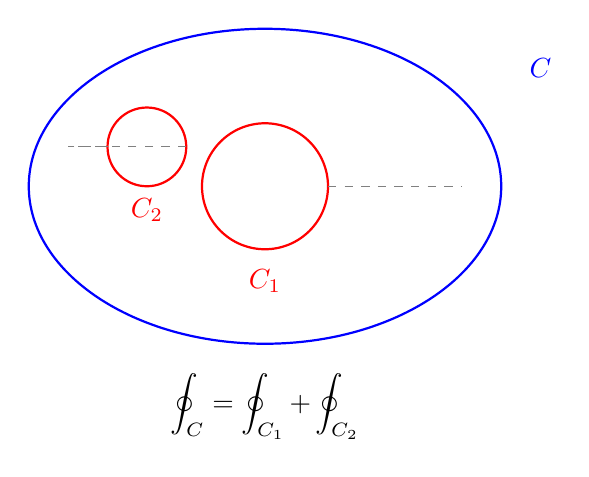
\begin{tikzpicture}[scale=1.0]
    % 外边界
    \draw[blue, thick, ->] (0,0) ellipse (3 and 2);
    \node[blue] at (3.5, 1.5) {$C$};
    
    % 内边界
    \draw[red, thick, <-] (0, 0) circle (0.8);
    \node[red] at (0, -1.2) {$C_1$};
    
    \draw[red, thick, <-] (-1.5, 0.5) circle (0.5);
    \node[red] at (-1.5, -0.3) {$C_2$};
    
    % 割线
    \draw[gray, dashed] (0.8, 0) -- (2.5, 0);
    \draw[gray, dashed] (-1, 0.5) -- (-2.5, 0.5);
    \draw[gray, dashed] (-2, 0.5) -- (-2.5, 0.5);
    
    \node at (0, -2.8) {$\displaystyle\oint_C = \oint_{C_1} + \oint_{C_2}$};
\end{tikzpicture}
\caption{多连通区域：外边界积分等于内边界积分之和}
\label{fig:multi-connected}
\end{figure}

\begin{lizi}{}{}
计算 $\displaystyle\oint_C \frac{1}{z - z_0}\,\mathrm{d}z$，其中 $C$ 是包围 $z_0$ 的简单闭曲线。

\begin{jie}
    以 $z_0$ 为圆心、$r$ 为半径作小圆 $C_r$，取逆时针方向。
    
    由多连通区域的柯西积分定理\index{柯西积分定理}：
    \begin{equation}
        \oint_C \frac{1}{z - z_0}\,\mathrm{d}z = \oint_{C_r} \frac{1}{z - z_0}\,\mathrm{d}z
    \end{equation}
    
    在 $C_r$ 上，$z - z_0 = r\mathrm{e}^{\mathrm{i}\theta}$，$\mathrm{d}z = r\mathrm{i}\mathrm{e}^{\mathrm{i}\theta}\,\mathrm{d}\theta$：
    \begin{equation}
        \oint_{C_r} \frac{1}{z - z_0}\,\mathrm{d}z = \int_0^{2\pi} \frac{r\mathrm{i}\mathrm{e}^{\mathrm{i}\theta}}{r\mathrm{e}^{\mathrm{i}\theta}}\,\mathrm{d}\theta = \int_0^{2\pi} \mathrm{i}\,\mathrm{d}\theta = 2\pi\mathrm{i}
    \end{equation}
\end{jie}
\end{lizi}

\begin{tishi}[重要结论]
这个例子的结果非常重要：$\displaystyle\oint_C \frac{1}{z - z_0}\,\mathrm{d}z = 2\pi\mathrm{i}$（$z_0$ 在 $C$ 内部）。这是导出柯西积分公式的基础。
\end{tishi}

% ========== 第三节 ==========
\section{柯西积分公式}

\subsection{公式的推导}

\begin{dingli}{柯西积分公式}{}
设 $f(z)$ 在简单闭曲线 $C$ 所围区域 $D$ 内解析，在 $\bar{D} = D \cup C$ 上连续，$z_0$ 是 $D$ 内任意一点，则
\[
    f(z_0) = \frac{1}{2\pi\mathrm{i}}\oint_C \frac{f(z)}{z - z_0}\,\mathrm{d}z
\]
\end{dingli}

\begin{proof}
考虑积分 $\displaystyle\oint_C \frac{f(z)}{z - z_0}\,\mathrm{d}z$。

以 $z_0$ 为圆心、$r$ 为半径作小圆 $C_r$。由多连通区域的柯西积分定理\index{柯西积分定理}：
\begin{equation}
    \oint_C \frac{f(z)}{z - z_0}\,\mathrm{d}z = \oint_{C_r} \frac{f(z)}{z - z_0}\,\mathrm{d}z
\end{equation}

注意到 $f(z) = f(z_0) + [f(z) - f(z_0)]$，所以
\begin{equation}
    \oint_{C_r} \frac{f(z)}{z - z_0}\,\mathrm{d}z = f(z_0)\oint_{C_r} \frac{1}{z - z_0}\,\mathrm{d}z + \oint_{C_r} \frac{f(z) - f(z_0)}{z - z_0}\,\mathrm{d}z
\end{equation}

第一项等于 $f(z_0) \cdot 2\pi\mathrm{i}$。

对于第二项，由于 $f(z)$ 连续，对于任意 $\varepsilon > 0$，存在 $\delta > 0$，当 $|z - z_0| < \delta$ 时，$|f(z) - f(z_0)| < \varepsilon$。

取 $r < \delta$，则
\begin{equation}
    \left|\oint_{C_r} \frac{f(z) - f(z_0)}{z - z_0}\,\mathrm{d}z\right| \leq \frac{\varepsilon}{r} \cdot 2\pi r = 2\pi\varepsilon
\end{equation}

由 $\varepsilon$ 的任意性，第二项为零。因此
\begin{equation}
    \oint_C \frac{f(z)}{z - z_0}\,\mathrm{d}z = 2\pi\mathrm{i} f(z_0)
\end{equation}
\end{proof}

\begin{wulibj}[物理意义：平均值性质]
柯西积分公式表明：解析函数\index{解析函数}在一点的值等于它在该点周围边界上的``平均值''（加权积分）。这说明解析函数\index{解析函数}的值由边界值完全确定，体现了解析函数\index{解析函数}的``刚性''。
\end{wulibj}

\begin{tishi}[深入理解：解析函数的``刚性'']
柯西积分公式揭示了解析函数\index{解析函数}的一个惊人性质——让我们来仔细品味一下。

公式告诉我们：只要知道了解析函数\index{解析函数} $f(z)$ 在边界 $C$ 上的值，就能唯一确定它在整个区域内部的值！

这和实变函数完全不同。对于实函数 $y = f(x)$，知道 $f(0) = 1$，你无法确定 $f(0.5)$ 是多少——可能有无数种函数通过 $(0, 1)$ 这个点。但解析函数\index{解析函数}不同：知道了边界上的值，内部就完全确定了。

这就是所谓的``刚性''：解析函数\index{解析函数}就像一块刚性的板，你不能随意弯曲它——一旦固定了边界，整块板就固定了。

更进一步，高阶导数公式告诉我们：解析函数\index{解析函数}在某点的各阶导数也都由边界值决定！这意味着：
\begin{enumerate}
    \item 解析函数\index{解析函数}在一点知道它的值，就知道了它所有导数的值，从而知道了它在整个邻域内的值（泰勒展开）。
    \item 解析函数\index{解析函数}不可能只在某个小区域为零——如果它在一段弧上为零，就必须在整个区域内为零。
    \item 解析函数\index{解析函数}不可能有``局部极值''——最大模原理说 $|f(z)|$ 的最大值只能在边界上达到。
\end{enumerate}

这些性质都源于一个核心：解析函数\index{解析函数}是一个高度``约束''的对象，它的各个部分紧密联系，牵一发而动全身。
\end{tishi}

\subsection{柯西积分公式的应用}

\begin{lizi}{}{}
计算 $\displaystyle\oint_C \frac{\mathrm{e}^z}{z - 1}\,\mathrm{d}z$，其中 $C$ 是 $|z| = 2$（逆时针方向）。

\begin{jie}
    $f(z) = \mathrm{e}^z$ 在 $C$ 内解析，$z_0 = 1$ 在 $C$ 内。
    
    由柯西积分公式：
    \begin{equation}
        \oint_C \frac{\mathrm{e}^z}{z - 1}\,\mathrm{d}z = 2\pi\mathrm{i} f(1) = 2\pi\mathrm{i} \cdot \mathrm{e}
    \end{equation}
\end{jie}
\end{lizi}

% ========== 第六节 ==========
\section{柯西积分公式的直接推论}

\subsection{高阶导数公式}

\begin{dingli}{高阶导数公式}{}
在柯西积分公式的条件下，$f(z)$ 在 $D$ 内有\keyword{任意阶导数}，且
\[
    f^{(n)}(z_0) = \frac{n!}{2\pi\mathrm{i}}\oint_C \frac{f(z)}{(z - z_0)^{n+1}}\,\mathrm{d}z
\]
\end{dingli}

\begin{proof}
对柯西积分公式两边对 $z_0$ 求导。形式地，
\begin{align}
    f'(z_0) &= \frac{1}{2\pi\mathrm{i}}\oint_C \frac{f(z)}{(z - z_0)^2}\,\mathrm{d}z \\
    f''(z_0) &= \frac{2}{2\pi\mathrm{i}}\oint_C \frac{f(z)}{(z - z_0)^3}\,\mathrm{d}z
\end{align}
一般地，归纳可得结论。严格证明需要验证积分号下求导的合法性。
\end{proof}

\begin{tishi}[惊人结论]
解析函数\index{解析函数}有任意阶导数！这是与实变函数的根本区别。一个实函数可以一阶可导但二阶不可导，但复变函数一旦可导就无穷次可导。
\end{tishi}

\begin{lizi}{}{}
计算 $\displaystyle\oint_C \frac{\sin z}{(z - \mathrm{i})^3}\,\mathrm{d}z$，其中 $C$ 是 $|z| = 2$。

\begin{jie}
    $f(z) = \sin z$，$z_0 = \mathrm{i}$，$n = 2$。
    
    由高阶导数公式：
    \begin{equation}
        \oint_C \frac{\sin z}{(z - \mathrm{i})^3}\,\mathrm{d}z = \frac{2\pi\mathrm{i}}{2!} f''(\mathrm{i})
    \end{equation}
    
    $f''(z) = -\sin z$，所以 $f''(\mathrm{i}) = -\sin(\mathrm{i}) = -\mathrm{i}\sinh(1)$。
    
    因此
    \begin{equation}
        \oint_C \frac{\sin z}{(z - \mathrm{i})^3}\,\mathrm{d}z = \pi\mathrm{i} \cdot (-\mathrm{i}\sinh(1)) = \pi\sinh(1)
    \end{equation}
\end{jie}
\end{lizi}

% ========== 第七节 ==========
\section{解析性的积分判据：莫雷拉定理（选读）}

\begin{wulibj}[为什么把莫雷拉定理放在章末]
到前一节为止，本章主线其实已经完整了：复积分的定义、柯西积分定理\index{柯西积分定理}、多连通区域中的典型闭路积分、柯西积分公式以及高阶导数公式，这些内容已经足以支撑下一章的泰勒展开。

莫雷拉\index{莫雷拉@莫雷拉（Morera）}（Morera）定理回答的是一个反方向的问题：如果我们只知道某个连续函数对任意闭曲线的积分都为零，能不能反过来推出它解析？这个问题很漂亮，也很重要，但它更像是对本章主线的一次回看，因此放在章末作为选读更合适。
\end{wulibj}

\subsection{莫雷拉定理}

\begin{dingli}{莫雷拉定理}{}
设 $f(z)$ 在区域 $D$ 内连续，且对于 $D$ 内任意简单闭曲线 $C$，有 $\oint_C f(z)\,\mathrm{d}z = 0$，则 $f(z)$ 在 $D$ 内解析。
\end{dingli}

\begin{proof}
由条件，积分 $\int_{z_0}^z f(\zeta)\,\mathrm{d}\zeta$ 与路径无关。定义
\begin{equation}
    F(z) = \int_{z_0}^z f(\zeta)\,\mathrm{d}\zeta
\end{equation}
类似于柯西积分定理\index{柯西积分定理}证明的逆过程，可以证明 $F'(z) = f(z)$。

因此 $f(z)$ 是 $F(z)$ 的导数。由于解析函数\index{解析函数}的导数仍解析（高阶导数公式的推论），$f(z)$ 在 $D$ 内解析。
\end{proof}

\begin{tishi}[柯西积分定理的逆定理]
    莫雷拉\index{莫雷拉@莫雷拉（Morera）}（Morera）定理是柯西积分定理\index{柯西积分定理}的逆定理。两者结合，我们得到：
\begin{equation}
    f \text{ 解析} \quad \Longleftrightarrow \quad \oint_C f(z)\,\mathrm{d}z = 0 \text{（对任意闭曲线）}
\end{equation}
\end{tishi}

\begin{tishi}[和下一章的衔接]
刘维尔定理和最大模原理虽然同样从柯西积分公式长出来，但它们更适合和泰勒展开、解析函数刚性放在一起系统讨论。因此它们将放到下一章``解析函数的整体性质与刚性''中出现。这样安排以后，本章主线会更集中，下一章的逻辑也会更顺。
\end{tishi}

% ========== 本章小结 ==========
\section{本章小结}

\subsection{核心定理}

\begin{enumerate}
    \item \textbf{有原函数时的复积分基本公式}：$\displaystyle \int_C f(z)\,\mathrm{d}z = F(z_2)-F(z_1)$
    \item \textbf{柯西积分定理\index{柯西积分定理}}：单连通区域内解析函数\index{解析函数}沿闭曲线积分等于零
    \item \textbf{单连通区域中的原函数存在性}：解析函数在单连通区域内存在原函数
    \item \textbf{柯西积分公式}：$\displaystyle f(z_0) = \frac{1}{2\pi\mathrm{i}}\oint_C \frac{f(z)}{z - z_0}\,\mathrm{d}z$
    \item \textbf{高阶导数公式}：$\displaystyle f^{(n)}(z_0) = \frac{n!}{2\pi\mathrm{i}}\oint_C \frac{f(z)}{(z - z_0)^{n+1}}\,\mathrm{d}z$
    \item \textbf{莫雷拉定理（选读）}：闭路积分为零可反推函数解析
\end{enumerate}

\subsection{重要结论}

\begin{itemize}
    \item 在单连通区域里，解析函数\index{解析函数}的积分与路径无关，并且存在原函数
    \item 典型闭路积分 $\displaystyle\oint_C \frac{1}{z-z_0}\,\mathrm{d}z = 2\pi\mathrm{i}$ 是柯西积分公式的基础
    \item 解析函数\index{解析函数}在一点的值和各阶导数都可以由边界积分表示
    \item 下一章的泰勒展开、刘维尔定理和最大模原理，都将从本章结果继续生长出来
\end{itemize}

% ========== 习题 ==========
\section{习题}

\textbf{基础题}

\begin{enumerate}
    \item 计算下列积分：
    \begin{enumerate}
        \item $\displaystyle\int_C z^2\,\mathrm{d}z$，$C$ 是从 $0$ 到 $1 + \mathrm{i}$ 的直线段
        \item 分别沿两条路径计算 $\displaystyle\int_C \overline{z}\,\mathrm{d}z$：一路径为从 $0$ 到 $1+\mathrm{i}$ 的直线段，另一路径先沿实轴从 $0$ 到 $1$，再沿竖直线段从 $1$ 到 $1+\mathrm{i}$
    \end{enumerate}
    
    \item 利用柯西积分公式计算：
    \begin{enumerate}
        \item $\displaystyle\oint_C \frac{\cos z}{z - \pi}\,\mathrm{d}z$，$C$ 是 $|z| = 4$
        \item $\displaystyle\oint_C \frac{\mathrm{e}^z}{z^2}\,\mathrm{d}z$，$C$ 是 $|z| = 1$
    \end{enumerate}
\end{enumerate}

\textbf{综合题}

\begin{enumerate}[resume]
    \item 设 $f(z)$ 在区域 $D$ 内有原函数 $F(z)$。证明：$f(z)$ 在 $D$ 内的积分与路径无关，并说明为什么任意闭曲线上的积分都为零。
    
    \item 计算 $\displaystyle\oint_C \frac{z}{(z - 1)(z - 2)}\,\mathrm{d}z$，其中 $C$ 分别为：
    \begin{enumerate}
        \item $|z| = 1.5$
        \item $|z| = 3$
    \end{enumerate}
    
    \item 说明为什么 $\displaystyle \frac{1}{z}$ 在穿孔平面 $\mathbb{C}\setminus\{0\}$ 上不可能有单值原函数。
\end{enumerate}

\textbf{挑战题}

\begin{enumerate}[resume]
    \item 用参数化方法直接证明：若 $C$ 是圆周 $|z-z_0|=r$ 的逆时针方向，则
    \[
        \oint_C \frac{1}{z-z_0}\,\mathrm{d}z = 2\pi\mathrm{i}.
    \]
    
    \item 设 $f(z)$ 在区域 $D$ 内连续，且对 $D$ 内任意闭曲线 $C$ 都有
    \[
        \oint_C f(z)\,\mathrm{d}z = 0.
    \]
    取定 $z_0\in D$，定义
    \[
        F(z)=\int_{z_0}^{z} f(\zeta)\,\mathrm{d}\zeta.
    \]
    试证明 $F'(z)=f(z)$，并说明这与莫雷拉定理有什么关系。
\end{enumerate}

% 第四章：复变函数的级数表示

\chapter{复变函数的级数表示}

\begin{wulibj}[本章导读]
\textbf{这一章我们要学什么？}

在高等数学中，大家已经学过泰勒展开——把一个光滑函数展开成无穷级数：
\[
    \mathrm{e}^x = 1 + x + \frac{x^2}{2!} + \frac{x^3}{3!} + \cdots
\]
这个展开式在 $x = 0$ 附近成立，而且越靠近 $0$，用前几项逼近就越精确。

现在问题来了：\textbf{复变函数能做同样的事情吗？}

答案是肯定的！而且复变函数的级数展开比实函数更加神奇：
\begin{itemize}
    \item \textbf{泰勒级数}：解析函数在解析点附近可以展开成幂级数，而且这个展开是\textbf{唯一}的——这导致了一个惊人的结论：``解析函数由它在一点附近的值完全决定''。实函数可没有这么强的性质！
    \item \textbf{洛朗级数}：当函数在某个点有奇点（比如 $\frac{1}{z}$ 在 $z = 0$），泰勒展开就不灵了。但洛朗展开可以处理这种情况——它允许出现负幂项。
    \item \textbf{奇点分类}：通过洛朗展开，我们可以精确地给奇点分类——可去奇点、极点、本性奇点，每种奇点都有独特的性质。
\end{itemize}

\textbf{学习建议}：本章内容与高等数学中的级数部分有很强的联系。如果你对实数项级数比较熟悉，学起来会轻松很多。如果有些遗忘，也没关系——我们会在第一节先回顾实数序列和级数的基本概念。
\end{wulibj}

% ========== 第一节 ==========
\section{级数预备知识}

\begin{tishi}[学习建议]
\textbf{为什么要先回顾实数序列和级数？}

复变函数的级数理论是建立在实数级数理论基础之上的。好消息是：大部分概念、定理和方法都可以直接推广到复数域！

具体来说：
\begin{itemize}
    \item 复数列的极限 $\Longleftrightarrow$ 实部、虚部分别收敛
    \item 复数项级数收敛 $\Longleftrightarrow$ 实部、虚部级数都收敛
    \item 比值判别法、根值判别法在复数域完全适用
\end{itemize}

如果你对实数序列和级数比较熟悉，可以跳过本节的第\ref{subsec:real-sequence}、\ref{subsec:real-series}小节，直接从第\ref{subsec:complex-sequence}小节开始阅读。如果有些概念记不太清了，建议耐心地把预备知识看一看——磨刀不误砍柴工！
\end{tishi}

% ---------- 实数序列 ----------
\subsection{实数序列}
\label{subsec:real-sequence}

\subsubsection{序列的概念}

在正式讨论序列之前，让我们先看一个简单的例子。

\begin{lizi}{}{}
    观察以下数列：
    \[
        1,\ \frac{1}{2},\ \frac{1}{3},\ \frac{1}{4},\ \frac{1}{5},\ \ldots
    \]
    这个数列的第 $n$ 项是什么？当 $n$ 越来越大时，第 $n$ 项的值会如何变化？
    
    \begin{jie}
        第 $n$ 项是 $\dfrac{1}{n}$。当 $n$ 越来越大时，$\dfrac{1}{n}$ 越来越接近 $0$。我们说这个数列``趋向于'' $0$。
    \end{jie}
\end{lizi}

\begin{dingliyi}{}{序列}
一个\textbf{序列}（或数列）是按一定顺序排列的一列数，记作
\begin{equation}
    a_1,\ a_2,\ a_3,\ \ldots,\ a_n,\ \ldots
\end{equation}
简记为 $\{a_n\}$，其中 $a_n$ 称为序列的\textbf{第 $n$ 项}或\textbf{通项}。
\end{dingliyi}

序列本质上是定义在正整数集上的函数：$a_n = f(n)$，$n = 1, 2, 3, \ldots$

\subsubsection{序列极限的直观理解}

在刚才的例子中，我们看到 $\frac{1}{n}$ 随着 $n$ 增大而越来越接近 $0$。这种``越来越接近''的感觉，正是极限概念的源头。

但是，``越来越接近''这个说法太模糊了。请看下面这个序列：

\begin{lizi}{}{}
    观察序列：$0,\ 1,\ 0,\ 1,\ 0,\ 1,\ \ldots$
    
    \begin{jie}
        这个序列在 $0$ 和 $1$ 之间来回振荡。它经常很接近 $0$，也经常很接近 $1$，但我们不能说它``趋向于''某个数。
        
        这说明：光说``越来越接近''是不够的，我们需要更精确的说法。
    \end{jie}
\end{lizi}

那么，什么才叫``真正地趋向于某个数''呢？

\textbf{关键想法}：不管你要求的误差有多小，只要 $n$ 足够大，$a_n$ 和 $a$ 的距离就能小于这个误差。

但在给出正式定义之前，让我们先看一个反例，理解为什么光说``越来越接近''是不够的。

\begin{lizi}{}{}
    观察序列：$0,\ 1,\ 0,\ 1,\ 0,\ 1,\ \ldots$
    
    \begin{jie}
        这个序列在 $0$ 和 $1$ 之间来回振荡。它经常很接近 $0$，也经常很接近 $1$，
        但我们不能说它``趋向于''某个数。
        
        这说明：光说``越来越接近''是不够的！必须要求``最终一直保持接近''，
        而不是``时近时远''。
    \end{jie}
\end{lizi}

\textbf{正确的感觉应该是}：不管你要求的误差有多小，只要 $n$ 足够大，$a_n$ 和 $a$ 的距离就能小于这个误差，而且从那以后\textbf{一直}保持在这个范围内。

这就是``要多接近有多接近''——把这句话翻译成数学语言，就得到下面的严格定义。

\begin{dingliyi}{}{序列极限（直观描述）}
如果当 $n$ 越来越大时，$a_n$ 越来越接近某个固定的数 $a$，而且可以``要多接近有多接近''，我们就说序列 $\{a_n\}$ 的\textbf{极限}是 $a$，记作
\begin{equation}
    \lim_{n \to \infty} a_n = a \quad \text{或} \quad a_n \to a \quad (n \to \infty)
\end{equation}
这时也称序列 $\{a_n\}$ \textbf{收敛}于 $a$。如果不存在这样的数 $a$，则称序列\textbf{发散}。
\end{dingliyi}

\subsubsection{序列极限的严格定义}

``越来越接近''只是一个直观说法，不够精确。我们需要用数学语言把这个意思说清楚。

\textbf{核心问题}：怎么用数学语言描述``要多接近有多接近''？

\textbf{思路}：
\begin{enumerate}
    \item ``接近程度''用距离 $|a_n - a|$ 来衡量
    \item ``要多接近''意味着：你给出一个允许的误差 $\varepsilon$（epsilon，读作``艾普西龙''）
    \item ``有多接近''意味着：我能找到一个位置 $N$，从那之后所有的项都满足要求
\end{enumerate}

\begin{dingliyi}{}{序列极限（epsilon-N 定义）}
设 $\{a_n\}$ 是一个序列，$a$ 是一个实数。如果对于任意 $\varepsilon > 0$，存在正整数 $N$，使得当 $n > N$ 时，有
\begin{equation}
    |a_n - a| < \varepsilon
\end{equation}
则称序列 $\{a_n\}$ 的极限是 $a$，记作 $\lim_{n \to \infty} a_n = a$。
\end{dingliyi}

\textbf{怎么理解这个定义？}

想象一场对话：
\begin{quote}
    \textbf{挑战者}：你能让序列的项和极限的距离小于 $0.1$ 吗？\\
    \textbf{回答者}：能！从第 $N_1$ 项开始，距离都小于 $0.1$。\\[3pt]
    \textbf{挑战者}：那小于 $0.01$ 呢？\\
    \textbf{回答者}：能！从第 $N_2$ 项开始，距离都小于 $0.01$。\\[3pt]
    \textbf{挑战者}：那小于 $0.001$ 呢？小于 $0.0001$ 呢？小于任意小的数 $\varepsilon$ 呢？\\
    \textbf{回答者}：都能！不管你给多小的 $\varepsilon$，我都能找到对应的 $N$！
\end{quote}

如果回答者能应对所有挑战，序列就收敛。这就叫``要多接近有多接近''。

\begin{figure}[htbp]
\centering
\begin{tikzpicture}[scale=0.9]
    % 坐标轴
    \draw[->, gray] (-0.5, 0) -- (8, 0) node[right] {$n$};
    \draw[->, gray] (0, -0.5) -- (0, 4) node[above] {$a_n$};
    
    % 极限值
    \draw[dashed, blue, thick] (-0.3, 1) -- (7.5, 1) node[right] {$a$（极限）};
    
    % epsilon 带
    \fill[blue!10, opacity=0.5] (-0.3, 0.5) rectangle (7.5, 1.5);
    \draw[dashed, blue] (-0.3, 1.5) -- (7.5, 1.5) node[right] {$a + \varepsilon$};
    \draw[dashed, blue] (-0.3, 0.5) -- (7.5, 0.5) node[right] {$a - \varepsilon$};
    
    % 序列点
    \foreach \n/\y in {1/3.2, 2/2.4, 3/1.9, 4/1.6, 5/1.4, 6/1.25, 7/1.15} {
        \fill[red] (\n, \y) circle (2pt);
    }
    
    % N 标记
    \draw[thick, green!60!black] (4, -0.3) -- (4, 3.5);
    \node[green!60!black, below] at (4, -0.3) {$N$};
    
    % 标注
    \node[above] at (2, 3.2) {\small 前 $N$ 项：可能不在带内};
    \node[above right] at (5.5, 1.5) {\small $n > N$：都在带内};
    
    % epsilon 标注
    \draw[<->, thick, blue] (7.8, 0.5) -- (7.8, 1.5);
    \node[blue, right] at (7.9, 1) {$2\varepsilon$};
\end{tikzpicture}
\caption{$\varepsilon$-$N$ 定义的直观理解：从某项开始，所有点都落入 $\varepsilon$ 带内}
\label{fig:epsilon-n}
\end{figure}

\begin{tishi}[如何理解 $\varepsilon$-$N$ 定义]
\begin{itemize}
    \item $\varepsilon$ 代表``误差容忍度''——你允许序列的项与极限值有多大的偏差。
    \item $N$ 代表``从哪里开始满足要求''——前 $N$ 项可以不满足要求，但从第 $N+1$ 项开始必须满足。
    \item ``对于任意 $\varepsilon > 0$''意思是无论你要求多精确，我都能满足。
    \item ``存在 $N$''意思是总有一个起点，从那里开始序列就``足够接近''极限了。
    \item \textbf{注意}：$N$ 依赖于 $\varepsilon$，$\varepsilon$ 越小，需要的 $N$ 通常越大。
\end{itemize}
\end{tishi}

\begin{lizi}{}{}
    用 $\varepsilon$-$N$ 定义证明：$\displaystyle\lim_{n \to \infty} \frac{1}{n} = 0$。
    
    \begin{jie}
        \textbf{怎么想}：我们要找到一个 $N$，使得当 $n > N$ 时，
        $\left|\frac{1}{n} - 0\right| < \varepsilon$。
        
        这等价于 $\frac{1}{n} < \varepsilon$，即 $n > \frac{1}{\varepsilon}$。
        
        所以，只要取 $N$ 为 $\frac{1}{\varepsilon}$ 的整数部分就行了！
        
        \textbf{正式证明}：
        对于任意 $\varepsilon > 0$，要使
        \[
            \left| \frac{1}{n} - 0 \right| < \varepsilon
        \]
        即 $\dfrac{1}{n} < \varepsilon$，只需 $n > \dfrac{1}{\varepsilon}$。
        
        因此，取 $N = \left\lfloor \dfrac{1}{\varepsilon} \right\rfloor$（即 $\dfrac{1}{\varepsilon}$ 的整数部分），则当 $n > N$ 时，必有
        \[
            \left| \frac{1}{n} - 0 \right| < \varepsilon
        \]
        由定义，$\displaystyle\lim_{n \to \infty} \frac{1}{n} = 0$。
    \end{jie}
\end{lizi}

\begin{lizi}{}{}
    用 $\varepsilon$-$N$ 定义证明：$\displaystyle\lim_{n \to \infty} \frac{n}{n+1} = 1$。
    
    \begin{jie}
        \textbf{怎么想}：先简化 $|a_n - 1|$，看看它实际上等于什么。
        \[
            \left| \frac{n}{n+1} - 1 \right| = \left| \frac{-1}{n+1} \right| = \frac{1}{n+1}
        \]
        要让它小于 $\varepsilon$，只需 $\frac{1}{n+1} < \varepsilon$，即 $n > \frac{1}{\varepsilon} - 1$。
        
        \textbf{正式证明}：
        对于任意 $\varepsilon > 0$，要使
        \[
            \left| \frac{n}{n+1} - 1 \right| = \left| \frac{-1}{n+1} \right| = \frac{1}{n+1} < \varepsilon
        \]
        只需 $n + 1 > \dfrac{1}{\varepsilon}$，即 $n > \dfrac{1}{\varepsilon} - 1$。
        
        取 $N = \max\left\{1, \left\lfloor \dfrac{1}{\varepsilon} \right\rfloor\right\}$，则当 $n > N$ 时，必有
        \[
            \left| \frac{n}{n+1} - 1 \right| < \varepsilon
        \]
        由定义，$\displaystyle\lim_{n \to \infty} \frac{n}{n+1} = 1$。
    \end{jie}
\end{lizi}

\subsubsection{序列极限的性质}

极限有哪些基本性质呢？我们来看看。

\begin{dingli}{}{极限的唯一性}
如果序列 $\{a_n\}$ 收敛，则它的极限唯一。
\end{dingli}

\begin{tishi}[证明思路]
要证明极限唯一，我们用反证法：假设有两个不同的极限 $a$ 和 $b$。

关键观察：当 $n$ 充分大时，$a_n$ 同时接近 $a$ 和 $b$。如果 $a \neq b$，这怎么可能呢？

具体做法：
\begin{enumerate}
    \item 设 $a \neq b$，那么 $|a - b| > 0$
    \item 当 $n$ 很大时，$|a_n - a|$ 和 $|a_n - b|$ 都可以很小
    \item 但 $|a - b| \leq |a_n - a| + |a_n - b|$（三角不等式）
    \item 右边可以任意小，左边是正数，矛盾！
\end{enumerate}
\end{tishi}

\begin{proof}
设 $\lim_{n \to \infty} a_n = a$ 且 $\lim_{n \to \infty} a_n = b$。我们要证明 $a = b$。

对于任意 $\varepsilon > 0$，存在 $N_1$ 使得当 $n > N_1$ 时，$|a_n - a| < \varepsilon/2$；存在 $N_2$ 使得当 $n > N_2$ 时，$|a_n - b| < \varepsilon/2$。

取 $N = \max\{N_1, N_2\}$，则当 $n > N$ 时，
\[
    |a - b| = |a - a_n + a_n - b| \leq |a_n - a| + |a_n - b| < \frac{\varepsilon}{2} + \frac{\varepsilon}{2} = \varepsilon
\]
由于 $\varepsilon$ 是任意正数，要使上式成立，必有 $|a - b| = 0$，即 $a = b$。
\end{proof}

\begin{dingli}{}{极限的运算法则}
设 $\lim_{n \to \infty} a_n = a$，$\lim_{n \to \infty} b_n = b$，则
\begin{enumerate}
    \item $\displaystyle\lim_{n \to \infty} (a_n + b_n) = a + b$
    \item $\displaystyle\lim_{n \to \infty} (a_n - b_n) = a - b$
    \item $\displaystyle\lim_{n \to \infty} (a_n \cdot b_n) = a \cdot b$
    \item 若 $b \neq 0$，则 $\displaystyle\lim_{n \to \infty} \frac{a_n}{b_n} = \frac{a}{b}$
\end{enumerate}
\end{dingli}

\begin{tishi}[证明思路——为什么这些运算法则成立？]
直观上，如果 $a_n \approx a$，$b_n \approx b$，那么：
\begin{itemize}
    \item $a_n + b_n \approx a + b$（和的极限等于极限的和）
    \item $a_n \cdot b_n \approx a \cdot b$（积的极限等于极限的积）
\end{itemize}

但严格证明需要用 $\varepsilon$-$N$ 语言。关键技巧：
\begin{enumerate}
    \item \textbf{和的极限}：用三角不等式 $|(a_n+b_n)-(a+b)| \leq |a_n-a| + |b_n-b|$
    \item \textbf{积的极限}：关键变形 $|a_n b_n - ab| = |a_n b_n - a_n b + a_n b - ab|$，这叫``加一项减一项''技巧
    \item \textbf{商的极限}：转化为积的极限，$\frac{a_n}{b_n} = a_n \cdot \frac{1}{b_n}$
\end{enumerate}
\end{tishi}

\begin{proof}
我们依次证明各条结论。

\textbf{(1) 和的极限}：核心是三角不等式 $|(a_n+b_n)-(a+b)| \leq |a_n-a| + |b_n-b|$。

由于 $a_n \to a$，当 $n$ 充分大时 $|a_n-a|$ 可任意小；同理 $|b_n-b|$ 也可任意小。
因此它们的和也可任意小，即 $a_n + b_n \to a + b$。

\textbf{(2) 差的极限}：与(1)类似，$|(a_n-b_n)-(a-b)| \leq |a_n-a| + |b_n-b|$。

\textbf{(3) 积的极限}：关键变形是``加一项减一项''：
\[
    |a_n b_n - ab| = |a_n b_n - a_n b + a_n b - ab| 
    \leq |a_n||b_n - b| + |b||a_n - a|
\]
由于 $\{a_n\}$ 收敛，它有界，设 $|a_n| \leq M$。
再由 $a_n \to a$ 和 $b_n \to b$，右端两项都可任意小。

\textbf{(4) 商的极限}：转化为积的极限，$\frac{a_n}{b_n} = a_n \cdot \frac{1}{b_n}$。
关键是证明 $\frac{1}{b_n} \to \frac{1}{b}$（当 $b \neq 0$ 时）：
\[
    \left|\frac{1}{b_n} - \frac{1}{b}\right| = \frac{|b_n - b|}{|b_n||b|}
\]
由于 $b_n \to b \neq 0$，当 $n$ 充分大时 $|b_n| > |b|/2$，分母有下界；
分子 $|b_n - b|$ 可任意小，故整体可任意小。

证毕。
\end{proof}

这些运算法则告诉我们：极限运算可以和四则运算交换顺序。

\begin{lizi}{}{}
    求 $\displaystyle\lim_{n \to \infty} \frac{2n + 1}{3n - 2}$。
    
    \begin{jie}
        将分子分母同时除以 $n$：
        \[
            \lim_{n \to \infty} \frac{2n + 1}{3n - 2} = \lim_{n \to \infty} \frac{2 + \frac{1}{n}}{3 - \frac{2}{n}} = \frac{2 + 0}{3 - 0} = \frac{2}{3}
        \]
        这里用到了 $\displaystyle\lim_{n \to \infty} \frac{1}{n} = 0$ 和极限的除法法则。
    \end{jie}
\end{lizi}

\begin{lizi}{}{}
    求 $\displaystyle\lim_{n \to \infty} \frac{n^2 + 2n}{n^2 - 1}$。
    
    \begin{jie}
        将分子分母同时除以 $n^2$：
        \[
            \lim_{n \to \infty} \frac{n^2 + 2n}{n^2 - 1} = \lim_{n \to \infty} \frac{1 + \frac{2}{n}}{1 - \frac{1}{n^2}} = \frac{1 + 0}{1 - 0} = 1
        \]
    \end{jie}
\end{lizi}

\begin{tishi}[分式序列极限的技巧]
对于形如 $\dfrac{a_n}{b_n}$ 的分式序列，其中 $a_n$ 和 $b_n$ 都是多项式或多项式之比，常用的技巧是将分子分母同除以最高次项，然后利用 $\lim_{n \to \infty} \frac{1}{n^k} = 0$（$k > 0$）求极限。
\end{tishi}

% ---------- 实数项级数 ----------
\subsection{实数项级数}
\label{subsec:real-series}

\subsubsection{级数的概念}

序列讨论的是一列数的``终点''，而级数讨论的是一列数的``累加''。

\textbf{一个启发性的问题}：

芝诺悖论中说：阿基里斯要追上乌龟，必须先走到乌龟的起点，但这时乌龟又往前爬了一点；然后再追到乌龟的新位置，乌龟又往前爬了一点…… 这样看来，阿基里斯永远追不上乌龟？

用数学语言来说：$1 + \frac{1}{2} + \frac{1}{4} + \frac{1}{8} + \cdots$ 等于多少？

直觉告诉我们，这个和应该是 $2$（阿基里斯确实能追上乌龟）。但无穷多个数相加，怎么定义它的``和''呢？

\textbf{关键想法}：用部分和的极限来定义！

\begin{dingliyi}{}{级数与部分和}
设 $\{a_n\}$ 是一个序列，表达式
\begin{equation}
    a_1 + a_2 + a_3 + \cdots = \sum_{n=1}^{\infty} a_n
\end{equation}
称为\textbf{级数}，其中 $a_n$ 称为级数的\textbf{第 $n$ 项}或\textbf{通项}。

级数的\textbf{部分和}定义为
\begin{equation}
    S_n = \sum_{k=1}^{n} a_k = a_1 + a_2 + \cdots + a_n
\end{equation}
\end{dingliyi}

\begin{dingliyi}{}{级数收敛与发散}
如果部分和序列 $\{S_n\}$ 收敛，即 $\lim_{n \to \infty} S_n = S$ 存在，则称级数 $\sum_{n=1}^{\infty} a_n$ \textbf{收敛}，$S$ 称为级数的\textbf{和}，记作
\begin{equation}
    \sum_{n=1}^{\infty} a_n = S
\end{equation}
如果 $\{S_n\}$ 发散，则称级数\textbf{发散}。
\end{dingliyi}

\begin{tishi}[级数与序列的关系]
\begin{itemize}
    \item 序列 $\{a_n\}$ 是一列数，我们关心它的``极限''。
    \item 级数 $\sum a_n$ 是一列数的``累加''，我们关心部分和序列 $\{S_n\}$ 的极限。
    \item 级数收敛 $\Longleftrightarrow$ 部分和序列收敛。
\end{itemize}
\end{tishi}

\subsubsection{最重要的级数：几何级数}

在所有级数中，几何级数是最重要、最基本的。它将反复出现在本章的各个角落，甚至可以说：\textbf{理解了几何级数，就理解了级数理论的一半}。

\begin{dingliyi}{}{几何级数}
形如
\begin{equation}
    \sum_{n=0}^{\infty} r^n = 1 + r + r^2 + r^3 + \cdots
\end{equation}
的级数称为\textbf{几何级数}（或等比级数），其中 $r$ 称为\textbf{公比}。
\end{dingliyi}

\textbf{几何级数的部分和怎么求？}

部分和是 $S_n = 1 + r + r^2 + \cdots + r^n$。直接相加？每一项都在变，太麻烦了。

\textbf{观察}：这个求和有个特点——相邻两项的比值相同（都是 $r$）。

\textbf{技巧}：既然每项都是前一项乘以 $r$，那我把整个式子乘以 $r$，大部分项就会``对齐''！
\begin{align}
    S_n &= 1 + r + r^2 + \cdots + r^n \\
    rS_n &= \phantom{1 + {}} r + r^2 + r^3 + \cdots + r^{n+1}
\end{align}

看到了吗？下式比上式少了一个``1''，多了一个``$r^{n+1}$''。

相减，中间那些项全消掉了：
\[
    S_n - rS_n = 1 - r^{n+1}
\]

所以
\[
    S_n = \frac{1 - r^{n+1}}{1 - r} \quad \text{（当 $r \neq 1$）}
\]

\textbf{现在关键问题来了}：当 $n \to \infty$ 时，$S_n$ 趋向什么？

这取决于 $r^{n+1}$ 的行为：
\begin{itemize}
    \item 如果 $|r| < 1$，则 $r^{n+1} \to 0$，所以 $S_n \to \frac{1}{1-r}$
    \item 如果 $|r| \geq 1$，则 $r^{n+1}$ 不趋于 $0$，级数发散
\end{itemize}

\begin{dingli}{}{几何级数的收敛性}
几何级数 $\sum_{n=0}^{\infty} r^n$ 当 $|r| < 1$ 时收敛，当 $|r| \geq 1$ 时发散。当收敛时，其和为
\begin{equation}
    \boxed{\sum_{n=0}^{\infty} r^n = \frac{1}{1-r}, \quad |r| < 1}
\end{equation}
\end{dingli}

\begin{proof}
当 $|r| < 1$ 时，$\lim_{n \to \infty} r^{n+1} = 0$，所以
\[
    \lim_{n \to \infty} S_n = \lim_{n \to \infty} \frac{1 - r^{n+1}}{1 - r} = \frac{1 - 0}{1 - r} = \frac{1}{1 - r}
\]
当 $|r| \geq 1$ 时，通项 $r^n$ 不趋于 $0$，级数发散（见下文收敛必要条件）。
\end{proof}

\begin{jinshi}[几何级数的条件 $|r| < 1$]
几何级数收敛的充要条件是 $|r| < 1$。这个条件非常重要，请务必记住！
\begin{itemize}
    \item $r = 0.5$：$1 + 0.5 + 0.25 + 0.125 + \cdots = 2$（收敛）
    \item $r = 1$：$1 + 1 + 1 + \cdots$（发散，部分和趋向无穷）
    \item $r = 2$：$1 + 2 + 4 + 8 + \cdots$（发散，部分和趋向无穷）
    \item $r = -1$：$1 - 1 + 1 - 1 + \cdots$（发散，部分和在 $0$ 和 $1$ 之间振荡）
\end{itemize}
\end{jinshi}

\begin{figure}[htbp]
\centering
\begin{tikzpicture}[scale=0.85]
    % 坐标轴
    \draw[->, gray] (-0.5, 0) -- (7, 0) node[right] {$n$};
    \draw[->, gray] (0, -0.3) -- (0, 4.5) node[above] {$S_n$};
    
    % 极限值
    \draw[dashed, blue, thick] (-0.3, 2) -- (6.5, 2) node[right] {$\frac{1}{1-r} = 2$};
    
    % 部分和点 (r=0.5)
    \foreach \n/\s in {0/1, 1/1.5, 2/1.75, 3/1.875, 4/1.9375, 5/1.96875} {
        \fill[red] (\n, \s) circle (2.5pt);
    }
    
    % 连线
    \draw[red, thick] (0, 1) -- (1, 1.5) -- (2, 1.75) -- (3, 1.875) -- (4, 1.9375) -- (5, 1.96875);
    
    % 标注
    \node[red, above left] at (0, 1) {$S_0 = 1$};
    \node[red, above] at (2, 1.75) {$S_2 = 1.75$};
    \node[red, right] at (5, 1.96875) {$S_5 \approx 1.97$};
    
    % 标题
    \node at (3, 5.2) {$r = 0.5$ 时，部分和 $S_n$ 趋于极限 $2$};
    
    % 网格参考线
    \draw[gray, very thin, dashed] (-0.3, 1) -- (6.5, 1);
    \draw[gray, very thin, dashed] (-0.3, 1.5) -- (6.5, 1.5);
\end{tikzpicture}
\caption{几何级数 $\sum_{n=0}^{\infty} (0.5)^n$ 的部分和逐渐趋于极限 $2$}
\label{fig:geometric-series}
\end{figure}

\begin{lizi}{}{}
    求级数 $\displaystyle\sum_{n=1}^{\infty} \frac{1}{2^n}$ 的和。
    
    \begin{jie}
        $\displaystyle\sum_{n=1}^{\infty} \frac{1}{2^n} = \frac{1}{2} + \frac{1}{4} + \frac{1}{8} + \cdots$
        
        这是首项为 $\dfrac{1}{2}$、公比为 $r = \dfrac{1}{2}$ 的几何级数（从 $n=1$ 开始）。利用几何级数公式：
        \[
            \sum_{n=1}^{\infty} \frac{1}{2^n} = \frac{1}{2} \sum_{n=0}^{\infty} \left(\frac{1}{2}\right)^n = \frac{1}{2} \cdot \frac{1}{1 - \frac{1}{2}} = \frac{1}{2} \cdot 2 = 1
        \]
        
        或者直接套用从 $n=1$ 开始的几何级数公式：
        \[
            \sum_{n=1}^{\infty} r^n = \frac{r}{1-r}, \quad |r| < 1
        \]
        代入 $r = \dfrac{1}{2}$ 得 $\dfrac{\frac{1}{2}}{1 - \frac{1}{2}} = 1$。
    \end{jie}
\end{lizi}

\begin{lizi}{}{}
    将循环小数 $0.\overline{3} = 0.333\ldots$ 表示为分数。
    
    \begin{jie}
        $0.333\ldots = \dfrac{3}{10} + \dfrac{3}{100} + \dfrac{3}{1000} + \cdots$
        
        这是一个首项为 $\dfrac{3}{10}$、公比为 $r = \dfrac{1}{10}$ 的几何级数：
        \[
            0.333\ldots = \frac{3}{10} \sum_{n=0}^{\infty} \left(\frac{1}{10}\right)^n = \frac{3}{10} \cdot \frac{1}{1 - \frac{1}{10}} = \frac{3}{10} \cdot \frac{10}{9} = \frac{1}{3}
        \]
    \end{jie}
\end{lizi}

\subsubsection{级数收敛的必要条件}

一个级数要收敛，它的通项必须满足什么条件？

\begin{dingli}{}{级数收敛的必要条件}
若级数 $\displaystyle\sum_{n=1}^{\infty} a_n$ 收敛，则 $\displaystyle\lim_{n \to \infty} a_n = 0$。
\end{dingli}

\begin{proof}
设 $S_n = \sum_{k=1}^{n} a_k$ 是部分和，$S = \lim_{n \to \infty} S_n$。注意到
\[
    a_n = S_n - S_{n-1}
\]
取极限得
\[
    \lim_{n \to \infty} a_n = \lim_{n \to \infty} (S_n - S_{n-1}) = S - S = 0
\]
\end{proof}

\begin{jinshi}[必要条件 $\neq$ 充分条件]
$\lim_{n \to \infty} a_n = 0$ 只是级数收敛的\textbf{必要条件}，不是充分条件！

最著名的反例是\textbf{调和级数}：
\[
    \sum_{n=1}^{\infty} \frac{1}{n} = 1 + \frac{1}{2} + \frac{1}{3} + \frac{1}{4} + \cdots
\]
虽然通项 $\dfrac{1}{n} \to 0$，但这个级数发散！
\end{jinshi}

\subsubsection{绝对收敛与条件收敛}

\begin{dingliyi}{}{复数项级数的绝对收敛与条件收敛}
\begin{itemize}
    \item 若 $\displaystyle\sum_{n=1}^{\infty} |a_n|$ 收敛，则称 $\displaystyle\sum_{n=1}^{\infty} a_n$ \textbf{绝对收敛}。
    \item 若 $\displaystyle\sum_{n=1}^{\infty} a_n$ 收敛但 $\displaystyle\sum_{n=1}^{\infty} |a_n|$ 发散，则称 $\displaystyle\sum_{n=1}^{\infty} a_n$ \textbf{条件收敛}。
\end{itemize}
\end{dingliyi}

\begin{tishi}[为什么要区分绝对收敛和条件收敛？]
    表面上看，这只是``收敛速度快慢''的区别。但实际上有本质不同：
    
    \textbf{绝对收敛}：级数是``稳定''的，可以放心重排、相乘、交换积分和求和。
    
    \textbf{条件收敛}：级数是``脆弱''的，改变求和顺序可能改变和的值！
    
    \textbf{例子}：$1 - \frac{1}{2} + \frac{1}{3} - \frac{1}{4} + \cdots = \ln 2$，
    但重新排列项的顺序，可以使和变成任意数（黎曼重排定理）。
    
    这是因为条件收敛依赖于``正负项相互抵消''，一旦顺序改变，抵消方式就变了。
    
    \textbf{物理意义}：在物理中，级数常表示能量的叠加。绝对收敛意味着``总能量 = 各部分能量之和''，与叠加顺序无关，这符合物理直觉。条件收敛则可能导致``改变叠加顺序，总能量改变''，这在物理上是荒谬的。
    
    \textbf{一句话}：绝对收敛 $\Rightarrow$ 和客观存在；条件收敛 $\Rightarrow$ 和依赖于计算方式。
\end{tishi}

\begin{dingli}{}{绝对收敛蕴含收敛}
若级数 $\sum a_n$ 绝对收敛，则它收敛。
\end{dingli}

\begin{proof}
设 $\sum |a_n|$ 收敛。我们要证明 $\sum a_n$ 收敛。

\textbf{方法一：利用柯西准则}。

由 $\sum |a_n|$ 收敛，根据柯西收敛准则，对于任意 $\varepsilon > 0$，存在 $N$ 使得当 $n > m > N$ 时，
\[
    \sum_{k=m+1}^{n} |a_k| < \varepsilon
\]

对于 $\sum a_n$，由三角不等式，
\[
    \left|\sum_{k=m+1}^{n} a_k\right| \leq \sum_{k=m+1}^{n} |a_k| < \varepsilon
\]

由柯西收敛准则，$\sum a_n$ 收敛。

\textbf{方法二：利用正负部分解}。

定义
\[
    a_n^+ = \begin{cases} a_n, & a_n \geq 0 \\ 0, & a_n < 0 \end{cases}, \quad
    a_n^- = \begin{cases} 0, & a_n \geq 0 \\ -a_n, & a_n < 0 \end{cases}
\]

则 $a_n = a_n^+ - a_n^-$，且 $|a_n| = a_n^+ + a_n^-$。

由于 $0 \leq a_n^+ \leq |a_n|$ 且 $0 \leq a_n^- \leq |a_n|$，由比较判别法，$\sum a_n^+$ 和 $\sum a_n^-$ 都收敛。

因此
\[
    \sum a_n = \sum (a_n^+ - a_n^-) = \sum a_n^+ - \sum a_n^-
\]
收敛。

\textbf{注}：方法二不仅证明了收敛，还给出了求和公式：$\sum a_n = \sum a_n^+ - \sum a_n^-$。
\end{proof}

\begin{lizi}{}{}
    判断级数 $\displaystyle\sum_{n=1}^{\infty} \frac{(-1)^{n+1}}{n} = 1 - \frac{1}{2} + \frac{1}{3} - \frac{1}{4} + \cdots$ 的收敛类型。
    
    \begin{jie}
        这个级数是收敛的（可用莱布尼茨判别法证明）。
        
        但 $\displaystyle\sum_{n=1}^{\infty} \left|\frac{(-1)^{n+1}}{n}\right| = \sum_{n=1}^{\infty} \frac{1}{n}$ 是调和级数，发散。
        
        所以这是\textbf{条件收敛}的级数。其和为 $\ln 2$。
    \end{jie}
\end{lizi}

\begin{lizi}{}{}
    判断级数 $\displaystyle\sum_{n=1}^{\infty} \frac{(-1)^{n+1}}{n^2} = 1 - \frac{1}{4} + \frac{1}{9} - \frac{1}{16} + \cdots$ 的收敛类型。
    
    \begin{jie}
        $\displaystyle\sum_{n=1}^{\infty} \left|\frac{(-1)^{n+1}}{n^2}\right| = \sum_{n=1}^{\infty} \frac{1}{n^2}$，这是著名的 Basel 级数，收敛于 $\dfrac{\pi^2}{6}$。
        
        所以这个级数\textbf{绝对收敛}。
    \end{jie}
\end{lizi}

\subsubsection{收敛判别法}

如何判断一个级数是否收敛？以下是几个常用的判别法。

\begin{dingli}{}{比值判别法（达朗贝尔判别法）}
设 $\displaystyle\lim_{n \to \infty} \left|\frac{a_{n+1}}{a_n}\right| = \rho$，则
\begin{itemize}
    \item 若 $\rho < 1$，级数 $\sum a_n$ 绝对收敛；
    \item 若 $\rho > 1$，级数 $\sum a_n$ 发散；
    \item 若 $\rho = 1$，判别法失效，需要其他方法。
\end{itemize}
\end{dingli}

\begin{tishi}[比值判别法的直觉——为什么它能判断收敛性？]
关键想法：\textbf{和几何级数比较}。

如果 $\lim |a_{n+1}/a_n| = \rho < 1$，这意味着当 $n$ 充分大时：
\[
    |a_{n+1}| \approx \rho |a_n|
\]

这很像几何级数 $|a_n| \approx |a_N| \cdot \rho^{n-N}$ 的行为。既然 $\sum \rho^n$ 收敛，那 $\sum |a_n|$ 也应该收敛！

反过来，如果 $\rho > 1$，则 $|a_n|$ 越来越大，不可能趋于 $0$，所以级数发散。
\end{tishi}

\begin{proof}
\textbf{核心想法}：与几何级数比较。

\textbf{情况一：$\rho < 1$。}

取 $r$ 使得 $\rho < r < 1$（例如 $r = (1+\rho)/2$）。

由极限定义，当 $n$ 充分大时，$|a_{n+1}/a_n| < r$，即 $|a_{n+1}| < r|a_n|$。

这很像 $|a_n| \approx |a_N| \cdot r^{n-N}$ 的行为。由于 $\sum r^n$ 收敛（$r < 1$），
由比较判别法，$\sum |a_n|$ 也收敛。

\textbf{情况二：$\rho > 1$。}

当 $n$ 充分大时，$|a_{n+1}| > |a_n|$，即 $|a_n|$ 单调递增，不可能趋于 $0$，故级数发散。

\textbf{情况三：$\rho = 1$。}

以 $p$-级数 $\sum \frac{1}{n^p}$ 为例：$\lim \frac{n^p}{(n+1)^p} = 1$，但收敛性取决于 $p$。
故判别法失效。
\end{proof}

\begin{dingli}{}{根值判别法（柯西判别法）}
设 $\displaystyle\lim_{n \to \infty} \sqrt[n]{|a_n|} = \rho$，则
\begin{itemize}
    \item 若 $\rho < 1$，级数 $\sum a_n$ 绝对收敛；
    \item 若 $\rho > 1$，级数 $\sum a_n$ 发散；
    \item 若 $\rho = 1$，判别法失效，需要其他方法。
\end{itemize}
\end{dingli}

\begin{proof}
\textbf{情况一：$\rho < 1$。}

取 $\varepsilon > 0$ 使得 $\rho + \varepsilon < 1$。

由极限定义，存在 $N$ 使得当 $n \geq N$ 时，
\[
    \sqrt[n]{|a_n|} < \rho + \varepsilon =: r < 1
\]

即 $|a_n| < r^n$ 对 $n \geq N$ 成立。

几何级数 $\sum_{n=N}^{\infty} r^n$ 收敛（因为 $r < 1$），由比较判别法，$\sum_{n=N}^{\infty}|a_n|$ 收敛，故 $\sum a_n$ 绝对收敛。

\textbf{情况二：$\rho > 1$。}

取 $\varepsilon > 0$ 使得 $\rho - \varepsilon > 1$。

由极限定义，存在 $N$ 使得当 $n \geq N$ 时，
\[
    \sqrt[n]{|a_n|} > \rho - \varepsilon > 1
\]

即 $|a_n| > 1$ 对 $n \geq N$ 成立。

所以 $\lim_{n \to \infty} a_n \neq 0$，级数 $\sum a_n$ 发散。

\textbf{情况三：$\rho = 1$。}

同样以 $p$-级数为例。由 Stirling 公式或直接计算，
\[
    \lim_{n \to \infty}\sqrt[n]{\frac{1}{n^p}} = \lim_{n \to \infty}\frac{1}{n^{p/n}} = 1
\]

但 $p$-级数在 $p > 1$ 和 $p \leq 1$ 时收敛性不同，故 $\rho = 1$ 时判别法失效。
\end{proof}

\begin{dingli}{}{比较判别法}
若 $|a_n| \leq b_n$ 且 $\sum b_n$ 收敛，则 $\sum a_n$ 绝对收敛。

若 $|a_n| \geq b_n \geq 0$ 且 $\sum b_n$ 发散，则 $\sum a_n$ 发散。
\end{dingli}

\begin{proof}
\textbf{第一部分：收敛性。}

设 $|a_n| \leq b_n$ 且 $\sum b_n$ 收敛。

由柯西收敛准则，对于任意 $\varepsilon > 0$，存在 $N$ 使得当 $n > m > N$ 时，
\[
    \sum_{k=m+1}^{n} b_k < \varepsilon
\]

由于 $|a_k| \leq b_k$，有
\[
    \sum_{k=m+1}^{n} |a_k| \leq \sum_{k=m+1}^{n} b_k < \varepsilon
\]

由柯西收敛准则，$\sum |a_n|$ 收敛，即 $\sum a_n$ 绝对收敛。

\textbf{第二部分：发散性。}

设 $|a_n| \geq b_n \geq 0$ 且 $\sum b_n$ 发散。

假设 $\sum |a_n|$ 收敛。由于 $0 \leq b_n \leq |a_n|$，由第一部分的结论（逆否命题），$\sum b_n$ 应该收敛，矛盾。

因此 $\sum |a_n|$ 发散，从而 $\sum a_n$ 发散。

\textbf{注}：比较判别法是判断级数收敛性最基本的方法，比值判别法和根值判别法本质上都是与几何级数比较。
\end{proof}

\begin{lizi}{}{}
    判断级数 $\displaystyle\sum_{n=1}^{\infty} \frac{n}{2^n}$ 的收敛性。
    
    \begin{jie}
        用比值判别法：
        \[
            \lim_{n \to \infty} \left|\frac{a_{n+1}}{a_n}\right| = \lim_{n \to \infty} \frac{(n+1)/2^{n+1}}{n/2^n} = \lim_{n \to \infty} \frac{n+1}{2n} = \frac{1}{2} < 1
        \]
        所以级数绝对收敛。
    \end{jie}
\end{lizi}

\begin{lizi}{}{}
    判断级数 $\displaystyle\sum_{n=1}^{\infty} \frac{n!}{n^n}$ 的收敛性。
    
    \begin{jie}
        用比值判别法：
        \begin{align*}
            \lim_{n \to \infty} \frac{a_{n+1}}{a_n}
            &= \lim_{n \to \infty} \frac{(n+1)!/(n+1)^{n+1}}{n!/n^n} \\
            &= \lim_{n \to \infty} \frac{(n+1) \cdot n^n}{(n+1)^{n+1}} \\
            &= \lim_{n \to \infty} \left(\frac{n}{n+1}\right)^n
        \end{align*}
        
        注意到 $\left(\dfrac{n}{n+1}\right)^n = \left(1 - \dfrac{1}{n+1}\right)^n$，令 $m = n+1$：
        \begin{align*}
            \lim_{n \to \infty} \left(\frac{n}{n+1}\right)^n
            &= \lim_{m \to \infty} \left(1 - \frac{1}{m}\right)^{m-1} \\
            &= \lim_{m \to \infty} \frac{\left(1 - \frac{1}{m}\right)^m}{1 - \frac{1}{m}} \\
            &= \frac{e^{-1}}{1} = \frac{1}{e} < 1
        \end{align*}

        \textbf{为什么 $\left(1 - \frac{1}{m}\right)^m \to e^{-1}$？}

        这是重要极限 $\lim_{m \to \infty}\left(1 + \frac{1}{m}\right)^m = e$ 的变形。令 $t = -m$：
        \[
            \left(1 - \frac{1}{m}\right)^m = \left(1 + \frac{1}{t}\right)^{-t} = \left[\left(1 + \frac{1}{t}\right)^t\right]^{-1} \xrightarrow{t \to -\infty} e^{-1} = \frac{1}{e}
        \]
        或者直接用 $\lim_{x \to \infty}\left(1 + \frac{a}{x}\right)^x = e^a$ 这个更一般的结论（取 $a = -1$）。

        所以级数收敛。
    \end{jie}
\end{lizi}

\begin{tishi}[实数项级数预备知识小结]
\begin{enumerate}
    \item \textbf{序列}是按顺序排列的一列数；\textbf{级数}是序列的累加。
    \item 序列收敛 $\Longleftrightarrow$ 极限存在；级数收敛 $\Longleftrightarrow$ 部分和序列收敛。
    \item \textbf{几何级数}是最重要的基础级数：$\displaystyle\sum_{n=0}^{\infty} r^n = \frac{1}{1-r}$（$|r| < 1$）。
    \item 级数收敛的必要条件：通项趋于 $0$（但不是充分条件！）。
    \item \textbf{绝对收敛}的级数一定收敛；比值判别法和根值判别法是常用的判别工具。
\end{enumerate}
掌握了这些实数项级数的预备知识，我们就可以开始学习复数项级数了。
\end{tishi}

% ---------- 复数列的极限 ----------
\subsection{复数\index{复数}列的极限}
\label{subsec:complex-sequence}

\begin{tishi}[从实数列到复数列——有什么不同？]
前面我们学习了实数列的极限。现在把同样的概念推广到复数列。

\textbf{好消息}：定义形式完全相同！

对比一下：
\begin{center}
\begin{tabular}{ll}
\toprule
\textbf{实数列极限} & \textbf{复数列极限} \\
\midrule
$a_n \to a$ 当 $n \to \infty$ & $z_n \to z$ 当 $n \to \infty$ \\
$|a_n - a| < \varepsilon$（数轴上距离） & $|z_n - z| < \varepsilon$（复平面上距离） \\
$\varepsilon$-$N$ 定义 & 完全相同的形式！ \\
\bottomrule
\end{tabular}
\end{center}

\textbf{关键区别}：实数在数轴上，复数在复平面上。$|a_n - a|$ 是数轴上两点的距离，$|z_n - z|$ 是复平面上两点的距离。

\textbf{这导致一个重要结论}：
\[
    z_n = x_n + \mathrm{i} y_n \to z = x + \mathrm{i} y \quad \Longleftrightarrow \quad x_n \to x \text{ 且 } y_n \to y
\]
复数列收敛等价于实部、虚部分别收敛！
\end{tishi}

\begin{dingliyi}{}{复数列极限}
设 $\{z_n\}$ 是一个复数\index{复数}列，$z$ 是一个复数\index{复数}。若对于任意 $\varepsilon > 0$，存在正整数 $N$，使得当 $n > N$ 时，$|z_n - z| < \varepsilon$，则称 $\{z_n\}$ 收敛于 $z$，记作
\begin{equation}
    \lim_{n \to \infty} z_n = z \quad \text{或} \quad z_n \to z \quad (n \to \infty)
\end{equation}
\end{dingliyi}

\textbf{几何意义}：$|z_n - z| < \varepsilon$ 表示 $z_n$ 落在以 $z$ 为圆心、$\varepsilon$ 为半径的圆内。极限的定义意味着：不管这个圆多小，只要 $n$ 足够大，$z_n$ 就会落入圆内。

\begin{dingli}{}{收敛的等价条件}
设 $z_n = x_n + \mathrm{i}y_n$，$z = x + \mathrm{i}y$。则
\begin{equation}
    \lim_{n \to \infty} z_n = z \quad \Longleftrightarrow \quad \lim_{n \to \infty} x_n = x \text{ 且 } \lim_{n \to \infty} y_n = y
\end{equation}
\end{dingli}

\begin{tishi}[为什么这个等价条件成立？]
关键观察：$|z_n - z|$ 和 $(x_n - x)^2 + (y_n - y)^2$ 密切相关：
\[
    |z_n - z| = \sqrt{(x_n - x)^2 + (y_n - y)^2}
\]

如果 $|z_n - z| \to 0$，那么平方根内的两项都必须趋于 $0$，即 $x_n \to x$ 且 $y_n \to y$。

反过来，如果 $x_n \to x$ 且 $y_n \to y$，那么 $\sqrt{(x_n - x)^2 + (y_n - y)^2} \to 0$，即 $|z_n - z| \to 0$。
\end{tishi}

\begin{proof}
由极限定义：
\begin{equation}
    \lim_{n \to \infty} z_n = z \quad \Longleftrightarrow \quad |z_n - z| \to 0
\end{equation}
而 $|z_n - z| = \sqrt{(x_n - x)^2 + (y_n - y)^2}$，所以
\begin{equation}
    |z_n - z| \to 0 \quad \Longleftrightarrow \quad x_n \to x \text{ 且 } y_n \to y
\end{equation}
证毕。
\end{proof}

\begin{tishi}[复数列极限的计算方法——两种策略]
求复数列的极限，通常有两种方法：

\textbf{方法一：分解为实部和虚部}

这是最常用的方法！步骤是：
\begin{enumerate}
    \item 写出 $z_n = x_n + \mathrm{i} y_n$，分离实部和虚部
    \item 分别求 $\lim x_n$ 和 $\lim y_n$
    \item 组合得到 $\lim z_n = \lim x_n + \mathrm{i} \lim y_n$
\end{enumerate}

\textbf{方法二：直接估计模}

有时可以直接证明 $|z_n - z| \to 0$。这适用于：
\begin{itemize}
    \item $z_n$ 有指数形式 $z_n = r_n \mathrm{e}^{\mathrm{i}\theta_n}$
    \item $z_n$ 由乘除运算组成，模容易计算
\end{itemize}

\textbf{经验法则}：先试方法一，如果实部虚部不好分离，再试方法二。
\end{tishi}

\begin{lizi}{}{}
求 $\displaystyle\lim_{n \to \infty} \left(\frac{1}{n} + \frac{\mathrm{i}n}{n+1}\right)$。

\begin{jie}
    设 $z_n = \frac{1}{n} + \mathrm{i}\frac{n}{n+1}$，则
    \begin{align}
        x_n &= \frac{1}{n} \to 0 \\
        y_n &= \frac{n}{n+1} = \frac{1}{1 + \frac{1}{n}} \to 1
    \end{align}
    
    由收敛的等价条件，
    \begin{equation}
        \lim_{n \to \infty} z_n = 0 + \mathrm{i} \cdot 1 = \mathrm{i}
    \end{equation}
\end{jie}
\end{lizi}

\begin{lizi}{}{}
求 $\displaystyle\lim_{n \to \infty} \frac{n + \mathrm{i}}{n - \mathrm{i}}$。

\begin{jie}
    方法一：分解为实部和虚部。
    \begin{equation}
        \frac{n + \mathrm{i}}{n - \mathrm{i}} = \frac{(n + \mathrm{i})(n + \mathrm{i})}{(n - \mathrm{i})(n + \mathrm{i})} = \frac{n^2 - 1 + 2n\mathrm{i}}{n^2 + 1} = \frac{n^2 - 1}{n^2 + 1} + \mathrm{i}\frac{2n}{n^2 + 1}
    \end{equation}
    
    实部：$\frac{n^2 - 1}{n^2 + 1} = \frac{1 - \frac{1}{n^2}}{1 + \frac{1}{n^2}} \to 1$
    
    虚部：$\frac{2n}{n^2 + 1} = \frac{2/n}{1 + \frac{1}{n^2}} \to 0$
    
    所以 $\lim_{n \to \infty} \frac{n + \mathrm{i}}{n - \mathrm{i}} = 1$。
    
    方法二：直接利用模和辐角。
    \begin{equation}
        \left|\frac{n + \mathrm{i}}{n - \mathrm{i}}\right| = \frac{|n + \mathrm{i}|}{|n - \mathrm{i}|} = \frac{\sqrt{n^2 + 1}}{\sqrt{n^2 + 1}} = 1
    \end{equation}
    当 $n \to \infty$ 时，$n + \mathrm{i}$ 和 $n - \mathrm{i}$ 都趋于实轴正方向，其辐角都趋于 $0$，所以比值趋于 $1$。
\end{jie}
\end{lizi}

\begin{lizi}{}{}
证明：若 $|z| < 1$，则 $\displaystyle\lim_{n \to \infty} z^n = 0$。

\begin{jie}
    设 $z = r\mathrm{e}^{\mathrm{i}\theta}$，其中 $r = |z| < 1$。则
    \begin{equation}
        z^n = r^n \mathrm{e}^{\mathrm{i}n\theta}
    \end{equation}
    
    模：$|z^n| = r^n \to 0$（因为 $r < 1$）。
    
    由极限定义，对于任意 $\varepsilon > 0$，取 $N = \lfloor \frac{\ln \varepsilon}{\ln r} \rfloor$，则当 $n > N$ 时，$|z^n| < \varepsilon$。
    
    所以 $\lim_{n \to \infty} z^n = 0$。
\end{jie}
\end{lizi}

\begin{jinshi}[复数列极限的常见错误]
\begin{enumerate}
    \item \textbf{忽略辐角的影响}：$\displaystyle\lim_{n \to \infty} \mathrm{i}^n$ 不存在！因为 $\mathrm{i}^n$ 在 $1, \mathrm{i}, -1, -\mathrm{i}$ 之间循环。
    \item \textbf{混淆模的极限与序列的极限}：$|z_n| \to 0$ 蕴含 $z_n \to 0$，但 $|z_n| \to 1$ 不能推出 $z_n$ 收敛。
\end{enumerate}
\end{jinshi}

\subsection{复数\index{复数}项级数}

\begin{tishi}[从实数项级数到复数项级数]
和复数列一样，复数项级数的定义与实数项级数完全类似：

\begin{center}
\begin{tabular}{ll}
\toprule
\textbf{实数项级数} & \textbf{复数项级数} \\
\midrule
$\sum a_n$，$a_n$ 是实数 & $\sum z_n$，$z_n$ 是复数 \\
部分和 $S_n = a_1 + \cdots + a_n$ & 部分和 $S_n = z_1 + \cdots + z_n$ \\
收敛 $\Longleftrightarrow$ $S_n$ 收敛 & 完全相同！ \\
绝对收敛 $\Longleftrightarrow$ $\sum |a_n|$ 收敛 & 完全相同！ \\
\bottomrule
\end{tabular}
\end{center}

\textbf{最重要的结论}：
\[
    \sum z_n \text{ 收敛} \quad \Longleftrightarrow \quad \sum x_n \text{ 和 } \sum y_n \text{ 都收敛}
\]
其中 $z_n = x_n + \mathrm{i} y_n$。

这意味着：判断复数项级数的收敛性，可以转化为判断两个实数项级数的收敛性！
\end{tishi}

\begin{dingliyi}{}{级数收敛}
设 $\{z_n\}$ 是复数\index{复数}列，称 $\sum_{n=1}^{\infty} z_n = z_1 + z_2 + \cdots$ 为\textbf{复数\index{复数}项级数}。若部分和序列 $S_n = \sum_{k=1}^{n} z_k$ 收敛，则称级数\textbf{收敛}，否则称\textbf{发散}。
\end{dingliyi}

\begin{dingli}{}{收敛的必要条件}
若级数 $\sum_{n=1}^{\infty} z_n$ 收敛，则 $\lim_{n \to \infty} z_n = 0$。
\end{dingli}

\begin{tishi}[为什么通项必须趋于零？]
这和实数项级数的道理完全一样。

设 $S_n = z_1 + z_2 + \cdots + z_n$ 是部分和，$S = \lim_{n \to \infty} S_n$ 是级数的和。

注意到 $z_n = S_n - S_{n-1}$（第 $n$ 项等于前 $n$ 项和减去前 $n-1$ 项和）。

取极限：
\[
    \lim_{n \to \infty} z_n = \lim_{n \to \infty} (S_n - S_{n-1}) = S - S = 0
\]

所以，通项趋于零是级数收敛的\textbf{必要条件}。

\textbf{注意}：这不是充分条件！调和级数 $\sum \frac{1}{n}$ 就是最著名的反例。
\end{tishi}

\begin{proof}
设级数 $\sum_{n=1}^{\infty} z_n$ 收敛于 $S$，即部分和序列 $S_n = \sum_{k=1}^{n} z_k$ 收敛于 $S$。

注意到
\begin{equation}
    z_n = S_n - S_{n-1}
\end{equation}
（第 $n$ 项等于前 $n$ 项之和减去前 $n-1$ 项之和，这里规定 $S_0 = 0$）。

取极限得
\begin{equation}
    \lim_{n \to \infty} z_n = \lim_{n \to \infty} (S_n - S_{n-1}) = S - S = 0
\end{equation}

因此 $\lim_{n \to \infty} z_n = 0$。证毕。
\end{proof}

\begin{dingliyi}{}{绝对收敛与条件收敛}
\begin{itemize}
    \item 若 $\displaystyle\sum_{n=1}^{\infty} |z_n|$ 收敛，则称 $\displaystyle\sum_{n=1}^{\infty} z_n$ \textbf{绝对收敛}。
    \item 若 $\displaystyle\sum_{n=1}^{\infty} z_n$ 收敛但 $\displaystyle\sum_{n=1}^{\infty} |z_n|$ 发散，则称 $\displaystyle\sum_{n=1}^{\infty} z_n$ \textbf{条件收敛}。
\end{itemize}
\end{dingliyi}

\begin{tishi}[为什么要区分绝对收敛和条件收敛？]
表面上看，这两个定义只是``收敛速度快慢''的区别。但实际上，它们有本质的不同：

\textbf{绝对收敛的级数是``稳定''的}：无论怎样改变求和顺序，和都不变。你可以放心地重排、相乘、交换积分和求和顺序。

\textbf{条件收敛的级数是``脆弱''的}：改变求和顺序，和可能会变！例如，交错调和级数 $1 - \frac{1}{2} + \frac{1}{3} - \frac{1}{4} + \cdots = \ln 2$，但如果重新排列项的顺序，可以使其和变成任意你想要的数（黎曼重排定理）。这是因为条件收敛依赖于``正负项相互抵消''，一旦顺序改变，抵消的方式就变了。

\textbf{物理意义}：在物理中，级数常表示能量的叠加。绝对收敛意味着``总能量 = 各部分能量之和''，与叠加顺序无关，这符合物理直觉。条件收敛则可能导致``改变叠加顺序，总能量改变''，这在物理上是荒谬的。

\textbf{一句话总结}：绝对收敛 $\Rightarrow$ 和是客观存在的；条件收敛 $\Rightarrow$ 和依赖于计算方式，需要小心对待。
\end{tishi}

\begin{zhu}{}{}
绝对收敛的级数一定收敛。绝对收敛保证级数可以任意重排、相乘。
\end{zhu}

\begin{tishi}[复数项级数的收敛判定——三大方法]
判断复数项级数 $\sum z_n$ 收敛性，有以下常用方法：

\textbf{方法一：分解法}（最基本）

设 $z_n = x_n + \mathrm{i}y_n$，则
\[
    \sum z_n \text{ 收敛} \quad \Longleftrightarrow \quad \sum x_n \text{ 收敛且 } \sum y_n \text{ 收敛}
\]

这把问题转化为判断两个实数项级数的收敛性。

\textbf{方法二：绝对收敛判别法}

如果 $\sum |z_n|$ 收敛，则 $\sum z_n$ 一定收敛。

要判断 $\sum |z_n|$ 是否收敛，可以用比值判别法或根值判别法——\textbf{这些判别法对复数项级数完全适用！}

\textbf{方法三：比值/根值判别法}

直接对 $\sum z_n$ 应用比值或根值判别法：
\[
    \rho = \lim_{n \to \infty} \left|\frac{z_{n+1}}{z_n}\right|
\]
如果 $\rho < 1$，则级数绝对收敛；如果 $\rho > 1$，则级数发散。

\textbf{为什么比值判别法在复数域仍然有效？}

因为关键在于 $\lim |z_{n+1}/z_n|$，这和 $z_n$ 是实数还是复数无关——我们只关心模的比值！
\end{tishi}

\begin{lizi}{}{}
判断级数 $\displaystyle\sum_{n=1}^{\infty} \frac{\mathrm{i}^n}{n}$ 的收敛性。

\begin{jie}
    方法一：分解为实部和虚部。
    
    由于 $\mathrm{i}^n$ 以 $4$ 为周期：$\mathrm{i}, -1, -\mathrm{i}, 1, \mathrm{i}, -1, \ldots$
    
    实部级数：$\displaystyle\sum_{n=1}^{\infty} \Re\left(\frac{\mathrm{i}^n}{n}\right) = 0 - \frac{1}{2} + 0 + \frac{1}{4} + 0 - \frac{1}{6} + \cdots = -\frac{1}{2} + \frac{1}{4} - \frac{1}{6} + \cdots$
    
    这是收敛的交错级数（可提取公因子 $-\frac{1}{2}$ 后验证）。
    
    虚部级数：$\displaystyle\sum_{n=1}^{\infty} \Im\left(\frac{\mathrm{i}^n}{n}\right) = 1 + 0 - \frac{1}{3} + 0 + \frac{1}{5} + \cdots = 1 - \frac{1}{3} + \frac{1}{5} - \cdots$
    
    这也是收敛的交错级数。
    
    所以原级数收敛。
    
    方法二：判断绝对收敛性。
    \begin{equation}
        \sum_{n=1}^{\infty} \left|\frac{\mathrm{i}^n}{n}\right| = \sum_{n=1}^{\infty} \frac{1}{n}
    \end{equation}
    这是调和级数，发散。所以原级数不是绝对收敛的。
    
    综上，级数 $\displaystyle\sum_{n=1}^{\infty} \frac{\mathrm{i}^n}{n}$ 条件收敛。
\end{jie}
\end{lizi}

\begin{lizi}{}{}
判断级数 $\displaystyle\sum_{n=1}^{\infty} \frac{(1+\mathrm{i})^n}{n!}$ 的收敛性并求和。

\begin{jie}
    用比值判别法：
    \begin{equation}
        \lim_{n \to \infty} \left|\frac{a_{n+1}}{a_n}\right| = \lim_{n \to \infty} \frac{|1+\mathrm{i}|^n \cdot n!}{(n+1)! \cdot |1+\mathrm{i}|^{n-1}} = \lim_{n \to \infty} \frac{|1+\mathrm{i}|}{n+1} = 0 < 1
    \end{equation}
    
    所以级数绝对收敛。
    
    求和：利用指数函数的泰勒展开
    \begin{equation}
        \mathrm{e}^z = \sum_{n=0}^{\infty} \frac{z^n}{n!}
    \end{equation}
    
    令 $z = 1 + \mathrm{i}$，注意从 $n=0$ 开始：
    \begin{equation}
        \sum_{n=0}^{\infty} \frac{(1+\mathrm{i})^n}{n!} = \mathrm{e}^{1+\mathrm{i}} = \mathrm{e} \cdot \mathrm{e}^{\mathrm{i}} = \mathrm{e}(\cos 1 + \mathrm{i}\sin 1)
    \end{equation}
    
    因此
    \begin{equation}
        \sum_{n=1}^{\infty} \frac{(1+\mathrm{i})^n}{n!} = \mathrm{e}(\cos 1 + \mathrm{i}\sin 1) - 1
    \end{equation}
\end{jie}
\end{lizi}

\begin{lizi}{}{}
判断级数 $\displaystyle\sum_{n=1}^{\infty} \frac{z^n}{n}$ 在 $|z| = 1$ 上的收敛性。

\begin{jie}
    当 $|z| < 1$ 时，级数绝对收敛（比值判别法，$\rho = |z| < 1$）。
    
    当 $|z| > 1$ 时，通项 $z^n/n$ 不趋于零，级数发散。
    
    当 $|z| = 1$ 时，设 $z = \mathrm{e}^{\mathrm{i}\theta}$（$\theta \in [0, 2\pi)$）：
    \begin{equation}
        \sum_{n=1}^{\infty} \frac{\mathrm{e}^{\mathrm{i}n\theta}}{n} = \sum_{n=1}^{\infty} \frac{\cos(n\theta)}{n} + \mathrm{i}\sum_{n=1}^{\infty} \frac{\sin(n\theta)}{n}
    \end{equation}
    
    \begin{itemize}
        \item 若 $z = 1$（$\theta = 0$）：级数为 $\sum \frac{1}{n}$，发散。
        \item 若 $z = -1$（$\theta = \pi$）：级数为 $\sum \frac{(-1)^n}{n}$，条件收敛。
        \item 若 $z \neq \pm 1$（$\theta \neq 0, \pi$）：两个三角级数都收敛（可用狄利克雷判别法）。
    \end{itemize}
    
    总结：级数在 $|z| = 1$ 上除 $z = 1$ 外都收敛。
\end{jie}
\end{lizi}

\begin{tishi}[本节小结]
\textbf{一、核心知识点}

\begin{enumerate}
    \item \textbf{序列极限}：$a_n \to a$ 当且仅当 $\forall \varepsilon > 0$，$\exists N$，$n > N \Rightarrow |a_n - a| < \varepsilon$
    \item \textbf{级数收敛}：级数 $\sum a_n$ 收敛 $\Longleftrightarrow$ 部分和序列 $S_n$ 收敛
    \item \textbf{复数列}：$z_n \to z$ $\Longleftrightarrow$ $\Re(z_n) \to \Re(z)$ 且 $\Im(z_n) \to \Im(z)$
    \item \textbf{复数项级数}：$\sum z_n$ 收敛 $\Longleftrightarrow$ $\sum \Re(z_n)$ 和 $\sum \Im(z_n)$ 都收敛
    \item \textbf{判别法}：比值判别法 $\lim |z_{n+1}/z_n| < 1$、根值判别法 $\lim \sqrt[n]{|z_n|} < 1$
\end{enumerate}

\textbf{二、关键定理}

\begin{itemize}
    \item 几何级数：$\displaystyle\sum_{n=0}^{\infty} r^n = \frac{1}{1-r}$（$|r| < 1$）
    \item 绝对收敛蕴含收敛：若 $\sum |z_n|$ 收敛，则 $\sum z_n$ 收敛
    \item 复数项级数收敛的必要条件：$\sum z_n$ 收敛 $\Rightarrow$ $z_n \to 0$
\end{itemize}

\textbf{三、知识结构图}
\end{tishi}

\begin{figure}[htbp]
\centering
\begin{tikzpicture}[
    node distance=1.2cm,
    box/.style={rectangle, draw, rounded corners, minimum width=2.2cm, minimum height=0.8cm, align=center, font=\small},
    arrow/.style={->, thick, >=stealth}
]
    % 第一层：序列
    \node[box, fill=blue!15] (seq) {序列 $\{a_n\}$};
    \node[box, fill=blue!15, right=2cm of seq] (cseq) {复数列 $\{z_n\}$};
    
    % 第二层：极限
    \node[box, fill=green!15, below=of seq] (slim) {序列极限\\$a_n \to a$};
    \node[box, fill=green!15, below=of cseq] (clim) {复数列极限\\$z_n \to z$};
    
    % 第三层：级数
    \node[box, fill=orange!15, below=of slim] (series) {级数 $\sum a_n$};
    \node[box, fill=orange!15, below=of clim] (cseries) {复数项级数\\$\sum z_n$};
    
    % 第四层：收敛判别
    \node[box, fill=red!15, below=of series] (conv) {收敛判别法};
    
    % 箭头
    \draw[arrow] (seq) -- node[left, font=\scriptsize] {极限存在} (slim);
    \draw[arrow] (cseq) -- node[right, font=\scriptsize] {实部虚部分别收敛} (clim);
    \draw[arrow] (slim) -- node[left, font=\scriptsize] {累加} (series);
    \draw[arrow] (clim) -- node[right, font=\scriptsize] {累加} (cseries);
    \draw[arrow] (series) -- (conv);
    \draw[arrow] (cseries) -- (conv);
    
    % 横向联系
    \draw[arrow, dashed, blue] (seq) -- node[above, font=\scriptsize] {推广} (cseq);
    \draw[arrow, dashed, blue] (slim) -- (clim);
    \draw[arrow, dashed, blue] (series) -- (cseries);
    
    % 判别法内容
    \node[below=0.5cm of conv, font=\small, text width=8cm, align=center] {
        比值判别法：$\lim |z_{n+1}/z_n| < 1$ \quad 
        根值判别法：$\lim \sqrt[n]{|z_n|} < 1$
    };
\end{tikzpicture}
\caption{级数预备知识结构图}
\label{fig:ch04-sec1-summary}
\end{figure}

% ========== 第二节 ==========
\section{幂级数}

\begin{tishi}[从一般级数到幂级数]
前面我们讨论了一般的复数项级数 $\sum z_n$，其中 $z_n$ 可以是任何复数序列。

现在考虑一种特殊的级数——\textbf{幂级数}，它的通项有特定的形式：
\[
    c_n (z - z_0)^n
\]

这意味着级数的每一项都是 $(z - z_0)$ 的某次幂乘以一个常数系数。

\textbf{为什么要研究幂级数？}

因为在后面我们会看到：\textbf{任何解析函数都可以展开成幂级数}！这是解析函数最重要的性质之一。

例如，大家熟知的指数函数：
\[
    \mathrm{e}^z = 1 + z + \frac{z^2}{2!} + \frac{z^3}{3!} + \cdots
\]
这就是一个幂级数！
\end{tishi}

\subsection{幂级数的定义}

\begin{dingliyi}{}{幂级数}
形如
\begin{equation}
    \sum_{n=0}^{\infty} c_n(z - z_0)^n = c_0 + c_1(z - z_0) + c_2(z - z_0)^2 + \cdots
\end{equation}
的级数称为\textbf{幂级数}，其中 $c_n$ 是复常数，称为系数。
\end{dingliyi}

\textbf{几个重要的幂级数例子}：

\begin{lizi}{}{}
以下都是幂级数：
\begin{enumerate}
    \item $\displaystyle\sum_{n=0}^{\infty} \frac{z^n}{n!} = 1 + z + \frac{z^2}{2!} + \frac{z^3}{3!} + \cdots$（指数函数）
    
    \item $\displaystyle\sum_{n=0}^{\infty} z^n = 1 + z + z^2 + z^3 + \cdots$（几何级数）
    
    \item $\displaystyle\sum_{n=0}^{\infty} \frac{z^n}{n^2}$（系数是 $\frac{1}{n^2}$）
\end{enumerate}
\end{lizi}

\textbf{关键问题}：幂级数在哪些 $z$ 处收敛？

这个问题比看起来更微妙。我们来仔细分析。

\subsection{收敛圆与收敛半径}

\textbf{一个观察}：幂级数的收敛域有什么特点？

让我们用几何级数 $\sum_{n=0}^{\infty} z^n$ 做实验：
\begin{itemize}
    \item 当 $z = 0.5$ 时，$|z| < 1$，级数收敛
    \item 当 $z = 0.9$ 时，$|z| < 1$，级数收敛
    \item 当 $z = 1$ 时，$|z| = 1$，级数发散（部分和趋向无穷）
    \item 当 $z = 1.5$ 时，$|z| > 1$，级数发散
\end{itemize}

看起来，收敛的 $z$ 满足 $|z| < 1$，即 $z$ 落在以原点为圆心、半径为 $1$ 的圆内！

这不是巧合。\textbf{阿贝尔定理}告诉我们：幂级数的收敛域总是一个圆盘！

\begin{dingli}{}{阿贝尔（Abel）定理}
\index{阿贝尔@阿贝尔（Abel）}
设幂级数 $\sum_{n=0}^{\infty} c_n z^n$ 在点 $z_1 \neq 0$ 处收敛，则对于任意满足 $|z| < |z_1|$ 的 $z$，级数绝对收敛。
\end{dingli}

\begin{tishi}[阿贝尔定理的直观理解]
如果级数在 $z_1$ 处收敛，那么在所有离原点更近的点（即 $|z| < |z_1|$）处，级数都绝对收敛。

这就像一个``感染效应''：一旦某个点被``感染''（收敛），那么离原点更近的所有点都会被``感染''！

反过来，如果级数在 $z_2$ 处发散，那么在所有离原点更远的点（即 $|z| > |z_2|$）处，级数都发散。
\end{tishi}

\begin{proof}
设 $|z| < |z_1|$。由于 $\sum_{n=0}^{\infty} c_n z_1^n$ 收敛，其一般项趋于零，故存在 $M > 0$ 使得 $|c_n z_1^n| \leq M$ 对所有 $n$ 成立。

对于任意 $z$ 满足 $|z| < |z_1|$，有
\begin{equation}
    |c_n z^n| = |c_n z_1^n| \cdot \left|\frac{z}{z_1}\right|^n \leq M \left|\frac{z}{z_1}\right|^n
\end{equation}
令 $q = |z/z_1| < 1$，则几何级数 $\sum_{n=0}^{\infty} M q^n$ 收敛。由比较判别法，$\sum_{n=0}^{\infty} |c_n z^n|$ 收敛，即原级数绝对收敛。
\end{proof}
\begin{dingliyi}{}{收敛半径}
对于任意幂级数 $\sum_{n=0}^{\infty} c_n(z - z_0)^n$，存在唯一的数 $R \geq 0$（可以是 $+\infty$），使得：
\begin{itemize}
    \item 当 $|z - z_0| < R$ 时，级数绝对收敛；
    \item 当 $|z - z_0| > R$ 时，级数发散。
\end{itemize}
$R$ 称为\textbf{收敛半径}，$|z - z_0| = R$ 称为\textbf{收敛圆}。
\end{dingliyi}

\begin{tishi}[收敛半径的三种情况]
\begin{enumerate}
    \item \textbf{$R = 0$}：级数只在 $z = z_0$ 处收敛。
    
    例如：$\sum_{n=0}^{\infty} n! z^n$，比值 $\frac{(n+1)!}{n!} = n+1 \to \infty$，所以 $R = 0$。
    
    \item \textbf{$0 < R < \infty$}：级数在圆盘 $|z - z_0| < R$ 内收敛，圆外发散。
    
    例如：$\sum_{n=0}^{\infty} z^n$，$R = 1$。
    
    \item \textbf{$R = +\infty$}：级数在整个复平面收敛。
    
    例如：$\sum_{n=0}^{\infty} \frac{z^n}{n!}$，$R = +\infty$（这是指数函数 $\mathrm{e}^z$）。
\end{enumerate}
\end{tishi}

\begin{jinshi}[收敛圆上的行为不确定！]
收敛半径 $R$ 只告诉我们：
\begin{itemize}
    \item 圆内（$|z - z_0| < R$）：级数绝对收敛
    \item 圆外（$|z - z_0| > R$）：级数发散
\end{itemize}

\textbf{圆上}（$|z - z_0| = R$）的情况呢？\textbf{要具体问题具体分析！}

例如，$\sum_{n=0}^{\infty} z^n$ 在 $|z| = 1$ 上处处发散（因为通项不趋于零）。

但 $\sum_{n=1}^{\infty} \frac{z^n}{n}$ 在 $z = -1$ 处收敛（交错级数），在 $z = 1$ 处发散（调和级数）。
\end{jinshi}

\begin{dingli}{}{阿贝尔第二定理（边界连续性定理）}
设幂级数 $\sum_{n=0}^{\infty} a_n z^n$ 的收敛半径 $R = 1$，且在边界点 $z = 1$ 处收敛（即 $\sum_{n=0}^{\infty} a_n$ 收敛）。则
\begin{equation}
    \lim_{r \to 1^-} \sum_{n=0}^{\infty} a_n r^n = \sum_{n=0}^{\infty} a_n
\end{equation}
即：若幂级数在收敛圆边界某点收敛，则其和函数在该点连续（从圆内逼近）。
\end{dingli}

\begin{proof}
设 $s_n = \sum_{k=0}^{n} a_k$，$s = \lim_{n \to \infty} s_n$。我们需要证明
\begin{equation}
    \lim_{r \to 1^-} \sum_{n=0}^{\infty} a_n r^n = s
\end{equation}

利用阿贝尔变换（分部求和）。设 $0 < r < 1$，则
\begin{equation}
    \sum_{n=0}^{N} a_n r^n = s_N r^N + \sum_{n=0}^{N-1} s_n (r^n - r^{n+1})
\end{equation}

令 $N \to \infty$，由于 $s_n \to s$ 且 $r^N \to 0$（$r < 1$），得
\begin{equation}
    \sum_{n=0}^{\infty} a_n r^n = (1-r)\sum_{n=0}^{\infty} s_n r^n
\end{equation}

由于 $s_n \to s$，对于任意 $\varepsilon > 0$，存在 $N$ 使得 $|s_n - s| < \varepsilon$（$n > N$）。将上式拆分为前 $N$ 项和后无穷项，可证明当 $r \to 1^-$ 时，$\sum_{n=0}^{\infty} a_n r^n \to s$。
\end{proof}

\begin{tishi}[阿贝尔变换——核心技巧详解]
上面的证明用到了一个关键技巧：\textbf{阿贝尔变换}（分部求和）。让我们详细解释一下。

\textbf{阿贝尔变换公式}：设 $a_0, a_1, \ldots, a_N$ 和 $b_0, b_1, \ldots, b_N$ 是两列数，令 $s_n = \sum_{k=0}^{n} a_k$，则
\begin{equation}
    \sum_{n=0}^{N} a_n b_n = s_N b_N + \sum_{n=0}^{N-1} s_n (b_n - b_{n+1})
\end{equation}

\textbf{怎么理解这个公式？}

它类似于分部积分！把``求和''类比``积分''：
\begin{itemize}
    \item 分部积分：$\int u\,\mathrm{d}v = uv - \int v\,\mathrm{d}u$
    \item 分部求和：$\sum a_n b_n = s_N b_N - \sum s_n(b_{n+1} - b_n)$（注意符号）
\end{itemize}

\textbf{在阿贝尔定理中的应用}：取 $b_n = r^n$（$0 < r < 1$），则 $b_n - b_{n+1} = r^n(1-r)$，这正是我们得到
\[
    \sum_{n=0}^{N} a_n r^n = s_N r^N + (1-r)\sum_{n=0}^{N-1} s_n r^n
\]
的关键。

\textbf{为什么这个技巧有用？}

当 $s_n \to s$ 时，我们``控制''了 $s_n$，通过分部求和把这个``控制''转移到整个级数上。
\end{tishi}

\begin{tishi}[阿贝尔第二定理的意义]
阿贝尔第二定理告诉我们：如果幂级数在收敛圆边界上某点收敛，我们可以通过让变量从圆内趋近该点来求级数的和。这是连接级数求和与函数极限的重要桥梁。
\end{tishi}

\begin{lizi}{}{}
利用阿贝尔第二定理证明：$\displaystyle\sum_{n=1}^{\infty} \frac{(-1)^{n-1}}{n} = \ln 2$。

\begin{jie}
    考虑 $\ln(1+z)$ 的泰勒展开：
    \begin{equation}
        \ln(1+z) = \sum_{n=1}^{\infty} \frac{(-1)^{n-1} z^n}{n}, \quad |z| < 1
    \end{equation}
    
    收敛半径 $R = 1$。在边界点 $z = 1$ 处，级数 $\sum_{n=1}^{\infty} \frac{(-1)^{n-1}}{n}$ 是交错级数，由莱布尼茨判别法知其收敛。
    
    由阿贝尔第二定理：
    \begin{equation}
        \sum_{n=1}^{\infty} \frac{(-1)^{n-1}}{n} = \lim_{r \to 1^-} \ln(1+r) = \ln 2
    \end{equation}
\end{jie}
\end{lizi}

\begin{figure}[htbp]
\centering
\begin{tikzpicture}[scale=1.2]
    % 收敛圆
    \draw[blue, thick] (1, 1) circle (1.5);
    \fill[blue!10, opacity=0.5] (1, 1) circle (1.5);
    
    % 圆心
    \fill[red] (1, 1) circle (2pt) node[above right] {$z_0$};
    
    % 收敛区域
    \node at (1, 1) {收敛};
    
    % 发散区域
    \node at (3.5, 1) {发散};
    
    % 半径
    \draw[<->, thick] (1, 1) -- (2.5, 1) node[midway, above] {$R$};
    
    % 收敛圆标注
    \node[blue] at (1, -0.8) {收敛圆 $|z - z_0| = R$};
    
    % 坐标轴
    \draw[->, gray] (-1, 0) -- (4.5, 0) node[right] {$x$};
    \draw[->, gray] (0, -0.5) -- (0, 3) node[above] {$y$};
\end{tikzpicture}
\caption{幂级数的收敛圆}
\label{fig:convergence-circle}
\end{figure}

\subsection{收敛半径的计算}

给定幂级数 $\sum c_n z^n$，怎么求收敛半径？

\textbf{核心想法}：用比值判别法或根值判别法！

\begin{dingli}{}{比值法}
若 $\lim_{n \to \infty} \left|\frac{c_{n+1}}{c_n}\right| = \rho$ 存在，则收敛半径
\begin{equation}
    R = \begin{cases}
        \dfrac{1}{\rho}, & \rho \neq 0, +\infty \\
        +\infty, & \rho = 0 \\
        0, & \rho = +\infty
    \end{cases}
\end{equation}
\end{dingli}

\begin{tishi}[比值法的推导思路]
回忆比值判别法：级数 $\sum a_n$ 收敛当 $\lim |a_{n+1}/a_n| < 1$。

对于幂级数 $\sum c_n z^n$：
\[
    \left|\frac{a_{n+1}}{a_n}\right| = \left|\frac{c_{n+1} z^{n+1}}{c_n z^n}\right| = \left|\frac{c_{n+1}}{c_n}\right| \cdot |z|
\]

设 $\lim |c_{n+1}/c_n| = \rho$，则上式趋于 $\rho |z|$。

由比值判别法：
\begin{itemize}
    \item 当 $\rho |z| < 1$，即 $|z| < 1/\rho$ 时，级数收敛
    \item 当 $\rho |z| > 1$，即 $|z| > 1/\rho$ 时，级数发散
\end{itemize}

所以收敛半径 $R = 1/\rho$！
\end{tishi}

\begin{proof}
由达朗贝尔判别法：若 $\lim_{n \to \infty} |a_{n+1}/a_n| = \rho$，则当 $\rho < 1$ 时级数绝对收敛，$\rho > 1$ 时发散。

对于幂级数 $\sum c_n z^n$，有
\begin{equation}
    \lim_{n \to \infty} \left|\frac{c_{n+1} z^{n+1}}{c_n z^n}\right| = |z| \cdot \lim_{n \to \infty} \left|\frac{c_{n+1}}{c_n}\right| = |z| \cdot \rho
\end{equation}
由达朗贝尔判别法，当 $|z| \rho < 1$ 即 $|z| < 1/\rho$ 时绝对收敛；当 $|z| \rho > 1$ 即 $|z| > 1/\rho$ 时发散。故 $R = 1/\rho$。

当 $\rho = 0$ 时，级数对所有 $z$ 收敛，$R = +\infty$；当 $\rho = +\infty$ 时，级数仅对 $z = 0$ 收敛，$R = 0$。
\end{proof}
\begin{dingli}{}{根值法}
若 $\lim_{n \to \infty} \sqrt[n]{|c_n|} = \rho$ 存在，则收敛半径 $R = 1/\rho$（规定同上）。
\end{dingli}

\begin{proof}
由柯西判别法：若 $\lim_{n \to \infty} \sqrt[n]{|a_n|} = \rho$，则当 $\rho < 1$ 时级数绝对收敛，$\rho > 1$ 时发散。

对于幂级数 $\sum c_n z^n$，有
\begin{equation}
    \lim_{n \to \infty} \sqrt[n]{|c_n z^n|} = |z| \cdot \lim_{n \to \infty} \sqrt[n]{|c_n|} = |z| \cdot \rho
\end{equation}
由柯西判别法，当 $|z| \rho < 1$ 即 $|z| < 1/\rho$ 时绝对收敛；当 $|z| \rho > 1$ 时发散。故 $R = 1/\rho$。
\end{proof}
\begin{lizi}{}{}
求幂级数 $\displaystyle\sum_{n=0}^{\infty} \frac{z^n}{n!}$ 的收敛半径。

\begin{jie}
    用比值法：
    \begin{equation}
        \rho = \lim_{n \to \infty} \left|\frac{c_{n+1}}{c_n}\right| = \lim_{n \to \infty} \frac{n!}{(n+1)!} = \lim_{n \to \infty} \frac{1}{n+1} = 0
    \end{equation}
    所以 $R = +\infty$，级数在整个复平面上收敛。
    
    事实上，$\displaystyle\sum_{n=0}^{\infty} \frac{z^n}{n!} = \mathrm{e}^z$。
\end{jie}
\end{lizi}

\begin{lizi}{}{}
求幂级数 $\displaystyle\sum_{n=0}^{\infty} n! z^n$ 的收敛半径。

\begin{jie}
    用比值法：
    \begin{equation}
        \rho = \lim_{n \to \infty} \frac{(n+1)!}{n!} = \lim_{n \to \infty} (n+1) = +\infty
    \end{equation}
    所以 $R = 0$，级数只在 $z = 0$ 处收敛。
\end{jie}
\end{lizi}

\subsection{幂级数的性质}

\begin{dingli}{}{幂级数的解析性}
设幂级数 $\sum_{n=0}^{\infty} c_n(z - z_0)^n$ 的收敛半径 $R > 0$，则：
\begin{enumerate}
    \item 和函数 $f(z) = \sum_{n=0}^{\infty} c_n(z - z_0)^n$ 在收敛圆 $|z - z_0| < R$ 内解析。
    \item $f(z)$ 可以逐项求导：$f'(z) = \sum_{n=1}^{\infty} n c_n(z - z_0)^{n-1}$。
    \item $f(z)$ 可以逐项积分。
\end{enumerate}
\end{dingli}

\begin{proof}
我们证明核心结论：$f(z)$ 解析且可逐项求导。

\textbf{关键事实}：逐项求导后，收敛半径不变。

逐项求导后的级数为 $\sum_{n=1}^{\infty} n c_n(z - z_0)^{n-1}$。由比值法：
\[
    \lim_{n \to \infty} \frac{|(n+1)c_{n+1}|}{|n c_n|} = \lim_{n \to \infty} \frac{n+1}{n} \cdot \lim_{n \to \infty} \left|\frac{c_{n+1}}{c_n}\right| = 1 \cdot \rho = \rho
\]
所以逐项求导后的收敛半径仍为 $R$。

\textbf{由此可得}：
\begin{enumerate}
    \item $f(z)$ 可以逐项求导，得到收敛半径相同的级数 $f'(z) = \sum_{n=1}^{\infty} n c_n(z - z_0)^{n-1}$
    \item $f'(z)$ 也可以逐项求导
    \item 递推得 $f(z)$ 有任意阶导数，即 $f(z)$ 解析
\end{enumerate}
\end{proof}

\subsection{幂级数的运算}

利用幂级数的乘法、除法，可以间接求出许多函数的泰勒展开。

\begin{dingli}{}{幂级数的乘法}
设 $f(z) = \sum_{n=0}^{\infty} a_n z^n$ 和 $g(z) = \sum_{n=0}^{\infty} b_n z^n$ 的收敛半径分别为 $R_1$、$R_2$，则它们的乘积为
\begin{equation}
    f(z) \cdot g(z) = \sum_{n=0}^{\infty} c_n z^n, \quad |z| < \min(R_1, R_2)
\end{equation}
其中 $c_n = \sum_{k=0}^{n} a_k b_{n-k}$（\textbf{柯西乘积}）。
\end{dingli}

\begin{proof}
设 $|z| < \min(R_1, R_2)$。则两个级数都在 $z$ 处绝对收敛。

\textbf{第一步：展开乘积。}

考虑有限部分积：
\[
    \left(\sum_{k=0}^{N} a_k z^k\right)\left(\sum_{m=0}^{N} b_m z^m\right) = \sum_{k=0}^{N}\sum_{m=0}^{N} a_k b_m z^{k+m}
\]

按 $n = k+m$ 重新组织，并令 $m = n-k$：
\[
    = \sum_{n=0}^{2N}\left(\sum_{k=\max(0, n-N)}^{\min(n, N)} a_k b_{n-k}\right)z^n
\]

\textbf{第二步：证明收敛性。}

由于两个级数都绝对收敛，我们有
\[
    \sum_{k=0}^{\infty}|a_k||z|^k < \infty, \quad \sum_{m=0}^{\infty}|b_m||z|^m < \infty
\]

由绝对收敛级数的乘积定理（Mertens 定理），
\[
    \left(\sum_{k=0}^{\infty} a_k z^k\right)\left(\sum_{m=0}^{\infty} b_m z^m\right) = \sum_{n=0}^{\infty}\left(\sum_{k=0}^{n} a_k b_{n-k}\right)z^n
\]

且右端级数绝对收敛。

\textbf{第三步：验证系数公式。}

展开乘积 $f(z)g(z)$ 并合并 $z^n$ 的系数：
\begin{align}
    f(z)g(z) &= (a_0 + a_1 z + a_2 z^2 + \cdots)(b_0 + b_1 z + b_2 z^2 + \cdots) \\
    &= a_0 b_0 + (a_0 b_1 + a_1 b_0)z + (a_0 b_2 + a_1 b_1 + a_2 b_0)z^2 + \cdots
\end{align}

因此 $c_n = \sum_{k=0}^{n} a_k b_{n-k}$。证毕。
\end{proof}

\begin{tishi}[柯西乘积的``交叉相乘''示意图]
理解柯西乘积 $c_n = \sum_{k=0}^{n} a_k b_{n-k}$ 最好的方式是画一个``交叉相乘''表：

\begin{center}
\begin{tabular}{c|ccccc}
    & $b_0$ & $b_1 z$ & $b_2 z^2$ & $b_3 z^3$ & $\cdots$ \\
    \hline
    $a_0$ & $\color{red}a_0 b_0$ & $\color{blue}a_0 b_1 z$ & $\color{green}a_0 b_2 z^2$ & $a_0 b_3 z^3$ & $\cdots$ \\
    $a_1 z$ & $\color{blue}a_1 b_0 z$ & $\color{green}a_1 b_1 z^2$ & $a_1 b_2 z^3$ & $\cdots$ & \\
    $a_2 z^2$ & $\color{green}a_2 b_0 z^2$ & $a_2 b_1 z^3$ & $\cdots$ & & \\
    $a_3 z^3$ & $a_3 b_0 z^3$ & $\cdots$ & & & \\
    $\vdots$ & $\cdots$ & & & &
\end{tabular}
\end{center}

\begin{itemize}
    \item {\color{red}$z^0$ 的系数}：$c_0 = a_0 b_0$（只有一项）
    \item {\color{blue}$z^1$ 的系数}：$c_1 = a_0 b_1 + a_1 b_0$（对角线上两项）
    \item {\color{green}$z^2$ 的系数}：$c_2 = a_0 b_2 + a_1 b_1 + a_2 b_0$（对角线上三项）
\end{itemize}

一般地，$z^n$ 的系数是表中第 $n$ 条对角线上的所有乘积之和。
\end{tishi}

\begin{lizi}{}{}
利用幂级数乘法求 $\mathrm{e}^z \sin z$ 的泰勒展开。

\begin{jie}
    已知
    \begin{align}
        \mathrm{e}^z &= 1 + z + \frac{z^2}{2!} + \frac{z^3}{3!} + \cdots \\
        \sin z &= z - \frac{z^3}{3!} + \frac{z^5}{5!} - \cdots
    \end{align}
    
    计算柯西乘积：
    \begin{align}
        c_0 &= 1 \cdot 0 = 0 \\
        c_1 &= 1 \cdot 1 + 1 \cdot 0 = 1 \\
        c_2 &= 1 \cdot 0 + 1 \cdot 1 + \frac{1}{2!} \cdot 0 = 1 \\
        c_3 &= 1 \cdot \left(-\frac{1}{6}\right) + 1 \cdot 0 + \frac{1}{2} \cdot 1 + \frac{1}{6} \cdot 0 = \frac{1}{3}
    \end{align}
    
    所以
    \begin{equation}
        \mathrm{e}^z \sin z = z + z^2 + \frac{z^3}{3} + \cdots
    \end{equation}
    
    事实上，$\mathrm{e}^z \sin z = \frac{1}{2}\mathrm{e}^z(\mathrm{e}^{\mathrm{i}z} - \mathrm{e}^{-\mathrm{i}z})/\mathrm{i} = \frac{\mathrm{e}^{(1+\mathrm{i})z} - \mathrm{e}^{(1-\mathrm{i})z}}{2\mathrm{i}}$，由此可验证上述结果。
\end{jie}
\end{lizi}

\begin{dingli}{}{幂级数的除法}
设 $f(z) = \sum_{n=0}^{\infty} a_n z^n$，$g(z) = \sum_{n=0}^{\infty} b_n z^n$，$g(0) = b_0 \neq 0$，则
\begin{equation}
    \frac{f(z)}{g(z)} = \sum_{n=0}^{\infty} c_n z^n
\end{equation}
其中系数 $c_n$ 由方程 $f(z) = g(z) \cdot \sum_{n=0}^{\infty} c_n z^n$ 即柯西乘积递推确定：
\begin{equation}
    c_0 = \frac{a_0}{b_0}, \quad c_n = \frac{1}{b_0}\left(a_n - \sum_{k=0}^{n-1} b_{n-k} c_k\right)
\end{equation}
\end{dingli}

\begin{proof}
设 $\frac{f(z)}{g(z)} = h(z) = \sum_{n=0}^{\infty} c_n z^n$，其中系数 $c_n$ 待定。则
\[
    f(z) = g(z) \cdot h(z) = \left(\sum_{n=0}^{\infty} b_n z^n\right)\left(\sum_{n=0}^{\infty} c_n z^n\right)
\]

\textbf{第一步：利用幂级数乘法展开。}

由幂级数乘法定理，
\[
    f(z) = \sum_{n=0}^{\infty}\left(\sum_{k=0}^{n} b_k c_{n-k}\right)z^n = \sum_{n=0}^{\infty}\left(\sum_{k=0}^{n} b_{n-k} c_k\right)z^n
\]

\textbf{第二步：比较系数。}

由于 $f(z) = \sum_{n=0}^{\infty} a_n z^n$，比较两边系数得：
\begin{align}
    a_0 &= b_0 c_0 \\
    a_1 &= b_1 c_0 + b_0 c_1 \\
    a_2 &= b_2 c_0 + b_1 c_1 + b_0 c_2 \\
    &\vdots \\
    a_n &= \sum_{k=0}^{n} b_{n-k} c_k = b_0 c_n + \sum_{k=0}^{n-1} b_{n-k} c_k
\end{align}

\textbf{第三步：递推求解。}

由于 $b_0 \neq 0$，可以递推解出 $c_n$：
\begin{align}
    c_0 &= \frac{a_0}{b_0} \\
    c_n &= \frac{1}{b_0}\left(a_n - \sum_{k=0}^{n-1} b_{n-k} c_k\right), \quad n \geq 1
\end{align}

\textbf{第四步：收敛性。}

由于 $b_0 \neq 0$，存在 $r > 0$ 使得 $|g(z)| \geq |b_0|/2 > 0$ 对于 $|z| < r$ 成立。因此 $\frac{f(z)}{g(z)}$ 在 $|z| < r$ 内解析，可以展开为幂级数。

由泰勒展开的唯一性，上述递推得到的系数是唯一的。证毕。
\end{proof}

\begin{lizi}{}{}
求 $\tan z = \frac{\sin z}{\cos z}$ 在 $z = 0$ 处的泰勒展开的前几项。

\begin{jie}
    设 $\tan z = c_0 + c_1 z + c_2 z^2 + c_3 z^3 + \cdots$。
    
    由 $\sin z = \cos z \cdot \tan z$，即
    \begin{equation}
        z - \frac{z^3}{6} + \cdots = \left(1 - \frac{z^2}{2} + \cdots\right)(c_0 + c_1 z + c_2 z^2 + c_3 z^3 + \cdots)
    \end{equation}
    
    比较系数：
    \begin{align}
        z^0 &: 0 = c_0 \quad \Rightarrow \quad c_0 = 0 \\
        z^1 &: 1 = c_1 \quad \Rightarrow \quad c_1 = 1 \\
        z^2 &: 0 = c_2 - \frac{c_0}{2} = c_2 \quad \Rightarrow \quad c_2 = 0 \\
        z^3 &: -\frac{1}{6} = c_3 - \frac{c_1}{2} = c_3 - \frac{1}{2} \quad \Rightarrow \quad c_3 = \frac{1}{3}
    \end{align}
    
    所以 $\tan z = z + \frac{z^3}{3} + \frac{2z^5}{15} + \cdots$。
\end{jie}
\end{lizi}

\begin{zhu}{}{}
幂级数乘除法提供了求泰勒展开的间接方法，避免了直接计算高阶导数的繁琐过程。
\end{zhu}

\begin{tishi}[本节小结]
\textbf{一、核心知识点}

\begin{enumerate}
    \item \textbf{幂级数定义}：$\sum_{n=0}^{\infty} c_n(z - z_0)^n$，形如``系数乘幂次''的级数
    \item \textbf{收敛圆}：幂级数的收敛域是以展开中心为圆心的圆盘
    \item \textbf{收敛半径}：$R$ 使得 $|z - z_0| < R$ 时绝对收敛，$|z - z_0| > R$ 时发散
    \item \textbf{幂级数性质}：在收敛圆内解析，可逐项求导、逐项积分
\end{enumerate}

\textbf{二、关键定理}

\begin{itemize}
    \item \textbf{阿贝尔定理}：若级数在 $z_1$ 处收敛，则在所有 $|z| < |z_1|$ 处绝对收敛
    \item \textbf{收敛半径计算}：
    \[
        \text{比值法：} R = \frac{1}{\lim |c_{n+1}/c_n|} \quad \text{根值法：} R = \frac{1}{\lim \sqrt[n]{|c_n|}}
    \]
    \item \textbf{阿贝尔第二定理}：若级数在收敛圆边界某点收敛，则和函数在该点连续
\end{itemize}

\textbf{三、知识结构图}
\end{tishi}

\begin{figure}[htbp]
\centering
\begin{tikzpicture}[
    node distance=1cm,
    box/.style={rectangle, draw, rounded corners, minimum width=2.5cm, minimum height=0.7cm, align=center, font=\small},
    arrow/.style={->, thick, >=stealth}
]
    % 幂级数定义
    \node[box, fill=blue!15] (ps) {幂级数 $\sum c_n(z-z_0)^n$};
    
    % 收敛圆
    \node[box, fill=green!15, below=of ps] (circle) {收敛圆\\$|z-z_0| < R$};
    
    % 收敛半径计算方法
    \node[box, fill=orange!15, below left=1cm and -0.5cm of circle] (ratio) {比值法\\$R = 1/\rho$};
    \node[box, fill=orange!15, below right=1cm and -0.5cm of circle] (root) {根值法\\$R = 1/\rho$};
    
    % 性质
    \node[box, fill=red!15, below=1.5cm of circle] (prop) {收敛圆内解析\\可逐项求导/积分};
    
    % 阿贝尔定理
    \node[box, fill=purple!15, right=2.5cm of circle] (abel) {阿贝尔定理};
    
    % 箭头
    \draw[arrow] (ps) -- node[right, font=\scriptsize] {收敛域} (circle);
    \draw[arrow] (circle) -- (ratio);
    \draw[arrow] (circle) -- (root);
    \draw[arrow] (circle) -- node[right, font=\scriptsize] {性质} (prop);
    \draw[arrow] (ps) -| node[above, font=\scriptsize, pos=0.3] {核心定理} (abel);
    \draw[arrow, dashed] (abel) -- node[right, font=\scriptsize] {确定收敛域} (circle);
    
    % R的三种情况
    \node[below=0.3cm of ratio, font=\scriptsize, text width=2.5cm, align=center] {$R=0$：仅在$z_0$收敛\\$0<R<\infty$：圆盘\\$R=\infty$：全平面};
\end{tikzpicture}
\caption{幂级数知识结构图}
\label{fig:ch04-sec2-summary}
\end{figure}

% ========== 第三节 ==========
\section{泰勒\index{泰勒@泰勒（Taylor）}（Taylor）展开}

\begin{tishi}[回顾：高等数学中的泰勒展开]
在高等数学中，我们学过：一个\textbf{光滑}的实函数 $f(x)$ 可以在 $x_0$ 附近展开为泰勒级数：
\[
    f(x) = \sum_{n=0}^{\infty} \frac{f^{(n)}(x_0)}{n!}(x - x_0)^n
\]

例如：
\[
    \mathrm{e}^x = 1 + x + \frac{x^2}{2!} + \frac{x^3}{3!} + \cdots
\]

这个展开式在 $x_0$ 附近的某个区间内成立。

\textbf{问题}：复变函数能做同样的事情吗？
\end{tishi}

\begin{tishi}[复变函数的泰勒展开——好消息和坏消息]
\textbf{好消息}：复变函数的泰勒展开\textbf{形式完全相同}！

如果 $f(z)$ 在 $z_0$ 附近解析，那么：
\[
    f(z) = \sum_{n=0}^{\infty} \frac{f^{(n)}(z_0)}{n!}(z - z_0)^n
\]

\textbf{更惊人的好消息}：展开式在以 $z_0$ 为圆心的某个圆盘内成立，而且\textbf{展开式唯一}——这意味着解析函数由它在一点附近的值完全决定！

\textbf{坏消息（相对的）}：复变函数要能泰勒展开，要求比实函数更高——必须\textbf{解析}（可导且导数连续），而不只是各阶可导。

但好消息是：在复数域，解析性是一个很强的条件，带来很多美妙的结论。
\end{tishi}

\subsection{泰勒定理}

\begin{zhongyao}[泰勒展开定理]
设 $f(z)$ 在圆 $|z - z_0| < R$ 内解析，则在此圆内 $f(z)$ 可以展开为\keyword{幂级数}
\[
    f(z) = \sum_{n=0}^{\infty} \frac{f^{(n)}(z_0)}{n!}(z - z_0)^n
\]
且展开式唯一。
\end{zhongyao}

\begin{tishi}[证明思路——四步走]
    关键技巧：利用\textbf{柯西积分公式}和\textbf{几何级数展开}。
    
    \textbf{第一步：用柯西积分公式表示 $f(z)$}
    
    柯西积分公式告诉我们，解析函数的值可以用边界积分表示：
    \[
        f(z) = \frac{1}{2\pi\mathrm{i}}\oint_C \frac{f(\zeta)}{\zeta - z}\,\mathrm{d}\zeta
    \]
    这里 $C$ 是围绕 $z$ 的闭曲线。这一步把函数值``转化''成了积分形式。
    
    \textbf{第二步：展开 $\frac{1}{\zeta - z}$}
    
    核心技巧！注意到
    \[
        \frac{1}{\zeta - z} = \frac{1}{(\zeta - z_0) - (z - z_0)} 
        = \frac{1}{\zeta - z_0} \cdot \frac{1}{1 - \frac{z - z_0}{\zeta - z_0}}
    \]
    
    当 $|z - z_0| < |\zeta - z_0|$ 时，$\left|\frac{z - z_0}{\zeta - z_0}\right| < 1$，
    可以用几何级数展开！
    
    \textbf{第三步：代入并交换积分求和}
    
    把展开式代入积分，由于级数一致收敛，可以交换积分和求和顺序。
    
    \textbf{第四步：识别系数}
    
    积分 $\frac{1}{2\pi\mathrm{i}}\oint \frac{f(\zeta)}{(\zeta - z_0)^{n+1}}\,\mathrm{d}\zeta$
    正好等于 $\frac{f^{(n)}(z_0)}{n!}$（高阶导数公式）！
\end{tishi}

\begin{proof}
设 $z$ 是圆内任意一点。以 $z_0$ 为圆心、$r < R$ 为半径作圆 $C_r$ 包含 $z$。

由柯西积分公式：
\begin{equation}
    f(z) = \frac{1}{2\pi\mathrm{i}}\oint_{C_r} \frac{f(\zeta)}{\zeta - z}\,\mathrm{d}\zeta
\end{equation}

关键技巧：利用几何级数展开。当 $|z - z_0| < |\zeta - z_0| = r$ 时，
\begin{equation}
    \frac{1}{\zeta - z} = \frac{1}{(\zeta - z_0) - (z - z_0)} = \frac{1}{\zeta - z_0} \cdot \frac{1}{1 - \frac{z - z_0}{\zeta - z_0}} = \sum_{n=0}^{\infty} \frac{(z - z_0)^n}{(\zeta - z_0)^{n+1}}
\end{equation}

代入积分公式：
\begin{equation}
    f(z) = \frac{1}{2\pi\mathrm{i}}\oint_{C_r} f(\zeta) \sum_{n=0}^{\infty} \frac{(z - z_0)^n}{(\zeta - z_0)^{n+1}}\,\mathrm{d}\zeta = \sum_{n=0}^{\infty} \left[\frac{1}{2\pi\mathrm{i}}\oint_{C_r} \frac{f(\zeta)}{(\zeta - z_0)^{n+1}}\,\mathrm{d}\zeta\right](z - z_0)^n
\end{equation}

由高阶导数公式，括号内等于 $\frac{f^{(n)}(z_0)}{n!}$。证毕。
\end{proof}

\begin{figure}[htbp]
\centering
\begin{tikzpicture}[scale=1.0]
    % 收敛圆
    \draw[blue, thick] (0, 0) circle (2);
    \fill[blue!10, opacity=0.5] (0, 0) circle (2);
    
    % 圆心（展开中心）
    \fill[red] (0, 0) circle (2pt) node[below left] {$z_0$};
    
    % 奇点
    \fill[orange] (2, 0) circle (2.5pt) node[below right] {$z_1$（奇点）};
    \fill[orange] (-1.73, 1) circle (2.5pt) node[above left] {$z_2$（奇点）};
    
    % 半径
    \draw[<->, thick] (0, 0) -- (2, 0) node[midway, above] {$R$};
    
    % 内部点
    \fill[green!60!black] (0.8, 0.6) circle (2pt) node[above] {$z$};
    
    % 积分路径
    \draw[dashed, thick] (0, 0) circle (1.3);
    \node at (1.6, 0.9) {$C_r$};
    
    % 标注
    \node[blue] at (0, -2.5) {收敛圆 $|z - z_0| < R$};
    \node at (0, -3.2) {\small 收敛半径 $R$ = 到最近奇点的距离};
\end{tikzpicture}
\caption{泰勒展开的几何解释：收敛半径由最近奇点决定}
\label{fig:taylor-geometry}
\end{figure}

\begin{tishi}[几何理解——收敛半径由什么决定？]
泰勒展开的收敛半径 $R$ 等于从展开中心 $z_0$ 到函数 $f(z)$ 最近奇点的距离。

\textbf{为什么？}

直观理解：
\begin{itemize}
    \item 在收敛圆内，幂级数收敛且代表解析函数
    \item 在奇点处，函数无定义或非解析，幂级数必须发散
    \item 因此收敛圆的边界必须经过最近的奇点
\end{itemize}

\textbf{例子}：$f(z) = \frac{1}{1+z^2}$ 在 $z_0 = 0$ 处展开。

奇点在 $z = \pm \mathrm{i}$，距原点距离都是 $1$。所以收敛半径 $R = 1$。

\textbf{注意}：这个函数在实数域看起来很正常（$f(x) = \frac{1}{1+x^2}$，处处有定义），但它在复平面上有奇点！这就是复变函数和实函数的重要区别——\textbf{复变函数的奇点可能是``隐藏''的}。

\textbf{一个生动的类比——``光源与障碍物''}：

想象你在 $z_0$ 点放一个光源，函数的奇点是障碍物。

\begin{itemize}
    \item 收敛半径 $R$ = 光源能照亮的最远距离 = 到最近障碍物的距离
    \item 障碍物（奇点）挡住了光线，再远就``看不清''了（级数发散）
    \item 如果没有障碍物（整函数如 $\mathrm{e}^z$），光线可以照到无穷远（$R = \infty$）
\end{itemize}

这个类比帮助记忆：\textbf{收敛圆 = 以展开中心为圆心、到最近奇点为半径的圆}。
\end{tishi}

\subsection{常见函数的泰勒展开}

\begin{dingli}{}{常见泰勒展开}
\begin{align}
    \mathrm{e}^z &= \sum_{n=0}^{\infty} \frac{z^n}{n!}, \quad |z| < \infty \\
    \sin z &= \sum_{n=0}^{\infty} \frac{(-1)^n z^{2n+1}}{(2n+1)!}, \quad |z| < \infty \\
    \cos z &= \sum_{n=0}^{\infty} \frac{(-1)^n z^{2n}}{(2n)!}, \quad |z| < \infty \\
    \frac{1}{1-z} &= \sum_{n=0}^{\infty} z^n, \quad |z| < 1 \\
    \ln(1+z) &= \sum_{n=1}^{\infty} \frac{(-1)^{n-1}z^n}{n}, \quad |z| < 1
\end{align}
\end{dingli}

\begin{proof}
我们依次验证每个展开式。

\textbf{(1) 指数函数}：$f(z) = \mathrm{e}^z$。

由于 $f^{(n)}(z) = \mathrm{e}^z$ 对所有 $n$ 成立，故 $f^{(n)}(0) = 1$。

由泰勒展开公式：
\[
    \mathrm{e}^z = \sum_{n=0}^{\infty}\frac{f^{(n)}(0)}{n!}z^n = \sum_{n=0}^{\infty}\frac{z^n}{n!}
\]

由于 $\mathrm{e}^z$ 是整函数（在全平面解析），收敛半径 $R = +\infty$。

\textbf{(2) 正弦函数}：$f(z) = \sin z$。

高阶导数：$f'(z) = \cos z$，$f''(z) = -\sin z$，$f'''(z) = -\cos z$，$f^{(4)}(z) = \sin z$，以此类推。

在 $z = 0$ 处：
\[
    f(0) = 0, \quad f'(0) = 1, \quad f''(0) = 0, \quad f'''(0) = -1, \quad f^{(4)}(0) = 0, \ldots
\]

一般地，$f^{(2n)}(0) = 0$，$f^{(2n+1)}(0) = (-1)^n$。

因此：
\[
    \sin z = \sum_{n=0}^{\infty}\frac{f^{(n)}(0)}{n!}z^n = \sum_{n=0}^{\infty}\frac{(-1)^n z^{2n+1}}{(2n+1)!}
\]

$\sin z$ 是整函数，收敛半径 $R = +\infty$。

\textbf{(3) 余弦函数}：$f(z) = \cos z$。

由 $\cos z = (\sin z)'$，对 $\sin z$ 的展开式逐项求导：
\[
    \cos z = \frac{\mathrm{d}}{\mathrm{d}z}\sum_{n=0}^{\infty}\frac{(-1)^n z^{2n+1}}{(2n+1)!} = \sum_{n=0}^{\infty}\frac{(-1)^n (2n+1)z^{2n}}{(2n+1)!} = \sum_{n=0}^{\infty}\frac{(-1)^n z^{2n}}{(2n)!}
\]

收敛半径 $R = +\infty$。

\textbf{(4) 几何级数}：$f(z) = \frac{1}{1-z}$。

这是几何级数，已在前面证明：
\[
    \frac{1}{1-z} = \sum_{n=0}^{\infty}z^n, \quad |z| < 1
\]

奇点在 $z = 1$，收敛半径 $R = 1$。

\textbf{(5) 对数函数}：$f(z) = \ln(1+z)$。

方法一：直接求导。$f'(z) = \frac{1}{1+z} = \sum_{n=0}^{\infty}(-1)^n z^n$（$|z| < 1$）。

逐项积分：
\begin{align*}
    \ln(1+z)
    &= \int_0^z \frac{1}{1+\zeta}\,\mathrm{d}\zeta \\
    &= \sum_{n=0}^{\infty}(-1)^n \int_0^z \zeta^n\,\mathrm{d}\zeta \\
    &= \sum_{n=0}^{\infty}\frac{(-1)^n z^{n+1}}{n+1} \\
    &= \sum_{n=1}^{\infty}\frac{(-1)^{n-1}z^n}{n}
\end{align*}

方法二：直接计算高阶导数。$f^{(n)}(z) = \frac{(-1)^{n-1}(n-1)!}{(1+z)^n}$，故 $f^{(n)}(0) = (-1)^{n-1}(n-1)!$。

由泰勒公式：
\[
    \ln(1+z) = \sum_{n=1}^{\infty}\frac{f^{(n)}(0)}{n!}z^n = \sum_{n=1}^{\infty}\frac{(-1)^{n-1}z^n}{n}
\]

奇点在 $z = -1$，收敛半径 $R = 1$。
\end{proof}

\begin{table}[htbp]
\centering
\begin{tabular}{lll}
\toprule
\textbf{函数} & \textbf{泰勒展开} & \textbf{收敛半径} \\
\midrule
$\mathrm{e}^z$ & $\sum_{n=0}^{\infty} \frac{z^n}{n!}$ & $R = \infty$ \\
$\sin z$ & $\sum_{n=0}^{\infty} \frac{(-1)^n z^{2n+1}}{(2n+1)!}$ & $R = \infty$ \\
$\cos z$ & $\sum_{n=0}^{\infty} \frac{(-1)^n z^{2n}}{(2n)!}$ & $R = \infty$ \\
$\frac{1}{1-z}$ & $\sum_{n=0}^{\infty} z^n$ & $R = 1$ \\
$\ln(1+z)$ & $\sum_{n=1}^{\infty} \frac{(-1)^{n-1}z^n}{n}$ & $R = 1$ \\
$(1+z)^\alpha$ & $\sum_{n=0}^{\infty} \binom{\alpha}{n} z^n$ & $R = 1$ \\
\bottomrule
\end{tabular}
\caption{常用泰勒展开汇总}
\label{tab:taylor-summary}
\end{table}

\begin{tishi}[收敛半径的确定]
泰勒级数的收敛半径等于从展开中心 $z_0$ 到最近奇点的距离。这是确定收敛半径的一个重要方法。
\end{tishi}

\begin{lizi}{}{}
将 $f(z) = \frac{1}{1+z^2}$ 在 $z_0 = 0$ 处展开为泰勒级数，并求收敛半径。

\begin{jie}
    奇点：$z = \pm \mathrm{i}$，距原点距离为 $1$。所以收敛半径 $R = 1$。
    
    利用几何级数：
    \begin{equation}
        \frac{1}{1+z^2} = \frac{1}{1-(-z^2)} = \sum_{n=0}^{\infty} (-z^2)^n = \sum_{n=0}^{\infty} (-1)^n z^{2n}, \quad |z| < 1
    \end{equation}
\end{jie}
\end{lizi}

\subsection{泰勒展开的唯一性}

\begin{dingli}{}{泰勒展开的唯一性}
设 $f(z)$ 在 $|z - z_0| < R$ 内解析。若在某邻域内有展开式 $f(z) = \sum_{n=0}^{\infty} a_n(z - z_0)^n$，则必有 $a_n = \frac{f^{(n)}(z_0)}{n!}$。
\end{dingli}

\begin{proof}
设 $f(z) = \sum_{n=0}^{\infty} a_n(z - z_0)^n$ 在 $|z - z_0| < R$ 内成立。

\textbf{方法一：利用幂级数的逐项求导性质。}

由幂级数的解析性定理，$f(z)$ 可以逐项求导任意多次。逐次求导并令 $z = z_0$：
\begin{align}
    f(z_0) &= a_0 \\
    f'(z_0) &= a_1 \\
    f''(z_0) &= 2! a_2 \\
    &\vdots \\
    f^{(n)}(z_0) &= n! a_n
\end{align}
所以 $a_n = \frac{f^{(n)}(z_0)}{n!}$。

\textbf{方法二：利用柯西积分公式。}

由幂级数在收敛圆内的一致收敛性，以及柯西积分公式（回顾第三章）：
\begin{equation}
    a_n = \frac{1}{2\pi\mathrm{i}}\oint_C \frac{f(\zeta)}{(\zeta - z_0)^{n+1}}\,\mathrm{d}\zeta = \frac{f^{(n)}(z_0)}{n!}
\end{equation}
其中 $C$ 是圆 $|z - z_0| = r < R$。最后一个等号用到了高阶导数公式。

两种方法都得到 $a_n = \frac{f^{(n)}(z_0)}{n!}$，故展开式唯一。
\end{proof}

\begin{zhu}{}{}
唯一性定理意味着：只要找到任何形式的幂级数展开，它就一定是泰勒级数。这给了我们多种求泰勒展开的方法：
\begin{enumerate}
    \item 直接用定义求 $f^{(n)}(z_0)$
    \item 利用已知展开式进行代换、求导、积分
    \item 利用幂级数的乘法、除法
\end{enumerate}
\end{zhu}

\begin{tishi}[``DNA 决定整体''——唯一性的直观类比]
泰勒展开的唯一性有一个很美的类比：

\textbf{类比}：函数就像一个生物体，泰勒系数 $\{a_0, a_1, a_2, \ldots\}$ 就像它的 DNA 序列。

\begin{itemize}
    \item 只要你测出了 DNA 序列（泰勒系数），就完全确定了这个生物体（函数）
    \item 同一个函数不可能有两套不同的 DNA（展开式唯一）
    \item 局部信息（某点的各阶导数）决定了整体行为（整个收敛圆内的函数值）
\end{itemize}

\textbf{为什么这很神奇？}

在实函数中，知道 $f(0), f'(0), f''(0), \ldots$ 并不一定能确定整个函数（存在光滑但非解析的函数）。

但在复变函数中，解析性保证了一旦你知道了某点的各阶导数，你就知道了函数在该点附近的一切！这是复变函数与实函数的根本区别之一。

\textbf{类比总结}：泰勒展开是解析函数的``DNA 序列''，唯一确定了函数的身份。
\end{tishi}

\subsection{Parseval 等式}

泰勒系数不仅确定了函数，还与函数的``能量''密切相关。Parseval 等式揭示了泰勒系数与函数模平方积分之间的关系。

\begin{dingli}{}{Parseval 等式}
设 $f(z) = \sum_{n=0}^{\infty} a_n z^n$ 在 $|z| < R$ 内解析，则对任意 $0 < r < R$，有
\begin{equation}
    \boxed{\frac{1}{2\pi}\int_0^{2\pi} |f(re^{\mathrm{i}\theta})|^2\,\mathrm{d}\theta = \sum_{n=0}^{\infty} |a_n|^2 r^{2n}}
\end{equation}
\end{dingli}

\begin{proof}
在圆 $|z| = r$ 上，$z = re^{\mathrm{i}\theta}$，$0 \leq \theta < 2\pi$。

由于 $f(z) = \sum_{n=0}^{\infty} a_n r^n e^{\mathrm{i}n\theta}$，有
\begin{equation}
    |f(re^{\mathrm{i}\theta})|^2 = f(re^{\mathrm{i}\theta}) \cdot \overline{f(re^{\mathrm{i}\theta})} = \left(\sum_{n=0}^{\infty} a_n r^n e^{\mathrm{i}n\theta}\right) \left(\sum_{m=0}^{\infty} \overline{a_m} r^m e^{-\mathrm{i}m\theta}\right)
\end{equation}

对 $\theta$ 积分，利用三角函数的正交性：
\begin{equation}
    \int_0^{2\pi} e^{\mathrm{i}(n-m)\theta}\,\mathrm{d}\theta = 
    \begin{cases}
        2\pi, & n = m \\
        0, & n \neq m
    \end{cases}
\end{equation}

因此
\begin{equation}
    \frac{1}{2\pi}\int_0^{2\pi} |f(re^{\mathrm{i}\theta})|^2\,\mathrm{d}\theta = \sum_{n=0}^{\infty} |a_n|^2 r^{2n}
\end{equation}
证毕。
\end{proof}

\begin{tishi}[Parseval 等式的物理意义]
在信号处理中，$|f(re^{\mathrm{i}\theta})|^2$ 代表信号的``功率''，$\frac{1}{2\pi}\int_0^{2\pi} |f|^2\,\mathrm{d}\theta$ 是平均功率。Parseval 等式说明：总功率等于各频率分量功率之和。这与傅里叶分析中的 Parseval 定理本质相同。
\end{tishi}

\begin{lizi}{}{}
验证 Parseval 等式对 $f(z) = \frac{1}{1-z}$ 成立。

\begin{jie}
    泰勒展开：$f(z) = \sum_{n=0}^{\infty} z^n$，$|z| < 1$。系数 $a_n = 1$（所有 $n$）。
    
    左边：$|f(re^{\mathrm{i}\theta})|^2 = \frac{1}{|1-re^{\mathrm{i}\theta}|^2}$。
    
    利用 $|1-re^{\mathrm{i}\theta}|^2 = (1-re^{\mathrm{i}\theta})(1-re^{-\mathrm{i}\theta}) = 1 - 2r\cos\theta + r^2$，有
    \begin{equation}
        \frac{1}{2\pi}\int_0^{2\pi} \frac{\mathrm{d}\theta}{1 - 2r\cos\theta + r^2} = \frac{1}{2\pi} \cdot \frac{2\pi}{1-r^2} = \frac{1}{1-r^2}
    \end{equation}
    
    右边：$\sum_{n=0}^{\infty} r^{2n} = \frac{1}{1-r^2}$。
    
    两边相等，验证成立。
\end{jie}
\end{lizi}

\begin{zhu}{}{}
Parseval 等式的一个重要推论：若 $f(z)$ 在 $|z| < R$ 内有界（即 $|f(z)| \leq M$），则 $|a_n| \leq M/R^n$。这给出了泰勒系数的估计。
\end{zhu}

\begin{tishi}[本节小结]
\textbf{一、核心知识点}

\begin{enumerate}
    \item \textbf{泰勒展开定理}：解析函数 $f(z)$ 在 $z_0$ 附近可唯一展开为幂级数
    \item \textbf{展开公式}：$f(z) = \sum_{n=0}^{\infty} \frac{f^{(n)}(z_0)}{n!}(z - z_0)^n$
    \item \textbf{收敛半径}：等于从展开中心到最近奇点的距离
    \item \textbf{唯一性}：解析函数由它在一点附近的值完全决定
\end{enumerate}

\textbf{二、常用泰勒展开}

\begin{itemize}
    \item $\mathrm{e}^z = \sum_{n=0}^{\infty} \frac{z^n}{n!}$（$R = \infty$）
    \item $\sin z = \sum_{n=0}^{\infty} \frac{(-1)^n z^{2n+1}}{(2n+1)!}$（$R = \infty$）
    \item $\frac{1}{1-z} = \sum_{n=0}^{\infty} z^n$（$R = 1$）
    \item $\ln(1+z) = \sum_{n=1}^{\infty} \frac{(-1)^{n-1}z^n}{n}$（$R = 1$）
\end{itemize}

\textbf{三、知识结构图}
\end{tishi}

\begin{figure}[htbp]
\centering
\begin{tikzpicture}[
    node distance=0.8cm,
    box/.style={rectangle, draw, rounded corners, minimum width=2.8cm, minimum height=0.7cm, align=center, font=\small},
    arrow/.style={->, thick, >=stealth}
]
    % 泰勒展开定理
    \node[box, fill=blue!15] (taylor) {泰勒展开定理\\$f(z)=\sum\frac{f^{(n)}(z_0)}{n!}(z-z_0)^n$};
    
    % 条件
    \node[box, fill=green!15, below left=1cm and 0.5cm of taylor] (condition) {条件：$f(z)$ 在\\$|z-z_0|<R$ 内解析};
    
    % 收敛半径
    \node[box, fill=orange!15, below right=1cm and 0.5cm of taylor] (radius) {收敛半径 $R$\\$=$ 到最近奇点距离};
    
    % 唯一性
    \node[box, fill=red!15, below=1.5cm of taylor] (unique) {展开式唯一\\函数由局部值决定};
    
    % 常用展开
    \node[box, fill=purple!15, below=0.8cm of unique] (common) {常用展开\\$\mathrm{e}^z$, $\sin z$, $\frac{1}{1-z}$ 等};
    
    % 箭头
    \draw[arrow] (condition) -- (taylor);
    \draw[arrow] (radius) -- (taylor);
    \draw[arrow] (taylor) -- node[right, font=\scriptsize] {推论} (unique);
    \draw[arrow] (unique) -- node[right, font=\scriptsize] {应用} (common);
    
    % 证明方法
    \node[box, fill=cyan!15, right=2.5cm of taylor] (proof) {证明方法\\柯西积分公式};
    \draw[arrow, dashed] (proof) -- (taylor);
\end{tikzpicture}
\caption{泰勒展开知识结构图}
\label{fig:ch04-sec3-summary}
\end{figure}

% ========== 第四节 ==========
\section{洛朗\index{洛朗@洛朗（Laurent）}（Laurent）展开}

\subsection{为什么需要洛朗展开？}

\textbf{泰勒展开的局限}：只能在解析点附近展开。

如果函数在 $z_0$ 处有奇点怎么办？

\begin{lizi}{}{一个启发性的例子}
考虑函数 $f(z) = \frac{1}{z(z-1)}$。

在 $z = 0$ 处，这个函数有奇点（分母为零），所以不能用泰勒展开。

但是，在 $z = 0$ 附近的圆环域 $0 < |z| < 1$ 内，函数是有定义的。能不能展开？

\begin{jie}
    把函数分解：
    \[
        \frac{1}{z(z-1)} = \frac{1}{z-1} - \frac{1}{z}
    \]
    
    在 $0 < |z| < 1$ 内，$\frac{1}{z-1} = -\frac{1}{1-z} = -\sum_{n=0}^{\infty} z^n$（几何级数）。
    
    所以：
    \[
        \frac{1}{z(z-1)} = -\frac{1}{z} - 1 - z - z^2 - \cdots
    \]
    
    \textbf{注意}：展开式中出现了负幂项 $-\frac{1}{z}$！这不是泰勒级数。
\end{jie}

\textbf{为什么在 $0 < |z| < 1$ 内展开有效？}

这里的关键是理解展开成立的``区域''：
\begin{itemize}
    \item $z = 0$ 是奇点，函数无定义，所以不能包含原点
    \item $z = 1$ 也是奇点，所以收敛区域不能超出 $|z| < 1$
    \item 因此，展开成立的区域是圆环：$0 < |z| < 1$（内边界是奇点，外边界是下一个奇点）
\end{itemize}

这个圆环域正是洛朗展开的典型区域——以奇点为``洞''的环形区域。
\end{lizi}

\begin{tishi}[洛朗展开的动机]
上面的例子揭示了：
\begin{itemize}
    \item 泰勒展开只包含\textbf{正幂项}：$c_0 + c_1(z-z_0) + c_2(z-z_0)^2 + \cdots$
    \item 在奇点附近，我们需要\textbf{允许负幂项}：$\cdots + \frac{c_{-2}}{(z-z_0)^2} + \frac{c_{-1}}{z-z_0} + c_0 + c_1(z-z_0) + \cdots$
\end{itemize}

这就是\textbf{洛朗级数}——既有正幂项，也有负幂项。

洛朗展开可以在圆环域（而不是圆盘）内展开函数，这正是处理奇点的关键工具。
\end{tishi}

\subsection{洛朗级数的概念}

\begin{dingliyi}{}{洛朗级数}
形如
\begin{equation}
    \sum_{n=-\infty}^{\infty} c_n(z - z_0)^n = \cdots + \frac{c_{-2}}{(z - z_0)^2} + \frac{c_{-1}}{z - z_0} + c_0 + c_1(z - z_0) + \cdots
\end{equation}
的级数称为\textbf{洛朗级数}。

洛朗级数分为两部分：
\begin{itemize}
    \item \textbf{主要部分}（负幂项）：$\sum_{n=1}^{\infty} c_{-n}(z - z_0)^{-n}$，反映函数在 $z_0$ 处的奇异性
    \item \textbf{解析部分}（正幂项）：$\sum_{n=0}^{\infty} c_n(z - z_0)^n$，是一个普通的幂级数
\end{itemize}
\end{dingliyi}

\begin{tishi}[洛朗级数与泰勒级数的关系]
\begin{itemize}
    \item 泰勒级数：只有正幂项，适用于解析点附近
    \item 洛朗级数：正幂项 + 负幂项，适用于圆环域（包括奇点附近）
    \item \textbf{特例}：如果主要部分为零（所有 $c_{-n} = 0$），洛朗级数就退化为泰勒级数
\end{itemize}

可以把洛朗级数理解为泰勒级数的推广。
\end{tishi}

\subsection{洛朗展开定理}

\begin{zhongyao}[洛朗展开定理]
设 $f(z)$ 在圆环域 $R_1 < |z - z_0| < R_2$ 内解析，则在此圆环内 $f(z)$ 可以唯一地展开为\keyword{洛朗级数}
\[
    f(z) = \sum_{n=-\infty}^{\infty} c_n(z - z_0)^n
\]
其中
\[
    c_n = \frac{1}{2\pi\mathrm{i}}\oint_C \frac{f(\zeta)}{(\zeta - z_0)^{n+1}}\,\mathrm{d}\zeta, \quad n \in \mathbb{Z}
\]
$C$ 是圆环内绕 $z_0$ 的任意简单闭曲线。
\end{zhongyao}

\begin{tishi}[证明思路——为什么正幂项和负幂项同时出现？]
关键：用柯西积分公式，但这次 $z$ 在两个圆之间！

步骤：
\begin{enumerate}
    \item 构造两个同心圆 $C_1$ 和 $C_2$，$z$ 在它们之间
    \item 由柯西积分公式（多连通区域形式）：
    \[
        f(z) = \frac{1}{2\pi\mathrm{i}}\oint_{C_2} \frac{f(\zeta)}{\zeta - z}\,\mathrm{d}\zeta - \frac{1}{2\pi\mathrm{i}}\oint_{C_1} \frac{f(\zeta)}{\zeta - z}\,\mathrm{d}\zeta
    \]
    
    \item \textbf{外圆积分}（$C_2$）：$|z - z_0| < |\zeta - z_0|$，按泰勒展开的方式处理，得到\textbf{正幂项}
    
    \item \textbf{内圆积分}（$C_1$）：$|\zeta - z_0| < |z - z_0|$，这次要反着展开，得到\textbf{负幂项}！
    
    \item 两个积分相加，就得到完整的洛朗级数
\end{enumerate}

\textbf{直觉}：外圆积分贡献``好的部分''（解析部分），内圆积分贡献``坏的部分''（主要部分，反映奇异性）。
\end{tishi}

\begin{figure}[htbp]
\centering
\begin{tikzpicture}[scale=1.0]
    % 外圆
    \draw[blue, thick] (0, 0) circle (2.5);
    % 内圆
    \draw[red, thick] (0, 0) circle (1);
    
    % 圆环区域
    \fill[blue!10, opacity=0.5, even odd rule] (0,0) circle (2.5) (0,0) circle (1);
    
    % 圆心
    \fill[black] (0, 0) circle (2pt) node[below] {$z_0$};
    
    % 半径标注
    \draw[<->, thick] (0, 0) -- (1, 0) node[midway, above] {$R_1$};
    \draw[<->, thick] (0, 0) -- (2.5, 0) node[midway, above] {$R_2$};
    
    % 积分路径
    \draw[green!60!black, thick, dashed] (0, 0) circle (1.5);
    \node[green!60!black] at (1.8, 1.2) {$C$};
    
    \node at (0, -3.2) {圆环域 $R_1 < |z - z_0| < R_2$};
\end{tikzpicture}
\caption{洛朗展开的区域}
\label{fig:laurent-region}
\end{figure}

\begin{proof}
\textbf{核心想法}：外圆积分贡献正幂项，内圆积分贡献负幂项。

设 $z$ 在圆环 $R_1 < |z - z_0| < R_2$ 内。取两个同心圆 $C_1$（内）、$C_2$（外），使得 $R_1 < r_1 < |z - z_0| < r_2 < R_2$。

由柯西积分公式（多连通区域形式）：
\[
    f(z) = \frac{1}{2\pi\mathrm{i}}\oint_{C_2} \frac{f(\zeta)}{\zeta - z}\,\mathrm{d}\zeta 
    - \frac{1}{2\pi\mathrm{i}}\oint_{C_1} \frac{f(\zeta)}{\zeta - z}\,\mathrm{d}\zeta
\]

\textbf{外圆积分}：$|\zeta - z_0| > |z - z_0|$，用几何级数展开：
\[
    \frac{1}{\zeta - z} = \sum_{n=0}^{\infty} \frac{(z - z_0)^n}{(\zeta - z_0)^{n+1}}
\]
代入积分，得到正幂项部分。

\textbf{内圆积分}：$|\zeta - z_0| < |z - z_0|$，反过来展开：
\[
    \frac{1}{\zeta - z} = -\sum_{m=0}^{\infty} \frac{(\zeta - z_0)^m}{(z - z_0)^{m+1}}
\]
代入积分，得到负幂项部分。

\textbf{为什么``反着展开''会得到负幂项？}

关键在于几何级数展开的条件 $\left|\frac{\text{小的}}{\text{大的}}\right| < 1$。

\begin{itemize}
    \item 外圆积分：$|\zeta - z_0| > |z - z_0|$，所以 $\left|\frac{z - z_0}{\zeta - z_0}\right| < 1$
    \[
        \frac{1}{\zeta - z} = \frac{1}{(\zeta - z_0)\left(1 - \frac{z - z_0}{\zeta - z_0}\right)} = \sum_{n=0}^{\infty} \frac{(z - z_0)^n}{(\zeta - z_0)^{n+1}}
    \]
    展开后是 $(z - z_0)$ 的\textbf{正幂}。

    \item 内圆积分：$|\zeta - z_0| < |z - z_0|$，所以 $\left|\frac{\zeta - z_0}{z - z_0}\right| < 1$，必须换一种方式：
    \[
        \frac{1}{\zeta - z} = \frac{1}{(z - z_0)\left(\frac{\zeta - z_0}{z - z_0} - 1\right)} = \frac{-1}{(z - z_0)\left(1 - \frac{\zeta - z_0}{z - z_0}\right)}
    \]
    \[
        = -\frac{1}{z - z_0}\sum_{m=0}^{\infty} \left(\frac{\zeta - z_0}{z - z_0}\right)^m = -\sum_{m=0}^{\infty} \frac{(\zeta - z_0)^m}{(z - z_0)^{m+1}}
    \]
    展开后是 $(z - z_0)$ 的\textbf{负幂}（$m+1 = -n$，$n = -1, -2, \ldots$）。
\end{itemize}

\textbf{统一系数}：两个积分可以合并，系数公式为
\[
    c_n = \frac{1}{2\pi\mathrm{i}}\oint_C \frac{f(\zeta)}{(\zeta - z_0)^{n+1}}\,\mathrm{d}\zeta
\]

\textbf{唯一性}：假设有两个展开，相减并利用积分公式可证系数相同。

综上，洛朗展开存在且唯一。
\end{proof}

\begin{zhu}{}{}
洛朗展开的关键在于：外圆积分贡献正幂项（解析部分），内圆积分贡献负幂项（主要部分）。这正是泰勒展开无法处理奇点的原因——泰勒展开只有外圆积分，没有内圆积分来抵消奇点的影响。
\end{zhu}

\begin{lizi}{}{}
将 $f(z) = \frac{1}{z(z-1)}$ 在圆环域 $0 < |z| < 1$ 和 $|z| > 1$ 内分别展开为洛朗级数。

\begin{jie}
    \textbf{在 $0 < |z| < 1$ 内}：
    
    分解为部分分式：$\frac{1}{z(z-1)} = \frac{1}{z-1} - \frac{1}{z}$。
    
    由于 $|z| < 1$，有
    \begin{equation}
        \frac{1}{z-1} = -\frac{1}{1-z} = -\sum_{n=0}^{\infty} z^n
    \end{equation}
    
    所以
    \begin{equation}
        f(z) = -\frac{1}{z} - \sum_{n=0}^{\infty} z^n = -\frac{1}{z} - 1 - z - z^2 - \cdots
    \end{equation}
    
    \textbf{在 $|z| > 1$ 内}：
    
    由于 $|z| > 1$，有 $\left|\frac{1}{z}\right| < 1$，所以
    \begin{equation}
        \frac{1}{z-1} = \frac{1}{z} \cdot \frac{1}{1 - \frac{1}{z}} = \frac{1}{z} \sum_{n=0}^{\infty} \frac{1}{z^n} = \sum_{n=1}^{\infty} \frac{1}{z^n}
    \end{equation}
    
    所以
    \begin{equation}
        f(z) = \frac{1}{z(z-1)} = \frac{1}{z}\sum_{n=1}^{\infty} \frac{1}{z^n} = \sum_{n=2}^{\infty} \frac{1}{z^n} = \frac{1}{z^2} + \frac{1}{z^3} + \cdots
    \end{equation}
\end{jie}
\end{lizi}

\begin{tishi}[展开式与区域的关系]
同一个函数在不同圆环域内的洛朗展开可能不同！展开式由展开中心和区域共同决定。
\end{tishi}

\begin{figure}[htbp]
\centering
\begin{tikzpicture}[scale=0.7]
    % 第一个圆环域：0 < |z| < 1
    \begin{scope}[shift={(-5.5,0)}]
        \draw[blue, thick] (0, 0) circle (2);
        \draw[red, thick] (0, 0) circle (0.15);
        \fill[blue!10, opacity=0.5, even odd rule] (0,0) circle (2) (0,0) circle (0.15);
        \fill[red] (0, 0) circle (2pt);
        \fill[orange] (2, 0) circle (2.5pt);
        \fill[orange] (-2, 0) circle (2.5pt);
        \node[below] at (0, -2.5) {\small $0 < |z| < 1$};
        \node[below] at (0, -3.2) {\small 主要部分：$\frac{-1}{z}$};
    \end{scope}
    
    % 第二个圆环域：1 < |z| < 2
    \begin{scope}[shift={(0,0)}]
        \draw[blue, thick] (0, 0) circle (2);
        \draw[red, thick] (0, 0) circle (1);
        \fill[blue!10, opacity=0.5, even odd rule] (0,0) circle (2) (0,0) circle (1);
        \fill[red] (0, 0) circle (2pt);
        \fill[orange] (2, 0) circle (2.5pt);
        \fill[orange] (-2, 0) circle (2.5pt);
        \node[below] at (0, -2.5) {\small $1 < |z| < 2$};
        \node[below] at (0, -3.2) {\small 主要部分：$\frac{1}{z-1} - \frac{1}{z}$};
    \end{scope}
    
    % 第三个圆环域：|z| > 1
    \begin{scope}[shift={(5.5,0)}]
        \draw[blue, thick] (0, 0) circle (2);
        % 外部区域用浅色填充整个画布，再用白色填充内部表示``外部''
        \fill[blue!10, opacity=0.5] (-3,-3) rectangle (3,3);
        \fill[white] (0,0) circle (2);
        \draw[blue, thick] (0, 0) circle (2);
        \fill[red] (0, 0) circle (2pt);
        \fill[orange] (2, 0) circle (2.5pt);
        \fill[orange] (-2, 0) circle (2.5pt);
        \node at (0, 0) {$\infty$};
        \node[below] at (0, -2.5) {\small $|z| > 1$};
        \node[below] at (0, -3.2) {\small 主要部分：$\sum_{n=2}^{\infty}\frac{1}{z^n}$};
    \end{scope}
    
    \node at (0, -4.5) {\small 例：$f(z) = \frac{1}{z(z-1)}$ 在不同圆环域的洛朗展开};
\end{tikzpicture}
\caption{同一函数在不同圆环域的洛朗展开不同}
\label{fig:laurent-different-regions}
\end{figure}

\begin{tishi}[洛朗展开的实用技巧]
求洛朗展开时，常用以下技巧：
\begin{enumerate}
    \item \textbf{部分分式分解}：将复杂函数分解为简单分式，分别展开。
    \item \textbf{几何级数变形}：关键是将 $\frac{1}{z-a}$ 化为 $\frac{1}{\pm(z-z_0 \text{ 或 } a-z_0)}$ 的形式，然后利用 $\frac{1}{1-w} = \sum w^n$（$|w| < 1$）。
    \item \textbf{确定展开区域}：根据奇点位置划分圆环域，在每个区域内选择合适的展开方式。
\end{enumerate}
\end{tishi}

\begin{lizi}{}{}
将 $f(z) = \frac{1}{(z-1)(z-2)}$ 在圆环域 $1 < |z| < 2$ 内展开为洛朗级数。

\begin{jie}
    先分解为部分分式：
    \begin{equation}
        \frac{1}{(z-1)(z-2)} = \frac{1}{z-2} - \frac{1}{z-1}
    \end{equation}
    
    在圆环域 $1 < |z| < 2$ 内：
    \begin{itemize}
        \item $\frac{1}{z-2}$：由于 $|z| < 2$，有 $\left|\frac{z}{2}\right| < 1$，所以
        \begin{equation}
            \frac{1}{z-2} = -\frac{1}{2} \cdot \frac{1}{1 - \frac{z}{2}} = -\frac{1}{2}\sum_{n=0}^{\infty} \left(\frac{z}{2}\right)^n = -\sum_{n=0}^{\infty} \frac{z^n}{2^{n+1}}
        \end{equation}
        
        \item $-\frac{1}{z-1}$：由于 $|z| > 1$，有 $\left|\frac{1}{z}\right| < 1$，所以
        \begin{equation}
            -\frac{1}{z-1} = -\frac{1}{z} \cdot \frac{1}{1 - \frac{1}{z}} = -\frac{1}{z}\sum_{n=0}^{\infty} \frac{1}{z^n} = -\sum_{n=1}^{\infty} \frac{1}{z^n}
        \end{equation}
    \end{itemize}
    
    因此
    \begin{equation}
        f(z) = -\sum_{n=0}^{\infty} \frac{z^n}{2^{n+1}} - \sum_{n=1}^{\infty} \frac{1}{z^n} = -\frac{1}{z} - \frac{1}{z^2} - \cdots - \frac{1}{2} - \frac{z}{4} - \frac{z^2}{8} - \cdots
    \end{equation}
    
    主要部分：$-\frac{1}{z} - \frac{1}{z^2} - \cdots$（无穷多项，本性奇点特征？不，这是因为 $z=0$ 不是奇点，负幂项来源于 $z=1$ 处的极点）。
\end{jie}
\end{lizi}

\begin{lizi}{}{}
将 $f(z) = \mathrm{e}^{z + \frac{1}{z}}$ 在 $0 < |z| < \infty$ 内展开为洛朗级数。

\begin{jie}
    利用指数函数的泰勒展开：
    \begin{equation}
        \mathrm{e}^{z + \frac{1}{z}} = \mathrm{e}^z \cdot \mathrm{e}^{\frac{1}{z}} = \left(\sum_{m=0}^{\infty} \frac{z^m}{m!}\right)\left(\sum_{n=0}^{\infty} \frac{1}{n! z^n}\right)
    \end{equation}
    
    这是一个洛朗级数，既有正幂项也有负幂项。通过柯西乘积，可以写出：
    \begin{equation}
        \mathrm{e}^{z + \frac{1}{z}} = \sum_{k=-\infty}^{\infty} c_k z^k
    \end{equation}
    
    其中
    \begin{equation}
        c_k = \sum_{n-m=k} \frac{1}{m! \cdot n!} = \sum_{n=0}^{\infty} \frac{1}{(n+k)! \cdot n!} \quad (k \geq 0)
    \end{equation}
    
    特别地，$c_0 = \sum_{n=0}^{\infty} \frac{1}{(n!)^2} = I_0(2)$，其中 $I_0$ 是第一类修正贝塞尔函数。
    
    主要部分有无穷多项，说明 $z=0$ 是本性奇点。
\end{jie}
\end{lizi}

\begin{lizi}{}{}
求 $f(z) = \frac{\sin z}{z^3}$ 在 $z=0$ 处的洛朗展开，并判断 $z=0$ 的奇点类型。

\begin{jie}
    利用 $\sin z$ 的泰勒展开：
    \begin{equation}
        \sin z = z - \frac{z^3}{6} + \frac{z^5}{120} - \cdots
    \end{equation}
    
    除以 $z^3$：
    \begin{equation}
        \frac{\sin z}{z^3} = \frac{1}{z^2} - \frac{1}{6} + \frac{z^2}{120} - \cdots
    \end{equation}
    
    主要部分只有一项 $\frac{1}{z^2}$，所以 $z=0$ 是二阶极点。
\end{jie}
\end{lizi}

\begin{jinshi}[洛朗展开的常见错误]
\begin{enumerate}
    \item \textbf{忘记确定展开区域}：同一个函数在不同圆环域的洛朗展开不同，必须先明确展开区域。
    
    \textit{例子}：$f(z) = \frac{1}{z(z-1)}$ 有两个奇点 $z=0$ 和 $z=1$，需要在三个区域分别展开：
    \begin{itemize}
        \item $|z| < 1$（内圆盘）
        \item $0 < |z| < 1$（圆环）
        \item $|z| > 1$（外区域）
    \end{itemize}
    
    \item \textbf{几何级数展开条件错误}：$\frac{1}{1-w} = \sum w^n$ 要求 $|w| < 1$，在复平面上是圆盘而非直线段。
    
    \textit{常见错误}：在 $|z| < 1$ 内展开 $\frac{1}{z-1}$，错误地写成 $\frac{1}{z-1} = -\frac{1}{1-z} = -\sum z^n$。
    
    \textit{正确做法}：$\frac{1}{z-1} = -\frac{1}{1-z}$，当 $|z| < 1$ 时，$-\sum_{n=0}^{\infty} z^n$ 是正确的。
    
    但如果要在 $|z| > 1$ 展开，则需 $\frac{1}{z-1} = \frac{1}{z} \cdot \frac{1}{1 - 1/z} = \sum_{n=1}^{\infty} \frac{1}{z^n}$。
    
    \item \textbf{混淆主要部分的项数与极点阶数}：主要部分有 $m$ 项 $\Rightarrow$ $m$ 阶极点。主要部分有无穷多项 $\Rightarrow$ 本性奇点。
    
    \item \textbf{系数公式使用错误}：洛朗展开的系数 $c_n = \frac{1}{2\pi\mathrm{i}}\oint_C \frac{f(\zeta)}{(\zeta - z_0)^{n+1}}\,\mathrm{d}\zeta$，不能直接用导数公式 $c_n = \frac{f^{(n)}(z_0)}{n!}$！
    
    \textit{原因}：洛朗展开在奇点处进行，$f(z_0)$ 可能无定义，导数不存在。
    
    \item \textbf{泰勒展开 vs 洛朗展开}：当展开中心是函数的奇点时，\textbf{必须用洛朗展开}；只有当展开中心是函数的解析点时，才用泰勒展开。
\end{enumerate}
\end{jinshi}

\begin{tishi}[本节小结]
\textbf{一、核心知识点}

\begin{enumerate}
    \item \textbf{洛朗级数}：既有正幂项也有负幂项，形如 $\sum_{n=-\infty}^{\infty} c_n(z - z_0)^n$
    \item \textbf{展开区域}：圆环域 $R_1 < |z - z_0| < R_2$（而非圆盘）
    \item \textbf{主要部分}：负幂项部分 $\sum_{n=1}^{\infty} c_{-n}(z - z_0)^{-n}$，反映函数在 $z_0$ 处的奇异性
    \item \textbf{解析部分}：正幂项部分 $\sum_{n=0}^{\infty} c_n(z - z_0)^n$，是普通的幂级数
\end{enumerate}

\textbf{二、关键定理}

\begin{itemize}
    \item \textbf{洛朗展开定理}：解析函数在圆环域内可唯一展开为洛朗级数
    \item \textbf{系数公式}：$c_n = \frac{1}{2\pi\mathrm{i}}\oint_C \frac{f(\zeta)}{(\zeta - z_0)^{n+1}}\,\mathrm{d}\zeta$
    \item \textbf{区域依赖性}：同一函数在不同圆环域的洛朗展开可能不同
\end{itemize}

\textbf{三、与泰勒展开的关系}
\begin{itemize}
    \item 泰勒展开：只有正幂项，适用于解析点附近
    \item 洛朗展开：正幂项 + 负幂项，适用于奇点附近的圆环域
    \item 当主要部分为零时，洛朗展开退化为泰勒展开
\end{itemize}

\textbf{四、知识结构图}
\end{tishi}

\begin{figure}[htbp]
\centering
\begin{tikzpicture}[
    node distance=0.9cm,
    box/.style={rectangle, draw, rounded corners, minimum width=2.5cm, minimum height=0.7cm, align=center, font=\small},
    arrow/.style={->, thick, >=stealth}
]
    % 洛朗展开
    \node[box, fill=blue!15] (laurent) {洛朗展开\\$\sum_{n=-\infty}^{\infty} c_n(z-z_0)^n$};
    
    % 两部分
    \node[box, fill=red!15, below left=1cm and 0.3cm of laurent] (main) {主要部分（负幂项）\\反映奇异性};
    \node[box, fill=green!15, below right=1cm and 0.3cm of laurent] (analytic) {解析部分（正幂项）\\普通幂级数};
    
    % 展开区域
    \node[box, fill=orange!15, below=1.8cm of laurent] (region) {圆环域\\$R_1 < |z-z_0| < R_2$};
    
    % 系数
    \node[box, fill=purple!15, right=2.5cm of laurent] (coef) {系数公式\\$c_n = \frac{1}{2\pi i}\oint \cdots$};
    
    % 应用
    \node[box, fill=cyan!15, below=0.8cm of region] (app) {应用：奇点分类\\留数计算};
    
    % 箭头
    \draw[arrow] (laurent) -- (main);
    \draw[arrow] (laurent) -- (analytic);
    \draw[arrow] (main) -- (region);
    \draw[arrow] (analytic) -- (region);
    \draw[arrow] (laurent) -- (coef);
    \draw[arrow] (region) -- (app);
    
    % 与泰勒展开关系
    \node[box, fill=yellow!20, left=2.5cm of laurent] (taylor) {泰勒展开\\（特例）};
    \draw[arrow, dashed] (taylor) -- node[above, font=\scriptsize] {主要部分$=0$} (laurent);
\end{tikzpicture}
\caption{洛朗展开知识结构图}
\label{fig:ch04-sec4-summary}
\end{figure}

% ========== 第五节 ==========
\section{孤立奇点分类}

\begin{tishi}[奇点分类——为什么重要？]
洛朗展开不仅是一种展开方法，更重要的是它让我们能够\textbf{精确分类奇点}。

回顾洛朗级数：
\[
    f(z) = \underbrace{\cdots + \frac{c_{-2}}{(z - z_0)^2} + \frac{c_{-1}}{z - z_0}}_{\text{主要部分}} + \underbrace{c_0 + c_1(z - z_0) + \cdots}_{\text{解析部分}}
\]

\textbf{关键观察}：主要部分的形式决定了奇点的类型！

\begin{itemize}
    \item 没有主要部分 $\Rightarrow$ 可去奇点
    \item 主要部分有限项 $\Rightarrow$ 极点
    \item 主要部分无穷项 $\Rightarrow$ 本性奇点
\end{itemize}

这种分类不仅数学上优雅，在物理上也有重要应用——比如量子力学中的散射问题，奇点类型决定了粒子的行为。
\end{tishi}

\subsection{孤立奇点的定义}

\begin{dingliyi}{}{孤立奇点}
设 $f(z)$ 在点 $z_0$ 的某个去心邻域 $0 < |z - z_0| < R$ 内解析，但在 $z_0$ 处不解析或无定义，则称 $z_0$ 为 $f(z)$ 的\textbf{孤立奇点}。
\end{dingliyi}

\begin{tishi}[什么是``孤立''奇点？]
``孤立''意味着这个奇点是``单独''的——在它周围没有其他奇点。

\textbf{例子}：
\begin{itemize}
    \item $f(z) = \frac{1}{z}$，$z = 0$ 是孤立奇点（周围没有其他奇点）
    \item $f(z) = \frac{1}{z^2 - 1} = \frac{1}{(z-1)(z+1)}$，$z = 1$ 和 $z = -1$ 都是孤立奇点
    \item $f(z) = \frac{1}{\sin z}$，奇点在 $z = n\pi$（$n$ 为整数），每个都是孤立的
\end{itemize}

\textbf{反例}：
\begin{itemize}
    \item $f(z) = \frac{1}{\sin(\pi/z)}$，奇点在 $z = \frac{1}{n}$（$n = \pm 1, \pm 2, \ldots$）。这些奇点越来越密集，在 $z = 0$ 处``聚积''。所以 $z = 0$ \textbf{不是}孤立奇点！
\end{itemize}
\end{tishi}

\subsection{孤立奇点的分类}

根据洛朗展开式中主要部分的形式，孤立奇点分为三类：

\begin{tishi}[三种奇点的直观理解]
\begin{center}
\begin{tabular}{cccc}
\toprule
\textbf{奇点类型} & \textbf{主要部分} & \textbf{极限行为} & \textbf{典型例子} \\
\midrule
可去奇点 & 无（全为零） & 极限存在且有限 & $\frac{\sin z}{z}$ 在 $z = 0$ \\
极点 & 有限项 & 极限为 $\infty$ & $\frac{1}{z}$，$\frac{1}{z^2}$ \\
本性奇点 & 无穷项 & 极限不存在（任意值） & $\mathrm{e}^{1/z}$ 在 $z = 0$ \\
\bottomrule
\end{tabular}
\end{center}

\textbf{记忆技巧}：
\begin{itemize}
    \item 可去奇点：``可以去掉''——补充定义后函数变得解析
    \item 极点：函数值``极''端地趋向无穷
    \item 本性奇点：行为``本''质上不可预测——可以趋向任何值
\end{itemize}
\end{tishi}

\begin{dingliyi}{}{可去奇点}
若洛朗展开式中没有负幂项（即 $c_{-n} = 0$ 对所有 $n \geq 1$），则称 $z_0$ 为\textbf{可去奇点}。
\end{dingliyi}

\begin{dingli}{}{可去奇点的判定}
$z_0$ 是 $f(z)$ 的可去奇点 $\Longleftrightarrow$ $\lim_{z \to z_0} f(z)$ 存在且有限。
\end{dingli}

\begin{proof}
\textbf{核心想法}：极限存在意味着函数在奇点附近``安分守己''，不会剧烈振荡或发散。

$\Rightarrow$：若 $z_0$ 是可去奇点，则洛朗展开的主要部分为零，即 $f(z) = \sum_{n=0}^{\infty} c_n (z-z_0)^n$。这是正常的幂级数，当 $z \to z_0$ 时趋于 $c_0$，极限存在。

$\Leftarrow$：若 $\lim_{z \to z_0} f(z) = A$ 存在，则 $f(z)$ 在 $z_0$ 附近有界（$|f(z)| \leq M$）。由洛朗系数公式，负幂项系数 $c_{-n}$ 是积分，被积函数有界而积分区域趋于零，故 $c_{-n} = 0$。主要部分为零，$z_0$ 是可去奇点。
\end{proof}
\begin{lizi}{}{}
$f(z) = \frac{\sin z}{z}$ 在 $z = 0$ 处有可去奇点。

\begin{jie}
    \textbf{方法一：计算极限}
    \[
        \lim_{z \to 0} \frac{\sin z}{z} = 1
    \]
    极限存在且有限，所以 $z = 0$ 是可去奇点。
    
    \textbf{方法二：洛朗展开}
    \begin{align*}
        \frac{\sin z}{z} &= \frac{1}{z}\left(z - \frac{z^3}{3!} + \frac{z^5}{5!} - \cdots\right) \\
        &= 1 - \frac{z^2}{3!} + \frac{z^4}{5!} - \cdots
    \end{align*}
    展开式中没有负幂项，主要部分为零，所以 $z = 0$ 是可去奇点。
    
    \textbf{补充定义}：令 $f(0) = 1$，则 $f(z)$ 在 $z = 0$ 处变得解析。这就是``可去''的含义——奇点可以通过补充定义而``去掉''。
\end{jie}
\end{lizi}

\begin{dingliyi}{}{极点}
若洛朗展开式的主要部分只有有限项，设为
\begin{equation}
    f(z) = \frac{c_{-m}}{(z - z_0)^m} + \cdots + \frac{c_{-1}}{z - z_0} + c_0 + c_1(z - z_0) + \cdots
\end{equation}
其中 $c_{-m} \neq 0$，则称 $z_0$ 为 $f(z)$ 的 $m$ 阶\textbf{极点}。
\end{dingliyi}

\begin{dingli}{}{极点的判定}
$z_0$ 是 $f(z)$ 的 $m$ 阶极点 $\Longleftrightarrow$ $\lim_{z \to z_0} (z - z_0)^m f(z)$ 存在且不为零。
\end{dingli}

\begin{proof}
设 $f(z)$ 在 $z_0$ 处的洛朗展开为 $f(z) = \sum_{n=-m}^{\infty} c_n (z-z_0)^n$，其中 $c_{-m} \neq 0$。

$\Rightarrow$：若 $z_0$ 是 $m$ 阶极点，则 $(z-z_0)^m f(z) = c_{-m} + c_{-m+1}(z-z_0) + \cdots$，当 $z \to z_0$ 时趋于 $c_{-m} \neq 0$。

$\Leftarrow$：设 $\lim_{z \to z_0} (z-z_0)^m f(z) = A \neq 0$。令 $g(z) = (z-z_0)^m f(z)$，则 $g(z)$ 在 $z_0$ 处有可去奇点，极限为 $A$。定义 $g(z_0) = A$，则 $g(z)$ 在 $z_0$ 解析且 $g(z_0) = A \neq 0$。

于是 $f(z) = \frac{g(z)}{(z-z_0)^m}$，其中 $g(z_0) \neq 0$。由泰勒展开，$f(z)$ 的洛朗展开的主要部分恰为 $m$ 项，即 $z_0$ 是 $m$ 阶极点。
\end{proof}
\begin{lizi}{}{}
$f(z) = \frac{1}{z(z-1)^2}$ 的奇点分类。

\begin{jie}
    \textbf{第一步：找出奇点}
    
    令分母为零：$z = 0$ 或 $z = 1$。两个奇点。
    
    \textbf{第二步：判断 $z = 0$ 的类型}
    
    方法：看 $(z-0)^m f(z)$ 何时有非零极限。
    \begin{itemize}
        \item $m = 1$：$\lim_{z \to 0} z \cdot \frac{1}{z(z-1)^2} = \lim_{z \to 0} \frac{1}{(z-1)^2} = 1 \neq 0$ \checkmark
    \end{itemize}
    所以 $z = 0$ 是\textbf{一阶极点}。
    
    \textbf{第三步：判断 $z = 1$ 的类型}
    \begin{itemize}
        \item $m = 1$：$\lim_{z \to 1} (z-1) \cdot \frac{1}{z(z-1)^2} = \lim_{z \to 1} \frac{1}{z(z-1)} = \infty$ \ding{55}
        \item $m = 2$：$\lim_{z \to 1} (z-1)^2 \cdot \frac{1}{z(z-1)^2} = \lim_{z \to 1} \frac{1}{z} = 1 \neq 0$ \checkmark
    \end{itemize}
    所以 $z = 1$ 是\textbf{二阶极点}。
\end{jie}
\end{lizi}

\begin{tishi}[如何快速判断极点阶数？]
对于有理函数 $f(z) = \frac{P(z)}{Q(z)}$，极点阶数等于分母零点的重数。

上例中：$f(z) = \frac{1}{z(z-1)^2}$
\begin{itemize}
    \item $z = 0$ 是分母的单根 $\Rightarrow$ 一阶极点
    \item $z = 1$ 是分母的二重根 $\Rightarrow$ 二阶极点
\end{itemize}

但如果分子也有零点，需要约分后再判断！
\end{tishi}

\begin{dingliyi}{}{本性奇点}
若洛朗展开式的主要部分有无穷多项，则称 $z_0$ 为\textbf{本性奇点}。
\end{dingliyi}

\begin{dingli}{}{本性奇点的性质}
若 $z_0$ 是 $f(z)$ 的本性奇点，则对于任意复数\index{复数} $A$（有限或无穷），存在趋于 $z_0$ 的序列 $\{z_n\}$ 使得 $\lim_{n \to \infty} f(z_n) = A$。
\end{dingli}

\begin{tishi}[本性奇点的``疯狂''行为]
这个定理（Casorati-Weierstrass 定理）说的是：在本性奇点附近，函数的行为\textbf{完全不可预测}！

\begin{itemize}
    \item 你想要 $f(z_n) \to 0$？能找到这样的 $z_n \to z_0$
    \item 你想要 $f(z_n) \to \infty$？也能找到
    \item 你想要 $f(z_n) \to$ 任意复数 $A$？都能找到
\end{itemize}

\textbf{例子}：$f(z) = \mathrm{e}^{1/z}$ 在 $z = 0$ 处有本性奇点。

\begin{itemize}
    \item 沿正实轴趋近：$z = x \to 0^+$，$\mathrm{e}^{1/x} \to +\infty$
    \item 沿负实轴趋近：$z = x \to 0^-$，$\mathrm{e}^{1/x} \to 0$
    \item 沿虚轴趋近：$z = \mathrm{i}y \to 0$，$\mathrm{e}^{1/(\mathrm{i}y)} = \mathrm{e}^{-\mathrm{i}/y}$，在单位圆上振荡，不趋于任何值
\end{itemize}

从不同方向趋近，函数值可以有完全不同的极限——这就是本性奇点的``本性''！
\end{tishi}

\begin{proof}
这是 Casorati-Weierstrass 定理的证明思路。

\textbf{核心想法}：本性奇点既不是可去奇点（极限有限）也不是极点（极限无穷），所以它必须能``做''这两者都做不到的事——取到任意值。

\textbf{情况一：$A = \infty$}。若 $f(z)$ 在 $z_0$ 的任意邻域内有界，则 $z_0$ 是可去奇点，矛盾。故 $f(z)$ 无界，存在 $z_n \to z_0$ 使 $f(z_n) \to \infty$。

\textbf{情况二：$A$ 有限}。考虑 $g(z) = \frac{1}{f(z) - A}$。若 $g(z)$ 在 $z_0$ 有可去奇点或极点，则 $f(z) - A$ 有极点或可去奇点，与 $z_0$ 是本性奇点矛盾。故存在 $z_n \to z_0$ 使 $g(z_n) \to 0$，即 $f(z_n) \to A$。
\end{proof}
\begin{lizi}{}{}
$f(z) = \mathrm{e}^{1/z}$ 在 $z = 0$ 处有本性奇点。

洛朗展开：$\mathrm{e}^{1/z} = \sum_{n=0}^{\infty} \frac{1}{n! z^n}$，主要部分有无穷多项。

当 $z \to 0^+$（沿正实轴）时，$\mathrm{e}^{1/z} \to +\infty$。

当 $z \to 0^-$（沿负实轴）时，$\mathrm{e}^{1/z} \to 0$。

当 $z = \frac{1}{2\pi\mathrm{i}n} \to 0$ 时，$\mathrm{e}^{1/z} = \mathrm{e}^{2\pi\mathrm{i}n} = 1$。
\end{lizi}

\subsection{奇点分类总结}

\begin{table}[htbp]
\centering
\begin{tabular}{llll}
\toprule
\textbf{奇点类型} & \textbf{洛朗展开} & \textbf{极限行为} & \textbf{例子} \\
\midrule
可去奇点 & 无负幂项 & 极限存在有限 & $\frac{\sin z}{z}$，$z = 0$ \\
$m$ 阶极点 & 有限个负幂项 & 极限为无穷 & $\frac{1}{z^n}$，$z = 0$ \\
本性奇点 & 无穷个负幂项 & 极限不存在 & $\mathrm{e}^{1/z}$，$z = 0$ \\
\bottomrule
\end{tabular}
\caption{孤立奇点分类}
\label{tab:singularity-types}
\end{table}

\begin{figure}[htbp]
\centering
\begin{tikzpicture}[scale=0.8]
    % 可去奇点
    \begin{scope}[shift={(-5,0)}]
        \draw[->, gray] (-1.5, 0) -- (1.5, 0) node[right] {$\Re(z)$};
        \draw[->, gray] (0, -1.5) -- (0, 1.5) node[above] {$\Im(z)$};
        \fill[blue] (0, 0) circle (3pt);
        \node[below] at (0, -1.8) {\small 可去奇点};
        \node[below] at (0, -2.3) {\small $\lim\limits_{z \to z_0} f(z) = A$};
        \draw[green!60!black, thick, ->] (-1, 1) to[out=-45, in=135] (0, 0);
        \draw[green!60!black, thick, ->] (1, 1) to[out=-135, in=45] (0, 0);
        \draw[green!60!black, thick, ->] (0, -1) -- (0, 0);
        \node at (0, 1.8) {\small 极限存在};
    \end{scope}
    
    % 极点
    \begin{scope}[shift={(0,0)}]
        \draw[->, gray] (-1.5, 0) -- (1.5, 0) node[right] {$\Re(z)$};
        \draw[->, gray] (0, -1.5) -- (0, 1.5) node[above] {$\Im(z)$};
        \fill[red] (0, 0) circle (3pt);
        \node[below] at (0, -1.8) {\small 极点};
        \node[below] at (0, -2.3) {\small $\lim\limits_{z \to z_0} |f(z)| = \infty$};
        \draw[orange, thick, ->] (-0.8, 0.5) to[out=-30, in=150] (0, 3);
        \draw[orange, thick, ->] (0.8, 0.5) to[out=-150, in=30] (0, 3);
        \draw[orange, thick, ->] (0, -0.5) -- (0, 3);
        \node at (0, 1.8) {\small $|f(z)| \to \infty$};
    \end{scope}
    
    % 本性奇点
    \begin{scope}[shift={(5,0)}]
        \draw[->, gray] (-1.5, 0) -- (1.5, 0) node[right] {$\Re(z)$};
        \draw[->, gray] (0, -1.5) -- (0, 1.5) node[above] {$\Im(z)$};
        \fill[purple] (0, 0) circle (3pt);
        \node[below] at (0, -1.8) {\small 本性奇点};
        \node[below] at (0, -2.3) {\small 极限不存在};
        \draw[cyan, thick, ->] (-0.7, 0.7) to[out=-60, in=120] (0.5, -0.3);
        \draw[cyan, thick, ->] (0.7, -0.5) to[out=120, in=-60] (-0.3, 1);
        \draw[cyan, thick, ->] (0, -0.8) to[out=60, in=-120] (0.8, 0.8);
        \node at (0, 1.8) {\small 行为混乱};
    \end{scope}
\end{tikzpicture}
\caption{三种奇点类型的示意图}
\label{fig:singularity-types}
\end{figure}

\begin{tishi}[奇点类型判断流程——三步走]
面对一个奇点，如何系统化地判断其类型？以下是一个实用的判断流程：

\textbf{第一步：计算极限} $\lim_{z \to z_0} f(z)$

\begin{itemize}
    \item 极限存在且有限 $\Rightarrow$ \textbf{可去奇点}
    \item 极限为 $\infty$ $\Rightarrow$ \textbf{极点}（进入第二步确定阶数）
    \item 极限不存在且不为 $\infty$ $\Rightarrow$ \textbf{本性奇点}
\end{itemize}

\textbf{第二步：确定极点阶数}（仅当第一步判定为极点时）

逐次计算 $\lim_{z \to z_0} (z - z_0)^m f(z)$：
\begin{itemize}
    \item 从 $m = 1$ 开始尝试
    \item 若极限非零有限，则为 $m$ 阶极点
    \item 若极限为零或不存在，尝试更大的 $m$
\end{itemize}

\textbf{第三步：验证}（用洛朗展开）

如果仍不确定，做洛朗展开看主要部分的项数：
\begin{itemize}
    \item 0 项 $\Rightarrow$ 可去奇点
    \item 有限项 $m$ $\Rightarrow$ $m$ 阶极点
    \item 无穷项 $\Rightarrow$ 本性奇点
\end{itemize}

\textbf{速记口诀}：
\begin{quote}
\itshape
极限有限可去掉，极限无穷是极点，\\
极限乱跳本性奇，主要部分定乾坤。
\end{quote}
\end{tishi}

\begin{jinshi}[奇点判定的常见错误]
\begin{enumerate}
    \item \textbf{混淆函数的零点与极点}：$f(z) = \frac{1}{z-1}$ 在 $z=1$ 处有极点，不是零点。
    \item \textbf{忽略可去奇点的可去除性}：$\frac{\sin z}{z}$ 在 $z=0$ 处看似未定义，但极限存在，是可去奇点。
    \item \textbf{误判极点的阶数}：$\frac{1}{z^2(z-1)}$ 在 $z=0$ 是二阶极点，不是一阶。
\end{enumerate}
\end{jinshi}

\begin{tishi}[本节小结]
\textbf{一、核心知识点}

\begin{enumerate}
    \item \textbf{孤立奇点}：函数在去心邻域内解析，但在该点不解析或无定义
    \item \textbf{三种奇点}：可去奇点、极点、本性奇点
    \item \textbf{判定方法}：极限判断法、洛朗展开判断法
\end{enumerate}

\textbf{二、关键定理}

\begin{itemize}
    \item \textbf{可去奇点}：$\lim_{z \to z_0} f(z)$ 存在且有限 $\Longleftrightarrow$ 主要部分为零
    \item \textbf{极点}：$\lim_{z \to z_0} f(z) = \infty$ $\Longleftrightarrow$ 主要部分有有限项
    \item \textbf{本性奇点}：极限不存在 $\Longleftrightarrow$ 主要部分有无穷项
    \item \textbf{Casorati-Weierstrass 定理}：在本性奇点附近，函数可取任意复数值
\end{itemize}

\textbf{三、知识结构图}
\end{tishi}

\begin{figure}[htbp]
\centering
\begin{tikzpicture}[
    node distance=0.8cm,
    box/.style={rectangle, draw, rounded corners, minimum width=2.8cm, minimum height=0.7cm, align=center, font=\small},
    decision/.style={diamond, draw, aspect=2, minimum width=1.5cm, align=center, font=\small},
    arrow/.style={->, thick, >=stealth}
]
    % 开始
    \node[decision, fill=yellow!20] (start) {计算\\$\lim\limits_{z \to z_0} f(z)$\\（$z_0$处）};
    
    % 三种情况
    \node[box, fill=green!15, below left=1.2cm and 1.5cm of start] (finite) {极限有限};
    \node[box, fill=red!15, below=1.2cm of start] (infty) {极限 $= \infty$};
    \node[box, fill=purple!15, below right=1.2cm and 1.5cm of start] (none) {极限不存在};
    
    % 奇点类型
    \node[box, fill=green!30, below=0.6cm of finite] (removable) {可去奇点\\主要部分 $= 0$};
    \node[box, fill=red!30, below=0.6cm of infty] (pole) {极点\\主要部分有限项};
    \node[box, fill=purple!30, below=0.6cm of none] (essential) {本性奇点\\主要部分无穷项};
    
    % 极点阶数判断
    \node[box, fill=orange!15, below=0.6cm of pole, text width=2.8cm] (order) {求 $m$ 使\\$\lim(z-z_0)^m f(z) \neq 0$\\$\Rightarrow$ $m$ 阶极点};
    
    % 箭头
    \draw[arrow] (start) -- node[left, font=\scriptsize] {有限} (finite);
    \draw[arrow] (start) -- node[right, font=\scriptsize] {$\infty$} (infty);
    \draw[arrow] (start) -- node[right, font=\scriptsize] {不存在} (none);
    \draw[arrow] (finite) -- (removable);
    \draw[arrow] (infty) -- (pole);
    \draw[arrow] (none) -- (essential);
    \draw[arrow] (pole) -- (order);
\end{tikzpicture}
\caption{奇点分类判断流程图}
\label{fig:ch04-sec5-summary}
\end{figure}

% 过渡：从奇点分类到应用
掌握了奇点分类后，我们已经建立了复变函数级数理论的核心框架。让我们回顾一下本章的脉络：

\begin{enumerate}
    \item \textbf{级数基础}：从实数项级数过渡到复数项级数，建立收敛性判别
    \item \textbf{幂级数}：研究收敛圆、收敛半径，理解``圆内收敛、圆外发散''的几何特性
    \item \textbf{泰勒展开}：解析点附近的级数表示，唯一性保证展开的确定性
    \item \textbf{洛朗展开}：奇点附近的级数表示，负幂项揭示奇点性质
    \item \textbf{奇点分类}：可去、极点、本性——三种基本类型
\end{enumerate}

现在，让我们看看这些理论有什么实际用处。级数不仅是表示函数的工具，更是求解问题的利器。

% ========== 第六节 ==========
\section{应用：级数求和与渐近展开}

\subsection{利用泰勒展开求和}

\begin{lizi}{}{}
求级数 $\displaystyle\sum_{n=1}^{\infty} \frac{n}{2^n}$ 的和。

\begin{jie}
    考虑函数 $f(x) = \sum_{n=1}^{\infty} x^n = \frac{x}{1-x}$（$|x| < 1$）。
    
    求导得：
    \begin{equation}
        f'(x) = \sum_{n=1}^{\infty} n x^{n-1} = \frac{1}{(1-x)^2}
    \end{equation}
    
    因此
    \begin{equation}
        \sum_{n=1}^{\infty} n x^n = x f'(x) = \frac{x}{(1-x)^2}
    \end{equation}
    
    代入 $x = \frac{1}{2}$：
    \begin{equation}
        \sum_{n=1}^{\infty} \frac{n}{2^n} = \frac{\frac{1}{2}}{(1-\frac{1}{2})^2} = 2
    \end{equation}
\end{jie}
\end{lizi}

\begin{tishi}[级数求和常用方法总结]
级数求和的核心思想：\textbf{将求和问题转化为函数求值问题}。

\textbf{方法一：构造幂级数，求导/积分}

适用于 $\sum n^k x^n$ 型级数。
\begin{enumerate}
    \item 从已知级数 $\sum x^n = \frac{1}{1-x}$ 出发
    \item 求导得到 $\sum n x^{n-1}$，积分得到 $\sum \frac{x^{n+1}}{n+1}$
    \item 代入特定 $x$ 值
\end{enumerate}

\textbf{方法二：利用泰勒展开}

适用于 $\sum \frac{a_n}{n!}$ 型级数。
\begin{enumerate}
    \item 写出相关函数的泰勒展开
    \item 比较系数，求出和函数
    \item 代入特定值
\end{enumerate}

\textbf{方法三：利用复变函数的洛朗展开或留数}

适用于复数项级数或更复杂的情形。这将在留数一章详细讨论。

\textbf{速记}：求导乘 $n$，积分除以 $n$，代入转化求值。
\end{tishi}

\subsection{渐近展开}

在物理问题中，我们经常需要估计函数在某个参数趋于特定值时的行为。级数展开是渐近分析的重要工具。

\begin{tishi}[为什么需要渐近展开？——从一个例子说起]

\textbf{问题}：估计 $n!$ 当 $n$ 很大时的值。

直接算 $100!$？那是 $9.3 \times 10^{157}$，太大了！有没有简单的近似公式？

\textbf{斯特林（Stirling）发现}：
\[
    n! \approx \sqrt{2\pi n}\left(\frac{n}{e}\right)^n
\]

验证一下：
\begin{itemize}
    \item $10! = 3628800$
    \item 斯特林近似：$\sqrt{20\pi}(10/e)^{10} \approx 3598696$（误差仅 $0.8\%$！）
\end{itemize}

更精确地，可以添加修正项：
\[
    n! \approx \sqrt{2\pi n}\left(\frac{n}{e}\right)^n \left(1 + \frac{1}{12n} + \frac{1}{288n^2} - \frac{139}{51840n^3} + \cdots\right)
\]

\textbf{有趣的是}：这个级数是\textbf{发散的}！但它仍然有用——取前几项，对于大的 $n$ 给出极好的近似。这就是\textbf{渐近展开}的魅力！

\textbf{关键区别}：
\begin{itemize}
    \item \textbf{收敛级数}：固定参数，增加项数 $\Rightarrow$ 误差趋于零
    \item \textbf{渐近级数}：固定项数，参数趋于某值 $\Rightarrow$ 误差趋于零
\end{itemize}

\textbf{``望远镜''类比}——理解收敛级数与渐近级数的区别：

想象你在观察一个遥远的物体（函数在某点的行为）：

\begin{itemize}
    \item \textbf{收敛级数就像一台精密望远镜}：你看得越仔细（取越多项），图像就越清晰。最终，无限精确的调节能让你看到``真实面目''。

    \item \textbf{渐近级数就像一台有缺陷的望远镜}：调到某个程度后再调反而模糊（级数发散）！但是，只要你调节到``最佳位置''（取适当项数），图像就足够清晰。特别地，物体越近（参数越接近目标值），图像越清晰。
\end{itemize}

这就是为什么发散的渐近级数仍然有用——在``最佳项数''处截断，可以得到极好的近似。
\end{tishi}

\begin{dingliyi}{}{渐近展开}
设 $f(z)$ 在 $z_0$ 附近有定义。若存在级数 $\sum_{n=0}^{\infty} a_n(z - z_0)^n$ 使得对任意固定的 $N$，
\begin{equation}
    \lim_{z \to z_0} \frac{f(z) - \sum_{n=0}^{N} a_n(z - z_0)^n}{(z - z_0)^N} = 0
\end{equation}
则称该级数为 $f(z)$ 在 $z_0$ 处的\textbf{渐近展开}，记作
\begin{equation}
    f(z) \sim \sum_{n=0}^{\infty} a_n(z - z_0)^n \quad (z \to z_0)
\end{equation}
\end{dingliyi}

\begin{tishi}[如何理解渐近展开的定义？]
条件 $\lim_{z \to z_0} \frac{f(z) - \sum_{n=0}^{N} a_n(z - z_0)^n}{(z - z_0)^N} = 0$ 的含义是：

\textbf{误差比 $(z - z_0)^N$ 更快地趋于零}。

换句话说：用前 $N+1$ 项近似 $f(z)$，当 $z \to z_0$ 时，误差是 $(z - z_0)^N$ 的高阶无穷小。

\textbf{对比}：
\begin{itemize}
    \item 泰勒展开：$f(z) = \sum_{n=0}^{\infty} a_n(z - z_0)^n$，级数收敛
    \item 渐近展开：$f(z) \sim \sum_{n=0}^{\infty} a_n(z - z_0)^n$，级数可能发散，但近似有效
\end{itemize}

符号 $\sim$ 和 $=$ 的区别：$\sim$ 表示渐近行为，不是精确相等。
\end{tishi}

\begin{zhu}{}{}
渐近展开与收敛级数的区别：
\begin{enumerate}
    \item \textbf{收敛级数}：固定 $z$，让 $N \to \infty$，误差 $\to 0$。
    \item \textbf{渐近展开}：固定 $N$，让 $z \to z_0$，误差比 $(z-z_0)^N$ 更快地趋于 $0$。
\end{enumerate}
一个级数可以既是收敛的又是渐近的（如泰勒级数），也可以是发散的但渐近的（如许多物理中的渐近级数）。
\end{zhu}

\begin{wulibj}[应用：量子力学中的微扰展开]
在量子力学中，哈密顿量 $\hat{H} = \hat{H}_0 + \lambda \hat{V}$，其中 $\lambda$ 是小参数。能量本征值的微扰展开为
\begin{equation}
    E(\lambda) = E^{(0)} + \lambda E^{(1)} + \lambda^2 E^{(2)} + \cdots
\end{equation}
对于大多数物理系统，这个级数是\textbf{渐近的}而非收敛的——级数发散，但前几项对于小 $\lambda$ 提供极好的近似。

例如，在量子电动力学中，电子的反常磁矩的计算使用了微扰展开的前几项，与实验符合到小数点后 12 位！
\end{wulibj}

\begin{lizi}{}{}
斯特林公式是渐近展开的经典例子：
\begin{equation}
    n! \sim \sqrt{2\pi n}\left(\frac{n}{e}\right)^n \left(1 + \frac{1}{12n} + \frac{1}{288n^2} - \frac{139}{51840n^3} + \cdots\right)
\end{equation}

当 $n \to \infty$ 时，取有限项即可得到很好的近似。例如 $n = 10$ 时：
\begin{itemize}
    \item 精确值：$10! = 3628800$
    \item 一阶近似：$\sqrt{20\pi}(10/e)^{10} \approx 3598696$（误差 $0.8\%$）
    \item 两项近似：$\cdots (1 + 1/120) \approx 3628682$（误差 $0.003\%$）
\end{itemize}
\end{lizi}

\begin{jinshi}[渐近展开的正确使用]
\begin{enumerate}
    \item 渐近展开不一定收敛，不能无限增加项数！对于固定的 $z$，增加项数可能使结果变差。
    \item 渐近展开依赖于展开的方向（$z \to z_0$ 沿不同路径可能得到不同的展开）。
    \item 渐近符号 $\sim$ 与等号 $=$ 不同：$\sim$ 表示渐近行为，不是相等。
\end{enumerate}
\end{jinshi}

\begin{lizi}{}{}
求级数 $\displaystyle\sum_{n=0}^{\infty} \frac{1}{n!}$ 的和。

\begin{jie}
    这正好是指数函数的泰勒展开在 $z = 1$ 处的值：
    \begin{equation}
        \sum_{n=0}^{\infty} \frac{1}{n!} = \mathrm{e}^1 = \mathrm{e}
    \end{equation}
\end{jie}
\end{lizi}

\begin{lizi}{}{}
求级数 $\displaystyle\sum_{n=0}^{\infty} \frac{(-1)^n}{(2n+1)(2n+1)!}$ 的和。

\begin{jie}
    考虑积分 $\int_0^1 \sin t\,\mathrm{d}t = 1 - \cos 1$。
    
    另一方面，利用 $\sin t$ 的泰勒展开并逐项积分：
    \begin{align}
        \int_0^1 \sin t\,\mathrm{d}t &= \int_0^1 \sum_{n=0}^{\infty} \frac{(-1)^n t^{2n+1}}{(2n+1)!}\,\mathrm{d}t \\
        &= \sum_{n=0}^{\infty} \frac{(-1)^n}{(2n+1)!} \int_0^1 t^{2n+1}\,\mathrm{d}t \\
        &= \sum_{n=0}^{\infty} \frac{(-1)^n}{(2n+1)!} \cdot \frac{1}{2n+2} \\
        &= \sum_{n=0}^{\infty} \frac{(-1)^n}{(2n+1)(2n+1)!}
    \end{align}
    
    因此
    \begin{equation}
        \sum_{n=0}^{\infty} \frac{(-1)^n}{(2n+1)(2n+1)!} = 1 - \cos 1 \approx 0.4597
    \end{equation}
\end{jie}
\end{lizi}

\begin{lizi}{}{}
求级数 $\displaystyle\sum_{n=0}^{\infty} \frac{(-1)^n}{(2n+1)!}$ 的和。

\begin{jie}
    这是 $\sin z$ 在 $z = 1$ 处的值：
    \begin{equation}
        \sin z = \sum_{n=0}^{\infty} \frac{(-1)^n z^{2n+1}}{(2n+1)!}
    \end{equation}
    
    令 $z = 1$：
    \begin{equation}
        \sum_{n=0}^{\infty} \frac{(-1)^n}{(2n+1)!} = \sin 1
    \end{equation}
\end{jie}
\end{lizi}

\subsection{利用级数展开计算极限}

\begin{lizi}{}{}
计算极限 $\displaystyle\lim_{z \to 0} \left(\frac{1}{z} - \frac{1}{\mathrm{e}^z - 1}\right)$。

\begin{jie}
    将 $\mathrm{e}^z$ 展开为泰勒级数：
    \begin{equation}
        \mathrm{e}^z - 1 = z + \frac{z^2}{2!} + \frac{z^3}{3!} + \cdots = z\left(1 + \frac{z}{2} + \frac{z^2}{6} + \cdots\right)
    \end{equation}
    
    所以
    \begin{equation}
        \frac{1}{\mathrm{e}^z - 1} = \frac{1}{z} \cdot \frac{1}{1 + \frac{z}{2} + \cdots} = \frac{1}{z}\left(1 - \frac{z}{2} + \cdots\right) = \frac{1}{z} - \frac{1}{2} + O(z)
    \end{equation}
    
    因此
    \begin{equation}
        \frac{1}{z} - \frac{1}{\mathrm{e}^z - 1} = \frac{1}{2} + O(z) \to \frac{1}{2}
    \end{equation}
\end{jie}
\end{lizi}

\subsection{泰勒展开在近似计算中的应用}

泰勒展开提供了计算函数值的有效方法，特别是对于无法用初等函数表示的积分。

\begin{lizi}{}{}
计算误差函数 $\displaystyle\operatorname{erf}(x) = \frac{2}{\sqrt{\pi}}\int_0^x \mathrm{e}^{-t^2}\,\mathrm{d}t$ 在 $x = 0.5$ 处的近似值（取前四项）。

\begin{jie}
    将 $\mathrm{e}^{-t^2}$ 展开为泰勒级数：
    \begin{equation}
        \mathrm{e}^{-t^2} = 1 - t^2 + \frac{t^4}{2!} - \frac{t^6}{3!} + \cdots
    \end{equation}
    
    逐项积分：
    \begin{equation}
        \operatorname{erf}(x) = \frac{2}{\sqrt{\pi}}\left(x - \frac{x^3}{3} + \frac{x^5}{10} - \frac{x^7}{42} + \cdots\right)
    \end{equation}
    
    代入 $x = 0.5$，取前四项：
    \begin{equation}
        \operatorname{erf}(0.5) \approx \frac{2}{\sqrt{\pi}}\left(0.5 - \frac{0.125}{3} + \frac{0.03125}{10} - \frac{0.0078125}{42}\right) \approx 0.5205
    \end{equation}
\end{jie}
\end{lizi}

\begin{zhu}{}{}
级数展开在数值计算中的优点：
\begin{enumerate}
    \item 对于小变量，低阶项已经足够精确
    \item 可以通过增加项数提高精度
    \item 适用于无法解析求积的函数
\end{enumerate}
\end{zhu}

\begin{tishi}[本节小结]
\textbf{一、核心知识点}

\begin{enumerate}
    \item \textbf{级数求和方法}：将求和问题转化为函数求值问题
    \item \textbf{渐近展开}：级数可能发散但有限项近似仍有效
    \item \textbf{渐近符号}：$f(z) \sim \sum a_n(z-z_0)^n$ 表示渐近行为而非精确相等
\end{enumerate}

\textbf{二、级数求和常用方法}

\begin{itemize}
    \item \textbf{构造幂级数}：求导乘 $n$，积分除以 $n$
    \item \textbf{利用泰勒展开}：比较系数求和函数
    \item \textbf{洛朗展开与留数}：适用于复数项级数
\end{itemize}

\textbf{三、渐近展开 vs 收敛级数}

\begin{center}
\begin{tabular}{ll}
\toprule
\textbf{收敛级数} & 固定 $z$，让 $N \to \infty$，误差 $\to 0$ \\
\textbf{渐近展开} & 固定 $N$，让 $z \to z_0$，误差 $\to 0$ \\
\bottomrule
\end{tabular}
\end{center}

\textbf{四、知识结构图}
\end{tishi}

\begin{figure}[htbp]
\centering
\begin{tikzpicture}[
    node distance=0.9cm,
    box/.style={rectangle, draw, rounded corners, minimum width=2.8cm, minimum height=0.7cm, align=center, font=\small},
    arrow/.style={->, thick, >=stealth}
]
    % 应用总览
    \node[box, fill=blue!15] (app) {级数展开的应用};
    
    % 两大应用
    \node[box, fill=green!15, below left=1cm and 0.5cm of app] (sum) {级数求和\\转化为函数求值};
    \node[box, fill=orange!15, below right=1cm and 0.5cm of app] (asymp) {渐近展开\\近似计算};
    
    % 求和方法
    \node[box, fill=green!30, below=0.7cm of sum, text width=2.5cm] (sum1) {构造幂级数\\泰勒展开\\留数法};
    
    % 渐近展开特点
    \node[box, fill=orange!30, below=0.7cm of asymp, text width=2.5cm] (asymp1) {级数可能发散\\但有限项近似有效\\斯特林公式};
    
    % 物理应用
    \node[box, fill=purple!15, below=1.5cm of app] (phys) {物理应用\\量子微扰展开\\误差函数计算};
    
    % 箭头
    \draw[arrow] (app) -- (sum);
    \draw[arrow] (app) -- (asymp);
    \draw[arrow] (sum) -- (sum1);
    \draw[arrow] (asymp) -- (asymp1);
    \draw[arrow] (sum) -- (phys);
    \draw[arrow] (asymp) -- (phys);
\end{tikzpicture}
\caption{级数应用知识结构图}
\label{fig:ch04-sec6-summary}
\end{figure}

% ========== 本章小结 ==========
\section{本章小结}

\begin{tishi}[本章学到了什么？]
本章的核心内容可以用一句话概括：\textbf{解析函数可以用级数来表示和研究}。

具体来说：
\begin{enumerate}
    \item \textbf{幂级数}是研究解析函数的基本工具——解析函数在解析点附近可以展开为幂级数
    \item \textbf{泰勒展开}展示了``局部决定整体''的深刻性质——这在实函数中是不成立的！
    \item \textbf{洛朗展开}让我们能够研究奇点——通过分析负幂项的形式来分类奇点
    \item \textbf{奇点分类}为下一章的留数理论奠定了基础——留数的计算依赖于洛朗展开
\end{enumerate}

\textbf{与高等数学的联系}：如果你熟悉实函数的泰勒展开，复变函数的级数理论会很容易上手。关键区别在于：复变函数的``解析''条件更强，带来的结论也更深刻。
\end{tishi}

\subsection{本章易错点总结}

在学习和做题时，以下是一些常见的错误和需要注意的地方：

\begin{jinshi}[易错点一：收敛半径的边界]
收敛半径 $R$ 给出的只是\textbf{收敛圆的半径}，边界上的收敛性需要单独判断！

\begin{itemize}
    \item 圆内（$|z - z_0| < R$）：级数绝对收敛
    \item 圆外（$|z - z_0| > R$）：级数发散
    \item 边界（$|z - z_0| = R$）：可能收敛，可能发散，需要单独讨论
\end{itemize}

例如 $\sum_{n=1}^{\infty} \frac{z^n}{n}$ 的收敛半径是 $1$，但在 $z = 1$ 发散（调和级数），在 $z = -1$ 收敛（交错级数）。
\end{jinshi}

\begin{jinshi}[易错点二：泰勒展开的收敛域]
泰勒展开成立的区域是\textbf{收敛圆}，不一定是函数的定义域！

函数 $\frac{1}{1+z^2}$ 在实数域处处有定义，但它的泰勒展开 $\sum (-1)^n z^{2n}$ 只在 $|z| < 1$ 内收敛（因为奇点在 $z = \pm i$）。

记住：\textbf{收敛半径 = 到最近奇点的距离}。
\end{jinshi}

\begin{jinshi}[易错点三：洛朗展开的圆环域]
洛朗展开必须在\textbf{圆环域}内进行，而且圆环域的选择会影响展开式！

同一个函数 $\frac{1}{z(z-1)}$ 在不同的圆环域内展开：

\begin{itemize}
    \item $0 < |z| < 1$：展开式不同于
    \item $|z| > 1$：展开式又不同
\end{itemize}

这是因为几何级数 $\frac{1}{1-z}$ 和 $\frac{1}{1-1/z}$ 的收敛条件不同。
\end{jinshi}

\begin{jinshi}[易错点四：极点的阶数]
极点的阶数由洛朗展开的\textbf{最高负幂次}决定，不是由极限的``大小''决定！

例如 $f(z) = \frac{1}{z^2}$ 在 $z = 0$ 处是\textbf{二阶极点}（不是一阶！），因为展开式为 $\frac{1}{z^2} = z^{-2}$，最高负幂次是 $-2$。

判断方法：如果 $\lim_{z \to z_0}(z - z_0)^m f(z)$ 存在且非零，则 $z_0$ 是 $m$ 阶极点。
\end{jinshi}

\begin{jinshi}[易错点五：展开式的唯一性]
洛朗展开在\textbf{给定的圆环域内}是唯一的，但不同圆环域的展开式不同！

不要混淆：
\begin{itemize}
    \item 泰勒展开：在解析点附近展开，唯一确定
    \item 洛朗展开：在给定圆环域内展开，该域内唯一；但换一个圆环域，展开式可能完全不同
\end{itemize}
\end{jinshi}

\subsection{核心概念}

\begin{enumerate}
    \item \textbf{幂级数}：$\sum_{n=0}^{\infty} c_n(z - z_0)^n$，收敛域为圆盘
    \item \textbf{泰勒展开}：解析函数\index{解析函数}在解析点附近的幂级数展开
    \item \textbf{洛朗展开}：函数在圆环域内的级数展开（含负幂项）
    \item \textbf{孤立奇点}：可去奇点、极点、本性奇点
\end{enumerate}

\subsection{核心定理}

\begin{itemize}
    \item 泰勒展开定理：$f(z) = \sum_{n=0}^{\infty} \frac{f^{(n)}(z_0)}{n!}(z - z_0)^n$
    \item 洛朗展开定理：$f(z) = \sum_{n=-\infty}^{\infty} c_n(z - z_0)^n$
\end{itemize}

\subsection{关键联系}

\begin{itemize}
    \item 泰勒展开是洛朗展开在解析点处的特例（无负幂项）
    \item 奇点类型由洛朗展开的主要部分决定
    \item 收敛半径等于到最近奇点的距离
\end{itemize}

\subsection{学习建议}

\begin{enumerate}
    \item \textbf{掌握几何级数}：它是理解级数收敛性的基础
    \item \textbf{理解收敛半径的几何意义}：它是到最近奇点的距离
    \item \textbf{会求泰勒展开和洛朗展开}：常用方法是利用已知展开式和几何级数
    \item \textbf{会判断奇点类型}：通过极限或洛朗展开的主要部分
\end{enumerate}

\subsection{知识结构图}

\begin{figure}[htbp]
\centering
\begin{tikzpicture}[
    node distance=1.5cm,
    box/.style={rectangle, draw, rounded corners, minimum width=2.5cm, minimum height=0.8cm, align=center, font=\small},
    arrow/.style={->, thick, >=stealth}
]
    % 第一层：幂级数
    \node[box, fill=blue!10] (power) {幂级数\\$\sum c_n(z-z_0)^n$};
    
    % 第二层：泰勒展开和洛朗展开
    \node[box, fill=green!10, below left=1.2cm and 0.5cm of power] (taylor) {泰勒展开\\（解析点）};
    \node[box, fill=orange!10, below right=1.2cm and 0.5cm of power] (laurent) {洛朗展开\\（奇点附近）};
    
    % 第三层：应用
    \node[box, fill=yellow!10, below=1cm of taylor] (app1) {函数表示\\近似计算};
    \node[box, fill=red!10, below=1cm of laurent] (singularity) {奇点分类\\留数计算};
    
    % 奇点类型
    \node[box, fill=purple!10, below=0.8cm of singularity, minimum width=5cm] (types) {可去奇点 / 极点 / 本性奇点};
    
    % 连接
    \draw[arrow] (power) -- node[left, font=\scriptsize] {解析点} (taylor);
    \draw[arrow] (power) -- node[right, font=\scriptsize] {圆环域} (laurent);
    \draw[arrow] (taylor) -- (app1);
    \draw[arrow] (laurent) -- (singularity);
    \draw[arrow] (singularity) -- node[right, font=\scriptsize] {主要部分} (types);
    
    % 泰勒是洛朗的特例
    \draw[arrow, dashed, blue] (taylor) -- node[above, font=\scriptsize, sloped] {特例} (laurent);
\end{tikzpicture}
\caption{第四章知识结构图}
\label{fig:ch4-structure}
\end{figure}

% ========== 习题 ==========
\section{习题}

\textbf{基础题}

\begin{enumerate}
    \item 求下列幂级数的收敛半径：
    \begin{enumerate}
        \item $\sum_{n=0}^{\infty} \frac{z^n}{n^2}$
        \item $\sum_{n=0}^{\infty} n! z^n$
        \item $\sum_{n=0}^{\infty} \frac{(z-1)^n}{2^n}$
    \end{enumerate}
    
    \item 将下列函数在指定点展开为泰勒级数：
    \begin{enumerate}
        \item $f(z) = \frac{1}{z}$，在 $z_0 = 1$
        \item $f(z) = \sin z$，在 $z_0 = 0$
        \item $f(z) = \frac{1}{(1-z)^2}$，在 $z_0 = 0$
    \end{enumerate}
    
    \item 确定下列函数奇点的类型：
    \begin{enumerate}
        \item $f(z) = \frac{z-1}{z^2}$，$z = 0$
        \item $f(z) = \frac{\mathrm{e}^z - 1}{z}$，$z = 0$
        \item $f(z) = \sin\frac{1}{z}$，$z = 0$
    \end{enumerate}
\end{enumerate}

\textbf{综合题}

\begin{enumerate}[resume]
    \item 将 $f(z) = \frac{1}{z(z-2)}$ 分别在以下区域展开为洛朗级数：
    \begin{enumerate}
        \item $0 < |z| < 2$
        \item $|z| > 2$
        \item $1 < |z-1| < 3$
    \end{enumerate}
    
    \item 设 $f(z)$ 在 $|z| < R$ 内解析，泰勒展开为 $\sum_{n=0}^{\infty} a_n z^n$。证明：
    \begin{equation}
        \frac{1}{2\pi}\int_0^{2\pi} |f(re^{\mathrm{i}\theta})|^2\,\mathrm{d}\theta = \sum_{n=0}^{\infty} |a_n|^2 r^{2n}, \quad r < R
    \end{equation}
    
    \item 利用泰勒展开证明：若 $f(z)$ 是整函数且 $|f(z)| \leq M|z|^n$（$|z|$ 充分大），则 $f(z)$ 是次数不超过 $n$ 的多项式。
\end{enumerate}

\textbf{挑战题}

\begin{enumerate}[resume]
    \item 设 $f(z)$ 在 $0 < |z| < R$ 内解析，$z = 0$ 是可去奇点或极点。证明：
    \begin{equation}
        \lim_{r \to 0} \int_0^{2\pi} f(re^{\mathrm{i}\theta})\,\mathrm{d}\theta = 0
    \end{equation}
    
    \item 设 $f(z)$ 在 $|z| < 1$ 内解析，$f(0) = 0$，$|f(z)| < 1$。证明：
    \begin{equation}
        |f(z)| \leq |z|, \quad |z| < 1
    \end{equation}
    （这是施瓦茨引理的一种形式）
\end{enumerate}

\begin{tishi}[习题思路提示]
\textbf{基础题}：
\begin{enumerate}
    \item 用比值法：$\lim_{n\to\infty}|c_{n+1}/c_n|$ 的倒数是收敛半径。
    \item 利用已知展开式（几何级数、$\sin z$、$\mathrm{e}^z$ 等），通过代数变形得到。
    \item 先计算极限 $\lim_{z \to z_0} f(z)$，判断奇点类型；若是极点，再确定阶数。
\end{enumerate}

\textbf{综合题}：
\begin{enumerate}[resume]
    \setcounter{enumi}{3}
    \item 分式分解后，根据展开区域选择合适的几何级数形式。
    \item 关键：将 $|f|^2 = f \bar{f}$ 展开，利用 $\int_0^{2\pi} \mathrm{e}^{\mathrm{i}n\theta}\,\mathrm{d}\theta = 0$（$n \neq 0$）。
    \item 这是刘维尔定理的推广。利用泰勒展开和柯西估计。
\end{enumerate}

\textbf{挑战题}：
\begin{enumerate}[resume]
    \setcounter{enumi}{6}
    \item 利用洛朗展开，主要部分在积分后贡献什么？常数项呢？
    \item 考虑 $g(z) = f(z)/z$，证明 $|g(z)| \leq 1$，然后应用最大模原理。
\end{enumerate}
\end{tishi}

%% 第五章：留数理论

\chapter{留数理论}

\begin{wulibj}[本章导读]
上一章最后，我们已经看到一个很关键的事实：在奇点附近作洛朗展开时，负幂项记录的是奇点的异常结构；而当我们沿着包围奇点的小圆做积分时，别的幂次项几乎都会被``筛掉''，只有
\[
    \frac{c_{-1}}{z-z_0}
\]
这一项会真正留下来。本章要做的，就是把这条观察正式提升为留数概念，并进一步说明：为什么一个看起来只属于\textbf{局部展开}的系数，居然能够控制\textbf{整体闭路积分}，甚至帮助我们计算实积分、研究零点和极点的个数。

从主线看，本章可以概括为：
\[
    \text{洛朗展开中的 } c_{-1}
    \Longrightarrow
    \text{留数}
    \Longrightarrow
    \text{留数定理}
    \Longrightarrow
    \text{积分计算与零点计数}.
\]
\end{wulibj}

\begin{wulibj}[物理背景]
留数理论之所以重要，不只是因为它在数学上漂亮，更因为它在物理问题中真的有用。

\textbf{1. 振动与波动：}在研究受迫振动、频域响应和波包传播时，经常会遇到含极点的复函数。极点的位置往往反映系统的特征频率，而留数则刻画该模态贡献的强弱。

\textbf{2. 量子力学：}散射理论与格林函数方法中，极点结构常和束缚态、共振态联系在一起；相应留数又和这些态的权重密切相关。

\textbf{3. 流体力学与保角映射：}在二维势流问题里，复势函数的奇点和留数常常有直接物理解释，例如点源、点涡和升力公式等。

\textbf{4. 积分变换：}傅里叶变换、拉普拉斯变换的逆变换，很多时候都会归结为复平面上的围道积分，而留数定理正是最核心的计算工具之一。
\end{wulibj}

\begin{tishi}[先把本章主线抓住]
这一章最重要的，不是记住几条求留数公式，而是建立下面这个认识：\textbf{留数是奇点附近最能影响积分的局部信息。}一旦这件事想清楚，后面的留数定理、单位圆方法、半圆围道方法、辐角原理都会显得顺理成章。
\end{tishi}

\section{从局部展开到留数}

\begin{wulibj}[本节的任务]
这一节不是为了引入很多新计算，而是为了把上一章末尾已经看到的现象收束成一个明确概念：为什么一阶负幂项最特殊，为什么它值得单独命名，以及它到底在记录奇点附近的什么信息。
\end{wulibj}

上一章已经证明：若函数在某个孤立奇点附近能作洛朗展开，那么围绕该奇点的小圆积分对绝大多数幂次项都不敏感。现在我们把这个结论重新压缩成一条本章的起点结论。

\subsection{为什么一阶负幂项最特殊}

设 $z_0$ 是 $f$ 的孤立奇点，$C_\rho$ 是绕 $z_0$ 的正向小圆：
\[
    z-z_0=\rho\mathrm{e}^{\mathrm{i}\theta},\qquad 0\le \theta\le 2\pi.
\]
若在该小圆附近有洛朗展开
\[
    f(z)=\sum_{n=-\infty}^{\infty} c_n (z-z_0)^n,
\]
那么围道积分会发生一种非常鲜明的``筛选''现象。

\begin{tuilun}{小圆积分只认一阶负幂项}{}
若 $f$ 在小圆 $C_\rho$ 上可写成
\[
    f(z)=\sum_{n=-\infty}^{\infty} c_n (z-z_0)^n,
\]
则
\[
    \oint_{C_\rho} f(z)\,\mathrm{d}z
    =
    2\pi \mathrm{i}\, c_{-1}.
\]
\end{tuilun}

\begin{proof}
由上一章已经证明过的结论，洛朗级数在较小闭圆环上一致收敛，因此在小圆 $C_\rho$ 上可以逐项积分：
\[
    \oint_{C_\rho} f(z)\,\mathrm{d}z
    =
    \sum_{n=-\infty}^{\infty} c_n
    \oint_{C_\rho} (z-z_0)^n\,\mathrm{d}z.
\]
而对整数 $n$，上一章还已经证明
\[
    \oint_{C_\rho}(z-z_0)^n\,\mathrm{d}z
    =
    \begin{cases}
        0, & n\ne -1,\\[4pt]
        2\pi \mathrm{i}, & n=-1.
    \end{cases}
\]
所以所有项都被筛掉，只有 $n=-1$ 这一项留下来，故
\[
    \oint_{C_\rho} f(z)\,\mathrm{d}z
    =
    2\pi \mathrm{i}\, c_{-1}.
\]
\end{proof}

\begin{figure}[htbp]
\centering
\begin{tikzpicture}[scale=0.95]
    \draw[->, gray] (-3.1,0) -- (3.4,0) node[right] {$\operatorname{Re} z$};
    \draw[->, gray] (0,-2.8) -- (0,3.1) node[above] {$\operatorname{Im} z$};

    \fill[red] (0,0) circle (2.4pt);
    \node[below left] at (0,0) {$z_0$};

    \draw[blue, thick, ->] (2,0) arc[start angle=0,end angle=330,radius=2];
    \node[blue] at (2.35,1.35) {$C_\rho$};

    \node[align=center] at (-1.9,1.7) {$\dfrac{c_{-2}}{(z-z_0)^2}$\\积分后消失};
    \node[align=center, text=importantred] at (0,2.3) {$\dfrac{c_{-1}}{z-z_0}$\\被保留下来};
    \node[align=center] at (1.95,1.7) {$c_0,\ c_1(z-z_0),\dots$\\积分后消失};

    \draw[gray, dashed] (-1.85,1.2) -- (-0.95,0.8);
    \draw[importantred, dashed] (0,1.95) -- (0,1.05);
    \draw[gray, dashed] (1.85,1.2) -- (0.95,0.8);

    \node at (0,-2.05) {$\displaystyle \oint_{C_\rho} f(z)\,\mathrm{d}z = 2\pi \mathrm{i}\, c_{-1}$};
\end{tikzpicture}
\caption{小圆积分的筛选机制：只有一阶负幂项会留下来}
\label{fig:residue-local-contour}
\end{figure}

\begin{zhu}{}{}
这一条结论非常值得反复咀嚼。它说明围道积分并不是把奇点附近的所有细节一视同仁地都看一遍，而是在许多局部信息里只抓住最关键的那一项。下一步要做的，就是把这个特殊系数单独命名。
\end{zhu}

\subsection{留数的定义}

\begin{dingliyi}{留数}{}
设 $z_0$ 是 $f(z)$ 的孤立奇点，且在 $z_0$ 的某个穿孔邻域内有洛朗展开
\[
    f(z)=\sum_{n=-\infty}^{\infty} c_n (z-z_0)^n.
\]
称系数 $c_{-1}$ 为 $f(z)$ 在 $z_0$ 处的\textbf{留数}，记作
\[
    \operatorname{Res}[f(z),z_0]=c_{-1}.
\]
\end{dingliyi}

\begin{tishi}[这一定义为什么自然]
因为对小圆积分来说，真正会留下贡献的正是 $c_{-1}$。也就是说，留数不是凭空规定出来的记号，而是被围道积分``选中''的那个局部系数。
\end{tishi}

\subsection{留数到底在记录什么}

从形式上看，留数只是洛朗展开中的一个系数；但从意义上看，它记录的是\textbf{奇点附近对围道积分最敏感的那部分局部信息}。这句话里有两层意思：

\begin{enumerate}
    \item 留数并不是奇点的全部信息。例如二阶极点、本性奇点、可去奇点，它们的整体结构差别很大，单看留数并不能完全区分。
    \item 但在积分问题里，留数又往往已经够用了。因为围道积分只留下这一项，所以很多整体积分最终真的只需要求若干个留数。
\end{enumerate}

\begin{lizi}{由洛朗展开直接读取留数}{}
求
\[
    f(z)=\frac{\cos z}{z^3}
\]
在 $z=0$ 处的留数。

\begin{jie}
在 $z=0$ 处展开 $\cos z$：
\[
    \cos z = 1-\frac{z^2}{2}+\frac{z^4}{24}-\cdots
\]
因此
\[
    \frac{\cos z}{z^3}
    =
    \frac{1}{z^3}-\frac{1}{2z}+\frac{z}{24}-\cdots.
\]
洛朗展开中的一阶负幂项系数是
\[
    c_{-1}=-\frac{1}{2},
\]
所以
\[
    \operatorname{Res}\left[\frac{\cos z}{z^3},0\right]
    =
    -\frac{1}{2}.
\]
\end{jie}
\end{lizi}

\begin{lizi}{留数为零但仍有奇点}{}
说明
\[
    f(z)=\frac{1}{z^2}
\]
在 $z=0$ 处的留数为零，但 $z=0$ 并不是解析点。

\begin{jie}
\[
    \frac{1}{z^2}
\]
本身已经是洛朗展开。这里没有
\[
    \frac{1}{z}
\]
这一项，所以
\[
    \operatorname{Res}\left[\frac{1}{z^2},0\right]=0.
\]
但这并不意味着 $z=0$ 处解析，因为该点附近仍然存在负幂项，而且主部
\[
    \frac{1}{z^2}
\]
不为零。事实上，$z=0$ 是一个二阶极点。

这个例子提醒我们：\textbf{留数为零}和\textbf{没有奇点}是两回事。留数只盯住一阶负幂项，而不负责描述整个主部。
\end{jie}
\end{lizi}

\begin{tishi}[这一节最想留下的印象]
学到这里，最好已经形成一个很明确的反应：\textbf{留数就是洛朗展开里会被围道积分留下来的那个系数。}只要这件事想清楚，后面各种公式就不容易被看成生硬的技巧堆砌。
\end{tishi}

\section{留数的计算方法}

\begin{wulibj}[本节的任务]
知道留数是什么以后，学生最自然的问题就是：做题时到底怎么求它？这一节的任务，就是把最常用的几种求留数方法系统整理出来，并帮助大家形成``先判断奇点类型，再选方法''的习惯。
\end{wulibj}

\subsection{由洛朗展开直接读取}

从概念上说，求留数最根本的方法永远是：先作洛朗展开，再读出 $c_{-1}$。这个方法的优点是最本质、最不容易忘记；缺点是有些题直接展开会比较费劲。所以在实际做题时，我们常常会用更快捷的公式。

\subsection{一阶极点的留数公式}

\begin{dingli}{一阶极点的留数公式}{}
若 $z_0$ 是 $f(z)$ 的一阶极点，则
\[
    \operatorname{Res}[f(z),z_0]
    =
    \lim_{z\to z_0}(z-z_0)f(z).
\]
\end{dingli}

\begin{proof}
若 $z_0$ 是一阶极点，则 $f$ 在 $z_0$ 附近的洛朗展开形如
\[
    f(z)=\frac{c_{-1}}{z-z_0}+c_0+c_1(z-z_0)+\cdots.
\]
两边同乘 $(z-z_0)$，得
\[
    (z-z_0)f(z)=c_{-1}+c_0(z-z_0)+c_1(z-z_0)^2+\cdots.
\]
令 $z\to z_0$，右边极限正好是 $c_{-1}$，故
\[
    \lim_{z\to z_0}(z-z_0)f(z)=c_{-1}=\operatorname{Res}[f(z),z_0].
\]
\end{proof}

\begin{lizi}{一阶极点的留数}{}
求
\[
    f(z)=\frac{z}{z^2-1}
\]
在 $z=1$ 处的留数。

\begin{jie}
因为
\[
    z^2-1=(z-1)(z+1),
\]
所以 $z=1$ 是一阶极点。由一阶极点的留数公式，
\[
    \operatorname{Res}[f(z),1]
    =
    \lim_{z\to 1}(z-1)\frac{z}{(z-1)(z+1)}
    =
    \lim_{z\to 1}\frac{z}{z+1}
    =
    \frac{1}{2}.
\]
\end{jie}
\end{lizi}

\subsection{有理函数简单极点的快捷公式}

\begin{dingli}{有理函数简单极点的快捷公式}{}
若
\[
    f(z)=\frac{P(z)}{Q(z)},
\]
其中 $P$、$Q$ 在 $z_0$ 附近解析，且
\[
    Q(z_0)=0,\qquad Q'(z_0)\neq 0,
\]
则 $z_0$ 是 $f$ 的一阶极点，并且
\[
    \operatorname{Res}[f(z),z_0]
    =
    \frac{P(z_0)}{Q'(z_0)}.
\]
\end{dingli}

\begin{proof}
因为 $Q'(z_0)\neq 0$，所以 $Q$ 在 $z_0$ 处是单零点，于是可写成
\[
    Q(z)=(z-z_0)h(z),
\]
其中 $h$ 在 $z_0$ 附近解析且 $h(z_0)=Q'(z_0)\neq 0$。于是
\[
    f(z)=\frac{P(z)}{(z-z_0)h(z)}.
\]
由一阶极点的留数公式，
\[
    \operatorname{Res}[f(z),z_0]
    =
    \lim_{z\to z_0}\frac{P(z)}{h(z)}
    =
    \frac{P(z_0)}{h(z_0)}
    =
    \frac{P(z_0)}{Q'(z_0)}.
\]
\end{proof}

\begin{tishi}[这条快捷公式什么时候最好用]
只要题目长得像
\[
    \frac{P(z)}{Q(z)}
\]
并且分母在指定点恰好是一阶零点，就应优先想到它。它往往比先展开再读系数更快，也比机械代极限更省事。
\end{tishi}

\subsection{高阶极点的留数公式}

\begin{dingli}{高阶极点的留数公式}{}
若 $z_0$ 是 $f(z)$ 的 $m$ 阶极点，则
\[
    \operatorname{Res}[f(z),z_0]
    =
    \frac{1}{(m-1)!}
    \lim_{z\to z_0}
    \frac{\mathrm{d}^{m-1}}{\mathrm{d}z^{m-1}}
    \left[(z-z_0)^m f(z)\right].
\]
\end{dingli}

\begin{proof}
若 $z_0$ 是 $m$ 阶极点，则 $f$ 在 $z_0$ 附近的洛朗展开为
\[
    f(z)
    =
    \frac{c_{-m}}{(z-z_0)^m}
    +\cdots
    +\frac{c_{-1}}{z-z_0}
    +c_0+c_1(z-z_0)+\cdots.
\]
两边同乘 $(z-z_0)^m$，得
\[
    (z-z_0)^m f(z)
    =
    c_{-m}
    +c_{-m+1}(z-z_0)
    +\cdots
    +c_{-1}(z-z_0)^{m-1}
    +c_0(z-z_0)^m+\cdots.
\]
对上式求 $m-1$ 阶导数后，
\[
    \frac{\mathrm{d}^{m-1}}{\mathrm{d}z^{m-1}}\left[(z-z_0)^m f(z)\right]
    =
    (m-1)!\,c_{-1}
    +\text{含 }(z-z_0)\text{ 的项}.
\]
再令 $z\to z_0$，得到
\[
    (m-1)!\, c_{-1}.
\]
所以
\[
    c_{-1}
    =
    \frac{1}{(m-1)!}
    \lim_{z\to z_0}
    \frac{\mathrm{d}^{m-1}}{\mathrm{d}z^{m-1}}
    \left[(z-z_0)^m f(z)\right].
\]
这正是留数。
\end{proof}

\begin{lizi}{高阶极点的留数}{}
求
\[
    f(z)=\frac{1}{(z-1)^3}
\]
在 $z=1$ 处的留数。

\begin{jie}
$z=1$ 是三阶极点。由高阶极点的留数公式，
\[
    \operatorname{Res}[f(z),1]
    =
    \frac{1}{2!}
    \lim_{z\to 1}
    \frac{\mathrm{d}^2}{\mathrm{d}z^2}
    \left[(z-1)^3\cdot \frac{1}{(z-1)^3}\right].
\]
而
\[
    (z-1)^3\cdot \frac{1}{(z-1)^3}=1,
\]
它的二阶导数为零，因此
\[
    \operatorname{Res}[f(z),1]=0.
\]

这个例子很值得记住，因为它说明：\textbf{高阶极点的留数并不一定非零。}
\end{jie}
\end{lizi}

\begin{lizi}{同一道题用两种方法求留数}{}
求
\[
    f(z)=\frac{\cos z}{z^3}
\]
在 $z=0$ 处的留数，并比较两种方法。

\begin{jie}
\textbf{方法一：用高阶极点公式。}

$z=0$ 是三阶极点，因此
\[
    \operatorname{Res}[f(z),0]
    =
    \frac{1}{2!}
    \lim_{z\to 0}
    \frac{\mathrm{d}^2}{\mathrm{d}z^2}
    \left[z^3\cdot \frac{\cos z}{z^3}\right]
    =
    \frac{1}{2}
    \lim_{z\to 0}
    \frac{\mathrm{d}^2}{\mathrm{d}z^2}(\cos z)
    =
    \frac{1}{2}(-\cos 0)
    =
    -\frac{1}{2}.
\]

\textbf{方法二：直接展开。}

由
\[
    \cos z = 1-\frac{z^2}{2}+\frac{z^4}{24}-\cdots,
\]
可得
\[
    \frac{\cos z}{z^3}
    =
    \frac{1}{z^3}-\frac{1}{2z}+\frac{z}{24}-\cdots.
\]
因此
\[
    \operatorname{Res}[f(z),0]
    =
    -\frac{1}{2}.
\]

从这道题可以看出：若函数本身容易展开，那么直接展开往往更透明；若展开比较麻烦，则高阶极点公式更省力。
\end{jie}
\end{lizi}

\subsection{求留数时怎样选方法}

\begin{figure}[htbp]
\centering
\begin{tikzpicture}[
    node distance=0.85cm and 1.6cm,
    box/.style={rectangle, rounded corners=4pt, draw=blue!60!black, fill=blue!6, text width=3.2cm, minimum height=0.9cm, align=center, font=\small},
    arrow/.style={-{Stealth[length=2.5mm]}, thick, gray!75!black}
]
\node[box] (start) {先判断奇点类型\\解析点、可去奇点、简单极点、高阶极点};
\node[box, below=of start] (simple) {若是简单极点\\优先想极限法或 $\dfrac{P(z_0)}{Q'(z_0)}$};
\node[box, below=of simple] (high) {若是高阶极点\\再考虑导数公式};
\node[box, below=of high] (series) {若函数本身容易展开\\也可以直接作洛朗展开};

\draw[arrow] (start) -- (simple);
\draw[arrow] (simple) -- (high);
\draw[arrow] (high) -- (series);
\end{tikzpicture}
\caption{求留数时的基本判断顺序}
\label{fig:residue-method-flow}
\end{figure}

\begin{tishi}[做题时的稳妥顺序]
看到``求留数''的题，建议按下面的顺序想：
\begin{enumerate}
    \item 先判断这个点是解析点、可去奇点、简单极点，还是高阶极点；
    \item 若是简单极点，优先想极限法或 $\dfrac{P(z_0)}{Q'(z_0)}$；
    \item 若是高阶极点，再考虑导数公式；
    \item 若函数本来就容易展开，则直接读洛朗展开通常更直观。
\end{enumerate}
\end{tishi}

\begin{lizi}{先分类再选法}{}
求
\[
    f(z)=\frac{z^2+1}{(z-1)^2(z+2)}
\]
在各个有限奇点处的留数。

\begin{jie}
函数的有限奇点有两个：$z=1$ 和 $z=-2$。

\textbf{1. 在 $z=-2$ 处：}

这是简单极点，因此用极限法最方便：
\[
    \operatorname{Res}[f(z),-2]
    =
    \lim_{z\to -2}(z+2)\frac{z^2+1}{(z-1)^2(z+2)}
    =
    \left.\frac{z^2+1}{(z-1)^2}\right|_{z=-2}
    =
    \frac{5}{9}.
\]

\textbf{2. 在 $z=1$ 处：}

这是二阶极点，因此用高阶极点公式。因为 $m=2$，所以
\[
    \operatorname{Res}[f(z),1]
    =
    \lim_{z\to 1}
    \frac{\mathrm{d}}{\mathrm{d}z}
    \left[(z-1)^2\frac{z^2+1}{(z-1)^2(z+2)}\right]
    =
    \lim_{z\to 1}
    \frac{\mathrm{d}}{\mathrm{d}z}
    \left(\frac{z^2+1}{z+2}\right).
\]
计算导数：
\[
    \frac{\mathrm{d}}{\mathrm{d}z}\left(\frac{z^2+1}{z+2}\right)
    =
    \frac{2z(z+2)-(z^2+1)}{(z+2)^2}.
\]
代入 $z=1$，得
\[
    \operatorname{Res}[f(z),1]
    =
    \frac{2\cdot 1\cdot 3-(1+1)}{3^2}
    =
    \frac{4}{9}.
\]

因此
\[
    \operatorname{Res}[f(z),1]=\frac{4}{9},\qquad
    \operatorname{Res}[f(z),-2]=\frac{5}{9}.
\]
\end{jie}
\end{lizi}

\begin{jinshi}[本节最容易犯的错]
\begin{enumerate}
    \item 不要把 $\dfrac{P(z_0)}{Q'(z_0)}$ 误用于高阶极点。
    \item 不要把``求主部''和``求留数''混成一回事；很多题只需读出 $c_{-1}$，不必把整个主部全写完。
    \item 不要忘记留数讨论的前提是\textbf{孤立奇点}。
\end{enumerate}
\end{jinshi}

\section{留数定理\index{留数定理}}

\begin{wulibj}[本节的任务]
到目前为止，我们只知道：围着\textbf{一个}奇点的小圆积分和留数有关。但真正有威力的积分问题，通常不是让我们围着一个极小圆转，而是沿着一个较大的闭曲线积分。本节要说明：只要闭曲线内部只有有限个孤立奇点，那么整个闭路积分就等于这些奇点留数的总和乘上 $2\pi \mathrm{i}$。
\end{wulibj}

\subsection{从一个奇点到多个奇点}

留数理论真正精彩的地方，就在于它把``局部展开中的一个系数''和``整个闭路上的积分''联系起来。直观上可以这样想：大围道内部如果有若干个奇点，我们就把每个奇点都单独圈起来，然后把大围道积分拆成若干个小围道积分之和；而每个小围道积分又只由对应的留数决定。这样，整体问题就被分解成有限个局部问题了。

\subsection{留数定理的表述与证明}

\begin{zhongyao}[留数定理]
设 $f(z)$ 在简单闭曲线 $C$ 所围区域 $D$ 内除有限个孤立奇点
\[
    z_1,z_2,\dots,z_n
\]
外解析，并且在曲线 $C$ 上连续，则
\[
    \oint_C f(z)\,\mathrm{d}z
    =
    2\pi \mathrm{i}\sum_{k=1}^{n}\operatorname{Res}[f(z),z_k].
\]
\end{zhongyao}

\begin{figure}[htbp]
\centering
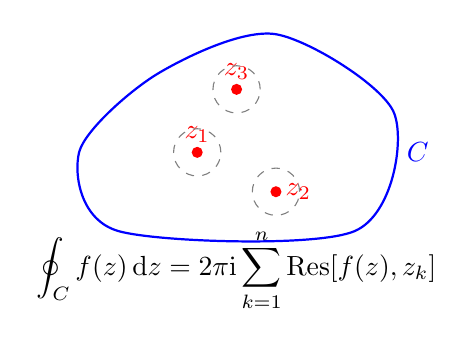
\begin{tikzpicture}[scale=1.0]
    \draw[blue, thick, ->] plot[smooth cycle] coordinates {(0,0) (3,0) (3.5,1.5) (2,2.5) (0.5,2) (-0.5,1)};
    \node[blue] at (3.8, 1) {$C$};

    \fill[red] (1, 1) circle (2pt) node[above] {$z_1$};
    \fill[red] (2, 0.5) circle (2pt) node[right] {$z_2$};
    \fill[red] (1.5, 1.8) circle (2pt) node[above] {$z_3$};

    \draw[gray, dashed] (1,1) circle (0.3);
    \draw[gray, dashed] (2,0.5) circle (0.3);
    \draw[gray, dashed] (1.5,1.8) circle (0.3);

    \node at (1.5,-0.5) {$\displaystyle \oint_C f(z)\,\mathrm{d}z = 2\pi \mathrm{i}\sum_{k=1}^n \operatorname{Res}[f(z),z_k]$};
\end{tikzpicture}
\caption{留数定理：整体闭路积分等于内部奇点的局部贡献之和}
\label{fig:residue-theorem}
\end{figure}

\begin{proof}
以每个奇点 $z_k$ 为圆心作一个足够小的圆 $C_k$，使这些小圆彼此互不相交，且都包含在 $D$ 内。把这些小圆盘从区域 $D$ 中挖去，得到一个多连通区域。由于所有奇点都已经被挖掉，所以 $f$ 在这个多连通区域内解析。

由多连通区域上的柯西积分定理，
\[
    \oint_C f(z)\,\mathrm{d}z
    =
    \sum_{k=1}^{n}\oint_{C_k} f(z)\,\mathrm{d}z.
\]
这里每个 $C_k$ 都取与外边界相适应的方向，故右边是各小围道积分之和。

又因为每个 $C_k$ 都只包围奇点 $z_k$，由上一节的小圆积分公式，
\[
    \oint_{C_k} f(z)\,\mathrm{d}z
    =
    2\pi \mathrm{i}\,\operatorname{Res}[f(z),z_k].
\]
把这些式子相加，就得到
\[
    \oint_C f(z)\,\mathrm{d}z
    =
    2\pi \mathrm{i}\sum_{k=1}^{n}\operatorname{Res}[f(z),z_k].
\]
\end{proof}

\begin{tishi}[留数定理真正重要在哪里]
留数定理把一个看起来属于\textbf{边界积分}的问题，转化成了若干个\textbf{局部系数}的代数求和问题。这就是它最核心的威力。以后你会越来越强烈地感受到：在复分析里，奇点附近的局部结构常常足以决定整体行为。
\end{tishi}

\subsection{留数定理的应用}

\begin{lizi}{多个奇点的闭路积分}{}
计算
\[
    \oint_{|z|=2}\frac{z+1}{z^2-1}\,\mathrm{d}z.
\]

\begin{jie}
先看奇点。由于
\[
    \frac{z+1}{z^2-1}
    =
    \frac{z+1}{(z-1)(z+1)},
\]
其中 $z=1$ 是真正的极点，而 $z=-1$ 处分子分母同为零，它其实是一个可去奇点。也就是说，延拓以后函数只在 $z=1$ 有一个简单极点。

因此围道 $|z|=2$ 内真正需要考虑的只有 $z=1$。

在 $z=1$ 处，
\[
    \operatorname{Res}\left[\frac{z+1}{z^2-1},1\right]
    =
    \lim_{z\to 1}(z-1)\frac{z+1}{(z-1)(z+1)}
    =1.
\]
于是由留数定理，
\[
    \oint_{|z|=2}\frac{z+1}{z^2-1}\,\mathrm{d}z
    =
    2\pi \mathrm{i}\cdot 1
    =
    2\pi \mathrm{i}.
\]
\end{jie}
\end{lizi}

\begin{lizi}{围道内外奇点的区别}{}
计算
\[
    \oint_{|z|=1}\frac{\mathrm{e}^z}{z(z-2)}\,\mathrm{d}z.
\]

\begin{jie}
函数的奇点为 $z=0$ 与 $z=2$。其中 $z=0$ 在圆 $|z|=1$ 内，而 $z=2$ 在圆外。

因此只需计算 $z=0$ 处的留数：
\[
    \operatorname{Res}\left[\frac{\mathrm{e}^z}{z(z-2)},0\right]
    =
    \lim_{z\to 0}
    z\cdot \frac{\mathrm{e}^z}{z(z-2)}
    =
    \lim_{z\to 0}\frac{\mathrm{e}^z}{z-2}
    =
    -\frac{1}{2}.
\]
于是
\[
    \oint_{|z|=1}\frac{\mathrm{e}^z}{z(z-2)}\,\mathrm{d}z
    =
    2\pi \mathrm{i}\cdot \left(-\frac{1}{2}\right)
    =
    -\pi \mathrm{i}.
\]
\end{jie}
\end{lizi}

\begin{jinshi}[一个必须先检查的条件]
使用留数定理前，首先要确认：\textbf{围道上不能有奇点。}如果奇点正好落在围道上，那么围道积分本身就需要重新解释，不能直接把留数定理硬套上去。
\end{jinshi}

\section{留数法计算积分的一般步骤}

\begin{wulibj}[本节的任务]
很多同学真正卡住的地方，不是在定理本身，而是在题目前：拿到一道积分题后，不知道该先找奇点、先选围道，还是先换元。本节不追求新公式，而是把留数法做题时最常见的判断流程整理出来。
\end{wulibj}

\begin{figure}[htbp]
\centering
\begin{tikzpicture}[
    node distance=0.75cm and 1.0cm,
    box/.style={rectangle, rounded corners=4pt, draw=blue!60!black, fill=blue!6, text width=3.1cm, minimum height=0.9cm, align=center, font=\small},
    arrow/.style={-{Stealth[length=2.3mm]}, thick, gray!75!black}
]
\node[box] (a) {先判断题型\\闭路积分、单位圆积分、无穷积分、振荡积分};
\node[box, below=of a] (b) {再找奇点\\位置、阶数、哪些在围道内};
\node[box, below=of b] (c) {再选围道\\单位圆、上半圆、下半圆或其他路径};
\node[box, below=of c] (d) {再算留数\\优先选最省力的方法};
\node[box, below=of d] (e) {再检查附加弧\\不能默认一定趋于零};
\node[box, below=of e] (f) {最后回到原积分\\注意实部、虚部、系数和方向};

\draw[arrow] (a) -- (b);
\draw[arrow] (b) -- (c);
\draw[arrow] (c) -- (d);
\draw[arrow] (d) -- (e);
\draw[arrow] (e) -- (f);
\end{tikzpicture}
\caption{留数法处理积分时的常见步骤}
\label{fig:residue-workflow}
\end{figure}

\subsection{先判断题目属于哪一类}

并不是所有积分题都要走同一条路线。通常至少要先分清下面几类：

\begin{enumerate}
    \item \textbf{闭路积分：}围道已经给定，此时重点是找出围道内部的奇点。
    \item \textbf{三角积分：}常见形状是
    \[
        \int_0^{2\pi} R(\cos\theta,\sin\theta)\,\mathrm{d}\theta,
    \]
    通常应想到单位圆代换 $z=\mathrm{e}^{\mathrm{i}\theta}$。
    \item \textbf{实轴无穷积分：}常见形状是
    \[
        \int_{-\infty}^{+\infty} R(x)\,\mathrm{d}x,
    \]
    常和大半圆围道有关。
    \item \textbf{带振荡因子的无穷积分：}例如
    \[
        \int_{-\infty}^{+\infty} R(x)\mathrm{e}^{\mathrm{i}ax}\,\mathrm{d}x,
    \]
    这时通常还要结合约当引理。
\end{enumerate}

\subsection{怎样找奇点与选围道}

题型判断清楚以后，下一步是找奇点，并思考它们与围道的位置关系。这里最容易忽略的是：\textbf{围道不是随便画的，它必须服务于原积分。}

\begin{itemize}
    \item 单位圆方法的围道不是猜出来的，而是由 $z=\mathrm{e}^{\mathrm{i}\theta}$ 这个换元自然给出的。
    \item 实轴无穷积分里常取上半圆或下半圆，但究竟选哪一侧，要看被积函数在那一侧是否更容易让附加弧积分消失。
    \item 若积分里出现 $\mathrm{e}^{\mathrm{i}ax}$，则上半平面还是下半平面的选择，通常由 $a$ 的符号决定。
\end{itemize}

\subsection{怎样检查附加路径积分}

留数法最容易被机械化的地方就在这里。很多人一看到半圆围道就默认``大圆弧积分一定趋于零''，这是很危险的。更稳妥的想法是：\textbf{先写估计，再判断是否真的趋于零。}

例如，对有理函数
\[
    R(z)=\frac{P(z)}{Q(z)},
\]
若分母次数比分子次数至少高 $2$，那么在大圆弧上往往有足够衰减；而若只高 $1$，就要更仔细地看。对含 $\mathrm{e}^{\mathrm{i}az}$ 的情形，则应额外利用指数因子在某个半平面的衰减。

\subsection{怎样把闭路积分还原成原积分}

复积分算完以后，还要回到原题。常见的回收方式有：

\begin{enumerate}
    \item \textbf{取实部或虚部：}很多 $\cos ax$、$\sin ax$ 型积分都要先转成 $\mathrm{e}^{\mathrm{i}ax}$，最后再取实部或虚部。
    \item \textbf{利用偶函数或奇函数：}例如
    \[
        \int_0^{+\infty}\frac{\cos x}{x^2+1}\,\mathrm{d}x
    \]
    常先补成整个实轴，再利用偶性除以 $2$。
    \item \textbf{注意换元带来的系数：}单位圆方法里
    \[
        \mathrm{d}\theta=\frac{\mathrm{d}z}{\mathrm{i}z},
    \]
    这个因子最容易漏。
\end{enumerate}

\begin{tishi}[把做题流程说成人话]
看到一道新题时，可以先问自己六个问题：
\begin{enumerate}
    \item 这是什么类型的积分？
    \item 它对应的复函数是什么？
    \item 奇点在哪里？
    \item 围道应该怎么选？
    \item 附加弧积分会不会消失？
    \item 最后该怎样回到原来的实积分？
\end{enumerate}
如果这六问都答得顺，留数法的思路一般就不会乱。
\end{tishi}

\begin{jinshi}[这一节最值得防的错误]
\begin{enumerate}
    \item 不要把``选围道''理解成背模板；围道必须和原积分结构匹配。
    \item 不要忘记检查附加弧积分。
    \item 不要在复积分算完后忘了回到原积分，尤其是取实部、取虚部和除以 $2$ 这几步。
\end{enumerate}
\end{jinshi}

\section{留数在实积分中的典型应用}

\begin{wulibj}[本节的任务]
前几节已经把工具准备好了。本节要真正展示留数理论的计算威力。为了让思路尽量顺畅，我们按难度递进来讲：先是单位圆方法处理三角积分，再是半圆围道处理有理型无穷积分，最后才是带振荡因子的积分与约当引理。
\end{wulibj}

\subsection{三角积分与单位圆方法}

考虑形如
\[
    \int_0^{2\pi} R(\cos\theta,\sin\theta)\,\mathrm{d}\theta
\]
的积分，其中 $R$ 是有理函数。最自然的换元是
\[
    z=\mathrm{e}^{\mathrm{i}\theta}.
\]
这样当 $\theta$ 从 $0$ 变到 $2\pi$ 时，$z$ 恰好沿单位圆逆时针走一周，并且
\[
    \cos\theta=\frac{z+z^{-1}}{2},\qquad
    \sin\theta=\frac{z-z^{-1}}{2\mathrm{i}},\qquad
    \mathrm{d}\theta=\frac{\mathrm{d}z}{\mathrm{i}z}.
\]

\begin{figure}[htbp]
\centering
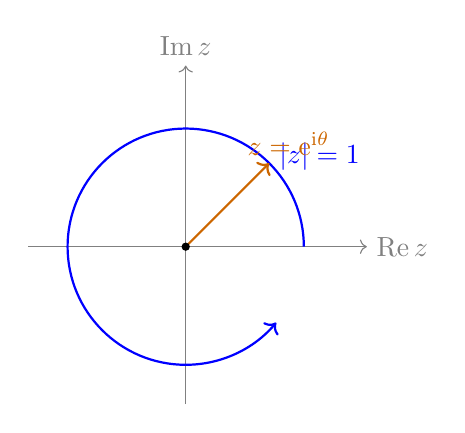
\begin{tikzpicture}[scale=1.0]
    \draw[->, gray] (-2,0) -- (2.3,0) node[right] {$\operatorname{Re} z$};
    \draw[->, gray] (0,-2) -- (0,2.3) node[above] {$\operatorname{Im} z$};
    \draw[blue, thick, ->] (1.5,0) arc[start angle=0,end angle=320,radius=1.5];
    \node[blue] at (1.7,1.15) {$|z|=1$};
    \draw[orange!80!black, thick, ->] (0,0) -- (45:1.5);
    \node[orange!80!black] at (45:1.85) {$z=\mathrm{e}^{\mathrm{i}\theta}$};
    \fill (0,0) circle (1.5pt);
\end{tikzpicture}
\caption{单位圆方法：$\theta$ 的积分转化为 $|z|=1$ 上的围道积分}
\label{fig:unit-circle-substitution}
\end{figure}

\begin{lizi}{单位圆方法的标准例题}{}
计算
\[
    I=\int_0^{2\pi}\frac{1}{1+a\cos\theta}\,\mathrm{d}\theta,
    \qquad 0<a<1.
\]

\begin{jie}
令 $z=\mathrm{e}^{\mathrm{i}\theta}$，则
\[
    \cos\theta=\frac{z+z^{-1}}{2},\qquad
    \mathrm{d}\theta=\frac{\mathrm{d}z}{\mathrm{i}z}.
\]
因此
\begin{align*}
    I
    &=
    \oint_{|z|=1}
    \frac{1}{1+\frac{a}{2}(z+z^{-1})}
    \cdot
    \frac{\mathrm{d}z}{\mathrm{i}z} \\
    &=
    \oint_{|z|=1}
    \frac{2\,\mathrm{d}z}{\mathrm{i}(az^2+2z+a)} \\
    &=
    \frac{2}{\mathrm{i}a}
    \oint_{|z|=1}
    \frac{\mathrm{d}z}{z^2+\frac{2}{a}z+1}.
\end{align*}

设
\[
    z^2+\frac{2}{a}z+1=0
\]
的两个根为 $z_1,z_2$。因为
\[
    z_1 z_2=1,
\]
所以这两个根中恰有一个在单位圆内。又由求根公式，
\[
    z_1-z_2=\frac{2\sqrt{1-a^2}}{a}.
\]
设 $z_1$ 为单位圆内的根，则被积函数在单位圆内只有一个简单极点 $z_1$，其留数为
\[
    \operatorname{Res}\left[\frac{1}{(z-z_1)(z-z_2)},z_1\right]
    =
    \frac{1}{z_1-z_2}.
\]
于是
\[
    I
    =
    \frac{2}{\mathrm{i}a}\cdot 2\pi \mathrm{i}\cdot \frac{1}{z_1-z_2}
    =
    \frac{4\pi}{a(z_1-z_2)}
    =
    \frac{2\pi}{\sqrt{1-a^2}}.
\]
\end{jie}
\end{lizi}

\begin{tishi}[单位圆方法的本质]
这类题的关键，并不只是记住
\[
    z=\mathrm{e}^{\mathrm{i}\theta}
\]
这个换元，而是意识到：它把三角函数问题改写成了\textbf{单位圆上的有理函数围道积分}。一旦改写完成，后面就是留数定理在工作。
\end{tishi}

\subsection{有理型无穷积分}

现在来看形如
\[
    \int_{-\infty}^{+\infty} R(x)\,\mathrm{d}x
\]
的积分，其中 $R$ 是有理函数。若分母次数比分子次数高得足够多，常见做法是在上半平面或下半平面补上一段大半圆，把实轴积分变成闭路积分。

\begin{figure}[htbp]
\centering
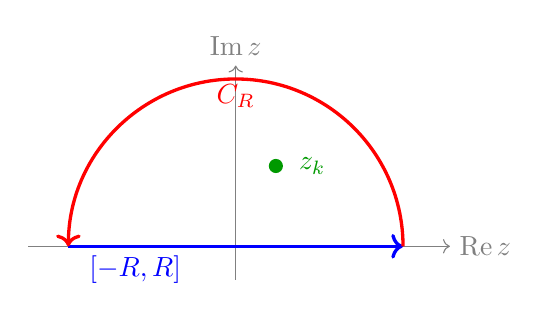
\begin{tikzpicture}[scale=0.85]
    \draw[->, gray] (-3.1,0) -- (3.2,0) node[right] {$\operatorname{Re} z$};
    \draw[->, gray] (0,-0.5) -- (0,2.7) node[above] {$\operatorname{Im} z$};

    \draw[blue, very thick, ->] (-2.5,0) -- (2.5,0);
    \draw[red, very thick, ->] (2.5,0) arc (0:180:2.5);
    \fill[green!60!black] (0.6,1.2) circle (3pt);
    \node[green!60!black, right] at (0.8,1.2) {$z_k$};
    \node[red] at (0,2.25) {$C_R$};
    \node[blue, below] at (-1.5,0) {$[-R,R]$};
\end{tikzpicture}
\caption{有理型无穷积分常用的上半平面围道}
\label{fig:upper-half-contour}
\end{figure}

\begin{lizi}{最标准的无穷积分}{}
计算
\[
    I=\int_{-\infty}^{+\infty}\frac{1}{x^2+a^2}\,\mathrm{d}x,
    \qquad a>0.
\]

\begin{jie}
取复函数
\[
    f(z)=\frac{1}{z^2+a^2}.
\]
它的极点是
\[
    z=\pm a\mathrm{i}.
\]
若取上半平面的半圆围道，则围道内部只有一个简单极点 $z=a\mathrm{i}$。

先计算该点的留数：
\[
    \operatorname{Res}[f(z),a\mathrm{i}]
    =
    \lim_{z\to a\mathrm{i}}
    \frac{z-a\mathrm{i}}{z^2+a^2}
    =
    \lim_{z\to a\mathrm{i}}
    \frac{1}{z+a\mathrm{i}}
    =
    \frac{1}{2a\mathrm{i}}.
\]

再看大半圆上的积分。设大半圆半径为 $R$，当 $R>a$ 时，在弧上有
\[
    |z^2+a^2|\ge |z|^2-a^2=R^2-a^2,
\]
因此
\[
    \left|\int_{C_R}\frac{1}{z^2+a^2}\,\mathrm{d}z\right|
    \le
    \frac{\pi R}{R^2-a^2}\to 0
    \qquad (R\to\infty).
\]
于是由留数定理，
\[
    I
    =
    2\pi \mathrm{i}\cdot \frac{1}{2a\mathrm{i}}
    =
    \frac{\pi}{a}.
\]
\end{jie}
\end{lizi}

\begin{lizi}{稍复杂的有理型无穷积分}{}
计算
\[
    I=\int_{-\infty}^{+\infty}\frac{x^2}{x^4+1}\,\mathrm{d}x.
\]

\begin{jie}
考虑
\[
    f(z)=\frac{z^2}{z^4+1}.
\]
方程
\[
    z^4+1=0
\]
的四个根是
\[
    \mathrm{e}^{\mathrm{i}\pi/4},\quad
    \mathrm{e}^{3\mathrm{i}\pi/4},\quad
    \mathrm{e}^{5\mathrm{i}\pi/4},\quad
    \mathrm{e}^{7\mathrm{i}\pi/4}.
\]
上半平面内的两个极点为
\[
    z_1=\mathrm{e}^{\mathrm{i}\pi/4},\qquad
    z_2=\mathrm{e}^{3\mathrm{i}\pi/4}.
\]

由于它们都是简单极点，而
\[
    (z^4+1)'=4z^3,
\]
所以
\[
    \operatorname{Res}[f(z),z_k]
    =
    \frac{z_k^2}{4z_k^3}
    =
    \frac{1}{4z_k}
    \qquad (k=1,2).
\]
因此
\[
    \operatorname{Res}[f(z),z_1]+\operatorname{Res}[f(z),z_2]
    =
    \frac{1}{4}\left(\frac{1}{z_1}+\frac{1}{z_2}\right).
\]
而
\[
    \frac{1}{z_1}=\mathrm{e}^{-\mathrm{i}\pi/4},\qquad
    \frac{1}{z_2}=\mathrm{e}^{-3\mathrm{i}\pi/4},
\]
故
\[
    \frac{1}{z_1}+\frac{1}{z_2}
    =
    \frac{1-\mathrm{i}}{\sqrt{2}}+\frac{-1-\mathrm{i}}{\sqrt{2}}
    =
    -\sqrt{2}\,\mathrm{i}.
\]
于是留数和为
\[
    -\frac{\mathrm{i}}{2\sqrt{2}}.
\]

再看大半圆上的积分。因为分母次数比分子次数高 $2$，与上一题同理，大圆弧上的积分趋于零。于是
\[
    I
    =
    2\pi \mathrm{i}\left(-\frac{\mathrm{i}}{2\sqrt{2}}\right)
    =
    \frac{\pi}{\sqrt{2}}.
\]
\end{jie}
\end{lizi}

\subsection{含振荡因子的无穷积分与约当引理}

当积分里出现
\[
    \mathrm{e}^{\mathrm{i}ax}
\]
这类振荡因子时，情况会比单纯的有理函数稍复杂一些。这里最核心的问题是：\textbf{大半圆弧上的积分为什么还能消失？}回答这个问题的常用工具就是约当引理。

\begin{dingli}{约当引理}{}
设 $f$ 在上半平面的充分大半圆及其内部除有限个点外解析，并且在半圆弧
\[
    C_R=\{z=R\mathrm{e}^{\mathrm{i}\theta}:0\le \theta\le \pi\}
\]
上满足
\[
    \max_{z\in C_R}|f(z)|\to 0
    \qquad (R\to\infty).
\]
则对任意 $a>0$，
\[
    \lim_{R\to\infty}\int_{C_R} f(z)\mathrm{e}^{\mathrm{i}az}\,\mathrm{d}z=0.
\]
\end{dingli}

\begin{figure}[htbp]
\centering
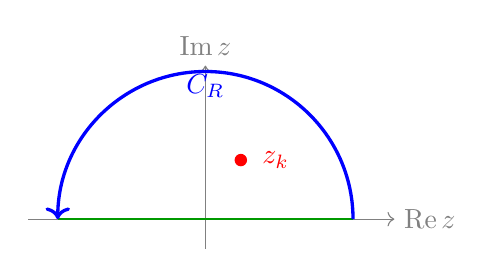
\begin{tikzpicture}[scale=0.75]
    \draw[->, gray] (-3.0,0) -- (3.2,0) node[right] {$\operatorname{Re} z$};
    \draw[->, gray] (0,-0.5) -- (0,2.6) node[above] {$\operatorname{Im} z$};

    \draw[green!60!black, thick] (-2.5,0) -- (2.5,0);
    \draw[blue, very thick, ->] (2.5,0) arc (0:180:2.5);
    \fill[red] (0.6,1.0) circle (3pt);
    \node[red, right] at (0.8,1.0) {$z_k$};
    \node[blue] at (0,2.25) {$C_R$};
\end{tikzpicture}
\caption{含 $\mathrm{e}^{\mathrm{i}az}$ 的积分常用围道}
\label{fig:jordan-contour-ch05}
\end{figure}

\begin{proof}
设
\[
    M_R=\max_{z\in C_R}|f(z)|.
\]
在半圆弧上令 $z=R\mathrm{e}^{\mathrm{i}\theta}$，则
\[
    \mathrm{d}z=\mathrm{i}R\mathrm{e}^{\mathrm{i}\theta}\,\mathrm{d}\theta,
    \qquad 0\le \theta\le \pi.
\]
又因为
\[
    \left|\mathrm{e}^{\mathrm{i}az}\right|
    =
    \left|\mathrm{e}^{\mathrm{i}aR(\cos\theta+\mathrm{i}\sin\theta)}\right|
    =
    \mathrm{e}^{-aR\sin\theta},
\]
所以
\[
    \left|\int_{C_R} f(z)\mathrm{e}^{\mathrm{i}az}\,\mathrm{d}z\right|
    \le
    M_R R\int_0^\pi \mathrm{e}^{-aR\sin\theta}\,\mathrm{d}\theta.
\]
而标准估计给出
\[
    \int_0^\pi \mathrm{e}^{-aR\sin\theta}\,\mathrm{d}\theta
    \le
    \frac{\pi}{aR}.
\]
于是
\[
    \left|\int_{C_R} f(z)\mathrm{e}^{\mathrm{i}az}\,\mathrm{d}z\right|
    \le
    \frac{\pi M_R}{a}\to 0.
\]
故结论成立。
\end{proof}

\begin{lizi}{由复指数转回余弦积分}{}
计算
\[
    I=\int_0^{+\infty}\frac{\cos x}{x^2+1}\,\mathrm{d}x.
\]

\begin{jie}
先考虑整个实轴上的复积分
\[
    J=\int_{-\infty}^{+\infty}\frac{\mathrm{e}^{\mathrm{i}x}}{x^2+1}\,\mathrm{d}x.
\]
取复函数
\[
    f(z)=\frac{\mathrm{e}^{\mathrm{i}z}}{z^2+1},
\]
并在上半平面闭合围道。因为 $a=1>0$，指数因子在上半平面有衰减，所以可用约当引理说明大圆弧上的积分趋于零。

围道内部只有一个简单极点 $z=\mathrm{i}$。其留数为
\[
    \operatorname{Res}[f(z),\mathrm{i}]
    =
    \lim_{z\to \mathrm{i}}
    \frac{(z-\mathrm{i})\mathrm{e}^{\mathrm{i}z}}{(z-\mathrm{i})(z+\mathrm{i})}
    =
    \frac{\mathrm{e}^{\mathrm{i}\cdot \mathrm{i}}}{2\mathrm{i}}
    =
    \frac{\mathrm{e}^{-1}}{2\mathrm{i}}.
\]
因此
\[
    J
    =
    2\pi \mathrm{i}\cdot \frac{\mathrm{e}^{-1}}{2\mathrm{i}}
    =
    \frac{\pi}{\mathrm{e}}.
\]

另一方面，
\[
    J
    =
    \int_{-\infty}^{+\infty}\frac{\cos x}{x^2+1}\,\mathrm{d}x
    +
    \mathrm{i}
    \int_{-\infty}^{+\infty}\frac{\sin x}{x^2+1}\,\mathrm{d}x.
\]
其中虚部对应的积分是奇函数在对称区间上的积分，因此为零，所以
\[
    \int_{-\infty}^{+\infty}\frac{\cos x}{x^2+1}\,\mathrm{d}x
    =
    \frac{\pi}{\mathrm{e}}.
\]
又因为被积函数是偶函数，于是
\[
    I
    =
    \frac{1}{2}\cdot \frac{\pi}{\mathrm{e}}
    =
    \frac{\pi}{2\mathrm{e}}.
\]
\end{jie}
\end{lizi}

\begin{lizi}{由复指数转回正弦积分}{}
计算
\[
    I=\int_0^{+\infty}\frac{x\sin x}{x^2+1}\,\mathrm{d}x.
\]

\begin{jie}
考虑
\[
    J=\int_{-\infty}^{+\infty}\frac{x\mathrm{e}^{\mathrm{i}x}}{x^2+1}\,\mathrm{d}x.
\]
取
\[
    f(z)=\frac{z\mathrm{e}^{\mathrm{i}z}}{z^2+1}.
\]
与上一题同理，取上半平面围道，大圆弧积分由约当引理趋于零。

围道内部仍只有极点 $z=\mathrm{i}$。其留数为
\[
    \operatorname{Res}[f(z),\mathrm{i}]
    =
    \lim_{z\to \mathrm{i}}
    \frac{z\mathrm{e}^{\mathrm{i}z}}{z+\mathrm{i}}
    =
    \frac{\mathrm{i}\mathrm{e}^{-1}}{2\mathrm{i}}
    =
    \frac{\mathrm{e}^{-1}}{2}.
\]
因此
\[
    J=2\pi \mathrm{i}\cdot \frac{\mathrm{e}^{-1}}{2}
    =
    \frac{\pi \mathrm{i}}{\mathrm{e}}.
\]

再把 $J$ 拆成实部和虚部：
\[
    J
    =
    \int_{-\infty}^{+\infty}\frac{x\cos x}{x^2+1}\,\mathrm{d}x
    +
    \mathrm{i}
    \int_{-\infty}^{+\infty}\frac{x\sin x}{x^2+1}\,\mathrm{d}x.
\]
其中第一项是奇函数在对称区间上的积分，因此为零。所以
\[
    \int_{-\infty}^{+\infty}\frac{x\sin x}{x^2+1}\,\mathrm{d}x
    =
    \frac{\pi}{\mathrm{e}}.
\]
而
\[
    \frac{x\sin x}{x^2+1}
\]
是偶函数，因此
\[
    I
    =
    \frac{1}{2}\cdot \frac{\pi}{\mathrm{e}}
    =
    \frac{\pi}{2\mathrm{e}}.
\]
\end{jie}
\end{lizi}

\section{对数留数、辐角原理与鲁歇定理（选读）}

\begin{wulibj}[本节的任务]
前面几节强调的是留数在\textbf{积分计算}中的作用；本节则想让学生进一步看到，留数还可以用来研究\textbf{零点和极点的个数}。关键对象是
\[
    \frac{f'(z)}{f(z)}.
\]
它会把零点和极点的重数直接转化为留数，于是``数根问题''也就可以转化为积分问题。
\end{wulibj}

\begin{tishi}[选读说明]
这一节在逻辑上和前面的主线是连着的，但学习重心已经从``算积分''转向``数零点''。如果课程重点更偏计算应用，可以把这一节作为选读；如果后面准备进一步讲映射理论，那么这一节就会成为非常重要的桥梁。
\end{tishi}

\subsection{\texorpdfstring{为什么考虑 $f'(z)/f(z)$}{为什么考虑 f'(z)/f(z)}}

如果我们想知道某个区域里有多少个零点和极点，最自然的想法是：找一个函数，它在零点和极点附近能把``重数''直接暴露出来。对数导数
\[
    \frac{f'(z)}{f(z)}
\]
恰好就有这种性质。

\begin{dingli}{\texorpdfstring{$f'(z)/f(z)$}{f'(z)/f(z)} 在零点与极点处的留数}{}
设 $z_0$ 是 $f$ 的孤立零点或孤立极点。
\begin{enumerate}
    \item 若 $z_0$ 是 $f$ 的 $m$ 阶零点，则
    \[
        \operatorname{Res}\left[\frac{f'(z)}{f(z)},z_0\right]=m.
    \]
    \item 若 $z_0$ 是 $f$ 的 $m$ 阶极点，则
    \[
        \operatorname{Res}\left[\frac{f'(z)}{f(z)},z_0\right]=-m.
    \]
\end{enumerate}
\end{dingli}

\begin{proof}
先设 $z_0$ 是 $f$ 的 $m$ 阶零点，则可写成
\[
    f(z)=(z-z_0)^m g(z),
\]
其中 $g$ 在 $z_0$ 附近解析且 $g(z_0)\neq 0$。对两边求导并除以 $f(z)$，得
\[
    \frac{f'(z)}{f(z)}
    =
    \frac{m}{z-z_0}+\frac{g'(z)}{g(z)}.
\]
第二项在 $z_0$ 附近解析，所以其留数为零。因此
\[
    \operatorname{Res}\left[\frac{f'(z)}{f(z)},z_0\right]=m.
\]

若 $z_0$ 是 $m$ 阶极点，则可写成
\[
    f(z)=\frac{g(z)}{(z-z_0)^m},
\]
其中 $g$ 在 $z_0$ 附近解析且 $g(z_0)\neq 0$。于是
\[
    \frac{f'(z)}{f(z)}
    =
    \frac{g'(z)}{g(z)}-\frac{m}{z-z_0},
\]
所以对应留数为 $-m$。
\end{proof}

\subsection{对数留数与辐角原理}

\begin{dingliyi}{对数留数}{}
设 $f$ 在简单闭曲线 $C$ 上不为零，并且在 $C$ 的内部只有有限个零点和极点，则
\[
    \frac{1}{2\pi \mathrm{i}}\oint_C \frac{f'(z)}{f(z)}\,\mathrm{d}z
\]
称为 $f$ 关于曲线 $C$ 的\textbf{对数留数}。
\end{dingliyi}

\begin{dingli}{辐角原理}{}
设 $f$ 在简单闭曲线 $C$ 上解析且不为零，在 $C$ 内部有 $N$ 个零点和 $P$ 个极点，均按重数计，则
\[
    \frac{1}{2\pi \mathrm{i}}
    \oint_C \frac{f'(z)}{f(z)}\,\mathrm{d}z
    =
    N-P.
\]
\end{dingli}

\begin{proof}
由上一条定理可知，函数
\[
    \frac{f'(z)}{f(z)}
\]
在 $f$ 的每个零点和极点处都有简单极点，而且留数分别是相应零点重数和极点重数的相反数。因此由留数定理，
\[
    \oint_C \frac{f'(z)}{f(z)}\,\mathrm{d}z
    =
    2\pi \mathrm{i}(N-P).
\]
两边再除以 $2\pi \mathrm{i}$，便得到结论。
\end{proof}

\begin{tishi}[辐角原理的几何意义]
当 $z$ 沿曲线 $C$ 走一周时，像点 $w=f(z)$ 也会在像平面中走出一条闭曲线。辐角原理说明：这条像曲线绕原点的圈数，正好等于 $C$ 内部零点总重数减去极点总重数。
\end{tishi}

\subsection{鲁歇定理}

\begin{dingli}{鲁歇定理}{}
设 $f$ 和 $g$ 在简单闭曲线 $C$ 上及其内部解析，并且在 $C$ 上满足
\[
    |f(z)|>|g(z)|,
\]
则 $f$ 与 $f+g$ 在 $C$ 内部有相同个数的零点，按重数计。
\end{dingli}

\begin{proof}
考虑一族函数
\[
    h_t(z)=f(z)+tg(z),\qquad 0\le t\le 1.
\]
在曲线 $C$ 上，由条件
\[
    |h_t(z)|
    \ge |f(z)|-t|g(z)|
    \ge |f(z)|-|g(z)|
    >0,
\]
所以对所有 $t\in[0,1]$，$h_t$ 在 $C$ 上都不为零。

于是由辐角原理，
\[
    N(t)=\frac{1}{2\pi \mathrm{i}}\oint_C \frac{h_t'(z)}{h_t(z)}\,\mathrm{d}z
\]
给出 $h_t$ 在 $C$ 内的零点个数。由于积分关于 $t$ 连续变化，而 $N(t)$ 只能取整数值，所以 $N(t)$ 必为常数。

当 $t=0$ 时，$h_t=f$；当 $t=1$ 时，$h_t=f+g$。因此二者在 $C$ 内部的零点个数相同。
\end{proof}

\begin{lizi}{用鲁歇定理数根}{}
证明方程
\[
    z^8-5z^5-2z+1=0
\]
在单位圆内有 $5$ 个根。

\begin{jie}
在单位圆 $|z|=1$ 上取
\[
    f(z)=-5z^5,\qquad g(z)=z^8-2z+1.
\]
则
\[
    |f(z)|=5,
\]
而
\[
    |g(z)|\le |z|^8+2|z|+1=1+2+1=4.
\]
因此在单位圆上有
\[
    |f(z)|>|g(z)|.
\]
由鲁歇定理，$f$ 与 $f+g=z^8-5z^5-2z+1$ 在单位圆内有相同数目的零点。

而
\[
    f(z)=-5z^5
\]
在单位圆内只有一个零点 $z=0$，但它是 $5$ 重零点，所以零点总数按重数计为 $5$。因此原方程在单位圆内有 $5$ 个根。
\end{jie}
\end{lizi}

\section{本章小结}

\begin{tishi}[一句话回看本章]
本章最核心的事情，是把奇点附近的局部展开进一步压缩成一个关键系数，并说明这个系数怎样控制闭路积分、实积分，乃至零点与极点的计数。换句话说，本章真正建立起来的，是``局部信息如何进入整体计算''的眼光。
\end{tishi}

\begin{figure}[htbp]
\centering
\begin{tikzpicture}[
    node distance=1.0cm and 1.8cm,
    concept/.style={rectangle, rounded corners=4pt, draw=blue!60!black, fill=blue!6, text width=3.3cm, minimum height=0.85cm, align=center, font=\small},
    result/.style={rectangle, rounded corners=4pt, draw=green!60!black, fill=green!8, text width=3.4cm, minimum height=0.85cm, align=center, font=\small},
    arrow/.style={-{Stealth[length=2.4mm]}, thick, gray!75!black}
]
\node[concept] (laurent) {洛朗展开\\负幂项记录奇点结构};
\node[result, below=of laurent] (res) {$c_{-1}$ 的特殊地位\\$\Longrightarrow$ 留数};
\node[concept, below left=1.2cm and 0.8cm of res] (thm) {留数定理\\局部系数控制整体积分};
\node[concept, below right=1.2cm and 0.8cm of res] (calc) {实积分应用\\单位圆方法、半圆围道、约当引理};
\node[result, below=1.2cm of res] (count) {$\dfrac{f'}{f}$ 的留数\\$\Longrightarrow$ 零点与极点计数};

\draw[arrow] (laurent) -- (res);
\draw[arrow] (res) -- (thm);
\draw[arrow] (res) -- (calc);
\draw[arrow] (thm) -- (count);
\draw[arrow] (calc) -- (count);
\end{tikzpicture}
\caption{本章知识主线：从局部系数走向整体积分与零点计数}
\label{fig:ch05-knowledge-map}
\end{figure}

\begin{zhongyao}[本章主要结论]
\raggedright
\begin{enumerate}
    \item \textbf{留数就是洛朗展开中的 $c_{-1}$：}它不是附加记号，而是被围道积分自动筛选出来的那一个特殊系数。
    \item \textbf{小圆积分只留下留数项：}若围绕孤立奇点作小圆积分，则
    \[
        \oint f(z)\,\mathrm{d}z = 2\pi \mathrm{i}\,\operatorname{Res}.
    \]
    这说明围道积分对局部展开有非常强的选择性。
    \item \textbf{留数定理把闭路积分化成局部贡献之和：}对有限个孤立奇点，整体闭路积分等于内部各点留数总和乘上 $2\pi \mathrm{i}$。
    \item \textbf{求留数时应先分类、再选法：}简单极点优先极限法或 $\dfrac{P(z_0)}{Q'(z_0)}$，高阶极点再考虑导数公式，容易展开的函数则可直接读洛朗展开。
    \item \textbf{留数法处理实积分时，围道选择是核心：}三角积分常转到单位圆上；有理型无穷积分常用大半圆围道；带振荡因子的积分则要结合约当引理。
    \item \textbf{$\dfrac{f'}{f}$ 的留数能读出零点与极点的重数：}这使留数理论自然延伸到辐角原理与鲁歇定理。
\end{enumerate}
\end{zhongyao}

\begin{tishi}[做题时的判断思路]
\begin{enumerate}
    \item 看到奇点问题，先问自己：要找的是奇点类型、主部，还是留数？
    \item 看到``求留数''，先判断该点是简单极点还是高阶极点，再决定是用极限法、快捷公式、导数公式，还是直接展开。
    \item 看到闭路积分，先数清围道内部到底有哪些奇点，不要把围道外的点也算进去。
    \item 看到三角积分，优先想到 $z=\mathrm{e}^{\mathrm{i}\theta}$。
    \item 看到实轴无穷积分，先问附加弧积分是否真的趋于零。
    \item 看到零点个数问题，则应想到 $\dfrac{f'}{f}$、辐角原理或鲁歇定理。
\end{enumerate}
\end{tishi}

\begin{jinshi}[本章最容易混淆的地方]
\begin{enumerate}
    \item 不要把留数看成奇点的全部信息；它只是主部里最特殊的那一项系数。
    \item 不要把``留数为零''误读成``该点解析''。
    \item 不要忘记留数定理要求围道上没有奇点。
    \item 不要做实积分时只顾求留数，而忘了检查附加弧积分和回收原积分。
    \item 不要在辐角原理和鲁歇定理里忘记``按重数计''这几个字。
\end{enumerate}
\end{jinshi}

\begin{tishi}[和前后内容的联系]
回头看，本章并不是凭空开始的。第四章最后通过洛朗展开说明了一阶负幂项的特殊地位，本章只是把这一观察正式提升为留数概念，并把它发展成留数定理。换句话说，本章的根扎在上一章的局部展开理论里。

往后看，本章的围道积分技巧会在傅里叶变换、拉普拉斯逆变换等内容中反复出现；而本章末尾的辐角原理和鲁歇定理，又会把学生带向更整体、更几何的复分析视角。所以留数理论恰好站在``局部展开''、``积分计算''和``零点分布''三条线的交汇处，是整段复变函数内容中承上启下的一章。
\end{tishi}

\section{习题}

\subsection*{基础题}

\begin{enumerate}
    \item 求下列函数在指定点处的留数：
    \begin{enumerate}
        \item $\displaystyle f(z)=\frac{z}{z^2+1},\quad z=\mathrm{i}$；
        \item $\displaystyle f(z)=\frac{1}{(z-1)^3},\quad z=1$；
        \item $\displaystyle f(z)=\frac{\mathrm{e}^z}{z(z-1)},\quad z=0,1$。
    \end{enumerate}

    \item 用留数定理计算：
    \begin{enumerate}
        \item $\displaystyle \oint_{|z|=2}\frac{z}{z^2-1}\,\mathrm{d}z$；
        \item $\displaystyle \oint_{|z|=1}\frac{\sin z}{z}\,\mathrm{d}z$。
    \end{enumerate}

    \item 判断下列说法是否正确，并说明理由：
    \begin{enumerate}
        \item 留数为零的点一定不是奇点；
        \item 围道内部奇点越多，闭路积分一定越大；
        \item 高阶极点的留数一定非零。
    \end{enumerate}
\end{enumerate}

\subsection*{综合题}

\begin{enumerate}
    \item 计算下列实积分：
    \begin{enumerate}
        \item $\displaystyle \int_0^{2\pi}\frac{1}{2+\cos\theta}\,\mathrm{d}\theta$；
        \item $\displaystyle \int_{-\infty}^{+\infty}\frac{x^2}{x^4+1}\,\mathrm{d}x$；
        \item $\displaystyle \int_0^{+\infty}\frac{x\sin x}{x^2+1}\,\mathrm{d}x$。
    \end{enumerate}

    \item 设
    \[
        f(z)=\frac{z^2+3z+1}{(z-1)^2(z+1)},
    \]
    求它在各个有限奇点处的留数，并计算
    \[
        \oint_{|z|=2} f(z)\,\mathrm{d}z.
    \]

    \item 用辐角原理说明：若 $f$ 在简单闭曲线 $C$ 上不为零，则
    \[
        \frac{1}{2\pi \mathrm{i}}\oint_C \frac{f'(z)}{f(z)}\,\mathrm{d}z
    \]
    一定是整数。
\end{enumerate}

\subsection*{挑战题}

\begin{enumerate}
    \item 证明：当 $a>|b|>0$ 时，
    \[
        \int_0^{2\pi}\frac{1}{a+b\cos\theta}\,\mathrm{d}\theta
        =
        \frac{2\pi}{\sqrt{a^2-b^2}}.
    \]

    \item 用鲁歇定理证明：方程
    \[
        z^5-z+1=0
    \]
    在单位圆内有 $1$ 个根。

    \item 设 $f$ 在简单闭曲线 $C$ 上及其内部解析，且在 $C$ 上满足
    \[
        |f(z)-z^n|<|z|^n.
    \]
    证明 $f$ 在 $C$ 内部有与 $z^n$ 相同数目的零点。
\end{enumerate}

%% 第六章：多值函数、支点与解析支（选学）

\chapter{多值函数、支点与解析支（选学）}

\begin{wulibj}[本章定位]
前五章里，我们讨论的主角基本都是单值解析函数：在给定区域里，每个 $z$ 都对应唯一的函数值，围绕解析性、级数展开和留数理论展开的一整套方法，也都是在这样的对象上建立起来的。

但当学生继续往前走时，很快就会遇到几个看似熟悉、其实又很不一样的对象：$\arg z$、$\log z$、$z^\alpha$、$\sqrt[n]{z}$。这些函数并不是简单地``再多记几个公式''就能处理，因为它们最根本的困难在于：\textbf{它们往往不能在整个区域里同时保持单值。}

因此，本章真正要解决的问题，不是``介绍几个特殊函数''，而是帮助学生理解：
\begin{enumerate}
    \item 多值性到底从哪里来；
    \item 为什么要引入主值、分支与支割；
    \item 怎样把一个多值对象放到合适的区域上，当作单值解析函数来处理；
    \item 为什么带多值函数的复积分题，往往必须先选支，再谈路径。
\end{enumerate}

从课程主线看，这一章一头连着前面的留数理论，一头又连着后面的保角映射与某些典型积分应用。它虽然标为选学，但对想真正把复变函数学明白的同学来说，是非常值得认真读的一章。
\end{wulibj}

\begin{tishi}[写作总原则]
\begin{enumerate}
    \item 本章应始终从``为什么会多值''讲起，而不要一上来就堆定义。
    \item 要反复把本章和第二章的``单连通区域''、第五章的``围道积分''联系起来。
    \item 黎曼面只保留直观说明，不展开成抽象理论主线。
    \item 例题应优先服务于理解支、支点、支割和积分路径的关系，而不是单纯追求技巧性。
    \item 图示要多，尤其要帮助学生看清``绕一圈为什么会变值''、``支割为什么要这样取''、``钥匙孔围道为什么长这样''。
\end{enumerate}
\end{tishi}

\section{多值现象的出现：从辐角谈起}

\begin{wulibj}[本节要解决的问题]
学生第一次接触多值函数时，最容易把它理解成``定义写得不够严谨''。本节的任务，就是先把这个误解消掉。我们要让学生看到：多值性不是书写上的漏洞，而是复平面几何结构带来的客观现象，而最自然的入口就是辐角。
\end{wulibj}

\subsection*{教学目标}
\begin{itemize}
    \item 让学生回顾复数的极形式，并重新认识辐角并不唯一这一事实。
    \item 让学生区分多值辐角 $\arg z$ 与主辐角 $\operatorname{Arg} z$。
    \item 让学生理解``绕原点一圈，角度多出 $2\pi$''是后面一切多值现象的起点。
\end{itemize}

\subsection*{建议小节安排}
\begin{enumerate}
    \item 从极形式重新看复数的表示
    \item 辐角为什么天然多值
    \item 主辐角的引入与局限
    \item 绕原点一圈时辐角如何变化
\end{enumerate}

\subsection*{本节必须讲清的核心点}
\begin{itemize}
    \item 对任意 $z\neq 0$，若
    \[
        z = r\mathrm{e}^{\mathrm{i}\theta},
    \]
    则
    \[
        \arg z = \theta + 2k\pi,\qquad k\in\mathbb{Z}.
    \]
    这里的多值性不是附加出来的，而是极形式本身就带有的。
    \item 主辐角 $\operatorname{Arg} z$ 只是从全部可能值中人为选出的一个代表值，常取
    \[
        -\pi < \operatorname{Arg} z \le \pi.
    \]
    \item 一旦沿着绕原点的闭路走一圈，辐角就会整体增加 $2\pi$，这正是后面 $\log z$ 与 $z^\alpha$ 多值性的根源。
    \item 原点之所以特殊，不是因为它函数值算不出来，而是因为``绕原点''会导致角度结构发生根本变化。
\end{itemize}

\subsection*{建议例题}
\begin{lizi}{辐角与主辐角}{}
写出 $1$、$-1$、$\mathrm{i}$、$-1+\mathrm{i}$ 的全部辐角与主辐角，并比较它们之间的区别。
\end{lizi}

\begin{lizi}{绕行导致辐角改变}{}
设 $z=\mathrm{e}^{\mathrm{i}\theta}$ 沿单位圆逆时针转一周，说明为什么起点与终点虽然对应同一个复数，但辐角却增加了 $2\pi$。
\end{lizi}

\subsection*{建议图示}
\begin{itemize}
    \item 复平面上一点对应多组辐角的示意图。
    \item 单位圆绕行一周时参数 $\theta$ 连续增加的示意图。
    \item 主辐角取值区间与负实轴跳变位置的示意图。
\end{itemize}

\begin{jinshi}[本节易错点]
\begin{enumerate}
    \item 不要把 $\arg z$ 和 $\operatorname{Arg} z$ 混为一谈。
    \item 不要以为主辐角是``唯一正确的辐角''；它只是常用的一种选法。
    \item 不要忽略原点在整个多值理论中的特殊地位。
\end{enumerate}
\end{jinshi}

\section{复对数函数与主值}

\begin{wulibj}[本节要解决的问题]
有了上一节的铺垫以后，学生会自然追问：如果辐角已经是多值的，那么由极形式定义出来的复对数会发生什么？本节的任务，就是让学生看到：复对数不是实对数的直接照搬，而是复分析中最基本、最典型的多值函数。
\end{wulibj}

\subsection*{教学目标}
\begin{itemize}
    \item 让学生掌握复对数的定义来源。
    \item 让学生理解 $\log z$ 与 $\operatorname{Log} z$ 的区别。
    \item 让学生意识到主值对数虽然是单值写法，但它只能在合适区域上讨论。
\end{itemize}

\subsection*{建议小节安排}
\begin{enumerate}
    \item 从 $z=r\mathrm{e}^{\mathrm{i}\theta}$ 出发定义 $\log z$
    \item 复对数的全部值
    \item 主值对数 $\operatorname{Log} z$
    \item 主值为什么会在支割处失去连续性
\end{enumerate}

\subsection*{本节必须讲清的核心点}
\begin{itemize}
    \item 复对数定义为
    \[
        \log z = \ln|z| + \mathrm{i}\arg z.
    \]
    因为 $\arg z$ 多值，所以 $\log z$ 也多值。
    \item 若取主辐角，则得到主值对数
    \[
        \operatorname{Log} z = \ln|z| + \mathrm{i}\operatorname{Arg} z.
    \]
    \item $\operatorname{Log} z$ 只是选定某一支后的写法，不等于``真正的复对数只有一个值''。
    \item 只要辐角在某条射线两侧发生跳变，主值对数在那条射线附近就不能保持连续，这也就预示了后面必须讨论支割。
\end{itemize}

\subsection*{建议例题}
\begin{lizi}{复对数的全部值}{}
求 $\log 1$、$\log(-1)$ 与 $\log \mathrm{i}$ 的全部值，并写出各自的主值。
\end{lizi}

\begin{lizi}{主值对数的连续性问题}{}
说明为什么当 $z$ 从负实轴上方和下方逼近同一点时，$\operatorname{Log} z$ 的极限一般不同。
\end{lizi}

\subsection*{建议图示}
\begin{itemize}
    \item 以负实轴为支割时，$\operatorname{Log} z$ 的定义区域示意图。
    \item 负实轴上下两侧主辐角取值突变的示意图。
\end{itemize}

\begin{jinshi}[本节易错点]
\begin{enumerate}
    \item 不要把 $\log z$ 和 $\operatorname{Log} z$ 混为一谈。
    \item 不要以为写下主值以后，函数就在整个去心平面上自动解析。
    \item 不要忘记复对数的多值性本质上来自辐角，而不是来自模长。
\end{enumerate}
\end{jinshi}

\section{分支、解析支与支割}

\begin{wulibj}[本节要解决的问题]
前两节已经告诉我们：有些复函数天然多值。接下来最关键的问题是：既然它本来多值，我们怎样在某个合适区域上把它固定成单值对象，并继续用解析函数的方法处理它？这一节就是全章的概念核心。
\end{wulibj}

\subsection*{教学目标}
\begin{itemize}
    \item 让学生理解什么叫一支、什么叫解析支。
    \item 让学生理解支割不是装饰性的几何线，而是为了让函数在剩余区域上单值解析。
    \item 让学生把本章和第二章的``单连通区域''重新联系起来。
\end{itemize}

\subsection*{建议小节安排}
\begin{enumerate}
    \item 从主值对数重新理解``选一支''
    \item 一般多值函数的一支与解析支
    \item 支割的作用与选择
    \item 单连通区域与解析支的关系
\end{enumerate}

\subsection*{本节必须讲清的核心点}
\begin{itemize}
    \item 所谓一支，就是从多值函数的全部可能值中，在某个区域上按一致规则选出一个单值函数。
    \item 所谓解析支，不只是选成单值，还要求该单值函数在所讨论区域里解析。
    \item 支一定依赖于定义域。离开具体区域，空谈``这个函数的支''是不完整的。
    \item 支割的作用，是把原来会因为绕行而变值的区域切开，使剩余区域尽量成为可以选取解析支的区域。
    \item 第二章中的``单连通''在这里重新变得重要，因为很多多值问题的困难，本质上正来自于区域中允许绕支点转一圈。
\end{itemize}

\subsection*{建议例题}
\begin{lizi}{不同支割对应不同支}{}
分别在去掉负实轴与去掉正实轴的区域上，为 $\log z$ 写出一个解析支，并比较它们的差异。
\end{lizi}

\begin{lizi}{为什么必须说明区域}{}
说明为什么不能说``$\log z$ 有一个全局解析支''，而只能说``在某个去掉射线的区域上可以选出解析支''。
\end{lizi}

\subsection*{建议图示}
\begin{itemize}
    \item 负实轴支割、正实轴支割与一般射线支割的对比图。
    \item 切开前后区域拓扑结构变化的示意图。
\end{itemize}

\begin{jinshi}[本节易错点]
\begin{enumerate}
    \item 不要把``支''理解成函数自己天然带着的一部分。
    \item 不要把支割理解成唯一标准答案；它通常有多种合理选择。
    \item 不要忽略``解析支''里的``解析''二字，它比单纯单值更强。
\end{enumerate}
\end{jinshi}

\section{典型多值函数：幂函数与根式函数}

\begin{wulibj}[本节要解决的问题]
学生学到这里，最需要建立的是统一观点：很多看起来各不相同的多值函数，其实都源于复对数。本节就要把 $\log z$、$z^\alpha$ 和 $\sqrt[n]{z}$ 这几类最重要的例子串起来。
\end{wulibj}

\subsection*{教学目标}
\begin{itemize}
    \item 让学生理解 $z^\alpha$ 的定义为什么离不开 $\log z$。
    \item 让学生理解整数幂、分数幂和无理幂在多值性上的区别。
    \item 让学生掌握 $\sqrt[n]{z}$ 的常见分支与几何意义。
\end{itemize}

\subsection*{建议小节安排}
\begin{enumerate}
    \item 复幂函数 $z^\alpha = \mathrm{e}^{\alpha \log z}$
    \item $\alpha$ 取不同类型值时的多值差异
    \item 根式函数 $\sqrt[n]{z}$ 的分支
    \item 主值根式与几何直观
\end{enumerate}

\subsection*{本节必须讲清的核心点}
\begin{itemize}
    \item 复幂函数定义为
    \[
        z^\alpha = \mathrm{e}^{\alpha \log z},
    \]
    因此它的多值性直接继承自 $\log z$。
    \item 当 $\alpha$ 为整数时，$z^\alpha$ 退化成熟悉的单值函数；当 $\alpha$ 为非整数时，多值性一般无法避免。
    \item 根式函数
    \[
        \sqrt[n]{z}=z^{1/n}
    \]
    是最适合帮助学生建立直观的一类对象，应重点讲清楚。
    \item 主值根式的选法，本质上也是先选定对数的一支，再把它代入幂函数定义。
\end{itemize}

\subsection*{建议例题}
\begin{lizi}{平方根的主值支}{}
在去掉负实轴的区域上写出 $\sqrt{z}$ 的主值支，并说明它为什么在该区域上解析。
\end{lizi}

\begin{lizi}{幂函数的全部值}{}
求 $(-1)^{1/2}$、$(-1)^{1/3}$ 与 $\mathrm{i}^{1/2}$ 的全部值，并比较它们的分支结构。
\end{lizi}

\begin{lizi}{不同指数导致不同多值性}{}
比较 $z^2$、$z^{1/2}$ 与 $z^{\sqrt{2}}$ 的多值行为，说明它们为什么性质差异很大。
\end{lizi}

\subsection*{建议图示}
\begin{itemize}
    \item $z^{1/2}$ 将辐角减半的示意图。
    \item $\sqrt{z}$ 的两叶直观图。
    \item $\sqrt[n]{z}$ 与 $z^n$ 在角度映射上的对比图。
\end{itemize}

\begin{jinshi}[本节易错点]
\begin{enumerate}
    \item 不要把 $z^\alpha$ 机械地照搬实数范围内的经验。
    \item 不要忘记根式函数的定义其实依赖于所选对数支。
    \item 不要把整数幂和非整数幂混在同一层面讨论。
\end{enumerate}
\end{jinshi}

\section{绕行现象、支点与多叶直观}

\begin{wulibj}[本节要解决的问题]
前面已经从公式上知道：多值性和绕原点有关。本节则要把这种现象真正讲成画面。学生如果只停留在公式层面，很容易会背定义却没有直观；而这一节正是帮助他们把``绕一圈为什么会换值''想清楚的关键。
\end{wulibj}

\subsection*{教学目标}
\begin{itemize}
    \item 让学生理解什么叫支点。
    \item 让学生理解为什么绕支点一圈会跳到另一支。
    \item 让学生通过多叶直观建立对对数函数和根式函数的几何感觉。
\end{itemize}

\subsection*{建议小节安排}
\begin{enumerate}
    \item 支点的概念与最典型例子
    \item 对数函数绕原点一圈后的变化
    \item 根式函数绕原点一圈后的变化
    \item 多叶图像的直观解释
\end{enumerate}

\subsection*{本节必须讲清的核心点}
\begin{itemize}
    \item 支点并不是普通意义下的孤立奇点，它更像是``一绕就会变值''的拓扑敏感点。
    \item 对 $\log z$ 来说，绕原点一圈会多出 $2\pi\mathrm{i}$。
    \item 对 $\sqrt{z}$ 来说，绕原点一圈会跳到另一叶，再绕一圈才回到原支。
    \item 多叶图像的引入，只是帮助建立直观，不必在本讲义里正式展开黎曼面理论。
\end{itemize}

\subsection*{建议例题}
\begin{lizi}{对数函数的绕行效应}{}
设 $z$ 沿包围原点的闭路逆时针转一周，说明 $\log z$ 为什么会整体增加 $2\pi \mathrm{i}$。
\end{lizi}

\begin{lizi}{平方根的换支现象}{}
说明 $\sqrt{z}$ 绕原点一周后为什么会变号，并解释这意味着什么。
\end{lizi}

\subsection*{建议图示}
\begin{itemize}
    \item 绕原点闭路及辐角连续增长示意图。
    \item $\sqrt{z}$ 两叶结构示意图。
    \item $\log z$ 多层结构的直观图。
\end{itemize}

\begin{jinshi}[本节易错点]
\begin{enumerate}
    \item 不要把支点和极点、可去奇点简单混为一谈。
    \item 不要误以为绕一圈以后``函数写法没变，所以函数值也应不变''。
    \item 多叶图只是直观工具，不必把它误读成正式证明。
\end{enumerate}
\end{jinshi}

\section{支割路径与复积分方法}

\begin{wulibj}[本节要解决的问题]
前几节主要在搭建多值函数的概念世界。本节则要回答学生最关心的应用问题：既然函数本身会多值，那第五章里的围道积分方法还怎么用？答案是：留数定理本身并没有失效，但做题时必须先选支，再选路径，尤其要认真处理支割两侧的函数值差异。
\end{wulibj}

\subsection*{教学目标}
\begin{itemize}
    \item 让学生理解带多值函数的积分为什么必须先说明分支。
    \item 让学生掌握钥匙孔围道这类典型路径的构造思想。
    \item 让学生知道支割上下两岸函数值的关系，往往正是积分成功的关键。
\end{itemize}

\subsection*{建议小节安排}
\begin{enumerate}
    \item 多值函数积分中的基本步骤：先选支，再选路径
    \item 支割两侧函数值的比较
    \item 钥匙孔围道与典型应用
    \item 含 $\log x$、$x^\alpha$、$\sqrt{x}$ 的积分示例
\end{enumerate}

\subsection*{本节必须讲清的核心点}
\begin{itemize}
    \item 留数定理本身并没有改变；变化的是：函数必须先在所选围道内成为单值解析对象。
    \item 支割不能随便画，它必须和积分路径设计、奇点位置以及题目目标配合起来。
    \item 钥匙孔围道特别适合处理支点在原点和无穷远点、支割沿正实轴或负实轴延伸的积分问题。
    \item 做这类题时，最关键的往往不是残数本身，而是先看清支割上下两侧函数值如何对应。
\end{itemize}

\subsection*{建议例题}
\begin{lizi}{含幂函数的典型积分}{}
用钥匙孔围道讨论
\[
    \int_0^{\infty} \frac{x^{\alpha-1}}{1+x}\,\mathrm{d}x
\]
这一类积分，并说明为什么必须先固定 $x^{\alpha-1}$ 的支。
\end{lizi}

\begin{lizi}{含对数函数的典型积分}{}
选择合适的对数支，说明如何处理一类含 $\log x$ 的无穷积分，并指出围道各段的作用分工。
\end{lizi}

\subsection*{建议图示}
\begin{itemize}
    \item 钥匙孔围道示意图。
    \item 支割上下两岸函数值不同的示意图。
    \item 小圆弧、外大圆弧与实轴两侧积分对应关系图。
\end{itemize}

\begin{jinshi}[本节易错点]
\begin{enumerate}
    \item 不要在未说明分支的情况下直接写留数或路径积分。
    \item 不要把支割上下两岸的函数值错当成相同。
    \item 不要只顾套用现成围道，而不先判断题目中的支点结构。
\end{enumerate}
\end{jinshi}

\section{本章小结}

\begin{tishi}[一句话回看本章]
本章的核心思想可以压缩成一句话：\textbf{多值函数的问题，关键不在于强行把它变成全局单值，而在于学会在合适区域上选出解析支，再据此设计路径和方法。}
\end{tishi}

\subsection*{建议在正式写作时重点回顾的主线}
\begin{itemize}
    \item 多值现象从辐角开始，而不是从技巧性积分开始。
    \item 复对数是最基本的多值函数，幂函数和根式函数都和它直接相关。
    \item 支、解析支和支割的引入，是为了把多值问题转化为某个区域上的单值解析问题。
    \item 一旦进入积分应用，思路顺序应当是：判断支点 $\rightarrow$ 选支割 $\rightarrow$ 选路径 $\rightarrow$ 再做计算。
\end{itemize}

\subsection*{建议正式小结中安排的功能块}
\begin{itemize}
    \item 用一幅流程图回顾``辐角 $\rightarrow$ 对数 $\rightarrow$ 分支 $\rightarrow$ 幂函数 $\rightarrow$ 支割积分''这条主线。
    \item 用一个 `jinshi` 框集中提醒本章最容易混淆的概念：$\arg z$ 与 $\operatorname{Arg} z$、$\log z$ 与 $\operatorname{Log} z$、支点与极点、单值与解析支。
    \item 用一个 `tishi` 框总结带多值函数积分时的判断顺序和常见路径模板。
\end{itemize}

\section{习题安排建议}

\subsection*{基础题}
\begin{itemize}
    \item 写出若干给定复数的全部辐角与主辐角。
    \item 求 $\log z$、$z^{1/2}$、$z^{1/3}$ 在指定点的全部值与主值。
    \item 判断某个给定区域上能否为 $\log z$ 或 $\sqrt{z}$ 选出解析支。
\end{itemize}

\subsection*{综合题}
\begin{itemize}
    \item 比较不同支割下 $\operatorname{Log} z$ 的表达式及适用区域。
    \item 说明 $\sqrt{z}$ 绕原点一周后为何变号，并推广到 $\sqrt[n]{z}$。
    \item 在指定区域上构造 $z^\alpha$ 的一个解析支，并写出明确表达式。
\end{itemize}

\subsection*{挑战题}
\begin{itemize}
    \item 设计一条适合某个多值函数的支割，并说明为什么这样选有利于积分处理。
    \item 用钥匙孔围道完成一类含 $x^\alpha$ 或 $\log x$ 的典型实积分。
    \item 说明为什么某些区域上不可能为 $\log z$ 选出全局解析支。
\end{itemize}

%
%% 第二篇：积分变换
%\part{积分变换}
%% 第七章：傅里叶变换\index{傅里叶变换}

\chapter{傅里叶变换\index{傅里叶变换}}

\begin{wulibj}[本章导读]
傅里叶变换\index{傅里叶变换}是分析周期和非周期信号的有力工具。它将时域问题转化为频域问题，使我们能够从新的角度理解和处理物理问题。本章我们将学习傅里叶级数、傅里叶变换\index{傅里叶变换}及其性质，以及在求解微分方程中的应用。
\end{wulibj}

% ========== 第一节 ==========
\section{傅里叶级数回顾}

\subsection{周期函数的傅里叶展开}

\begin{dingliyi}{傅里叶级数}{}
设 $f(x)$ 是周期为 $2\pi$ 的函数，在一定条件下可以展开为
\begin{equation}
    f(x) = \frac{a_0}{2} + \sum_{n=1}^{\infty}(a_n\cos nx + b_n\sin nx)
\end{equation}
其中
\begin{align}
    a_n &= \frac{1}{\pi}\int_{-\pi}^{\pi} f(x)\cos nx\,\mathrm{d}x, \quad n = 0, 1, 2, \ldots \\
    b_n &= \frac{1}{\pi}\int_{-\pi}^{\pi} f(x)\sin nx\,\mathrm{d}x, \quad n = 1, 2, 3, \ldots
\end{align}
\end{dingliyi}

\subsection{复数\index{复数}形式的傅里叶级数}

利用欧拉公式，傅里叶级数可以写成更简洁的复数\index{复数}形式：

\begin{dingli}{复数形式傅里叶级数}{}
\begin{equation}
    f(x) = \sum_{n=-\infty}^{\infty} c_n\mathrm{e}^{\mathrm{i}nx}
\end{equation}
其中
\begin{equation}
    c_n = \frac{1}{2\pi}\int_{-\pi}^{\pi} f(x)\mathrm{e}^{-\mathrm{i}nx}\,\mathrm{d}x
\end{equation}
\end{dingli}

\begin{proof}
由欧拉公式：
\begin{align}
    \cos nx &= \frac{\mathrm{e}^{\mathrm{i}nx} + \mathrm{e}^{-\mathrm{i}nx}}{2} \\
    \sin nx &= \frac{\mathrm{e}^{\mathrm{i}nx} - \mathrm{e}^{-\mathrm{i}nx}}{2\mathrm{i}}
\end{align}

代入傅里叶级数：
\begin{equation}
    f(x) = \frac{a_0}{2} + \sum_{n=1}^{\infty}\left[a_n\frac{\mathrm{e}^{\mathrm{i}nx} + \mathrm{e}^{-\mathrm{i}nx}}{2} + b_n\frac{\mathrm{e}^{\mathrm{i}nx} - \mathrm{e}^{-\mathrm{i}nx}}{2\mathrm{i}}\right]
\end{equation}

整理得
\begin{equation}
    f(x) = \sum_{n=-\infty}^{\infty} c_n\mathrm{e}^{\mathrm{i}nx}
\end{equation}
其中 $c_0 = a_0/2$，$c_n = (a_n - \mathrm{i}b_n)/2$（$n > 0$），$c_{-n} = (a_n + \mathrm{i}b_n)/2$。
\end{proof}

\subsection{一般周期的傅里叶级数}

对于周期为 $2L$ 的函数：

\begin{dingli}{周期 $2L$ 的傅里叶级数}{}
\begin{equation}
    f(x) = \sum_{n=-\infty}^{\infty} c_n\mathrm{e}^{\mathrm{i}n\pi x/L}
\end{equation}
其中
\begin{equation}
    c_n = \frac{1}{2L}\int_{-L}^{L} f(x)\mathrm{e}^{-\mathrm{i}n\pi x/L}\,\mathrm{d}x
\end{equation}
\end{dingli}

\begin{proof}
作变量替换 $x = Lt/\pi$，则 $t \in [-\pi, \pi]$。设 $g(t) = f(Lt/\pi)$，则 $g(t)$ 是周期 $2\pi$ 的函数。由傅里叶级数公式：
\begin{equation}
    g(t) = \sum_{n=-\infty}^{\infty} c_n' \mathrm{e}^{\mathrm{i}nt}, \quad c_n' = \frac{1}{2\pi}\int_{-\pi}^{\pi} g(t)\mathrm{e}^{-\mathrm{i}nt}\,\mathrm{d}t
\end{equation}
代回 $x = Lt/\pi$，得 $\mathrm{d}t = \pi\,\mathrm{d}x/L$，$t = \pi x/L$：
\begin{equation}
    f(x) = \sum_{n=-\infty}^{\infty} c_n \mathrm{e}^{\mathrm{i}n\pi x/L}, \quad c_n = \frac{1}{2L}\int_{-L}^{L} f(x)\mathrm{e}^{-\mathrm{i}n\pi x/L}\,\mathrm{d}x
\end{equation}
\end{proof}
% ========== 第二节 ==========
\section{傅里叶变换\index{傅里叶变换}}

\subsection{从傅里叶级数到傅里叶变换\index{傅里叶变换}}

当周期 $2L \to \infty$ 时，周期函数变成非周期函数，离散谱变成连续谱。

这个极限过程有非常直观的物理意义，让我们先理解一下：

\begin{tishi}[物理直观：从离散谱到连续谱]
设想一个周期信号，比如一个不断重复的脉冲。当我们用傅里叶级数展开它时，得到的是一系列离散的频率成分：$\omega = \frac{\pi}{L}, \frac{2\pi}{L}, \frac{3\pi}{L}, \ldots$。相邻频率的间隔是 $\Delta\omega = \frac{\pi}{L}$。

现在，让周期 $L$ 变大。信号还是重复，但两次重复之间的间隔变长了。结果是什么？频率谱变密了！因为 $\Delta\omega = \frac{\pi}{L}$ 变小了。

当 $L \to \infty$ 时，信号变成了真正的非周期信号（只出现一次）。频率间隔趋于零，离散的谱线变成了一条连续的曲线。原来每个整数 $n$ 对应的系数 $c_n$，现在变成了连续变量 $\omega$ 对应的函数 $\hat{f}(\omega)$。

这就是傅里叶变换的物理本质：\textbf{非周期信号具有连续的频率谱}。
\end{tishi}

令 $\omega_n = n\pi/L$，$\Delta\omega = \pi/L$，则
\begin{equation}
    f(x) = \sum_{n=-\infty}^{\infty} c_n\mathrm{e}^{\mathrm{i}\omega_n x} = \frac{1}{2\pi}\sum_{n=-\infty}^{\infty} \hat{f}(\omega_n)\mathrm{e}^{\mathrm{i}\omega_n x}\Delta\omega
\end{equation}

当 $L \to \infty$，求和变成积分：

\begin{dingliyi}{傅里叶变换}{}
设 $f(x)$ 在 $(-\infty, +\infty)$ 上绝对可积。定义
\begin{equation}
    \hat{f}(\omega) = \mathcal{F}[f(x)] = \int_{-\infty}^{+\infty} f(x)\mathrm{e}^{-\mathrm{i}\omega x}\,\mathrm{d}x
\end{equation}
为 $f(x)$ 的\textbf{傅里叶变换\index{傅里叶变换}}（或频谱）。
\end{dingliyi}

\begin{dingliyi}{傅里叶逆变换}{}
\begin{equation}
    f(x) = \mathcal{F}^{-1}[\hat{f}(\omega)] = \frac{1}{2\pi}\int_{-\infty}^{+\infty} \hat{f}(\omega)\mathrm{e}^{\mathrm{i}\omega x}\,\mathrm{d}\omega
\end{equation}
\end{dingliyi}

\begin{tishi}[物理意义]
傅里叶变换\index{傅里叶变换}将信号从\textbf{时域}（$x$ 空间）转换到\textbf{频域}（$\omega$ 空间）。$\hat{f}(\omega)$ 表示信号中频率为 $\omega$ 的成分的强度。
\end{tishi}

\begin{figure}[htbp]
\centering
\begin{tikzpicture}[scale=0.7]
    % 时域信号
    \begin{scope}[shift={(-4,0)}]
        \draw[->, gray] (-0.3, 0) -- (3.5, 0) node[right] {$x$};
        \draw[->, gray] (0, -0.5) -- (0, 2) node[above] {$f(x)$};
        \draw[blue, thick, domain=0:3.2, samples=100] plot (\x, {0.8*exp(-(\x-1.5)*(\x-1.5)/0.5)*cos(deg(4*\x))});
        \node at (1.5, -1) {时域信号};
    \end{scope}
    
    % 箭头
    \draw[->, very thick, red] (0, 0.7) -- (1.5, 0.7);
    \node[red, above] at (0.75, 0.7) {$\mathcal{F}$};
    
    % 频域信号
    \begin{scope}[shift={(3,0)}]
        \draw[->, gray] (-0.3, 0) -- (3.5, 0) node[right] {$\omega$};
        \draw[->, gray] (0, -0.5) -- (0, 2) node[above] {$\hat{f}(\omega)$};
        \draw[green!60!black, thick, domain=0:3.2, samples=100] plot (\x, {1.2*exp(-(\x-1.2)*(\x-1.2)/0.3)});
        \node at (1.5, -1) {频域信号};
    \end{scope}
    
    % 逆变换
    \draw[->, very thick, blue] (4.5, 0.7) -- (3, 0.7);
    \node[blue, below] at (3.75, 0.5) {$\mathcal{F}^{-1}$};
\end{tikzpicture}
\caption{傅里叶变换的时域-频域转换}
\label{fig:fourier-transform-domain}
\end{figure}

\subsection{傅里叶变换\index{傅里叶变换}的存在条件}

\begin{dingli}{狄利克雷（Dirichlet）条件}{}
\index{狄利克雷@狄利克雷（Dirichlet）}
若 $f(x)$ 满足：
\begin{enumerate}
    \item 在任意有限区间上至多有有限个第一类间断点
    \item 在任意有限区间上至多有有限个极值点
    \item 绝对可积：$\int_{-\infty}^{+\infty} |f(x)|\,\mathrm{d}x < \infty$
\end{enumerate}
则 $f(x)$ 的傅里叶变换\index{傅里叶变换}存在。
\end{dingli}

\begin{proof}
由黎曼积分理论，条件（1）（2）保证傅里叶系数积分存在。条件（3）保证积分 $\int_{-\infty}^{+\infty} f(x)\mathrm{e}^{-\mathrm{i}\omega x}\,\mathrm{d}x$ 绝对收敛，从而傅里叶变换存在。

具体地，由 $|f(x)\mathrm{e}^{-\mathrm{i}\omega x}| = |f(x)|$，得
\begin{equation}
    \left|\int_{-\infty}^{+\infty} f(x)\mathrm{e}^{-\mathrm{i}\omega x}\,\mathrm{d}x\right| \leq \int_{-\infty}^{+\infty} |f(x)|\,\mathrm{d}x < \infty
\end{equation}
故傅里叶变换积分收敛。
\end{proof}
\subsection{常用函数的傅里叶变换\index{傅里叶变换}}

\begin{lizi}{}{}
求矩形函数 $f(x) = \begin{cases} 1, & |x| < a \\ 0, & |x| > a \end{cases}$ 的傅里叶变换\index{傅里叶变换}。

\begin{jie}
    \begin{equation}
        \hat{f}(\omega) = \int_{-a}^{a} \mathrm{e}^{-\mathrm{i}\omega x}\,\mathrm{d}x = \frac{\mathrm{e}^{-\mathrm{i}\omega a} - \mathrm{e}^{\mathrm{i}\omega a}}{-\mathrm{i}\omega} = \frac{2\sin\omega a}{\omega}
    \end{equation}
    
    这说明矩形函数的频谱是 $\mathrm{sinc}$ 函数。
\end{jie}
\end{lizi}

\begin{lizi}{}{}
求高斯函数 $f(x) = \mathrm{e}^{-ax^2}$（$a > 0$）的傅里叶变换\index{傅里叶变换}。

\begin{jie}
    \begin{equation}
        \hat{f}(\omega) = \int_{-\infty}^{+\infty} \mathrm{e}^{-ax^2}\mathrm{e}^{-\mathrm{i}\omega x}\,\mathrm{d}x
    \end{equation}
    
    配方：$-ax^2 - \mathrm{i}\omega x = -a(x + \frac{\mathrm{i}\omega}{2a})^2 - \frac{\omega^2}{4a}$。
    
    \begin{equation}
        \hat{f}(\omega) = \mathrm{e}^{-\omega^2/4a}\int_{-\infty}^{+\infty} \mathrm{e}^{-a(x + \mathrm{i}\omega/2a)^2}\,\mathrm{d}x
    \end{equation}
    
    利用复变函数的柯西定理，积分路径可以平移：
    \begin{equation}
        \hat{f}(\omega) = \mathrm{e}^{-\omega^2/4a}\sqrt{\frac{\pi}{a}}
    \end{equation}
    
    高斯函数的傅里叶变换\index{傅里叶变换}仍是高斯函数！
\end{jie}
\end{lizi}

\begin{lizi}{}{}
求 $\delta$ 函数的傅里叶变换\index{傅里叶变换}。

\begin{jie}
    \begin{equation}
        \hat{\delta}(\omega) = \int_{-\infty}^{+\infty} \delta(x)\mathrm{e}^{-\mathrm{i}\omega x}\,\mathrm{d}x = \mathrm{e}^{-\mathrm{i}\omega \cdot 0} = 1
    \end{equation}
    
    $\delta$ 函数的傅里叶变换\index{傅里叶变换}是常数 $1$，即所有频率成分强度相同。
\end{jie}
\end{lizi}

% ========== 第三节 ==========
\section{傅里叶变换\index{傅里叶变换}的性质}

\subsection{基本性质}

\begin{dingli}{线性性质}{}
若 $\mathcal{F}[f(x)] = \hat{f}(\omega)$，$\mathcal{F}[g(x)] = \hat{g}(\omega)$，则
\begin{equation}
    \mathcal{F}[\alpha f(x) + \beta g(x)] = \alpha\hat{f}(\omega) + \beta\hat{g}(\omega)
\end{equation}
\end{dingli}

\begin{proof}
由积分的线性性：
\begin{equation}
    \mathcal{F}[\alpha f(x) + \beta g(x)] = \int_{-\infty}^{+\infty} [\alpha f(x) + \beta g(x)]\mathrm{e}^{-\mathrm{i}\omega x}\,\mathrm{d}x = \alpha\hat{f}(\omega) + \beta\hat{g}(\omega)
\end{equation}
\end{proof}
\begin{dingli}{平移性质}{}
\begin{equation}
    \mathcal{F}[f(x - a)] = \mathrm{e}^{-\mathrm{i}\omega a}\hat{f}(\omega)
\end{equation}
\end{dingli}

\begin{proof}
\begin{equation}
    \mathcal{F}[f(x-a)] = \int_{-\infty}^{+\infty} f(x-a)\mathrm{e}^{-\mathrm{i}\omega x}\,\mathrm{d}x = \mathrm{e}^{-\mathrm{i}\omega a}\int_{-\infty}^{+\infty} f(t)\mathrm{e}^{-\mathrm{i}\omega t}\,\mathrm{d}t = \mathrm{e}^{-\mathrm{i}\omega a}\hat{f}(\omega)
\end{equation}
\end{proof}

\begin{dingli}{频移性质}{}
\begin{equation}
    \mathcal{F}[\mathrm{e}^{\mathrm{i}\omega_0 x}f(x)] = \hat{f}(\omega - \omega_0)
\end{equation}
\end{dingli}

\begin{proof}
\begin{equation}
    \mathcal{F}[\mathrm{e}^{\mathrm{i}\omega_0 x}f(x)] = \int_{-\infty}^{+\infty} f(x)\mathrm{e}^{\mathrm{i}\omega_0 x}\mathrm{e}^{-\mathrm{i}\omega x}\,\mathrm{d}x = \int_{-\infty}^{+\infty} f(x)\mathrm{e}^{-\mathrm{i}(\omega-\omega_0) x}\,\mathrm{d}x = \hat{f}(\omega - \omega_0)
\end{equation}
\end{proof}
\begin{dingli}{伸缩性质}{}
\begin{equation}
    \mathcal{F}[f(ax)] = \frac{1}{|a|}\hat{f}\left(\frac{\omega}{a}\right), \quad a \neq 0
\end{equation}
\end{dingli}

\begin{proof}
设 $a > 0$：
\begin{equation}
    \mathcal{F}[f(ax)] = \int_{-\infty}^{+\infty} f(ax)\mathrm{e}^{-\mathrm{i}\omega x}\,\mathrm{d}x = \frac{1}{a}\int_{-\infty}^{+\infty} f(t)\mathrm{e}^{-\mathrm{i}\frac{\omega}{a}t}\,\mathrm{d}t = \frac{1}{a}\hat{f}\left(\frac{\omega}{a}\right)
\end{equation}
\end{proof}

\subsection{微分性质}

\begin{dingli}{时域微分}{}
若 $f(x)$ 及其导数满足傅里叶变换\index{傅里叶变换}条件，则
\begin{equation}
    \mathcal{F}[f'(x)] = \mathrm{i}\omega\hat{f}(\omega)
\end{equation}
\end{dingli}

\begin{proof}
\begin{equation}
    \mathcal{F}[f'(x)] = \int_{-\infty}^{+\infty} f'(x)\mathrm{e}^{-\mathrm{i}\omega x}\,\mathrm{d}x = f(x)\mathrm{e}^{-\mathrm{i}\omega x}\Big|_{-\infty}^{+\infty} + \mathrm{i}\omega\int_{-\infty}^{+\infty} f(x)\mathrm{e}^{-\mathrm{i}\omega x}\,\mathrm{d}x
\end{equation}

由于 $f(x) \to 0$（$|x| \to \infty$），第一项为零，故
\begin{equation}
    \mathcal{F}[f'(x)] = \mathrm{i}\omega\hat{f}(\omega)
\end{equation}
\end{proof}

\begin{dingli}{频域微分}{}
\begin{equation}
    \mathcal{F}[xf(x)] = \mathrm{i}\frac{\mathrm{d}}{\mathrm{d}\omega}\hat{f}(\omega)
\end{equation}
\end{dingli}

\begin{proof}
由傅里叶变换的定义：
\begin{equation}
    \hat{f}(\omega) = \int_{-\infty}^{+\infty} f(x)\mathrm{e}^{-\mathrm{i}\omega x}\,\mathrm{d}x
\end{equation}
对 $\omega$ 求导：
\begin{equation}
    \frac{\mathrm{d}}{\mathrm{d}\omega}\hat{f}(\omega) = \int_{-\infty}^{+\infty} f(x) \cdot (-\mathrm{i}x) \mathrm{e}^{-\mathrm{i}\omega x}\,\mathrm{d}x = -\mathrm{i}\mathcal{F}[xf(x)]
\end{equation}
故 $\mathcal{F}[xf(x)] = \mathrm{i}\frac{\mathrm{d}}{\mathrm{d}\omega}\hat{f}(\omega)$。
\end{proof}
\begin{dingli}{高阶导数}{}
\begin{equation}
    \mathcal{F}[f^{(n)}(x)] = (\mathrm{i}\omega)^n\hat{f}(\omega)
\end{equation}
\end{dingli}

\begin{proof}
由时域微分性质，用数学归纳法：
\begin{itemize}
    \item $n=1$ 时，$\mathcal{F}[f'(x)] = \mathrm{i}\omega\hat{f}(\omega)$，已证。
    \item 设 $\mathcal{F}[f^{(k)}(x)] = (\mathrm{i}\omega)^k\hat{f}(\omega)$，则
    \begin{equation}
        \mathcal{F}[f^{(k+1)}(x)] = \mathcal{F}[(f^{(k)}(x))'] = \mathrm{i}\omega \cdot (\mathrm{i}\omega)^k\hat{f}(\omega) = (\mathrm{i}\omega)^{k+1}\hat{f}(\omega)
    \end{equation}
\end{itemize}
由归纳法，结论对任意正整数 $n$ 成立。
\end{proof}
\subsection{卷积定理}

\begin{dingliyi}{卷积}{}
两个函数 $f(x)$ 和 $g(x)$ 的\textbf{卷积}定义为
\begin{equation}
    (f * g)(x) = \int_{-\infty}^{+\infty} f(\tau)g(x - \tau)\,\mathrm{d}\tau
\end{equation}
\end{dingliyi}

\begin{zhongyao}[卷积定理]
\[
    \mathcal{F}[f * g] = \hat{f}(\omega)\hat{g}(\omega)
\]
\[
    \mathcal{F}[f \cdot g] = \frac{1}{2\pi}\hat{f} * \hat{g}
\]
\end{zhongyao}

\begin{proof}
\begin{align}
    \mathcal{F}[f * g] &= \int_{-\infty}^{+\infty}\left[\int_{-\infty}^{+\infty} f(\tau)g(x-\tau)\,\mathrm{d}\tau\right]\mathrm{e}^{-\mathrm{i}\omega x}\,\mathrm{d}x \\
    &= \int_{-\infty}^{+\infty} f(\tau)\left[\int_{-\infty}^{+\infty} g(x-\tau)\mathrm{e}^{-\mathrm{i}\omega x}\,\mathrm{d}x\right]\mathrm{d}\tau \\
    &= \int_{-\infty}^{+\infty} f(\tau)\mathrm{e}^{-\mathrm{i}\omega\tau}\hat{g}(\omega)\,\mathrm{d}\tau \\
    &= \hat{f}(\omega)\hat{g}(\omega)
\end{align}
\end{proof}

\begin{tishi}[卷积定理的意义]
卷积定理把卷积运算（积分）转化为乘法运算，大大简化了计算。这是傅里叶变换\index{傅里叶变换}在信号处理中的核心应用。
\end{tishi}

\subsection{帕塞瓦尔等式}

\begin{dingli}{帕塞瓦尔等式}{}
\begin{equation}
    \int_{-\infty}^{+\infty} |f(x)|^2\,\mathrm{d}x = \frac{1}{2\pi}\int_{-\infty}^{+\infty} |\hat{f}(\omega)|^2\,\mathrm{d}\omega
\end{equation}
\end{dingli}

\begin{proof}
由傅里叶逆变换：
\begin{equation}
    f(x) = \frac{1}{2\pi}\int_{-\infty}^{+\infty} \hat{f}(\omega)\mathrm{e}^{\mathrm{i}\omega x}\,\mathrm{d}\omega
\end{equation}

两边乘以 $\overline{f(x)}$ 并积分：
\begin{align}
    \int_{-\infty}^{+\infty} |f(x)|^2\,\mathrm{d}x &= \frac{1}{2\pi}\int_{-\infty}^{+\infty}\int_{-\infty}^{+\infty} \hat{f}(\omega)\overline{f(x)}\mathrm{e}^{\mathrm{i}\omega x}\,\mathrm{d}\omega\,\mathrm{d}x \\
    &= \frac{1}{2\pi}\int_{-\infty}^{+\infty} \hat{f}(\omega)\overline{\hat{f}(\omega)}\,\mathrm{d}\omega \\
    &= \frac{1}{2\pi}\int_{-\infty}^{+\infty} |\hat{f}(\omega)|^2\,\mathrm{d}\omega
\end{align}
\end{proof}

\begin{wulibj}[物理意义]
帕塞瓦尔等式说明：信号在时域的总能量等于频域的总能量（差常数因子）。这体现了能量守恒。
\end{wulibj}

% ========== 第四节 ==========
\section{傅里叶变换\index{傅里叶变换}的应用}

\subsection{求解微分方程}

傅里叶变换\index{傅里叶变换}可以将微分方程转化为代数方程，大大简化求解过程。

\begin{lizi}{}{}
求解热传导方程的初值问题：
\begin{equation}
    \begin{cases}
        u_t = a^2 u_{xx}, & x \in \mathbb{R}, \; t > 0 \\
        u(x, 0) = \varphi(x), & x \in \mathbb{R}
    \end{cases}
\end{equation}

\begin{jie}
    对 $x$ 进行傅里叶变换\index{傅里叶变换}，设 $\hat{u}(\omega, t) = \mathcal{F}[u(x, t)]$。
    
    方程变为：
    \begin{equation}
        \frac{\partial\hat{u}}{\partial t} = a^2(\mathrm{i}\omega)^2\hat{u} = -a^2\omega^2\hat{u}
    \end{equation}
    
    这是关于 $t$ 的常微分方程，解为
    \begin{equation}
        \hat{u}(\omega, t) = \hat{u}(\omega, 0)\mathrm{e}^{-a^2\omega^2 t} = \hat{\varphi}(\omega)\mathrm{e}^{-a^2\omega^2 t}
    \end{equation}
    
    由逆变换和卷积定理：
    \begin{equation}
        u(x, t) = \varphi(x) * \mathcal{F}^{-1}[\mathrm{e}^{-a^2\omega^2 t}]
    \end{equation}
    
    计算逆变换：
    \begin{equation}
        \mathcal{F}^{-1}[\mathrm{e}^{-a^2\omega^2 t}] = \frac{1}{2\pi}\int_{-\infty}^{+\infty} \mathrm{e}^{-a^2\omega^2 t}\mathrm{e}^{\mathrm{i}\omega x}\,\mathrm{d}\omega = \frac{1}{2a\sqrt{\pi t}}\mathrm{e}^{-x^2/4a^2 t}
    \end{equation}
    
    因此
    \begin{equation}
        \boxed{u(x, t) = \frac{1}{2a\sqrt{\pi t}}\int_{-\infty}^{+\infty} \varphi(\xi)\mathrm{e}^{-(x-\xi)^2/4a^2 t}\,\mathrm{d}\xi}
    \end{equation}
\end{jie}
\end{lizi}

\subsection{信号处理}

\begin{wulibj}[滤波器设计]
信号处理中，傅里叶变换\index{傅里叶变换}用于：
\begin{itemize}
    \item \textbf{低通滤波}：去除高频噪声
    \item \textbf{高通滤波}：提取边缘和细节
    \item \textbf{带通滤波}：选择特定频率范围
\end{itemize}

设输入信号 $f(t)$，滤波器冲激响应为 $h(t)$，则输出为卷积 $f * h$。在频域，输出频谱为 $\hat{f}(\omega)\hat{h}(\omega)$。
\end{wulibj}

\begin{figure}[htbp]
\centering
\begin{tikzpicture}[scale=0.8]
    % 时域
    \begin{scope}
        \draw[->, gray] (-0.5, 0) -- (4, 0) node[right] {$t$};
        \draw[->, gray] (0, -1.5) -- (0, 1.5) node[above] {$f(t)$};
        
        % 信号
        \draw[blue, thick, domain=0:3.5, samples=100] plot (\x, {sin(5*\x r)*exp(-0.3*\x) + 0.3*sin(30*\x r)});
        
        \node at (1.8, -2) {时域：信号+噪声};
    \end{scope}
    
    % 箭头
    \draw[->, very thick] (4.5, 0) -- (5.5, 0) node[midway, above] {$\mathcal{F}$};
    
    % 频域
    \begin{scope}[xshift=6.5cm]
        \draw[->, gray] (-0.5, 0) -- (4, 0) node[right] {$\omega$};
        \draw[->, gray] (0, -0.5) -- (0, 1.5) node[above] {$\hat{f}(\omega)$};
        
        % 频谱（低频+高频）
        \draw[red, thick, domain=0:3.5, samples=100] plot (\x, {0.8*exp(-(\x-1)^2/0.3) + 0.3*exp(-(\x-3)^2/0.1)});
        
        % 滤波器
        \draw[green!60!black, thick, dashed, domain=0:2.5, samples=50] plot (\x, {1});
        \draw[green!60!black, thick, dashed, domain=2.5:3.5, samples=50] plot (\x, {0});
        
        \node at (1.8, -2) {频域：低频信号+高频噪声};
        \node[green!60!black] at (3, 1.2) {滤波器};
    \end{scope}
\end{tikzpicture}
\caption{傅里叶变换\index{傅里叶变换}在信号滤波中的应用}
\label{fig:fft-filter}
\end{figure}

% ========== 第五节 ==========
\section{多维傅里叶变换\index{傅里叶变换}}

\subsection{二维傅里叶变换\index{傅里叶变换}}

\begin{dingliyi}{二维傅里叶变换}{}
\begin{equation}
    \hat{f}(\omega_1, \omega_2) = \int_{-\infty}^{+\infty}\int_{-\infty}^{+\infty} f(x_1, x_2)\mathrm{e}^{-\mathrm{i}(\omega_1 x_1 + \omega_2 x_2)}\,\mathrm{d}x_1\mathrm{d}x_2
\end{equation}
\end{dingliyi}

\begin{dingliyi}{二维傅里叶逆变换}{}
\begin{equation}
    f(x_1, x_2) = \frac{1}{(2\pi)^2}\int_{-\infty}^{+\infty}\int_{-\infty}^{+\infty} \hat{f}(\omega_1, \omega_2)\mathrm{e}^{\mathrm{i}(\omega_1 x_1 + \omega_2 x_2)}\,\mathrm{d}\omega_1\mathrm{d}\omega_2
\end{equation}
\end{dingliyi}

\begin{wulibj}[应用：图像处理]
二维傅里叶变换\index{傅里叶变换}在图像处理中有广泛应用：
\begin{itemize}
    \item 图像压缩（JPEG 等）
    \item 图像去噪
    \item 边缘检测
    \item 图像配准
\end{itemize}
\end{wulibj}

% ========== 本章小结 ==========
\section{本章小结}

\subsection{核心公式}

\begin{table}[htbp]
\centering
\begin{tabular}{ll}
\toprule
\textbf{变换} & \textbf{公式} \\
\midrule
傅里叶变换\index{傅里叶变换} & $\hat{f}(\omega) = \int_{-\infty}^{+\infty} f(x)\mathrm{e}^{-\mathrm{i}\omega x}\,\mathrm{d}x$ \\
逆变换 & $f(x) = \frac{1}{2\pi}\int_{-\infty}^{+\infty} \hat{f}(\omega)\mathrm{e}^{\mathrm{i}\omega x}\,\mathrm{d}\omega$ \\
微分性质 & $\mathcal{F}[f'] = \mathrm{i}\omega\hat{f}$ \\
卷积定理 & $\mathcal{F}[f*g] = \hat{f}\hat{g}$ \\
\bottomrule
\end{tabular}
\end{table}

\subsection{关键性质}

\begin{itemize}
    \item 线性、平移、伸缩、微分
    \item 卷积定理：时域卷积 $\leftrightarrow$ 频域乘积
    \item 帕塞瓦尔等式：能量守恒
\end{itemize}

% ========== 习题 ==========
\section{习题}

\textbf{基础题}

\begin{enumerate}
    \item 计算下列函数的傅里叶变换\index{傅里叶变换}：
    \begin{enumerate}
        \item $f(x) = \mathrm{e}^{-a|x|}$（$a > 0$）
        \item $f(x) = \mathrm{e}^{-ax}\sin\omega_0 x$（$x > 0$），$f(x) = 0$（$x < 0$）
    \end{enumerate}
    
    \item 利用傅里叶变换\index{傅里叶变换}的性质，由 $\mathcal{F}[\mathrm{e}^{-ax^2}] = \sqrt{\frac{\pi}{a}}\mathrm{e}^{-\omega^2/4a}$ 推导 $\mathcal{F}[x^2\mathrm{e}^{-ax^2}]$。
\end{enumerate}

\textbf{综合题}

\begin{enumerate}[resume]
    \item 利用傅里叶变换\index{傅里叶变换}求解：
    \begin{equation}
        \begin{cases}
            u_t = u_{xx}, & x \in \mathbb{R}, \; t > 0 \\
            u(x, 0) = \mathrm{e}^{-x^2}, & x \in \mathbb{R}
        \end{cases}
    \end{equation}
    
    \item 证明：若 $f(x)$ 是实函数，则 $|\hat{f}(\omega)|$ 是偶函数，$\arg\hat{f}(\omega)$ 是奇函数。
\end{enumerate}

\textbf{挑战题}

\begin{enumerate}[resume]
    \item 设 $f(x)$ 满足 $f(x) = f(x-1)$（周期为1）。证明 $f(x)$ 的傅里叶变换\index{傅里叶变换}是离散的，即 $\hat{f}(\omega) = \sum_{n=-\infty}^{\infty} c_n\delta(\omega - 2\pi n)$。
    
    \item 利用傅里叶变换\index{傅里叶变换}计算积分 $\int_0^{+\infty} \frac{\sin ax}{x}\,\mathrm{d}x$（$a > 0$）。
\end{enumerate}

%% 第八章：傅里叶变换\index{傅里叶变换}

\chapter{傅里叶变换\index{傅里叶变换}}

\begin{wulibj}[本章导读]
前面学习傅里叶级数时，我们讨论的对象主要是周期函数：一根固定两端的弦可以振动出一系列离散模态，一个周期电信号可以分解成若干离散频率成分。这时学生往往会形成一个很自然的印象：``频率分解''好像总是和``周期''绑在一起。

但真正的物理问题里，很多过程并不周期。例如，一根无限长细杆上的初始温度分布、一次性的脉冲扰动、空间中局域化的波包，都更像是``只出现一次''的信号，而不是不断重复的周期信号。于是问题来了：\textbf{如果函数不周期，我们还能不能谈频率分解？}

傅里叶变换\index{傅里叶变换}正是对这个问题的回答。它告诉我们：即使函数不周期，也仍然可以把它看成许多频率成分的叠加；只不过这时的频率不再是离散的，而是连续分布的。更重要的是，一旦进入频域，很多原来在时域或空间域里很麻烦的运算，会出现明显简化：
\begin{itemize}
    \item 微分会变成乘法；
    \item 平移会变成相位因子；
    \item 卷积会变成普通乘法。
\end{itemize}

这也就是为什么傅里叶变换\index{傅里叶变换}在数学物理方法中地位非常重要：它不仅能帮助我们理解信号的频谱，还能成为求解整条实轴上数学物理方程的有力工具。

本章的主线可以概括为：
\begin{equation}
    \begin{aligned}
        &\text{周期函数的离散频谱}
        \Longrightarrow
        \text{非周期函数的连续频谱} \\
        &\Longrightarrow
        \text{傅里叶变换与反演}
        \Longrightarrow
        \text{频域中的基本运算规律} \\
        &\Longrightarrow
        \text{整轴热方程的标准应用}
    \end{aligned}
\end{equation}

和后面的章节分工上，也请先建立一个清楚的认识：
\begin{itemize}
    \item 本章重点是\textbf{把傅里叶变换讲清楚}；
    \item 第九章的拉普拉斯变换更适合半轴初值问题；
    \item 第十三章再系统讨论积分变换法怎样进入数理方程求解。
\end{itemize}
\end{wulibj}

% ========== 第一节 ==========
\section{从傅里叶级数到傅里叶积分}

\subsection{为什么傅里叶级数还不够}

傅里叶级数适合处理周期函数，这一点我们已经很熟悉了。但在数学物理问题里，我们经常遇到的却是下面这类对象：
\begin{itemize}
    \item 一根无限长细杆在 $t=0$ 时的温度分布；
    \item 空间中一个局域化脉冲；
    \item 某个只在有限时间内出现一次的外力扰动。
\end{itemize}

这些函数通常不是周期的。若硬要把它们周期延拓，虽然形式上也能套用傅里叶级数，但会引入很多本来不存在的重复结构，反而掩盖原问题的本质。

\begin{tishi}[本节最重要的观念]
傅里叶变换\index{傅里叶变换}不是用来取代傅里叶级数，而是把``频率分解''从周期函数推广到非周期函数。周期函数对应的是\textbf{离散频谱}，非周期函数对应的是\textbf{连续频谱}。
\end{tishi}

这一点如果只靠一句话来记，往往记不牢。下面我们就从周期为 $2L$ 的傅里叶级数出发，一步一步看见这个过渡过程。

\subsection{周期为 2L 的复指数形式}

设 $f(x)$ 的周期为 $2L$。把三角形式写成复指数形式以后，傅里叶级数可以写成
\begin{equation}
    f(x)=\sum_{n=-\infty}^{\infty} c_n \mathrm{e}^{\mathrm{i}n\pi x/L},
\end{equation}
其中
\begin{equation}
    c_n=\frac{1}{2L}\int_{-L}^{L} f(x)\mathrm{e}^{-\mathrm{i}n\pi x/L}\,\mathrm{d}x.
\end{equation}

\begin{dingli}{周期为 $2L$ 的复指数形式傅里叶级数}{}
若 $f(x)$ 在 $[-L,L]$ 上分段光滑，并以 $2L$ 为周期延拓，则在适当意义下有
\begin{equation}
    f(x)=\sum_{n=-\infty}^{\infty} c_n \mathrm{e}^{\mathrm{i}n\pi x/L},
\end{equation}
其中系数满足
\begin{equation}
    c_n=\frac{1}{2L}\int_{-L}^{L} f(x)\mathrm{e}^{-\mathrm{i}n\pi x/L}\,\mathrm{d}x.
\end{equation}
\end{dingli}

\begin{proof}
把变量换成
\[
    t=\frac{\pi x}{L},
\]
则 $t \in [-\pi,\pi]$。若记
\[
    g(t)=f\left(\frac{Lt}{\pi}\right),
\]
那么 $g(t)$ 是周期 $2\pi$ 的函数。由熟悉的复指数形式傅里叶级数，
\begin{equation}
    g(t)=\sum_{n=-\infty}^{\infty} c_n \mathrm{e}^{\mathrm{i}nt},
    \qquad
    c_n=\frac{1}{2\pi}\int_{-\pi}^{\pi} g(t)\mathrm{e}^{-\mathrm{i}nt}\,\mathrm{d}t.
\end{equation}

再把 $t=\pi x/L$ 代回，就得到
\begin{equation}
    f(x)=\sum_{n=-\infty}^{\infty} c_n \mathrm{e}^{\mathrm{i}n\pi x/L},
\end{equation}
而且因为 $\mathrm{d}t=\dfrac{\pi}{L}\mathrm{d}x$，所以
\begin{equation}
    c_n=\frac{1}{2L}\int_{-L}^{L} f(x)\mathrm{e}^{-\mathrm{i}n\pi x/L}\,\mathrm{d}x.
\end{equation}
证毕。
\end{proof}

这里最关键的一点是：频率并不是任意取值，而是只能取
\begin{equation}
    \omega_n=\frac{n\pi}{L}, \qquad n=0,\pm 1,\pm 2,\ldots
\end{equation}
这些离散点。

换句话说，周期函数的频谱是一根一根的``谱线''，而不是一整条连续曲线。

\subsection{离散谱如何走向连续谱}

现在我们想象 $L$ 越来越大。直观上看，周期越来越长，函数重复得越来越慢；当 $L\to\infty$ 时，周期性逐渐消失，我们得到的就是一个定义在整个实轴上的非周期函数。

这时离散频率点
\begin{equation}
    \omega_n=\frac{n\pi}{L}
\end{equation}
之间的间隔变成
\begin{equation}
    \Delta\omega=\omega_{n+1}-\omega_n=\frac{\pi}{L}.
\end{equation}

请特别注意这一点：\textbf{真正发生变化的，不只是下标 $n$，而是频率点之间的间隔 $\Delta\omega$ 也在趋于零。}

把系数公式改写一下：
\begin{equation}
    c_n=\frac{1}{2L}\int_{-L}^{L} f(x)\mathrm{e}^{-\mathrm{i}\omega_n x}\,\mathrm{d}x
    =
    \frac{\Delta\omega}{2\pi}\int_{-L}^{L} f(x)\mathrm{e}^{-\mathrm{i}\omega_n x}\,\mathrm{d}x.
\end{equation}

于是级数展开可以写成
\begin{align}
    f(x)
    &=
    \sum_{n=-\infty}^{\infty} c_n \mathrm{e}^{\mathrm{i}\omega_n x} \\
    &=
    \frac{1}{2\pi}\sum_{n=-\infty}^{\infty}
    \left(
        \int_{-L}^{L} f(t)\mathrm{e}^{-\mathrm{i}\omega_n t}\,\mathrm{d}t
    \right)
    \mathrm{e}^{\mathrm{i}\omega_n x}\Delta\omega.
\end{align}

如果 $L$ 很大，我们自然会把
\begin{equation}
    \int_{-L}^{L} f(t)\mathrm{e}^{-\mathrm{i}\omega_n t}\,\mathrm{d}t
\end{equation}
看成某个关于连续变量 $\omega$ 的函数在 $\omega=\omega_n$ 处的取值。于是就得到下面这个定义。

\begin{dingliyi}{傅里叶变换的自然来源}{}
当 $L\to\infty$ 时，若上述极限过程成立，就会得到
\begin{equation}
    \hat{f}(\omega)=\int_{-\infty}^{+\infty} f(x)\mathrm{e}^{-\mathrm{i}\omega x}\,\mathrm{d}x
\end{equation}
以及
\begin{equation}
    f(x)=\frac{1}{2\pi}\int_{-\infty}^{+\infty} \hat{f}(\omega)\mathrm{e}^{\mathrm{i}\omega x}\,\mathrm{d}\omega.
\end{equation}
\end{dingliyi}

\begin{tishi}[为什么不能漏掉 $\Delta\omega$]
很多同学在这个地方容易犯的错误，是把
\[
    \sum_{n=-\infty}^{\infty}
\]
直接``想当然''地改成
\[
    \int_{-\infty}^{+\infty}
\]
，却忘了还必须带上频率间隔 $\Delta\omega$。其实从黎曼和到定积分的过渡看，真正对应的是
\[
    \sum_{n=-\infty}^{\infty} \Phi(\omega_n)\Delta\omega
    \Longrightarrow
    \int_{-\infty}^{+\infty} \Phi(\omega)\,\mathrm{d}\omega.
\]
也就是说，连续谱不是简单把整数下标换成连续变量，而是离散求和向积分极限的结果。
\end{tishi}

\begin{figure}[htbp]
\centering
\begin{tikzpicture}[scale=0.85]
    % 左图：离散谱
    \begin{scope}
        \draw[->, gray] (-3.2,0) -- (3.4,0) node[right] {$\omega$};
        \draw[->, gray] (0,-0.2) -- (0,2.4);
        \foreach \x/\h in {-2.4/0.6,-1.6/1.4,-0.8/2.0,0/2.2,0.8/2.0,1.6/1.4,2.4/0.6}{
            \draw[blue, thick] (\x,0) -- (\x,\h);
            \fill[blue] (\x,\h) circle (1.2pt);
        }
        \node at (0,-0.8) {离散谱线};
    \end{scope}

    \draw[->, very thick, red] (4.2,1.1) -- (6.0,1.1) node[midway, above] {$L\to\infty$};

    % 右图：连续谱
    \begin{scope}[xshift=9cm]
        \draw[->, gray] (-3.2,0) -- (3.4,0) node[right] {$\omega$};
        \draw[->, gray] (0,-0.2) -- (0,2.4);
        \draw[green!60!black, thick, domain=-3:3, samples=120]
            plot (\x,{2.1*exp(-0.45*\x*\x)});
        \node at (0,-0.8) {连续频谱};
    \end{scope}
\end{tikzpicture}
\caption{从离散谱到连续谱}
\label{fig:fourier-discrete-to-continuous}
\end{figure}

% ========== 第二节 ==========
\section{傅里叶变换、逆变换与反演公式}

\subsection{定义与基本物理意义}

有了上一节的极限图景以后，我们可以正式给出傅里叶变换\index{傅里叶变换}的定义。

\begin{dingliyi}{傅里叶变换}{}
设 $f(x)$ 在 $(-\infty,+\infty)$ 上绝对可积，即
\begin{equation}
    \int_{-\infty}^{+\infty} |f(x)|\,\mathrm{d}x < \infty.
\end{equation}
定义
\begin{equation}
    \hat{f}(\omega)=\mathcal{F}[f(x)]
    =
    \int_{-\infty}^{+\infty} f(x)\mathrm{e}^{-\mathrm{i}\omega x}\,\mathrm{d}x
\end{equation}
为 $f(x)$ 的\textbf{傅里叶变换\index{傅里叶变换}}。
\end{dingliyi}

\begin{dingliyi}{傅里叶逆变换}{}
若 $\hat{f}(\omega)$ 满足适当条件，则
\begin{equation}
    f(x)=\mathcal{F}^{-1}[\hat{f}(\omega)]
    =
    \frac{1}{2\pi}\int_{-\infty}^{+\infty} \hat{f}(\omega)\mathrm{e}^{\mathrm{i}\omega x}\,\mathrm{d}\omega.
\end{equation}
\end{dingliyi}

\begin{tishi}[这一对公式在说什么]
在本讲义中，我们采用的是
\[
    \hat{f}(\omega)=\int_{-\infty}^{+\infty} f(x)\mathrm{e}^{-\mathrm{i}\omega x}\,\mathrm{d}x,
    \qquad
    f(x)=\frac{1}{2\pi}\int_{-\infty}^{+\infty} \hat{f}(\omega)\mathrm{e}^{\mathrm{i}\omega x}\,\mathrm{d}\omega
\]
这一组规范。不同教材可能会把 $2\pi$ 平分到变换和逆变换里，但只要前后一致，实质内容是一样的。
\end{tishi}

从物理角度看，$f(x)$ 通常表示时域或空间域中的信号，而 $\hat{f}(\omega)$ 则表示这个信号中各个频率成分的分布。因此，傅里叶变换\index{傅里叶变换}常被理解为``从原变量空间到频率空间的变换''。

\subsection{变换为什么存在}

先问一个最基本的问题：这个积分什么时候真的有意义？

\begin{dingli}{存在定理}{}
若
\begin{equation}
    \int_{-\infty}^{+\infty} |f(x)|\,\mathrm{d}x < \infty,
\end{equation}
则对任意实数 $\omega$，傅里叶变换
\begin{equation}
    \hat{f}(\omega)=\int_{-\infty}^{+\infty} f(x)\mathrm{e}^{-\mathrm{i}\omega x}\,\mathrm{d}x
\end{equation}
都存在。
\end{dingli}

\begin{proof}
因为对任意实数 $\omega$，
\begin{equation}
    \left|\mathrm{e}^{-\mathrm{i}\omega x}\right|=1,
\end{equation}
所以
\begin{equation}
    \left|f(x)\mathrm{e}^{-\mathrm{i}\omega x}\right|=|f(x)|.
\end{equation}

于是有估计
\begin{equation}
    \left|
        \int_{-\infty}^{+\infty}
        f(x)\mathrm{e}^{-\mathrm{i}\omega x}\,\mathrm{d}x
    \right|
    \le
    \int_{-\infty}^{+\infty}
    \left|f(x)\mathrm{e}^{-\mathrm{i}\omega x}\right|\,\mathrm{d}x
    =
    \int_{-\infty}^{+\infty}
    |f(x)|\,\mathrm{d}x.
\end{equation}
右边有限，因此该积分绝对收敛，从而傅里叶变换存在。
\end{proof}

\begin{zhu}{}{}
绝对可积是一个很方便的充分条件，但不是唯一条件。以后若继续学习函数空间，会知道傅里叶变换\index{傅里叶变换}还能推广到更广的函数类，甚至可以作用在广义函数上。不过在本章里，我们先把重点放在最常用、最容易把直觉建立起来的情形。
\end{zhu}

\subsection{反演公式与间断点平均值}

定义了变换以后，学生最自然的追问就是：``我变过去以后，真的能再变回来吗？''这正是反演公式要回答的问题。

\begin{dingli}{傅里叶积分定理}{}
设 $f(x)$ 在 $(-\infty,+\infty)$ 上绝对可积，并且在任意有限区间上分段光滑。则对任意实数 $x$，
\begin{equation}
    \frac{f(x+0)+f(x-0)}{2}
    =
    \frac{1}{2\pi}
    \int_{-\infty}^{+\infty}
    \hat{f}(\omega)\mathrm{e}^{\mathrm{i}\omega x}\,\mathrm{d}\omega.
\end{equation}
特别地，如果 $f$ 在 $x$ 处连续，那么
\begin{equation}
    f(x)
    =
    \frac{1}{2\pi}
    \int_{-\infty}^{+\infty}
    \hat{f}(\omega)\mathrm{e}^{\mathrm{i}\omega x}\,\mathrm{d}\omega.
\end{equation}
\end{dingli}

\begin{proof}
这一定理若完全严格证明，需要用到更细致的积分收敛理论。这里我们把最核心的推导过程完整写出来，让你真正看清楚这个公式是怎样来的。

先考虑截断积分
\begin{equation}
    I_A(x)=\frac{1}{2\pi}\int_{-A}^{A}\hat{f}(\omega)\mathrm{e}^{\mathrm{i}\omega x}\,\mathrm{d}\omega.
\end{equation}

把 $\hat{f}(\omega)$ 的定义代入：
\begin{align}
    I_A(x)
    &=
    \frac{1}{2\pi}\int_{-A}^{A}
    \left[
        \int_{-\infty}^{+\infty}
        f(t)\mathrm{e}^{-\mathrm{i}\omega t}\,\mathrm{d}t
    \right]
    \mathrm{e}^{\mathrm{i}\omega x}\,\mathrm{d}\omega \\
    &=
    \frac{1}{2\pi}\int_{-\infty}^{+\infty}
    f(t)
    \left[
        \int_{-A}^{A}\mathrm{e}^{\mathrm{i}\omega(x-t)}\,\mathrm{d}\omega
    \right]
    \mathrm{d}t.
\end{align}

而内层积分可以直接算出：
\begin{align}
    \int_{-A}^{A}\mathrm{e}^{\mathrm{i}\omega(x-t)}\,\mathrm{d}\omega
    &=
    \left.
        \frac{\mathrm{e}^{\mathrm{i}\omega(x-t)}}{\mathrm{i}(x-t)}
    \right|_{-A}^{A} \\
    &=
    \frac{\mathrm{e}^{\mathrm{i}A(x-t)}-\mathrm{e}^{-\mathrm{i}A(x-t)}}{\mathrm{i}(x-t)} \\
    &=
    \frac{2\sin A(x-t)}{x-t}.
\end{align}

所以
\begin{equation}
    I_A(x)
    =
    \frac{1}{\pi}\int_{-\infty}^{+\infty}
    f(t)\frac{\sin A(x-t)}{x-t}\,\mathrm{d}t.
\end{equation}

这说明：反演公式本质上是在用核函数
\[
    \frac{\sin A(x-t)}{\pi(x-t)}
\]
去逼近一个集中在 $t=x$ 附近的``尖峰''。当 $A\to\infty$ 时，由狄利克雷积分定理，就得到
\begin{equation}
    \lim_{A\to\infty} I_A(x)
    =
    \frac{f(x+0)+f(x-0)}{2}.
\end{equation}

也就是说，
\begin{equation}
    \frac{f(x+0)+f(x-0)}{2}
    =
    \frac{1}{2\pi}\int_{-\infty}^{+\infty}\hat{f}(\omega)\mathrm{e}^{\mathrm{i}\omega x}\,\mathrm{d}\omega.
\end{equation}
证毕。
\end{proof}

\begin{jinshi}[这一节最容易忽略的一点]
反演公式在间断点处恢复的不是 ``函数在该点硬写的那个值''，而是左右极限的平均值。这和傅里叶级数在间断点处的结论完全一致。也就是说，真正被恢复的是函数的``频率内容''，而不是你后来单独在某个点上补写的孤立数值。
\end{jinshi}

\begin{lizi}{}{}
设
\begin{equation}
    f(x)=
    \begin{cases}
        1, & |x|<a, \\
        0, & |x|>a.
    \end{cases}
\end{equation}
讨论它在跳跃点 $x=\pm a$ 处由反演公式恢复出的值。

\begin{jie}
这个函数在 $x=\pm a$ 处有第一类间断。左极限和右极限分别是
\[
    f(a-0)=1,\qquad f(a+0)=0,
\]
以及
\[
    f(-a-0)=0,\qquad f(-a+0)=1.
\]
因此由傅里叶积分定理，
\begin{equation}
    \frac{f(a+0)+f(a-0)}{2}=\frac{1}{2},
    \qquad
    \frac{f(-a+0)+f(-a-0)}{2}=\frac{1}{2}.
\end{equation}
所以反演公式在两个端点恢复出的都是 $\dfrac{1}{2}$。这正好说明：傅里叶变换\index{傅里叶变换}恢复的是跳跃两侧的平均值。
\end{jie}
\end{lizi}

% ========== 第三节 ==========
\section{常见变换对与频谱直观}

\subsection{矩形函数与 sinc 型频谱}

矩形函数是建立频谱直观最经典的例子之一。它在时域里很``干脆''：某个区间内取常数，区间外立刻为零。但正因为边界太陡，它在频域里反而不会集中在很窄的一段，而会出现缓慢衰减的振荡尾巴。

\begin{lizi}{}{}
求矩形函数
\begin{equation}
    f(x)=
    \begin{cases}
        1, & |x|<a, \\
        0, & |x|>a
    \end{cases}
\end{equation}
的傅里叶变换。

\begin{jie}
由定义，
\begin{align}
    \hat{f}(\omega)
    &=
    \int_{-\infty}^{+\infty}
    f(x)\mathrm{e}^{-\mathrm{i}\omega x}\,\mathrm{d}x \\
    &=
    \int_{-a}^{a}
    \mathrm{e}^{-\mathrm{i}\omega x}\,\mathrm{d}x \\
    &=
    \left.
        \frac{\mathrm{e}^{-\mathrm{i}\omega x}}{-\mathrm{i}\omega}
    \right|_{-a}^{a} \\
    &=
    \frac{\mathrm{e}^{-\mathrm{i}\omega a}-\mathrm{e}^{\mathrm{i}\omega a}}{-\mathrm{i}\omega} \\
    &=
    \frac{2\sin(\omega a)}{\omega}.
\end{align}

因此矩形函数的频谱是一个 $\mathrm{sinc}$ 型函数。特别地，$\omega=0$ 附近的主峰最强，而后面还有一串衰减振荡。
\end{jie}
\end{lizi}

\begin{figure}[htbp]
\centering
\begin{tikzpicture}[scale=0.85]
    \begin{scope}
        \draw[->, gray] (-3.2,0) -- (3.4,0) node[right] {$x$};
        \draw[->, gray] (0,-0.4) -- (0,2.0);
        \draw[blue, thick] (-2.4,0) -- (-1.5,0);
        \draw[blue, thick] (-1.5,0) -- (-1.5,1.4);
        \draw[blue, thick] (-1.5,1.4) -- (1.5,1.4);
        \draw[blue, thick] (1.5,1.4) -- (1.5,0);
        \draw[blue, thick] (1.5,0) -- (2.8,0);
        \node at (0,-0.8) {矩形函数};
    \end{scope}

    \draw[->, very thick, red] (4.0,0.9) -- (5.8,0.9) node[midway, above] {$\mathcal{F}$};

    \begin{scope}[xshift=9cm]
        \draw[->, gray] (-3.4,0) -- (3.5,0) node[right] {$\omega$};
        \draw[->, gray] (0,-0.9) -- (0,2.0);
        \draw[green!60!black, thick, domain=-3.1:-0.2, samples=140]
            plot (\x,{1.55*sin(deg(2.2*\x))/(2.2*\x)});
        \draw[green!60!black, thick, domain=0.2:3.1, samples=140]
            plot (\x,{1.55*sin(deg(2.2*\x))/(2.2*\x)});
        \fill[green!60!black] (0,1.55) circle (1.2pt);
        \node at (0,-1.25) {$\mathrm{sinc}$ 型频谱};
    \end{scope}
\end{tikzpicture}
\caption{矩形函数与其频谱的典型对应关系}
\label{fig:rect-sinc}
\end{figure}

\begin{tishi}[这个例子告诉我们什么]
矩形函数在时域里越``突然''，它的频谱就越不会只集中在单一频率附近。反过来说，时域里边界越尖锐，往往意味着频域里高频成分越丰富。这正是后面信号处理里``边缘对应高频''的重要直觉来源。
\end{tishi}

\subsection{高斯函数的傅里叶变换}

高斯函数\index{高斯函数}是另一个极其重要的例子。它之所以重要，不只是因为计算漂亮，更因为它在变换前后都保持高斯形状，这使它在热方程、概率论和量子力学里都扮演核心角色。

\begin{lizi}{}{}
求
\begin{equation}
    f(x)=\mathrm{e}^{-ax^2}, \qquad a>0
\end{equation}
的傅里叶变换。

\begin{jie}
由定义，
\begin{equation}
    \hat{f}(\omega)
    =
    \int_{-\infty}^{+\infty}
    \mathrm{e}^{-ax^2}\mathrm{e}^{-\mathrm{i}\omega x}\,\mathrm{d}x.
\end{equation}

把指数中的二次项配方：
\begin{align}
    -ax^2-\mathrm{i}\omega x
    &=
    -a\left(x+\frac{\mathrm{i}\omega}{2a}\right)^2-\frac{\omega^2}{4a}.
\end{align}

于是
\begin{equation}
    \hat{f}(\omega)
    =
    \mathrm{e}^{-\omega^2/(4a)}
    \int_{-\infty}^{+\infty}
    \mathrm{e}^{-a\left(x+\frac{\mathrm{i}\omega}{2a}\right)^2}\,\mathrm{d}x.
\end{equation}

由于高斯函数在复平面中的衰减足够好，可把积分路径平移，得到
\begin{equation}
    \hat{f}(\omega)
    =
    \mathrm{e}^{-\omega^2/(4a)}
    \int_{-\infty}^{+\infty}
    \mathrm{e}^{-a u^2}\,\mathrm{d}u
    =
    \sqrt{\frac{\pi}{a}}\mathrm{e}^{-\omega^2/(4a)}.
\end{equation}

因此
\begin{equation}
    \boxed{
        \mathcal{F}[\mathrm{e}^{-ax^2}]
        =
        \sqrt{\frac{\pi}{a}}\mathrm{e}^{-\omega^2/(4a)}
    }.
\end{equation}
这说明：高斯函数的傅里叶变换\index{傅里叶变换}仍然是高斯函数。
\end{jie}
\end{lizi}

\begin{tishi}[为什么这个结果特别值得记]
高斯函数不仅在变换后仍保持高斯形状，而且还能非常直观地体现``时域展宽 $\leftrightarrow$ 频域变窄''这一关系。若 $a$ 很大，原函数衰减很快，在时域里较窄；而它的频谱里指数因子 $\mathrm{e}^{-\omega^2/(4a)}$ 衰减得更慢，于是频域反而更宽。
\end{tishi}

\subsection{偶函数、奇函数与实函数的频谱对称性}

很多计算之所以能大大简化，不是因为你做了复杂技巧，而是因为你先看清了函数的对称性。

\begin{dingli}{奇偶性与实值性的频谱结论}{}
设 $f(x)$ 满足傅里叶变换存在。
\begin{enumerate}
    \item 若 $f(x)$ 为偶函数，则
    \begin{equation}
        \hat{f}(\omega)=2\int_{0}^{+\infty} f(x)\cos \omega x\,\mathrm{d}x,
    \end{equation}
    因而 $\hat{f}(\omega)$ 也是偶函数。
    \item 若 $f(x)$ 为奇函数，则
    \begin{equation}
        \hat{f}(\omega)=-2\mathrm{i}\int_{0}^{+\infty} f(x)\sin \omega x\,\mathrm{d}x,
    \end{equation}
    因而 $\hat{f}(\omega)$ 是纯虚奇函数。
    \item 若 $f(x)$ 为实函数，则
    \begin{equation}
        \hat{f}(-\omega)=\overline{\hat{f}(\omega)}.
    \end{equation}
\end{enumerate}
\end{dingli}

\begin{proof}
\textbf{（1）偶函数情形）}若 $f(-x)=f(x)$，则
\begin{align}
    \hat{f}(\omega)
    &=
    \int_{-\infty}^{+\infty}
    f(x)\left(\cos \omega x-\mathrm{i}\sin \omega x\right)\,\mathrm{d}x.
\end{align}
其中 $f(x)\cos \omega x$ 是偶函数，$f(x)\sin \omega x$ 是奇函数，所以奇函数在对称区间上的积分为零，于是
\begin{equation}
    \hat{f}(\omega)=2\int_{0}^{+\infty} f(x)\cos \omega x\,\mathrm{d}x.
\end{equation}
这显然是偶函数。

\textbf{（2）奇函数情形）}若 $f(-x)=-f(x)$，同理有
\begin{equation}
    \hat{f}(\omega)
    =
    -2\mathrm{i}\int_{0}^{+\infty} f(x)\sin \omega x\,\mathrm{d}x.
\end{equation}
因此它是纯虚奇函数。

\textbf{（3）实函数情形）}若 $f(x)$ 为实函数，则
\begin{align}
    \overline{\hat{f}(\omega)}
    &=
    \overline{
        \int_{-\infty}^{+\infty}
        f(x)\mathrm{e}^{-\mathrm{i}\omega x}\,\mathrm{d}x
    } \\
    &=
    \int_{-\infty}^{+\infty}
    f(x)\mathrm{e}^{\mathrm{i}\omega x}\,\mathrm{d}x
    =
    \hat{f}(-\omega).
\end{align}
证毕。
\end{proof}

\begin{lizi}{}{}
求
\begin{equation}
    f(x)=\mathrm{e}^{-a|x|}, \qquad a>0
\end{equation}
的傅里叶变换。

\begin{jie}
这个函数是偶函数，因此不必从 $(-\infty,+\infty)$ 直接积分，而可写成余弦积分：
\begin{equation}
    \hat{f}(\omega)
    =
    2\int_{0}^{+\infty}\mathrm{e}^{-ax}\cos \omega x\,\mathrm{d}x.
\end{equation}

利用常见积分公式
\[
    \int_0^{+\infty}\mathrm{e}^{-ax}\cos \omega x\,\mathrm{d}x
    =
    \frac{a}{a^2+\omega^2},
    \qquad a>0,
\]
得到
\begin{equation}
    \boxed{
        \hat{f}(\omega)=\frac{2a}{a^2+\omega^2}
    }.
\end{equation}

这个例子很典型：只要先看见函数是偶的，计算量就会立刻减半，而且结果自动是实偶函数。
\end{jie}
\end{lizi}

\begin{zhu}{}{}
在物理里，Dirac $\delta$ 函数\index{Dirac δ 函数}也常出现在傅里叶变换\index{傅里叶变换}中。例如
\[
    \mathcal{F}[\delta(x)]=1.
\]
但这里要提醒一句：$\delta(x)$ 不是通常意义下的普通函数，而是广义函数。本章只把它当作一个有用的直观预告，不展开一般理论。
\end{zhu}

% ========== 第四节 ==========
\section{傅里叶变换的基本性质}

\subsection{线性、平移与调制}

定义有了，常见变换对也看过了，接下来就该整理工具箱了。傅里叶变换\index{傅里叶变换}最有力量的地方之一，就是许多本来看似不同的操作，在频域中会表现出非常整齐的规律。

\begin{dingli}{线性性质}{}
若 $\mathcal{F}[f](\omega)=\hat{f}(\omega)$，$\mathcal{F}[g](\omega)=\hat{g}(\omega)$，则
\begin{equation}
    \mathcal{F}[\alpha f+\beta g](\omega)
    =
    \alpha \hat{f}(\omega)+\beta \hat{g}(\omega).
\end{equation}
\end{dingli}

\begin{proof}
由积分的线性性直接得到
\begin{align}
    \mathcal{F}[\alpha f+\beta g](\omega)
    &=
    \int_{-\infty}^{+\infty}
    [\alpha f(x)+\beta g(x)]\mathrm{e}^{-\mathrm{i}\omega x}\,\mathrm{d}x \\
    &=
    \alpha \hat{f}(\omega)+\beta \hat{g}(\omega).
\end{align}
\end{proof}

\begin{dingli}{平移性质}{}
若 $\mathcal{F}[f](\omega)=\hat{f}(\omega)$，则
\begin{equation}
    \mathcal{F}[f(x-a)](\omega)=\mathrm{e}^{-\mathrm{i}\omega a}\hat{f}(\omega).
\end{equation}
\end{dingli}

\begin{proof}
令 $t=x-a$，则
\begin{align}
    \mathcal{F}[f(x-a)](\omega)
    &=
    \int_{-\infty}^{+\infty}f(x-a)\mathrm{e}^{-\mathrm{i}\omega x}\,\mathrm{d}x \\
    &=
    \int_{-\infty}^{+\infty}f(t)\mathrm{e}^{-\mathrm{i}\omega(t+a)}\,\mathrm{d}t \\
    &=
    \mathrm{e}^{-\mathrm{i}\omega a}\hat{f}(\omega).
\end{align}
\end{proof}

\begin{dingli}{频移（调制）性质}{}
若 $\mathcal{F}[f](\omega)=\hat{f}(\omega)$，则
\begin{equation}
    \mathcal{F}\!\left[\mathrm{e}^{\mathrm{i}\omega_0 x}f(x)\right](\omega)
    =
    \hat{f}(\omega-\omega_0).
\end{equation}
\end{dingli}

\begin{proof}
由定义，
\begin{align}
    \mathcal{F}\!\left[\mathrm{e}^{\mathrm{i}\omega_0 x}f(x)\right](\omega)
    &=
    \int_{-\infty}^{+\infty}
    f(x)\mathrm{e}^{\mathrm{i}\omega_0 x}\mathrm{e}^{-\mathrm{i}\omega x}\,\mathrm{d}x \\
    &=
    \int_{-\infty}^{+\infty}
    f(x)\mathrm{e}^{-\mathrm{i}(\omega-\omega_0)x}\,\mathrm{d}x \\
    &=
    \hat{f}(\omega-\omega_0).
\end{align}
\end{proof}

\begin{tishi}[这三条性质的物理直观]
\begin{itemize}
    \item 线性性说明：频域分析尊重叠加原理。
    \item 平移性质说明：时域平移不会改变频谱的包络，只会引入相位因子。
    \item 频移性质说明：用单一频率去调制信号，会把整个频谱整体平移。
\end{itemize}
\end{tishi}

\subsection{伸缩与微分性质}

\begin{dingli}{伸缩性质}{}
若 $a\neq 0$，则
\begin{equation}
    \mathcal{F}[f(ax)](\omega)=\frac{1}{|a|}\hat{f}\!\left(\frac{\omega}{a}\right).
\end{equation}
\end{dingli}

\begin{proof}
先设 $a>0$。令 $t=ax$，则
\begin{align}
    \mathcal{F}[f(ax)](\omega)
    &=
    \int_{-\infty}^{+\infty}
    f(ax)\mathrm{e}^{-\mathrm{i}\omega x}\,\mathrm{d}x \\
    &=
    \frac{1}{a}\int_{-\infty}^{+\infty}
    f(t)\mathrm{e}^{-\mathrm{i}\omega t/a}\,\mathrm{d}t \\
    &=
    \frac{1}{a}\hat{f}\!\left(\frac{\omega}{a}\right).
\end{align}

若 $a<0$，变量替换后积分上下限会交换，再多出一个负号；最终恰好合并成 $\dfrac{1}{|a|}$。所以统一写成
\begin{equation}
    \mathcal{F}[f(ax)](\omega)=\frac{1}{|a|}\hat{f}\!\left(\frac{\omega}{a}\right).
\end{equation}
\end{proof}

\begin{dingli}{时域微分性质}{}
若 $f(x)$ 及其导数满足适当衰减条件，则
\begin{equation}
    \mathcal{F}[f'(x)](\omega)=\mathrm{i}\omega \hat{f}(\omega).
\end{equation}
更一般地，
\begin{equation}
    \mathcal{F}[f^{(n)}(x)](\omega)=(\mathrm{i}\omega)^n \hat{f}(\omega).
\end{equation}
\end{dingli}

\begin{proof}
由分部积分，
\begin{align}
    \mathcal{F}[f'(x)](\omega)
    &=
    \int_{-\infty}^{+\infty}
    f'(x)\mathrm{e}^{-\mathrm{i}\omega x}\,\mathrm{d}x \\
    &=
    \left.f(x)\mathrm{e}^{-\mathrm{i}\omega x}\right|_{-\infty}^{+\infty}
    +
    \mathrm{i}\omega
    \int_{-\infty}^{+\infty}
    f(x)\mathrm{e}^{-\mathrm{i}\omega x}\,\mathrm{d}x.
\end{align}

由于边界项在无穷远处为零，所以
\begin{equation}
    \mathcal{F}[f'(x)](\omega)=\mathrm{i}\omega \hat{f}(\omega).
\end{equation}

高阶导数情形可重复使用这一结论或用归纳法得到
\begin{equation}
    \mathcal{F}[f^{(n)}(x)](\omega)=(\mathrm{i}\omega)^n \hat{f}(\omega).
\end{equation}
\end{proof}

\begin{dingli}{频域微分性质}{}
若 $xf(x)$ 可积，则
\begin{equation}
    \mathcal{F}[xf(x)](\omega)=\mathrm{i}\frac{\mathrm{d}}{\mathrm{d}\omega}\hat{f}(\omega).
\end{equation}
\end{dingli}

\begin{proof}
由定义，
\begin{equation}
    \hat{f}(\omega)
    =
    \int_{-\infty}^{+\infty}
    f(x)\mathrm{e}^{-\mathrm{i}\omega x}\,\mathrm{d}x.
\end{equation}
对 $\omega$ 求导：
\begin{align}
    \frac{\mathrm{d}}{\mathrm{d}\omega}\hat{f}(\omega)
    &=
    \int_{-\infty}^{+\infty}
    f(x)\cdot(-\mathrm{i}x)\mathrm{e}^{-\mathrm{i}\omega x}\,\mathrm{d}x \\
    &=
    -\mathrm{i}\mathcal{F}[xf(x)](\omega).
\end{align}
故
\begin{equation}
    \mathcal{F}[xf(x)](\omega)=\mathrm{i}\frac{\mathrm{d}}{\mathrm{d}\omega}\hat{f}(\omega).
\end{equation}
\end{proof}

\begin{lizi}{}{}
已知
\begin{equation}
    \mathcal{F}[\mathrm{e}^{-ax^2}](\omega)=\sqrt{\frac{\pi}{a}}\mathrm{e}^{-\omega^2/(4a)},
    \qquad a>0.
\end{equation}
求 $\mathcal{F}[x\mathrm{e}^{-ax^2}](\omega)$。

\begin{jie}
利用频域微分性质，
\begin{equation}
    \mathcal{F}[x\mathrm{e}^{-ax^2}](\omega)
    =
    \mathrm{i}\frac{\mathrm{d}}{\mathrm{d}\omega}
    \left(
        \sqrt{\frac{\pi}{a}}\mathrm{e}^{-\omega^2/(4a)}
    \right).
\end{equation}

计算导数得
\begin{equation}
    \mathcal{F}[x\mathrm{e}^{-ax^2}](\omega)
    =
    -\mathrm{i}\frac{\omega}{2a}\sqrt{\frac{\pi}{a}}\mathrm{e}^{-\omega^2/(4a)}.
\end{equation}
\end{jie}
\end{lizi}

\begin{jinshi}[做这类题时最容易错在哪里]
\begin{enumerate}
    \item 平移性质里相位因子的符号最容易写反。
    \item 伸缩性质中的绝对值符号不能漏。
    \item 微分性质里的 $\mathrm{i}$ 和正负号一定要靠推导确认，不要凭印象硬记。
\end{enumerate}
\end{jinshi}

% ========== 第五节 ==========
\section{卷积定理、帕塞瓦尔等式与物理解释}

\subsection{卷积的定义}

卷积\index{卷积}这个概念，第一次见时往往觉得只是一个新积分公式；但从应用上看，它几乎贯穿了整个数学物理方法。热核与初值的叠加是卷积，线性系统对输入信号的响应是卷积，以后学格林函数时也会再次遇到卷积思想。

\begin{dingliyi}{卷积}{}
两个函数 $f(x)$ 和 $g(x)$ 的卷积定义为
\begin{equation}
    (f*g)(x)=\int_{-\infty}^{+\infty} f(\tau)g(x-\tau)\,\mathrm{d}\tau.
\end{equation}
\end{dingliyi}

\begin{tishi}[怎样直观理解卷积]
把 $g(x)$ 先翻转成 $g(-x)$，再向右平移成 $g(x-\tau)$，然后和 $f(\tau)$ 在每个位置上做``重叠面积''的积分，这个随平移量 $x$ 变化的结果，就是卷积。
\end{tishi}

\subsection{卷积定理}

\begin{dingli}{卷积定理}{}
若 $f$ 与 $g$ 满足适当的可积条件，则
\begin{equation}
    \mathcal{F}[f*g](\omega)=\hat{f}(\omega)\hat{g}(\omega).
\end{equation}
并且
\begin{equation}
    \mathcal{F}[f(x)g(x)](\omega)=\frac{1}{2\pi}(\hat{f}*\hat{g})(\omega).
\end{equation}
\end{dingli}

\begin{proof}
先证明第一条。由定义，
\begin{align}
    \mathcal{F}[f*g](\omega)
    &=
    \int_{-\infty}^{+\infty}
    \left[
        \int_{-\infty}^{+\infty}
        f(\tau)g(x-\tau)\,\mathrm{d}\tau
    \right]
    \mathrm{e}^{-\mathrm{i}\omega x}\,\mathrm{d}x.
\end{align}

交换积分次序后，
\begin{align}
    \mathcal{F}[f*g](\omega)
    &=
    \int_{-\infty}^{+\infty}
    f(\tau)
    \left[
        \int_{-\infty}^{+\infty}
        g(x-\tau)\mathrm{e}^{-\mathrm{i}\omega x}\,\mathrm{d}x
    \right]
    \mathrm{d}\tau.
\end{align}

令 $u=x-\tau$，则
\begin{align}
    \int_{-\infty}^{+\infty}
    g(x-\tau)\mathrm{e}^{-\mathrm{i}\omega x}\,\mathrm{d}x
    &=
    \int_{-\infty}^{+\infty}
    g(u)\mathrm{e}^{-\mathrm{i}\omega(u+\tau)}\,\mathrm{d}u \\
    &=
    \mathrm{e}^{-\mathrm{i}\omega\tau}\hat{g}(\omega).
\end{align}

于是
\begin{align}
    \mathcal{F}[f*g](\omega)
    &=
    \hat{g}(\omega)
    \int_{-\infty}^{+\infty}
    f(\tau)\mathrm{e}^{-\mathrm{i}\omega\tau}\,\mathrm{d}\tau \\
    &=
    \hat{f}(\omega)\hat{g}(\omega).
\end{align}

再证明第二条。设
\begin{equation}
    h(x)=f(x)g(x).
\end{equation}
利用逆变换把 $g(x)$ 写成
\begin{equation}
    g(x)=\frac{1}{2\pi}\int_{-\infty}^{+\infty}\hat{g}(\eta)\mathrm{e}^{\mathrm{i}\eta x}\,\mathrm{d}\eta.
\end{equation}

于是
\begin{align}
    \mathcal{F}[f(x)g(x)](\omega)
    &=
    \int_{-\infty}^{+\infty}
    f(x)g(x)\mathrm{e}^{-\mathrm{i}\omega x}\,\mathrm{d}x \\
    &=
    \frac{1}{2\pi}
    \int_{-\infty}^{+\infty}
    f(x)
    \left[
        \int_{-\infty}^{+\infty}
        \hat{g}(\eta)\mathrm{e}^{\mathrm{i}\eta x}\,\mathrm{d}\eta
    \right]
    \mathrm{e}^{-\mathrm{i}\omega x}\,\mathrm{d}x \\
    &=
    \frac{1}{2\pi}
    \int_{-\infty}^{+\infty}
    \hat{g}(\eta)
    \left[
        \int_{-\infty}^{+\infty}
        f(x)\mathrm{e}^{-\mathrm{i}(\omega-\eta)x}\,\mathrm{d}x
    \right]
    \mathrm{d}\eta \\
    &=
    \frac{1}{2\pi}
    \int_{-\infty}^{+\infty}
    \hat{g}(\eta)\hat{f}(\omega-\eta)\,\mathrm{d}\eta.
\end{align}

把卷积变量改写成标准形式，就得到
\begin{equation}
    \mathcal{F}[f(x)g(x)](\omega)=\frac{1}{2\pi}(\hat{f}*\hat{g})(\omega).
\end{equation}
\end{proof}

\begin{lizi}{}{}
设
\begin{equation}
    f(x)=
    \begin{cases}
        1, & |x|<1, \\
        0, & |x|>1.
    \end{cases}
\end{equation}
求 $f*f$ 的形状。

\begin{jie}
这里 $(f*f)(x)$ 表示两个长度为 $2$ 的矩形窗口在相对位移为 $x$ 时的重叠长度。

\begin{itemize}
    \item 当 $|x|\ge 2$ 时，两段区间没有重叠，所以 $(f*f)(x)=0$。
    \item 当 $|x|<2$ 时，重叠长度为 $2-|x|$。
\end{itemize}

因此
\begin{equation}
    (f*f)(x)=
    \begin{cases}
        2-|x|, & |x|<2, \\
        0, & |x|\ge 2.
    \end{cases}
\end{equation}

也就是说，两个矩形函数卷积后会得到一个三角形轮廓。这是卷积几何意义最经典的例子之一。
\end{jie}
\end{lizi}

\subsection{帕塞瓦尔等式}

\begin{dingli}{帕塞瓦尔等式}{}
若 $f$ 满足适当条件，则
\begin{equation}
    \int_{-\infty}^{+\infty} |f(x)|^2\,\mathrm{d}x
    =
    \frac{1}{2\pi}
    \int_{-\infty}^{+\infty} |\hat{f}(\omega)|^2\,\mathrm{d}\omega.
\end{equation}
\end{dingli}

\begin{proof}
由逆变换，
\begin{equation}
    f(x)=\frac{1}{2\pi}\int_{-\infty}^{+\infty}\hat{f}(\omega)\mathrm{e}^{\mathrm{i}\omega x}\,\mathrm{d}\omega.
\end{equation}
于是
\begin{align}
    \int_{-\infty}^{+\infty}|f(x)|^2\,\mathrm{d}x
    &=
    \int_{-\infty}^{+\infty}
    f(x)\overline{f(x)}\,\mathrm{d}x \\
    &=
    \frac{1}{2\pi}
    \int_{-\infty}^{+\infty}
    \overline{f(x)}
    \left[
        \int_{-\infty}^{+\infty}
        \hat{f}(\omega)\mathrm{e}^{\mathrm{i}\omega x}\,\mathrm{d}\omega
    \right]
    \mathrm{d}x.
\end{align}

交换积分次序：
\begin{align}
    \int_{-\infty}^{+\infty}|f(x)|^2\,\mathrm{d}x
    &=
    \frac{1}{2\pi}
    \int_{-\infty}^{+\infty}
    \hat{f}(\omega)
    \left[
        \int_{-\infty}^{+\infty}
        \overline{f(x)}\mathrm{e}^{\mathrm{i}\omega x}\,\mathrm{d}x
    \right]
    \mathrm{d}\omega.
\end{align}

括号里的积分正是 $\overline{\hat{f}(\omega)}$，因此
\begin{equation}
    \int_{-\infty}^{+\infty}|f(x)|^2\,\mathrm{d}x
    =
    \frac{1}{2\pi}
    \int_{-\infty}^{+\infty}
    \hat{f}(\omega)\overline{\hat{f}(\omega)}\,\mathrm{d}\omega
    =
    \frac{1}{2\pi}
    \int_{-\infty}^{+\infty}|\hat{f}(\omega)|^2\,\mathrm{d}\omega.
\end{equation}
\end{proof}

\begin{wulibj}[物理意义]
帕塞瓦尔等式\index{帕塞瓦尔等式}告诉我们：信号在时域中的总能量，与它在频域中的总能量本质上是同一件事，只是表达方式不同。这也是为什么频谱分析不是单纯的``换个变量''，而是保留了系统核心信息的一种观察角度。
\end{wulibj}

\subsection{滤波为什么会变得简单}

设输入信号为 $f(t)$，某个线性时不变系统的冲激响应为 $h(t)$。那么输出信号满足
\begin{equation}
    y(t)=(f*h)(t).
\end{equation}

利用卷积定理，立刻得到
\begin{equation}
    \hat{y}(\omega)=\hat{f}(\omega)\hat{h}(\omega).
\end{equation}

这说明什么？说明系统的作用在频域里只是``乘上一个频率响应函数''。因此：
\begin{itemize}
    \item 如果 $\hat{h}(\omega)$ 只保留低频，就得到低通滤波；
    \item 如果 $\hat{h}(\omega)$ 只保留高频，就得到高通滤波；
    \item 如果 $\hat{h}(\omega)$ 只保留某一段频率，就得到带通滤波。
\end{itemize}

\begin{figure}[htbp]
\centering
\begin{tikzpicture}[scale=0.8]
    \begin{scope}
        \draw[->, gray] (-0.5, 0) -- (4.0, 0) node[right] {$t$};
        \draw[->, gray] (0, -1.4) -- (0, 1.6);
        \draw[blue, thick, domain=0:3.5, samples=120]
            plot (\x, {sin(5*\x r)*exp(-0.35*\x)+0.28*sin(26*\x r)});
        \node at (1.8,-1.8) {时域：信号加噪声};
    \end{scope}

    \draw[->, very thick, red] (4.7,0.2) -- (6.0,0.2) node[midway, above] {$\mathcal{F}$};

    \begin{scope}[xshift=7.4cm]
        \draw[->, gray] (-0.5, 0) -- (4.0, 0) node[right] {$\omega$};
        \draw[->, gray] (0, -0.4) -- (0, 1.8);
        \draw[red, thick, domain=0:3.4, samples=100]
            plot (\x, {0.95*exp(-(\x-0.9)^2/0.25)+0.35*exp(-(\x-2.8)^2/0.08)});
        \draw[green!60!black, thick, dashed] (0,1.1) -- (2.0,1.1) -- (2.0,0) -- (3.5,0);
        \node[green!60!black] at (2.75,1.35) {低通滤波器};
        \node at (1.8,-0.8) {频域：乘上频率响应};
    \end{scope}
\end{tikzpicture}
\caption{卷积定理与滤波的频域解释}
\label{fig:fourier-filter}
\end{figure}

% ========== 第六节 ==========
\section{正弦变换、余弦变换与半无界区间预告}

\subsection{为什么会出现正弦变换和余弦变换}

到目前为止，我们讨论的都是定义在整个实轴上的傅里叶变换\index{傅里叶变换}。但在数理方程里，还经常会碰到只定义在半轴 $x\ge 0$ 上的问题，例如半无限长细杆、半空间扩散、具有边界的振动问题。

这时如果仍然机械地把函数当作整轴函数来处理，往往会忽略边界条件的作用。更自然的做法是：先把半轴函数延拓到整轴，再根据延拓方式的不同，引出两类特别有用的积分变换。

\subsection{偶延拓与余弦变换}

设 $f(x)$ 只在 $x\ge 0$ 上有定义。把它做偶延拓：
\begin{equation}
    f_e(x)=
    \begin{cases}
        f(x), & x\ge 0, \\
        f(-x), & x<0.
    \end{cases}
\end{equation}

由于 $f_e(x)$ 是偶函数，因此它的傅里叶变换只含余弦部分：
\begin{equation}
    \hat{f}_e(\omega)
    =
    2\int_0^{+\infty} f(x)\cos \omega x\,\mathrm{d}x.
\end{equation}

这就自然引出下面的定义。

\begin{dingliyi}{傅里叶余弦变换}{}
对定义在 $[0,+\infty)$ 上的函数 $f(x)$，定义
\begin{equation}
    F_c(\omega)=\int_0^{+\infty} f(x)\cos \omega x\,\mathrm{d}x.
\end{equation}
在适当条件下，对应的逆公式为
\begin{equation}
    f(x)=\frac{2}{\pi}\int_0^{+\infty} F_c(\omega)\cos \omega x\,\mathrm{d}\omega.
\end{equation}
\end{dingliyi}

\subsection{奇延拓与正弦变换}

若把半轴函数做奇延拓：
\begin{equation}
    f_o(x)=
    \begin{cases}
        f(x), & x\ge 0, \\
        -f(-x), & x<0,
    \end{cases}
\end{equation}
那么 $f_o(x)$ 是奇函数，其傅里叶变换只含正弦部分。

\begin{dingliyi}{傅里叶正弦变换}{}
对定义在 $[0,+\infty)$ 上的函数 $f(x)$，定义
\begin{equation}
    F_s(\omega)=\int_0^{+\infty} f(x)\sin \omega x\,\mathrm{d}x.
\end{equation}
在适当条件下，对应的逆公式为
\begin{equation}
    f(x)=\frac{2}{\pi}\int_0^{+\infty} F_s(\omega)\sin \omega x\,\mathrm{d}\omega.
\end{equation}
\end{dingliyi}

\begin{figure}[htbp]
\centering
\begin{tikzpicture}[scale=0.8]
    \begin{scope}
        \draw[->, gray] (-3.4,0) -- (3.4,0) node[right] {$x$};
        \draw[->, gray] (0,-0.3) -- (0,2.1);
        \draw[blue, thick] (0,0.8) -- (1.1,1.4) -- (2.5,0.7);
        \draw[blue, thick] (-2.5,0.7) -- (-1.1,1.4) -- (0,0.8);
        \node at (0,-0.8) {偶延拓};
    \end{scope}

    \begin{scope}[xshift=9cm]
        \draw[->, gray] (-3.4,0) -- (3.4,0) node[right] {$x$};
        \draw[->, gray] (0,-2.0) -- (0,2.1);
        \draw[red, thick] (0,0.8) -- (1.1,1.4) -- (2.5,0.7);
        \draw[red, thick] (-2.5,-0.7) -- (-1.1,-1.4) -- (0,-0.8);
        \node at (0,-2.5) {奇延拓};
    \end{scope}
\end{tikzpicture}
\caption{半轴函数的偶延拓与奇延拓}
\label{fig:even-odd-extension}
\end{figure}

\begin{tishi}[边界条件为什么会影响变换选择]
这不是形式上的巧合，而是问题结构决定的。通常来说：
\begin{itemize}
    \item 若边界条件是 $u(0,t)=0$ 这类函数值为零的条件，奇延拓往往更自然，于是会想到正弦变换；
    \item 若边界条件是 $u_x(0,t)=0$ 这类导数为零的条件，偶延拓往往更自然，于是会想到余弦变换。
\end{itemize}

所以，正弦变换和余弦变换并不是两个凭空冒出来的新工具，而是全轴傅里叶变换在半轴问题中的自然适配。
\end{tishi}

\begin{zhu}{}{}
本章先把这两类变换作为预告介绍。等到后面真正处理带边界的热传导和波动问题时，你会更清楚地体会到：``选什么变换''并不是单纯的计算偏好，而是由定义域和边界条件共同决定的。
\end{zhu}

% ========== 第七节 ==========
\section{一个标准应用：整轴热方程}

\subsection{为什么整轴问题适合傅里叶变换}

傅里叶变换\index{傅里叶变换}之所以特别适合整轴问题，原因其实很朴素：它天生就是在整个实轴上定义的，不需要额外边界条件。对于
\[
    x\in \mathbb{R}
\]
这样的空间区间，直接对空间变量做傅里叶变换，往往是最自然的选择。

热传导方程就是最标准的例子。考虑初值问题
\begin{equation}
    \begin{cases}
        u_t=a^2u_{xx}, & x\in\mathbb{R},\ t>0, \\
        u(x,0)=\varphi(x), & x\in\mathbb{R}.
    \end{cases}
\end{equation}

这里 $\varphi(x)$ 表示初始温度分布。我们的目标是求出任意时刻 $t>0$ 的温度 $u(x,t)$。

\subsection{对空间变量作傅里叶变换}

对方程两边关于 $x$ 作傅里叶变换，记
\begin{equation}
    \hat{u}(\omega,t)=\mathcal{F}[u(x,t)].
\end{equation}

由于傅里叶变换\index{傅里叶变换}对时间参数 $t$ 来说只是一个旁观者，我们有
\begin{equation}
    \mathcal{F}[u_t]=\frac{\partial \hat{u}}{\partial t}.
\end{equation}
另一方面，由二阶微分性质，
\begin{equation}
    \mathcal{F}[u_{xx}]
    =
    (\mathrm{i}\omega)^2\hat{u}
    =
    -\omega^2 \hat{u}.
\end{equation}

因此原方程变成
\begin{equation}
    \frac{\partial \hat{u}}{\partial t}
    =
    -a^2\omega^2 \hat{u}.
\end{equation}

请注意这一刻发生了什么：原来关于 $x,t$ 的偏微分方程，已经变成了对每一个固定频率 $\omega$ 的常微分方程。

\subsection{频域中的求解}

对于每一个固定的 $\omega$，这是一个一阶常微分方程，其解为
\begin{equation}
    \hat{u}(\omega,t)=C(\omega)\mathrm{e}^{-a^2\omega^2 t}.
\end{equation}

由初始条件
\begin{equation}
    u(x,0)=\varphi(x)
\end{equation}
可知
\begin{equation}
    \hat{u}(\omega,0)=\hat{\varphi}(\omega),
\end{equation}
所以
\begin{equation}
    \hat{u}(\omega,t)=\hat{\varphi}(\omega)\mathrm{e}^{-a^2\omega^2 t}.
\end{equation}

\subsection{逆变换与热核}

现在再做逆变换：
\begin{equation}
    u(x,t)=\frac{1}{2\pi}\int_{-\infty}^{+\infty}
    \hat{\varphi}(\omega)\mathrm{e}^{-a^2\omega^2 t}\mathrm{e}^{\mathrm{i}\omega x}\,\mathrm{d}\omega.
\end{equation}

把它看成两个频域函数的乘积：
\begin{equation}
    \hat{u}(\omega,t)=\hat{\varphi}(\omega)\cdot \mathrm{e}^{-a^2\omega^2 t}.
\end{equation}

由卷积定理，
\begin{equation}
    u(x,t)=\varphi(x)*\mathcal{F}^{-1}\!\left[\mathrm{e}^{-a^2\omega^2 t}\right].
\end{equation}

而根据高斯函数的傅里叶变换结果，
\begin{equation}
    \mathcal{F}^{-1}\!\left[\mathrm{e}^{-a^2\omega^2 t}\right]
    =
    \frac{1}{2a\sqrt{\pi t}}
    \mathrm{e}^{-x^2/(4a^2 t)}.
\end{equation}

于是得到最后的解：
\begin{equation}
    \boxed{
        u(x,t)
        =
        \frac{1}{2a\sqrt{\pi t}}
        \int_{-\infty}^{+\infty}
        \varphi(\xi)\mathrm{e}^{-(x-\xi)^2/(4a^2t)}\,\mathrm{d}\xi
    }.
\end{equation}

\begin{dingli}{整轴热方程的热核表示}{}
在适当条件下，整轴热方程初值问题
\begin{equation}
    \begin{cases}
        u_t=a^2u_{xx}, & x\in\mathbb{R},\ t>0, \\
        u(x,0)=\varphi(x), & x\in\mathbb{R}
    \end{cases}
\end{equation}
的解为
\begin{equation}
    u(x,t)
    =
    \frac{1}{2a\sqrt{\pi t}}
    \int_{-\infty}^{+\infty}
    \varphi(\xi)\mathrm{e}^{-(x-\xi)^2/(4a^2t)}\,\mathrm{d}\xi.
\end{equation}
\end{dingli}

\begin{proof}
对方程
\begin{equation}
    u_t=a^2u_{xx}
\end{equation}
关于空间变量 $x$ 作傅里叶变换，记
\begin{equation}
    \hat{u}(\omega,t)=\mathcal{F}[u(x,t)].
\end{equation}
由微分性质，
\begin{equation}
    \mathcal{F}[u_t]=\frac{\partial \hat{u}}{\partial t},
    \qquad
    \mathcal{F}[u_{xx}]=-\omega^2\hat{u}.
\end{equation}
因此原方程化为
\begin{equation}
    \frac{\partial \hat{u}}{\partial t}=-a^2\omega^2\hat{u}.
\end{equation}

这是关于 $t$ 的一阶常微分方程，其解为
\begin{equation}
    \hat{u}(\omega,t)=C(\omega)\mathrm{e}^{-a^2\omega^2 t}.
\end{equation}
由初始条件 $u(x,0)=\varphi(x)$ 得
\begin{equation}
    \hat{u}(\omega,0)=\hat{\varphi}(\omega),
\end{equation}
故
\begin{equation}
    \hat{u}(\omega,t)=\hat{\varphi}(\omega)\mathrm{e}^{-a^2\omega^2 t}.
\end{equation}

再作逆变换：
\begin{equation}
    u(x,t)=\frac{1}{2\pi}\int_{-\infty}^{+\infty}
    \hat{\varphi}(\omega)\mathrm{e}^{-a^2\omega^2 t}\mathrm{e}^{\mathrm{i}\omega x}\,\mathrm{d}\omega.
\end{equation}
由卷积定理，
\begin{equation}
    u(x,t)=\varphi(x)*\mathcal{F}^{-1}\!\left[\mathrm{e}^{-a^2\omega^2 t}\right].
\end{equation}

而根据高斯函数的傅里叶变换结果，
\begin{equation}
    \mathcal{F}^{-1}\!\left[\mathrm{e}^{-a^2\omega^2 t}\right]
    =
    \frac{1}{2a\sqrt{\pi t}}\mathrm{e}^{-x^2/(4a^2 t)}.
\end{equation}
因此
\begin{equation}
    u(x,t)
    =
    \frac{1}{2a\sqrt{\pi t}}
    \int_{-\infty}^{+\infty}
    \varphi(\xi)\mathrm{e}^{-(x-\xi)^2/(4a^2t)}\,\mathrm{d}\xi.
\end{equation}
证毕。
\end{proof}

\begin{wulibj}[这个结果的物理解释]
核函数
\begin{equation}
    G(x,t)=\frac{1}{2a\sqrt{\pi t}}\mathrm{e}^{-x^2/(4a^2 t)}
\end{equation}
就是热方程的\textbf{热核}。它告诉我们：任一点的温度，是把初始温度分布按一个高斯权重做平均得到的。随着时间推移，这个高斯核会越来越宽、越来越平，说明热量会逐渐向外扩散，尖锐的初始分布会被慢慢抹平。
\end{wulibj}

\begin{figure}[htbp]
\centering
\begin{tikzpicture}[scale=0.8]
    \draw[->, gray] (-4.8,0) -- (4.8,0) node[right] {$x$};
    \draw[->, gray] (0,0) -- (0,3.8) node[above] {$G(x,t)$};

    \draw[blue, thick, domain=-2.0:2.0, samples=120]
        plot (\x,{3.1*exp(-1.9*\x*\x)});
    \node[blue] at (2.8,2.8) {$t$ 小};

    \draw[red, thick, domain=-3.0:3.0, samples=120]
        plot (\x,{1.9*exp(-0.9*\x*\x)});
    \node[red] at (3.1,1.7) {$t$ 中};

    \draw[green!60!black, thick, domain=-4.0:4.0, samples=120]
        plot (\x,{1.2*exp(-0.35*\x*\x)});
    \node[green!60!black] at (3.4,0.9) {$t$ 大};
\end{tikzpicture}
\caption{热核随时间增大而变宽、变矮}
\label{fig:heat-kernel}
\end{figure}

\begin{lizi}{}{}
求解初值问题
\begin{equation}
    \begin{cases}
        u_t=u_{xx}, & x\in\mathbb{R},\ t>0, \\
        u(x,0)=\mathrm{e}^{-x^2}, & x\in\mathbb{R}.
    \end{cases}
\end{equation}

\begin{jie}
这里 $a=1$，初值的傅里叶变换为
\begin{equation}
    \hat{\varphi}(\omega)=\sqrt{\pi}\mathrm{e}^{-\omega^2/4}.
\end{equation}

于是频域解为
\begin{equation}
    \hat{u}(\omega,t)=\sqrt{\pi}\mathrm{e}^{-\omega^2/4}\mathrm{e}^{-\omega^2 t}
    =
    \sqrt{\pi}\mathrm{e}^{-(t+\frac14)\omega^2}.
\end{equation}

再做逆变换，利用高斯函数的变换对，
\begin{equation}
    u(x,t)
    =
    \frac{1}{\sqrt{4t+1}}\mathrm{e}^{-x^2/(4t+1)}.
\end{equation}

这个结果很有物理意味：随着 $t$ 增大，分母 $\sqrt{4t+1}$ 变大，峰值降低；指数里的分母 $4t+1$ 变大，曲线变宽。这正体现了扩散过程的``摊平''作用。
\end{jie}
\end{lizi}

\begin{tishi}[本章和后续章节怎样分工]
本节只保留了一个最标准的整轴热方程例子，目的不是把积分变换法全部讲完，而是让你先看清楚傅里叶变换\index{傅里叶变换}为什么有用。等到第十三章真正系统讨论积分变换法时，我们会把这种思路更完整地用于多类数学物理方程。
\end{tishi}

% ========== 本章小结 ==========
\section{本章小结}

\begin{wulibj}[一句话回看本章]
本章真正建立起来的，是这样一种眼光：非周期函数也可以分解成连续频率成分，而一旦进入频域，许多原来复杂的运算会变得非常整齐，因此傅里叶变换\index{傅里叶变换}天然适合整条实轴上的数学物理问题。
\end{wulibj}

\begin{tishi}[知识主线]
\begin{enumerate}
    \item 先从周期函数的傅里叶级数看到离散频谱；
    \item 再让周期趋于无穷，得到非周期函数的连续频谱；
    \item 然后建立傅里叶变换与逆变换；
    \item 接着整理平移、伸缩、微分、卷积等基本性质；
    \item 最后用整轴热方程说明傅里叶变换怎样真正进入数学物理方程求解。
\end{enumerate}
\end{tishi}

\begin{zhongyao}[本章主要结论]
\raggedright
\begin{enumerate}
    \item \textbf{傅里叶变换来自离散谱向连续谱的极限过渡：}它不是凭空定义，而是傅里叶级数理论的自然延伸。
    \item \textbf{反演公式说明时域与频域可相互恢复：}在连续点处恢复原函数，在跳跃点处恢复左右极限的平均值。
    \item \textbf{奇偶性和实值性能大大简化计算：}偶函数对应余弦积分，奇函数对应正弦积分，实函数频谱满足共轭对称。
    \item \textbf{微分在频域里会变成乘法：}这正是傅里叶变换能够求解微分方程的根本原因。
    \item \textbf{卷积定理把积分运算化成乘法：}这是滤波、热核、格林函数等后续内容的重要桥梁。
    \item \textbf{整轴问题特别适合傅里叶变换：}热方程的热核解是最标准的代表例子。
\end{enumerate}
\end{zhongyao}

\begin{tishi}[做题时的判断思路]
\begin{enumerate}
    \item 看到非周期函数时，先问自己：它是否更适合在频域中理解？
    \item 看到整条实轴上的微分方程时，优先考虑对空间变量作傅里叶变换。
    \item 看到平移、调制、导数或乘以 $x$ 这类结构时，先想能否用性质直接推出结果，而不是重新硬算积分。
    \item 看到卷积时，优先想到频域乘法；看到频域乘积，也要能反过来想到时域卷积。
    \item 若问题只定义在半轴上，则还要进一步判断是否该用正弦变换、余弦变换或拉普拉斯变换。
\end{enumerate}
\end{tishi}

\begin{jinshi}[本章最容易混淆的地方]
\begin{enumerate}
    \item 不要把连续谱理解成``把下标换成连续变量''这么简单，真正关键的是离散求和向积分的极限过渡。
    \item 不要把反演公式在间断点处的恢复值写错；那里取的是平均值。
    \item 不要在平移、伸缩、微分性质里频繁写错相位因子、绝对值和 $\mathrm{i}$ 的符号。
    \item 不要把整轴傅里叶变换和半轴问题的处理完全混在一起。
    \item 不要只记公式，不理解它们为什么对求解方程特别有效。
\end{enumerate}
\end{jinshi}

\begin{tishi}[和后续内容的联系]
从课程主线看，本章是积分变换部分的起点。第九章会进一步介绍拉普拉斯变换\index{拉普拉斯变换}，它在半轴初值问题中更方便；第十三章则会把傅里叶变换和拉普拉斯变换系统用于数学物理方程求解。也就是说，本章是后续积分变换法的思想准备和工具准备。
\end{tishi}

% ========== 习题 ==========
\section{习题}

\subsection*{基础题}
\begin{enumerate}
    \item 设 $f(x)$ 的周期为 $2L$，写出它的复指数形式傅里叶级数，并说明频率间隔 $\Delta\omega$ 与 $L$ 的关系。
    \item 求下列函数的傅里叶变换：
    \begin{enumerate}
        \item $f(x)=\mathrm{e}^{-a|x|}$（$a>0$）；
        \item $f(x)=\chi_{[-a,a]}(x)$，即 $|x|<a$ 时取 $1$，其余取 $0$；
        \item $f(x)=x\mathrm{e}^{-ax^2}$（$a>0$）。
    \end{enumerate}
    \item 设 $f(x)$ 为实偶函数，说明为什么它的傅里叶变换一定也是实偶函数。
\end{enumerate}

\subsection*{综合题}
\begin{enumerate}
    \item 已知
    \begin{equation}
        \mathcal{F}[f](\omega)=\hat{f}(\omega),
    \end{equation}
    分别求 $f(x-a)$、$\mathrm{e}^{\mathrm{i}\omega_0 x}f(x)$、$f'(x)$、$xf(x)$ 的傅里叶变换。
    \item 计算两个矩形函数的卷积，并画出结果的大致图像。
    \item 利用傅里叶变换求解
    \begin{equation}
        \begin{cases}
            u_t=u_{xx}, & x\in\mathbb{R},\ t>0, \\
            u(x,0)=\mathrm{e}^{-x^2}, & x\in\mathbb{R}.
        \end{cases}
    \end{equation}
\end{enumerate}

\subsection*{挑战题}
\begin{enumerate}
    \item 结合傅里叶积分定理，说明矩形函数在端点处为什么恢复为 $\dfrac{1}{2}$。
    \item 设 $f(x)$ 定义在 $x\ge 0$ 上，分别写出它的偶延拓和奇延拓，并说明它们如何导向余弦变换与正弦变换。
    \item 比较傅里叶变换和拉普拉斯变换各自更适合处理什么类型的问题，并给出理由。
\end{enumerate}

%
%% 第三篇：数理方程
%\part{数理方程}
%% 第九章：数学物理方程的导出与分类

\chapter{数学物理方程的导出与分类}

\begin{wulibj}[本章导读]
数学物理方程是描述物理规律的数学语言。本章我们将从物理定律出发，推导出三类典型方程：波动方程、热传导方程和拉普拉斯方程，并学习它们的分类方法。理解方程的物理背景对于掌握求解方法至关重要。
\end{wulibj}

% ========== 第一节 ==========
\section{典型方程的导出}

\subsection{弦振动方程（波动方程）}

\textbf{物理背景}：考虑一根均匀柔软的弦在平面内作横向小振动。

\begin{figure}[htbp]
\centering
\begin{tikzpicture}[scale=1.0]
    % 弦
    \draw[blue, thick] plot[smooth, domain=0:6] (\x, {0.3*sin(3*\x r)});
    
    % 微元
    \draw[red, very thick] plot[smooth, domain=1.5:2.5] (\x, {0.3*sin(3*\x r)});
    
    % 张力
    \draw[->, green!60!black, thick] (1.5, {0.3*sin(4.5 r)}) -- (0.8, {0.3*sin(4.5 r)+0.8});
    \draw[->, green!60!black, thick] (2.5, {0.3*sin(7.5 r)}) -- (3.2, {0.3*sin(7.5 r)+0.6});
    
    \node[green!60!black] at (0.5, 1.2) {$T_1$};
    \node[green!60!black] at (3.5, 1) {$T_2$};
    
    % 坐标轴
    \draw[->, gray] (0, -0.5) -- (7, -0.5) node[right] {$x$};
    \draw[->, gray] (0, -0.5) -- (0, 1.5) node[above] {$u$};
    
    % 微元标注
    \draw[<->, gray] (1.5, -0.8) -- (2.5, -0.8) node[midway, below] {$\mathrm{d}x$};
    
    \node at (3, -1.5) {弦的横向振动};
\end{tikzpicture}
\caption{弦振动模型}
\label{fig:string-vibration}
\end{figure}

\textbf{假设}：
\begin{enumerate}
    \item 弦是柔软的，只有张力作用
    \item 振动是微小的，$\frac{\partial u}{\partial x} \ll 1$
    \item 弦的重量忽略不计
\end{enumerate}

\textbf{推导}：

取弦上一小段 $[x, x+\mathrm{d}x]$，长度约为 $\mathrm{d}x$（因为振动小）。

设张力为 $T$，密度为 $\rho$。

$T$ 在 $x$ 方向分量：
\begin{equation}
    T\cos\theta_1 - T\cos\theta_2 \approx T - T = 0
\end{equation}

$T$ 在 $u$ 方向分量：
\begin{equation}
    T\sin\theta_2 - T\sin\theta_1 \approx T\left(\tan\theta_2 - \tan\theta_1\right) = T\left(\frac{\partial u}{\partial x}\Big|_{x+\mathrm{d}x} - \frac{\partial u}{\partial x}\Big|_x\right) = T\frac{\partial^2 u}{\partial x^2}\mathrm{d}x
\end{equation}

由牛顿第二定律：
\begin{equation}
    \rho\mathrm{d}x \cdot \frac{\partial^2 u}{\partial t^2} = T\frac{\partial^2 u}{\partial x^2}\mathrm{d}x
\end{equation}

\begin{zhongyao}[一维波动方程]
\[
    \frac{\partial^2 u}{\partial t^2} = a^2\frac{\partial^2 u}{\partial x^2}, \quad a^2 = \frac{T}{\rho}
\]
\end{zhongyao}
\begin{wulibj}[物理意义]
$a = \sqrt{T/\rho}$ 是波在弦上传播的速度。张力越大、线密度越小，波速越快。
\end{wulibj}

\subsection{热传导方程}

\textbf{物理背景}：热量从高温区向低温区传导。

\begin{figure}[htbp]
\centering
\begin{tikzpicture}[scale=0.9]
    % 区域
    \fill[red!30] (0, 0) rectangle (1, 3);
    \fill[orange!30] (1, 0) rectangle (2, 3);
    \fill[yellow!30] (2, 0) rectangle (3, 3);
    \fill[green!30] (3, 0) rectangle (4, 3);
    \fill[blue!30] (4, 0) rectangle (5, 3);
    
    \draw[thick] (0, 0) rectangle (5, 3);
    
    % 热流箭头
    \foreach \x in {0.5, 1.5, 2.5, 3.5, 4.5} {
        \draw[->, red, thick] (\x, 1.5) -- (\x+0.6, 1.5);
    }
    
    % 温度标注
    \node at (0.5, -0.5) {高温};
    \node at (4.5, -0.5) {低温};
    
    \node at (2.5, 4) {温度分布 $u(x, t)$};
    \draw[->, gray] (0, 3.3) -- (5.5, 3.3) node[right] {$x$};
    
    \node at (2.5, -1.5) {热传导过程};
\end{tikzpicture}
\caption{热传导模型}
\label{fig:heat-conduction}
\end{figure}

\textbf{傅里叶热传导定律}：热流密度与温度梯度成正比
\begin{equation}
    \boldsymbol{q} = -k\nabla u
\end{equation}
其中 $k$ 是热导率，负号表示热量从高温流向低温。

\textbf{推导}：

考虑一维情形，取小段 $[x, x+\mathrm{d}x]$。

流入的热量：
\begin{equation}
    Q_{\text{in}} = q(x)A\mathrm{d}t = -kA\frac{\partial u}{\partial x}\Big|_x\mathrm{d}t
\end{equation}

流出的热量：
\begin{equation}
    Q_{\text{out}} = -kA\frac{\partial u}{\partial x}\Big|_{x+\mathrm{d}x}\mathrm{d}t
\end{equation}

净热量：
\begin{equation}
    Q = Q_{\text{in}} - Q_{\text{out}} = kA\left(\frac{\partial u}{\partial x}\Big|_{x+\mathrm{d}x} - \frac{\partial u}{\partial x}\Big|_x\right)\mathrm{d}t = kA\frac{\partial^2 u}{\partial x^2}\mathrm{d}x\mathrm{d}t
\end{equation}

由能量守恒，净热量等于温度升高所需热量：
\begin{equation}
    c\rho A\mathrm{d}x \cdot \frac{\partial u}{\partial t}\mathrm{d}t = kA\frac{\partial^2 u}{\partial x^2}\mathrm{d}x\mathrm{d}t
\end{equation}

\begin{zhongyao}[一维热传导方程]
\[
    \frac{\partial u}{\partial t} = a^2\frac{\partial^2 u}{\partial x^2}, \quad a^2 = \frac{k}{c\rho}
\]
\end{zhongyao}

其中 $c$ 是比热容，$\rho$ 是密度。

\begin{wulibj}[物理意义]
$a^2 = k/(c\rho)$ 称为热扩散率，反映了热量在材料中扩散的快慢。
\end{wulibj}

\subsection{拉普拉斯方程与泊松方程}

\textbf{物理背景}：稳定状态下的势分布。

\begin{itemize}
    \item 静电场：电势 $\phi$ 满足 $\nabla^2\phi = -\rho/\varepsilon_0$（泊松方程）
    \item 稳定温度场：温度 $u$ 满足 $\nabla^2 u = 0$（拉普拉斯方程）
    \item 不可压缩无旋流动：速度势 $\phi$ 满足 $\nabla^2\phi = 0$
\end{itemize}

\textbf{推导}（以静电场为例）：

由高斯定律：
\begin{equation}
    \nabla \cdot \boldsymbol{E} = \frac{\rho}{\varepsilon_0}
\end{equation}

电场与电势的关系：
\begin{equation}
    \boldsymbol{E} = -\nabla\phi
\end{equation}

代入得\textbf{泊松方程}：
\begin{equation}
    \boxed{\nabla^2\phi = -\frac{\rho}{\varepsilon_0}}
\end{equation}

当 $\rho = 0$（无电荷区域），得到\textbf{拉普拉斯方程}：
\begin{equation}
    \boxed{\nabla^2 u = 0}
\end{equation}

% ========== 第二节 ==========
\section{定解条件}

偏微分方程本身描述了普遍规律，要确定具体解还需要定解条件。

\subsection{初始条件}

\begin{dingliyi}{}{初始条件}
描述系统初始状态的条件。对于含有时间导数的方程，需要指定初始时刻的状态。
\end{dingliyi}

\begin{itemize}
    \item \textbf{波动方程}（含二阶时间导数）：需要两个初始条件
    \begin{equation}
        u(x, 0) = \varphi(x), \quad \frac{\partial u}{\partial t}(x, 0) = \psi(x)
    \end{equation}
    分别表示初始位移和初始速度。
    
    \item \textbf{热传导方程}（含一阶时间导数）：需要一个初始条件
    \begin{equation}
        u(x, 0) = \varphi(x)
    \end{equation}
    表示初始温度分布。
    
    \item \textbf{拉普拉斯方程}（不含时间）：无初始条件。
\end{itemize}

\subsection{边界条件}

\begin{dingliyi}{}{边界条件}
描述边界上物理状态的条件。
\end{dingliyi}

\textbf{第一类边界条件（Dirichlet 条件）}：直接给出边界上的函数值
\begin{equation}
    u|_{\partial\Omega} = g(\boldsymbol{x}, t)
\end{equation}

例如：弦的端点固定，$u(0, t) = u(l, t) = 0$。

\textbf{第二类边界条件（Neumann 条件）}：给出边界上的法向导数
\begin{equation}
    \frac{\partial u}{\partial n}\Big|_{\partial\Omega} = g(\boldsymbol{x}, t)
\end{equation}

例如：绝热边界，$\frac{\partial u}{\partial n} = 0$。

\textbf{第三类边界条件（Robin 条件）}：混合形式
\begin{equation}
    \left(\alpha u + \beta\frac{\partial u}{\partial n}\right)\Big|_{\partial\Omega} = g(\boldsymbol{x}, t)
\end{equation}

例如：牛顿冷却定律，$-k\frac{\partial u}{\partial n} = h(u - u_{\infty})$。

\begin{table}[htbp]
\centering
\begin{tabular}{llll}
\toprule
\textbf{类型} & \textbf{形式} & \textbf{物理意义} & \textbf{例子} \\
\midrule
第一类 & $u|_{\Gamma} = g$ & 边界值已知 & 固定端点 \\
第二类 & $\frac{\partial u}{\partial n}|_{\Gamma} = g$ & 边界通量已知 & 绝热边界 \\
第三类 & $\alpha u + \beta\frac{\partial u}{\partial n} = g$ & 混合条件 & 对流边界 \\
\bottomrule
\end{tabular}
\caption{边界条件分类}
\label{tab:boundary-conditions}
\end{table}

% ========== 第三节 ==========
\section{二阶线性偏微分方程的分类}

\subsection{一般形式}

考虑两个自变量的二阶线性偏微分方程：
\begin{equation}
    A\frac{\partial^2 u}{\partial x^2} + 2B\frac{\partial^2 u}{\partial x\partial y} + C\frac{\partial^2 u}{\partial y^2} + D\frac{\partial u}{\partial x} + E\frac{\partial u}{\partial y} + Fu = G
\end{equation}
其中 $A, B, C, D, E, F, G$ 是 $x, y$ 的函数。

\subsection{判别式与分类}

\begin{dingliyi}{}{判别式}
\begin{equation}
    \Delta = B^2 - AC
\end{equation}
\end{dingliyi}

\begin{dingli}{}{方程分类}
\begin{itemize}
    \item $\Delta > 0$：\textbf{双曲型}（如波动方程）
    \item $\Delta = 0$：\textbf{抛物型}（如热传导方程）
    \end{itemize}
\end{dingli}

\begin{proof}
二阶线性偏微分方程的标准形式为
\begin{equation}
    A\frac{\partial^2 u}{\partial x^2} + 2B\frac{\partial^2 u}{\partial x \partial y} + C\frac{\partial^2 u}{\partial y^2} + \text{低阶项} = 0
\end{equation}
特征方程为 $A(\mathrm{d}y)^2 - 2B\,\mathrm{d}x\,\mathrm{d}y + C(\mathrm{d}x)^2 = 0$，其判别式为 $\Delta = B^2 - AC$。

当 $\Delta > 0$ 时，有两族实特征线（双曲型）；$\Delta = 0$ 时，有一族实特征线（抛物型）；$\Delta < 0$ 时，无实特征线（椭圆型）。
\end{proof}

\subsection{典型方程的分类}

\begin{lizi}{}{}
对波动方程 $\frac{\partial^2 u}{\partial t^2} = a^2\frac{\partial^2 u}{\partial x^2}$ 进行分类。

\begin{jie}
    改写为标准形式：
    \begin{equation}
        a^2\frac{\partial^2 u}{\partial x^2} - \frac{\partial^2 u}{\partial t^2} = 0
    \end{equation}
    
    对应 $A = a^2$，$B = 0$，$C = -1$。
    
    判别式：$\Delta = 0 - a^2 \cdot (-1) = a^2 > 0$。
    
    所以波动方程是\textbf{双曲型}方程。
\end{jie}
\end{lizi}

\begin{lizi}{}{}
对热传导方程 $\frac{\partial u}{\partial t} = a^2\frac{\partial^2 u}{\partial x^2}$ 进行分类。

\begin{jie}
    引入新变量 $v = \frac{\partial u}{\partial t}$，方程变为
    \begin{equation}
        a^2\frac{\partial^2 u}{\partial x^2} - v = 0
    \end{equation}
    
    更直接地，把 $t$ 看作第二个自变量，只含一阶时间导数。
    
    对应 $A = a^2$，$B = 0$，$C = 0$。
    
    判别式：$\Delta = 0 - a^2 \cdot 0 = 0$。
    
    所以热传导方程是\textbf{抛物型}方程。
\end{jie}
\end{lizi}

\begin{lizi}{}{}
对拉普拉斯方程 $\frac{\partial^2 u}{\partial x^2} + \frac{\partial^2 u}{\partial y^2} = 0$ 进行分类。

\begin{jie}
    对应 $A = 1$，$B = 0$，$C = 1$。
    
    判别式：$\Delta = 0 - 1 \cdot 1 = -1 < 0$。
    
    所以拉普拉斯方程是\textbf{椭圆型}方程。
\end{jie}
\end{lizi}

\subsection{特征线}

\begin{dingliyi}{}{特征方程}
方程
\begin{equation}
    A\left(\frac{\mathrm{d}y}{\mathrm{d}x}\right)^2 - 2B\frac{\mathrm{d}y}{\mathrm{d}x} + C = 0
\end{equation}
称为原偏微分方程的\textbf{特征方程}，其解称为\textbf{特征线}。
\end{dingliyi}

特征线的性质：
\begin{itemize}
    \item 双曲型方程：有两族实特征线
    \item 抛物型方程：有一族实特征线
    \item 椭圆型方程：无实特征线
\end{itemize}

\begin{figure}[htbp]
\centering
\begin{tikzpicture}[scale=0.7]
    % 双曲型
    \begin{scope}
        \draw[->, gray] (-0.5, 0) -- (3, 0) node[right] {$x$};
        \draw[->, gray] (0, -0.5) -- (0, 3) node[above] {$t$};
        
        \draw[blue, thick] (0, 0) -- (2.5, 2.5);
        \draw[blue, thick] (0, 1) -- (1.5, 2.5);
        \draw[red, thick] (2.5, 0) -- (0, 2.5);
        \draw[red, thick] (2.5, 1) -- (1, 2.5);
        
        \node at (1.25, -1) {双曲型};
        \node[blue] at (2.2, 1.5) {$x+at=C_1$};
        \node[red] at (0.3, 1.5) {$x-at=C_2$};
    \end{scope}
    
    % 抛物型
    \begin{scope}[xshift=5cm]
        \draw[->, gray] (-0.5, 0) -- (3, 0) node[right] {$x$};
        \draw[->, gray] (0, -0.5) -- (0, 3) node[above] {$t$};
        
        \draw[blue, thick] (0, 0) -- (0, 2.5);
        \draw[blue, thick] (1, 0) -- (1, 2.5);
        \draw[blue, thick] (2, 0) -- (2, 2.5);
        
        \node at (1.25, -1) {抛物型};
        \node[blue] at (2.5, 1.5) {$t=C$};
    \end{scope}
    
    % 椭圆型
    \begin{scope}[xshift=10cm]
        \draw[->, gray] (-0.5, 0) -- (3, 0) node[right] {$x$};
        \draw[->, gray] (0, -0.5) -- (0, 3) node[above] {$y$};
        
        \draw[blue, thick] (1.25, 1.25) circle (1);
        \draw[blue, thick] (1.25, 1.25) circle (0.5);
        
        \node at (1.25, -1) {椭圆型};
        \node[blue] at (2.8, 1.5) {无实特征线};
    \end{scope}
\end{tikzpicture}
\caption{三类方程的特征线}
\label{fig:characteristics}
\end{figure}

% ========== 第四节 ==========
\section{定解问题的适定性}

\begin{dingliyi}{}{适定性}
一个定解问题称为\textbf{适定的}，如果满足：
\begin{enumerate}
    \item \textbf{存在性}：解存在
    \item \textbf{唯一性}：解唯一
    \item \textbf{稳定性}：解连续依赖于定解条件
\end{enumerate}
\end{dingliyi}

\begin{tishi}
不是所有定解问题都是适定的。例如，拉普拉斯方程的柯西问题通常是不适定的——初始条件的小扰动会导致解的剧烈变化。
\end{tishi}

\begin{dingli}{}{三类典型方程的适定性}
\begin{itemize}
    \item \textbf{波动方程}：柯西问题和混合问题都是适定的
    \item \textbf{热传导方程}：初值问题和混合问题都是适定的，但反向热传导问题不适定
    \end{itemize}
\end{dingli}

\begin{proof}
这是一个归纳性的结论，其证明需要后续章节的具体方法：

\textbf{波动方程}：达朗贝尔公式给出了解的存在性和唯一性，解对初始条件的连续依赖性可通过公式直接验证。

\textbf{热传导方程}：分离变量法和积分变换法可证明解的存在唯一性。但反向热传导（已知终值求初值）是不适定的，因为解对终值不连续依赖。

\textbf{拉普拉斯方程}：格林函数法和分离变量法可证明边值问题的适定性。但柯西问题（给定边界曲线和边界值）是不适定的，这是因为调和函数的解析开拓问题。
\end{proof}
% ========== 本章小结 ==========
\section{本章小结}

\subsection{三类典型方程}

\begin{table}[htbp]
\centering
\begin{tabular}{llll}
\toprule
\textbf{方程} & \textbf{类型} & \textbf{物理背景} & \textbf{特点} \\
\midrule
波动方程 & 双曲型 & 振动、波动 & 有两条特征线 \\
热传导方程 & 抛物型 & 热传导、扩散 & 不可逆过程 \\
拉普拉斯方程 & 椭圆型 & 稳定场 & 无实特征线 \\
\bottomrule
\end{tabular}
\end{table}

\subsection{定解条件}

\begin{itemize}
    \item 初始条件：描述初始状态
    \item 边界条件：第一类（Dirichlet）、第二类（Neumann）、第三类（Robin）
\end{itemize}

\subsection{分类依据}

判别式 $\Delta = B^2 - AC$：
\begin{itemize}
    \item $\Delta > 0$：双曲型
    \item $\Delta = 0$：抛物型
    \item $\Delta < 0$：椭圆型
\end{itemize}

% ========== 习题 ==========
\section{习题}

\textbf{基础题}

\begin{enumerate}
    \item 从物理定律出发，推导二维波动方程
    \begin{equation}
        \frac{\partial^2 u}{\partial t^2} = a^2\left(\frac{\partial^2 u}{\partial x^2} + \frac{\partial^2 u}{\partial y^2}\right)
    \end{equation}
    
    \item 推导三维热传导方程
    \begin{equation}
        \frac{\partial u}{\partial t} = a^2\nabla^2 u
    \end{equation}
    
    \item 判断下列方程的类型：
    \begin{enumerate}
        \item $\frac{\partial^2 u}{\partial x^2} + 2\frac{\partial^2 u}{\partial x\partial y} + \frac{\partial^2 u}{\partial y^2} = 0$
        \item $x\frac{\partial^2 u}{\partial x^2} + \frac{\partial^2 u}{\partial y^2} = 0$（分区域讨论）
    \end{enumerate}
\end{enumerate}

\textbf{综合题}

\begin{enumerate}[resume]
    \item 考虑长为 $l$ 的均匀细杆，一端固定，另一端受弹性支撑。写出定解问题。
    
    \item 考虑半径为 $R$ 的圆形薄膜的振动，写出定解问题（使用极坐标）。
    
    \item 设杆的侧面与周围介质有热交换（牛顿冷却定律），推导杆的温度分布方程。
\end{enumerate}

\textbf{挑战题}

\begin{enumerate}[resume]
    \item 证明：对于椭圆型方程，如果给定柯西条件（边界上的函数值和法向导数），问题通常是不适定的。
    
    \item 研究方程 $\frac{\partial^2 u}{\partial x^2} + y\frac{\partial^2 u}{\partial y^2} = 0$ 的类型，并讨论在不同区域的特征线。
\end{enumerate}

%% 第十章：行波法

\chapter{行波法}

\begin{wulibj}[本章导读]
行波法是求解波动方程初值问题的直接方法。它利用波动方程的特征线，将偏微分方程转化为常微分方程，从而得到解的显式表达式——达朗贝尔公式。这种方法不仅给出了解的具体形式，还清晰地揭示了波的传播特性。
\end{wulibj}

% ========== 第一节 ==========
\section{达朗贝尔公式}

\subsection{一维波动方程的初值问题}

考虑无限长弦的自由振动：
\begin{equation}
    \begin{cases}
        \dfrac{\partial^2 u}{\partial t^2} = a^2\dfrac{\partial^2 u}{\partial x^2}, & x \in \mathbb{R}, \; t > 0 \\
        u(x, 0) = \varphi(x), & x \in \mathbb{R} \\
        \dfrac{\partial u}{\partial t}(x, 0) = \psi(x), & x \in \mathbb{R}
    \end{cases}
\end{equation}

\subsection{特征坐标变换}

关键思想：引入特征坐标，将方程化简。

特征线方程：$\frac{\mathrm{d}x}{\mathrm{d}t} = \pm a$，即 $x \mp at = C$。

令
\begin{equation}
    \xi = x - at, \quad \eta = x + at
\end{equation}

则
\begin{align}
    \frac{\partial u}{\partial x} &= \frac{\partial u}{\partial\xi}\frac{\partial\xi}{\partial x} + \frac{\partial u}{\partial\eta}\frac{\partial\eta}{\partial x} = \frac{\partial u}{\partial\xi} + \frac{\partial u}{\partial\eta} \\
    \frac{\partial^2 u}{\partial x^2} &= \frac{\partial^2 u}{\partial\xi^2} + 2\frac{\partial^2 u}{\partial\xi\partial\eta} + \frac{\partial^2 u}{\partial\eta^2}
\end{align}

类似地
\begin{equation}
    \frac{\partial^2 u}{\partial t^2} = a^2\left(\frac{\partial^2 u}{\partial\xi^2} - 2\frac{\partial^2 u}{\partial\xi\partial\eta} + \frac{\partial^2 u}{\partial\eta^2}\right)
\end{equation}

代入波动方程：
\begin{equation}
    a^2\left(\frac{\partial^2 u}{\partial\xi^2} - 2\frac{\partial^2 u}{\partial\xi\partial\eta} + \frac{\partial^2 u}{\partial\eta^2}\right) = a^2\left(\frac{\partial^2 u}{\partial\xi^2} + 2\frac{\partial^2 u}{\partial\xi\partial\eta} + \frac{\partial^2 u}{\partial\eta^2}\right)
\end{equation}

化简得
\begin{equation}
    \frac{\partial^2 u}{\partial\xi\partial\eta} = 0
\end{equation}

\subsection{通解与达朗贝尔公式}

\begin{dingli}{波动方程的通解}{}
一维波动方程 $\frac{\partial^2 u}{\partial t^2} = a^2\frac{\partial^2 u}{\partial x^2}$ 的通解为
\begin{equation}
    u(x, t) = f(x - at) + g(x + at)
\end{equation}
其中 $f$ 和 $g$ 是任意二次可微函数。

\begin{proof}
由 $\frac{\partial^2 u}{\partial\xi\partial\eta} = 0$，先对 $\xi$ 积分：
\begin{equation}
    \frac{\partial u}{\partial\eta} = h(\eta)
\end{equation}
再对 $\eta$ 积分：
\begin{equation}
    u = \int h(\eta)\,\mathrm{d}\eta + f(\xi) = g(\eta) + f(\xi) = g(x + at) + f(x - at)
\end{equation}
\end{proof}
\end{dingli}

\begin{tishi}[物理意义]
\begin{itemize}
    \item $f(x - at)$：向右传播的波（右行波），波形 $f$ 以速度 $a$ 向右移动
    \item $g(x + at)$：向左传播的波（左行波），波形 $g$ 以速度 $a$ 向左移动
\end{itemize}
波动方程的解是左右行波的叠加！
\end{tishi}

\begin{figure}[htbp]
\centering
\begin{tikzpicture}[scale=0.8]
    % 右行波
    \begin{scope}
        \draw[->, gray] (-0.5, 0) -- (5, 0) node[right] {$x$};
        \draw[->, gray] (0, -0.5) -- (0, 2) node[above] {$u$};
        
        \draw[blue, thick, domain=0:4.5, samples=50] plot (\x, {0.8*exp(-(\x-1)^2)});
        \draw[red, thick, dashed, domain=0:4.5, samples=50] plot (\x, {0.8*exp(-(\x-3)^2)});
        
        \draw[->, thick] (2, 1.5) -- (3, 1.5) node[midway, above] {$a$};
        
        \node[blue] at (1, -0.5) {$t=0$};
        \node[red] at (3, -0.5) {$t=t_1$};
        \node at (2.5, 2.3) {右行波 $f(x-at)$};
    \end{scope}
    
    % 左行波
    \begin{scope}[xshift=7cm]
        \draw[->, gray] (-0.5, 0) -- (5, 0) node[right] {$x$};
        \draw[->, gray] (0, -0.5) -- (0, 2) node[above] {$u$};
        
        \draw[blue, thick, domain=0:4.5, samples=50] plot (\x, {0.8*exp(-(\x-3.5)^2)});
        \draw[red, thick, dashed, domain=0:4.5, samples=50] plot (\x, {0.8*exp(-(\x-1.5)^2)});
        
        \draw[->, thick] (3, 1.5) -- (2, 1.5) node[midway, above] {$a$};
        
        \node[blue] at (3.5, -0.5) {$t=0$};
        \node[red] at (1.5, -0.5) {$t=t_1$};
        \node at (2.5, 2.3) {左行波 $g(x+at)$};
    \end{scope}
\end{tikzpicture}
\caption{行波传播示意图}
\label{fig:traveling-waves}
\end{figure}

\begin{dingli}{达朗贝尔公式}{}
利用初始条件确定 $f$ 和 $g$：
\begin{align}
    u(x, 0) &= f(x) + g(x) = \varphi(x) \\
    \frac{\partial u}{\partial t}(x, 0) &= -af'(x) + ag'(x) = \psi(x)
\end{align}

从第一式：$f(x) + g(x) = \varphi(x)$。

对第二式积分：
\begin{equation}
    -af(x) + ag(x) = \int_0^x \psi(s)\,\mathrm{d}s + C
\end{equation}

解得
\begin{align}
    f(x) &= \frac{1}{2}\varphi(x) - \frac{1}{2a}\int_0^x \psi(s)\,\mathrm{d}s - \frac{C}{2a} \\
    g(x) &= \frac{1}{2}\varphi(x) + \frac{1}{2a}\int_0^x \psi(s)\,\mathrm{d}s + \frac{C}{2a}
\end{align}

代入通解，常数 $C$ 被消去，得一维波动方程初值问题的解：
\[
    u(x, t) = \frac{1}{2}[\varphi(x-at) + \varphi(x+at)] + \frac{1}{2a}\int_{x-at}^{x+at} \psi(s)\,\mathrm{d}s
\]
\end{dingli}

\begin{wulibj}[达朗贝尔公式的物理意义]
初始位移 $\varphi(x)$ 分裂成两半，分别向左右传播。初始速度 $\psi(x)$ 的影响区域是 $[x-at, x+at]$，表示速度对点 $(x, t)$ 的影响来自特征线内的所有点。
\end{wulibj}

\begin{lizi}{}{}
求解无限长弦的振动问题：
\begin{equation}
    \begin{cases}
        u_{tt} = a^2 u_{xx}, & x \in \mathbb{R}, \; t > 0 \\
        u(x, 0) = \mathrm{e}^{-x^2}, & x \in \mathbb{R} \\
        u_t(x, 0) = 0, & x \in \mathbb{R}
    \end{cases}
\end{equation}

\begin{jie}
    这是典型的达朗贝尔公式应用。这里 $\varphi(x) = \mathrm{e}^{-x^2}$，$\psi(x) = 0$。

    代入达朗贝尔公式：
    \begin{equation}
        u(x, t) = \frac{1}{2}[\varphi(x-at) + \varphi(x+at)] + \frac{1}{2a}\int_{x-at}^{x+at} \psi(s)\,\mathrm{d}s
    \end{equation}

    由于 $\psi(x) = 0$，积分项为零：
    \begin{equation}
        u(x, t) = \frac{1}{2}\left[\mathrm{e}^{-(x-at)^2} + \mathrm{e}^{-(x+at)^2}\right]
    \end{equation}

    \textbf{物理意义}：初始时刻的高斯脉冲分裂成两个相同的脉冲，分别以速度 $a$ 向左右传播。每个脉冲的振幅是原来的一半。
\end{jie}
\end{lizi}

% ========== 第二节 ==========
\section{依赖区间与影响区域}

\subsection{依赖区间}

\begin{dingliyi}{依赖区间}{}
点 $(x_0, t_0)$ 的\textbf{依赖区间}是 $x$ 轴上的区间 $[x_0 - at_0, x_0 + at_0]$，即过该点的两条特征线与 $x$ 轴的交点之间的区域。
\end{dingliyi}

由达朗贝尔公式，$u(x_0, t_0)$ 完全由 $\varphi$ 和 $\psi$ 在依赖区间上的值决定。

\begin{figure}[htbp]
\centering
\begin{tikzpicture}[scale=1.0]
    % 坐标轴
    \draw[->, gray] (-0.5, 0) -- (5, 0) node[right] {$x$};
    \draw[->, gray] (0, -0.3) -- (0, 3.5) node[above] {$t$};
    
    % 特征线
    \draw[blue, thick] (1, 0) -- (3, 2);
    \draw[blue, thick] (4, 0) -- (2, 2);
    
    % 点
    \fill[red] (3, 2) circle (2pt) node[above right] {$(x_0, t_0)$};
    
    % 依赖区间
    \draw[green!60!black, thick] (1, 0) -- (4, 0);
    \fill[green!60!black, opacity=0.3] (1, 0) -- (3, 2) -- (4, 0) -- cycle;
    
    \fill (1, 0) circle (2pt) node[below] {$x_0-at_0$};
    \fill (4, 0) circle (2pt) node[below] {$x_0+at_0$};
    
    \node[green!60!black] at (2.5, 0.8) {依赖区间};
\end{tikzpicture}
\caption{依赖区间}
\label{fig:domain-of-dependence}
\end{figure}

\subsection{影响区域}

\begin{dingliyi}{影响区域}{}
初始时刻区间 $[x_1, x_2]$ 上的初始条件所影响的 $(x, t)$ 区域，称为\textbf{影响区域}。
\end{dingliyi}

初始时刻区间 $[x_1, x_2]$ 的影响区域是由过 $x_1$ 的右行特征线和过 $x_2$ 的左行特征线围成的三角形区域。

\begin{figure}[htbp]
\centering
\begin{tikzpicture}[scale=1.0]
    % 坐标轴
    \draw[->, gray] (-0.5, 0) -- (6, 0) node[right] {$x$};
    \draw[->, gray] (0, -0.3) -- (0, 3.5) node[above] {$t$};
    
    % 初始区间
    \draw[green!60!black, thick] (1, 0) -- (3, 0);
    \fill[green!60!black, opacity=0.3] (1, 0) -- (1, 0.1) -- (3, 0.1) -- (3, 0) -- cycle;
    
    % 特征线
    \draw[blue, thick] (1, 0) -- (4, 3);
    \draw[blue, thick] (3, 0) -- (0, 3);
    
    % 影响区域
    \fill[red, opacity=0.2] (1, 0) -- (4, 3) -- (0, 3) -- (3, 0) -- cycle;
    
    \fill (1, 0) circle (2pt) node[below] {$x_1$};
    \fill (3, 0) circle (2pt) node[below] {$x_2$};
    
    \node[red] at (2, 1.5) {影响区域};
\end{tikzpicture}
\caption{影响区域}
\label{fig:range-of-influence}
\end{figure}

\subsection{波的有限传播速度}

达朗贝尔公式揭示了波的一个重要性质：\textbf{有限传播速度}。

\begin{dingli}{惠更斯原理（波的有限传播速度）}{}
初始扰动只能在有限时间内传播有限距离。在时刻 $t$，初始时刻位于 $x_0$ 的扰动只能影响到 $|x - x_0| \leq at$ 的区域。
\end{dingli}

\begin{proof}
由达朗贝尔公式
\begin{equation}
    u(x, t) = \frac{1}{2}[\varphi(x-at) + \varphi(x+at)] + \frac{1}{2a}\int_{x-at}^{x+at} \psi(\xi)\,\mathrm{d}\xi
\end{equation}
解在点 $(x, t)$ 的值只依赖于初始数据在区间 $[x-at, x+at]$ 上的值。

因此，初始时刻位于 $x_0$ 的扰动（即 $\varphi(x_0)$ 和 $\psi(x_0)$），只有在 $x_0 \in [x-at, x+at]$ 时才能影响 $u(x, t)$。等价地，
\begin{equation}
    x - at \leq x_0 \leq x + at \quad \Longleftrightarrow \quad |x - x_0| \leq at
\end{equation}
这就是惠更斯原理的数学表述。
\end{proof}

\begin{lizi}{}{}
设初始位移 $\varphi(x)$ 仅在区间 $[2, 4]$ 内非零，初始速度 $\psi(x) = 0$。求 $t = 1$ 时波动到达的区域（设波速 $a = 1$）。

\begin{jie}
    由影响区域的定义，初始扰动在 $[x_1, x_2] = [2, 4]$ 内的影响区域是由过 $x_1 = 2$ 的右行特征线和过 $x_2 = 4$ 的左行特征线围成的区域。

    特征线方程：$x - at = C$（右行），$x + at = C'$（左行）。

    过 $x_1 = 2$ 的右行特征线：$x - t = 2$，即 $x = t + 2$。
    
    过 $x_2 = 4$ 的左行特征线：$x + t = 4$，即 $x = 4 - t$。

    当 $t = 1$ 时：
    \begin{itemize}
        \item 右行特征线到达 $x = 3$
        \item 左行特征线到达 $x = 3$
    \end{itemize}
    
    因此，$t = 1$ 时波动到达的区域是 $x \in [1, 5]$。

    \textbf{验证}：由达朗贝尔公式，$u(x, 1) = \frac{1}{2}[\varphi(x-1) + \varphi(x+1)]$。要使 $u(x, 1) \neq 0$，需要 $x-1 \in [2, 4]$ 或 $x+1 \in [2, 4]$，即 $x \in [1, 5]$。
\end{jie}
\end{lizi}

% ========== 第三节 ==========
\section{半无界弦的振动}

\subsection{延拓法}

对于半无界问题 $x > 0$，边界条件 $u(0, t) = 0$（固定端），可以用\textbf{奇延拓}方法求解。

\textbf{思路}：将半无界问题延拓为全无界问题，使边界条件自动满足。

对于 $u(0, t) = 0$，将初始条件作奇延拓：
\begin{equation}
    \tilde{\varphi}(x) = \begin{cases}
        \varphi(x), & x \geq 0 \\
        -\varphi(-x), & x < 0
    \end{cases}, \quad
    \tilde{\psi}(x) = \begin{cases}
        \psi(x), & x \geq 0 \\
        -\psi(-x), & x < 0
    \end{cases}
\end{equation}

然后用达朗贝尔公式求解。

\begin{lizi}{}{}
求解半无界弦振动问题：
\begin{equation}
    \begin{cases}
        \dfrac{\partial^2 u}{\partial t^2} = a^2\dfrac{\partial^2 u}{\partial x^2}, & x > 0, \; t > 0 \\
        u(x, 0) = \varphi(x), & x > 0 \\
        \dfrac{\partial u}{\partial t}(x, 0) = 0, & x > 0 \\
        u(0, t) = 0, & t > 0
    \end{cases}
\end{equation}

\begin{jie}
    将初始条件作奇延拓：$\tilde{\varphi}(x) = \varphi(x)$（$x \geq 0$），$\tilde{\varphi}(x) = -\varphi(-x)$（$x < 0$）。
    
    由达朗贝尔公式：
    \begin{equation}
        u(x, t) = \frac{1}{2}[\tilde{\varphi}(x-at) + \tilde{\varphi}(x+at)]
    \end{equation}
    
    当 $x > at$ 时：
    \begin{equation}
        u(x, t) = \frac{1}{2}[\varphi(x-at) + \varphi(x+at)]
    \end{equation}
    
    当 $0 < x < at$ 时：
    \begin{equation}
        u(x, t) = \frac{1}{2}[-\varphi(at-x) + \varphi(x+at)]
    \end{equation}
\end{jie}
\end{lizi}

\subsection{反射波}

固定端的边界条件导致波的\textbf{反射}。入射波到达端点后，反射为一个相位相反的波。

\begin{wulibj}[波的反射]
\begin{itemize}
    \item 固定端（$u = 0$）：反射波与入射波相位相反
    \item 自由端（$\frac{\partial u}{\partial x} = 0$）：反射波与入射波相位相同
\end{itemize}
\end{wulibj}

% ========== 第四节 ==========
\section{有界弦的振动}

对于有限长弦，需要考虑端点的多次反射。这类问题通常用分离变量法\index{分离变量法}求解更方便（下一章介绍）。

但也可以用行波叠加的思想理解：有界弦的振动可以看作初始波在两端点间来回反射叠加的结果。

% ========== 本章小结 ==========
\section{本章小结}

\subsection{核心内容}

\begin{enumerate}
    \item \textbf{达朗贝尔公式}：$u(x, t) = \frac{1}{2}[\varphi(x-at) + \varphi(x+at)] + \frac{1}{2a}\int_{x-at}^{x+at}\psi(s)\,\mathrm{d}s$
    \item \textbf{通解形式}：$u = f(x-at) + g(x+at)$（左、右行波叠加）
    \item \textbf{特征线}：$x \mp at = C$
\end{enumerate}

\subsection{关键概念}

\begin{itemize}
    \item 依赖区间：$(x, t)$ 处的解依赖于初始条件在 $[x-at, x+at]$ 上的值
    \item 影响区域：初始扰动影响的时空区域
    \item 有限传播速度：波以速度 $a$ 传播
\end{itemize}

% ========== 习题 ==========
\section{习题}

\textbf{基础题}

\begin{enumerate}
    \item 用达朗贝尔公式求解：
    \begin{equation}
        \begin{cases}
            u_{tt} = 4u_{xx} \\
            u(x, 0) = \sin x, \quad u_t(x, 0) = 0
        \end{cases}
    \end{equation}
    
    \item 验证 $u(x, t) = f(x-at) + g(x+at)$ 满足波动方程。
    
    \item 设初始位移 $\varphi(x)$ 只在 $[a, b]$ 内非零，求 $u(x, t)$ 非零的时空区域。
\end{enumerate}

\textbf{综合题}

\begin{enumerate}[resume]
    \item 求解半无界问题：
    \begin{equation}
        \begin{cases}
            u_{tt} = a^2 u_{xx}, & x > 0, \; t > 0 \\
            u(x, 0) = \mathrm{e}^{-x}, \quad u_t(x, 0) = 0 \\
            u_x(0, t) = 0 \quad \text{（自由端）}
        \end{cases}
    \end{equation}
    
    \item 设弦在 $t = 0$ 时静止，初始位移为三角形脉冲：
    \begin{equation}
        \varphi(x) = \begin{cases}
            x, & 0 \leq x \leq 1 \\
            2-x, & 1 < x \leq 2 \\
            0, & \text{其他}
        \end{cases}
    \end{equation}
    求 $u(x, t)$ 并画出 $t = 0, \frac{1}{a}, \frac{2}{a}, \frac{3}{a}$ 时的波形。
\end{enumerate}

\textbf{挑战题}

\begin{enumerate}[resume]
    \item 推导三维波动方程初值问题的解（泊松公式或基尔霍夫公式）：
    \begin{equation}
        u(\boldsymbol{x}, t) = \frac{1}{4\pi a}\frac{\partial}{\partial t}\left[\frac{1}{t}\int_{|\boldsymbol{y}|=at} \varphi(\boldsymbol{x}+\boldsymbol{y})\,\mathrm{d}S\right] + \frac{1}{4\pi at}\int_{|\boldsymbol{y}|=at} \psi(\boldsymbol{x}+\boldsymbol{y})\,\mathrm{d}S
    \end{equation}
    
    \item 比较一维、二维、三维波动方程解的性质差异（如惠更斯原理的强弱形式）。
\end{enumerate}

%% 第十一章：分离变量法\index{分离变量法}

\chapter{分离变量法\index{分离变量法}}

\begin{wulibj}[本章导读]
分离变量法\index{分离变量法}是求解数学物理方程最重要、最常用的方法之一。其基本思想是将多变量问题分解为若干单变量问题。本章我们将以一维波动方程为例，详细讲解分离变量法\index{分离变量法}的基本步骤，并推广到热传导方程和拉普拉斯方程。
\end{wulibj}

% ========== 第一节 ==========
\section{分离变量法\index{分离变量法}的基本思想}

\subsection{问题的提出}

考虑有界弦的自由振动问题：
\begin{equation}
    \begin{cases}
        \dfrac{\partial^2 u}{\partial t^2} = a^2\dfrac{\partial^2 u}{\partial x^2}, & 0 < x < l, \; t > 0 \\
        u(0, t) = u(l, t) = 0, & t \geq 0 \\
        u(x, 0) = \varphi(x), \quad \dfrac{\partial u}{\partial t}(x, 0) = \psi(x), & 0 \leq x \leq l
    \end{cases}
\end{equation}

\subsection{分离变量的基本步骤}

\textbf{第一步：设分离变量形式的解}

设解可以写成单变量函数的乘积：
\begin{equation}
    u(x, t) = X(x)T(t)
\end{equation}

\textbf{第二步：代入方程，分离变量}

代入波动方程：
\begin{equation}
    X(x)T''(t) = a^2 X''(x)T(t)
\end{equation}

分离变量：
\begin{equation}
    \frac{T''(t)}{a^2 T(t)} = \frac{X''(x)}{X(x)} = -\lambda
\end{equation}

由于左边只依赖于 $t$，右边只依赖于 $x$，要使等式对所有的 $x, t$ 成立，它们必须等于同一个常数 $-\lambda$。

\textbf{第三步：求解本征值问题}

由边界条件 $u(0, t) = u(l, t) = 0$ 得 $X(0) = X(l) = 0$。

得到\textbf{Sturm-Liouville 问题}：
\begin{equation}
    \begin{cases}
        X''(x) + \lambda X(x) = 0 \\
        X(0) = X(l) = 0
    \end{cases}
\end{equation}

\textbf{第四步：求解时间方程}

\begin{equation}
    T''(t) + \lambda a^2 T(t) = 0
\end{equation}

\textbf{第五步：叠加所有特解，确定系数}

\begin{equation}
    u(x, t) = \sum_{n=1}^{\infty} X_n(x)T_n(t)
\end{equation}

利用初始条件确定系数。

\begin{figure}[htbp]
\centering
\begin{tikzpicture}[scale=0.8, 
    box/.style={rectangle, draw, rounded corners, minimum width=2.5cm, minimum height=0.8cm, align=center, fill=blue!10},
    arrow/.style={->, thick, >=stealth}]
    
    % 节点
    \node[box] (step1) at (0, 0) {设 $u = X(x)T(t)$};
    \node[box] (step2) at (0, -1.5) {代入方程};
    \node[box] (step3) at (-3, -3) {空间方程\\$X'' + \lambda X = 0$};
    \node[box] (step4) at (3, -3) {时间方程\\$T'' + \lambda a^2 T = 0$};
    \node[box, fill=orange!20] (step5) at (-3, -4.8) {本征值问题\\边界条件};
    \node[box, fill=green!20] (step6) at (3, -4.8) {求解 $T_n(t)$};
    \node[box, fill=red!20] (step7) at (0, -6.3) {叠加 $u = \sum X_n T_n$};
    \node[box] (step8) at (0, -7.8) {确定系数};
    
    % 箭头
    \draw[arrow] (step1) -- (step2);
    \draw[arrow] (step2) -- node[left] {$-\lambda$} (step3);
    \draw[arrow] (step2) -- node[right] {$-\lambda$} (step4);
    \draw[arrow] (step3) -- (step5);
    \draw[arrow] (step4) -- (step6);
    \draw[arrow] (step5) -- (step7);
    \draw[arrow] (step6) -- (step7);
    \draw[arrow] (step7) -- (step8);
    
    % 标注
    \node[gray] at (5, -3) {$\lambda_n$, $X_n$};
    \node[gray] at (5, -4.8) {$T_n(t)$};
\end{tikzpicture}
\caption{分离变量法求解流程}
\label{fig:separation-flowchart}
\end{figure}

% ========== 第二节 ==========
\section{本征值问题}

\subsection{本征值与本征函数}

\begin{dingliyi}{本征值问题}{}
形如
\begin{equation}
    \begin{cases}
        \mathcal{L}y = \lambda y \\
        \text{边界条件}
    \end{cases}
\end{equation}
的问题称为本征值问题。使问题有非零解的 $\lambda$ 称为\textbf{本征值}，对应的非零解称为\textbf{本征函数}。
\end{dingliyi}

\subsection{三类边界条件下的本征值问题}

\begin{dingli}{第一类边界条件的本征值问题}{}
本征值和本征函数为
\[
    \lambda_n = \left(\frac{n\pi}{l}\right)^2, \quad X_n(x) = \sin\frac{n\pi x}{l}, \quad n = 1, 2, 3, \ldots
\]
\end{dingli}

\begin{proof}
分三种情况讨论：

\textbf{情况一}：$\lambda < 0$，设 $\lambda = -\mu^2$（$\mu > 0$）

通解 $X(x) = C_1\mathrm{e}^{\mu x} + C_2\mathrm{e}^{-\mu x}$。

由 $X(0) = 0$ 得 $C_1 + C_2 = 0$。

由 $X(l) = 0$ 得 $C_1\mathrm{e}^{\mu l} + C_2\mathrm{e}^{-\mu l} = 0$。

联立解得 $C_1 = C_2 = 0$，只有零解。所以 $\lambda < 0$ 无本征值。

\textbf{情况二}：$\lambda = 0$

通解 $X(x) = C_1 + C_2x$。

由边界条件 $X(0) = X(l) = 0$ 得 $C_1 = C_2 = 0$，只有零解。

\textbf{情况三}：$\lambda > 0$，设 $\lambda = \mu^2$

通解 $X(x) = C_1\cos\mu x + C_2\sin\mu x$。

由 $X(0) = 0$ 得 $C_1 = 0$。

由 $X(l) = 0$ 得 $C_2\sin\mu l = 0$。

要得到非零解，需要 $C_2 \neq 0$，故 $\sin\mu l = 0$，即 $\mu l = n\pi$。

所以 $\mu_n = \frac{n\pi}{l}$，$\lambda_n = \left(\frac{n\pi}{l}\right)^2$，$X_n(x) = \sin\frac{n\pi x}{l}$。
\end{proof}

\begin{figure}[htbp]
\centering
\begin{tikzpicture}[scale=0.75]
    % 坐标轴
    \draw[->, gray] (-0.3, 0) -- (5, 0) node[right] {$x$};
    \draw[->, gray] (0, -1.5) -- (0, 1.8) node[above] {$X_n$};
    
    % 刻度
    \node[below] at (0, 0) {$0$};
    \node[below] at (3.14, 0) {$l$};
    
    % n=1
    \draw[blue, thick, domain=0:3.14, samples=50] plot (\x, {sin(\x r)});
    \node[blue] at (0.8, 1.2) {$n=1$};
    
    % n=2
    \draw[red, thick, dashed, domain=0:3.14, samples=50] plot (\x, {0.7*sin(2*\x r)});
    \node[red] at (1.5, 0.9) {$n=2$};
    
    % n=3
    \draw[green!60!black, thick, dotted, domain=0:3.14, samples=50] plot (\x, {0.5*sin(3*\x r)});
    \node[green!60!black] at (2.2, 0.6) {$n=3$};
    
    % 节点标记
    \fill (0, 0) circle (2pt);
    \fill (3.14, 0) circle (2pt);
\end{tikzpicture}
\caption{第一类边界条件下的本征函数 $X_n(x) = \sin\frac{n\pi x}{l}$}
\label{fig:eigenfunctions-dirichlet}
\end{figure}

\begin{dingli}{第二类边界条件的本征值问题}{}
对于
\begin{equation}
    \begin{cases}
        X''(x) + \lambda X(x) = 0, \quad 0 < x < l \\
        X'(0) = X'(l) = 0
    \end{cases}
\end{equation}
本征值和本征函数为
\begin{equation}
    \boxed{\lambda_n = \left(\frac{n\pi}{l}\right)^2, \quad X_n(x) = \cos\frac{n\pi x}{l}, \quad n = 0, 1, 2, \ldots}
\end{equation}
注意：$n = 0$ 时，$\lambda_0 = 0$，$X_0(x) = 1$（常数解）。
\end{dingli}

\begin{proof}
类似地分三种情况讨论。

\textbf{情况一}：$\lambda < 0$，设 $\lambda = -\mu^2$

通解 $X(x) = C_1\mathrm{e}^{\mu x} + C_2\mathrm{e}^{-\mu x}$。由 $X'(0) = \mu(C_1 - C_2) = 0$ 得 $C_1 = C_2$。

由 $X'(l) = \mu(C_1\mathrm{e}^{\mu l} - C_2\mathrm{e}^{-\mu l}) = 0$ 得 $C_1(\mathrm{e}^{\mu l} - \mathrm{e}^{-\mu l}) = 0$。因 $\mu > 0$ 时 $\mathrm{e}^{\mu l} \neq \mathrm{e}^{-\mu l}$，故 $C_1 = 0$，只有零解。

\textbf{情况二}：$\lambda = 0$

通解 $X(x) = C_1 + C_2x$。由 $X'(0) = X'(l) = 0$ 都得 $C_2 = 0$，故 $X(x) = C_1$（常数）是非零解。

所以 $\lambda_0 = 0$ 是本征值，$X_0(x) = 1$ 是本征函数。

\textbf{情况三}：$\lambda > 0$，设 $\lambda = \mu^2$

通解 $X(x) = C_1\cos\mu x + C_2\sin\mu x$。$X'(x) = -\mu C_1\sin\mu x + \mu C_2\cos\mu x$。

由 $X'(0) = \mu C_2 = 0$ 得 $C_2 = 0$。

由 $X'(l) = -\mu C_1\sin\mu l = 0$，要得到非零解需要 $\sin\mu l = 0$，即 $\mu l = n\pi$。

所以 $\mu_n = \frac{n\pi}{l}$，$\lambda_n = \left(\frac{n\pi}{l}\right)^2$，$X_n(x) = \cos\frac{n\pi x}{l}$（$n = 0, 1, 2, \ldots$）。
\end{proof}
\begin{dingli}{混合边界条件的本征值问题}{}
对于
\begin{equation}
    \begin{cases}
        X''(x) + \lambda X(x) = 0, \quad 0 < x < l \\
        X(0) = 0, \quad X'(l) = 0
    \end{cases}
\end{equation}
本征值和本征函数为
\begin{equation}
    \boxed{\lambda_n = \left[\frac{(2n+1)\pi}{2l}\right]^2, \quad X_n(x) = \sin\frac{(2n+1)\pi x}{2l}, \quad n = 0, 1, 2, \ldots}
\end{equation}
\end{dingli}

\begin{proof}
分三种情况讨论。

\textbf{情况一}：$\lambda < 0$，无本征值（类似前面的讨论）。

\textbf{情况二}：$\lambda = 0$

通解 $X(x) = C_1 + C_2x$。由 $X(0) = 0$ 得 $C_1 = 0$。由 $X'(l) = C_2 = 0$ 得 $C_2 = 0$，只有零解。

\textbf{情况三}：$\lambda > 0$，设 $\lambda = \mu^2$

通解 $X(x) = C_1\cos\mu x + C_2\sin\mu x$。

由 $X(0) = 0$ 得 $C_1 = 0$。

由 $X'(l) = \mu C_2\cos\mu l = 0$，要得到非零解需要 $\cos\mu l = 0$，即 $\mu l = \frac{(2n+1)\pi}{2}$。

所以 $\mu_n = \frac{(2n+1)\pi}{2l}$，$\lambda_n = \left[\frac{(2n+1)\pi}{2l}\right]^2$，$X_n(x) = \sin\frac{(2n+1)\pi x}{2l}$。
\end{proof}
\subsection{本征函数的性质}

\begin{dingli}{本征函数的正交性}{}
对应于不同本征值 $\lambda_m \neq \lambda_n$ 的本征函数 $X_m$ 和 $X_n$ 满足\textbf{正交性}：
\begin{equation}
    \int_0^l X_m(x)X_n(x)\,\mathrm{d}x = 0, \quad m \neq n
\end{equation}
\end{dingli}

\begin{proof}
设 $X_m$ 和 $X_n$ 分别是对应于 $\lambda_m$ 和 $\lambda_n$ 的本征函数，即
\begin{equation}
    X_m'' + \lambda_m X_m = 0, \quad X_n'' + \lambda_n X_n = 0
\end{equation}
第一个方程乘以 $X_n$，第二个方程乘以 $X_m$，相减得
\begin{equation}
    (\lambda_m - \lambda_n)X_m X_n = X_m'' X_n - X_n'' X_m = (X_m' X_n - X_n' X_m)'
\end{equation}
两边积分：
\begin{equation}
    (\lambda_m - \lambda_n)\int_0^l X_m X_n\,\mathrm{d}x = \left[X_m' X_n - X_n' X_m\right]_0^l
\end{equation}
对于齐次边界条件（第一、二、三类），上式右边为零。当 $\lambda_m \neq \lambda_n$ 时，有
\begin{equation}
    \int_0^l X_m(x)X_n(x)\,\mathrm{d}x = 0
\end{equation}
\end{proof}
\begin{dingli}{本征函数的完备性}{}
本征函数系 $\{X_n(x)\}$ 在 $L^2[0, l]$ 中\textbf{完备}，即任何满足适当条件的函数 $f(x)$ 可以展开为本征函数的级数：
\begin{equation}
    f(x) = \sum_{n=1}^{\infty} c_n X_n(x)
\end{equation}
其中系数
\begin{equation}
    c_n = \frac{\displaystyle\int_0^l f(x)X_n(x)\,\mathrm{d}x}{\displaystyle\int_0^l X_n^2(x)\,\mathrm{d}x}
\end{equation}
\end{dingli}

\begin{proof}
完备性的证明需要用到\textbf{施图姆-刘维尔理论\index{施图姆-刘维尔理论}}，这里给出证明思路。

\textbf{第一步：构造格林函数}。

本征值问题等价于积分方程：
\begin{equation}
    X(x) = \lambda\int_0^l G(x, \xi)X(\xi)\,\mathrm{d}\xi
\end{equation}
其中 $G(x, \xi)$ 是格林函数\index{格林函数}，具有对称性 $G(x, \xi) = G(\xi, x)$。

\textbf{第二步：对称核积分算子的谱}。

对称核积分算子 $T[f] = \int_0^l G(x, \xi)f(\xi)\,\mathrm{d}\xi$ 是\textbf{紧算子}（compact operator）。由希尔伯特-施密特定理：
\begin{enumerate}
    \item 算子 $T$ 有可数个实本征值 $\{\mu_n\}$，且 $\mu_n \to 0$
    \item 对应的本征函数 $\{X_n\}$ 构成 $L^2[0, l]$ 的正交归一基
\end{enumerate}

\textbf{第三步：完备性的意义}。

``完备''意味着：对任意 $f \in L^2[0, l]$，部分和
\begin{equation}
    S_N(x) = \sum_{n=1}^{N} c_n X_n(x)
\end{equation}
在均方意义下收敛于 $f$：
\begin{equation}
    \lim_{N \to \infty} \int_0^l |f(x) - S_N(x)|^2\,\mathrm{d}x = 0
\end{equation}

\begin{jinshi}
完备性保证的是\textbf{均方收敛}，而非逐点收敛。对于连续函数，傅里叶级数\index{傅里叶级数}在连续点收敛于函数值，在间断点收敛于左右极限的平均值。
\end{jinshi}
\end{proof}

% ========== 第三节 ==========
\section{一维波动方程的分离变量解}

\subsection{求解过程}

对于有界弦振动问题，分离变量后：

本征值问题：
\begin{equation}
    \lambda_n = \left(\frac{n\pi}{l}\right)^2, \quad X_n(x) = \sin\frac{n\pi x}{l}
\end{equation}

时间方程：
\begin{equation}
    T_n''(t) + \left(\frac{n\pi a}{l}\right)^2 T_n(t) = 0
\end{equation}

解为
\begin{equation}
    T_n(t) = A_n\cos\frac{n\pi a t}{l} + B_n\sin\frac{n\pi a t}{l}
\end{equation}

特解：
\begin{equation}
    u_n(x, t) = \left(A_n\cos\frac{n\pi a t}{l} + B_n\sin\frac{n\pi a t}{l}\right)\sin\frac{n\pi x}{l}
\end{equation}

一般解：
\begin{equation}
    u(x, t) = \sum_{n=1}^{\infty}\left(A_n\cos\frac{n\pi a t}{l} + B_n\sin\frac{n\pi a t}{l}\right)\sin\frac{n\pi x}{l}
\end{equation}

由初始条件确定系数：
\begin{align}
    u(x, 0) &= \sum_{n=1}^{\infty} A_n\sin\frac{n\pi x}{l} = \varphi(x) \\
    \frac{\partial u}{\partial t}(x, 0) &= \sum_{n=1}^{\infty} B_n\frac{n\pi a}{l}\sin\frac{n\pi x}{l} = \psi(x)
\end{align}

由正交性：
\begin{equation}
    \boxed{A_n = \frac{2}{l}\int_0^l \varphi(x)\sin\frac{n\pi x}{l}\,\mathrm{d}x, \quad B_n = \frac{2}{n\pi a}\int_0^l \psi(x)\sin\frac{n\pi x}{l}\,\mathrm{d}x}
\end{equation}

\begin{lizi}{}{}
求解有界弦振动问题：
\begin{equation}
    \begin{cases}
        u_{tt} = a^2 u_{xx}, \quad 0 < x < l, \; t > 0 \\
        u(0, t) = u(l, t) = 0 \\
        u(x, 0) = \sin\frac{\pi x}{l}, \quad u_t(x, 0) = 0
        \end{cases}
\end{equation}

\begin{jie}
    将初始条件展开为正弦级数：
    \begin{equation}
        \varphi(x) = \sin\frac{\pi x}{l} = \sum_{n=1}^{\infty} A_n\sin\frac{n\pi x}{l}
    \end{equation}
    
    显然 $A_1 = 1$，$A_n = 0$（$n \geq 2$）。
    
    由 $u_t(x, 0) = 0$ 得 $B_n = 0$ 对所有 $n$。
    
    解为
    \begin{equation}
        u(x, t) = \cos\frac{\pi a t}{l}\sin\frac{\pi x}{l}
    \end{equation}
    
    这是弦的基频振动，频率为 $\omega_1 = \frac{\pi a}{l}$。
\end{jie}
\end{lizi}

\subsection{物理意义}

\begin{wulibj}[驻波与固有频率]
分离变量解表示弦的\textbf{驻波振动}。第 $n$ 个模式的振动频率为
\begin{equation}
    \omega_n = \frac{n\pi a}{l} = \frac{n\pi}{l}\sqrt{\frac{T}{\rho}}
\end{equation}
固有频率与弦长成反比，与张力的平方根成正比。
\end{wulibj}

\begin{figure}[htbp]
\centering
\begin{tikzpicture}[scale=0.7]
    % 基频
    \begin{scope}
        \draw[->, gray] (-0.3, 0) -- (4, 0) node[right] {$x$};
        \draw[->, gray] (0, -1.5) -- (0, 1.5);
        
        \draw[blue, thick, domain=0:3.14, samples=50] plot (\x, {sin(\x r)});
        
        \fill (0, 0) circle (2pt);
        \fill (3.14, 0) circle (2pt);
        
        \node at (1.57, -2) {$n=1$（基频）};
    \end{scope}
    
    % 二次谐波
    \begin{scope}[xshift=5cm]
        \draw[->, gray] (-0.3, 0) -- (4, 0) node[right] {$x$};
        \draw[->, gray] (0, -1.5) -- (0, 1.5);
        
        \draw[blue, thick, domain=0:3.14, samples=50] plot (\x, {sin(2*\x r)});
        
        \fill (0, 0) circle (2pt);
        \fill (1.57, 0) circle (2pt);
        \fill (3.14, 0) circle (2pt);
        
        \node at (1.57, -2) {$n=2$（二次谐波）};
    \end{scope}
    
    % 三次谐波
    \begin{scope}[xshift=10cm]
        \draw[->, gray] (-0.3, 0) -- (4, 0) node[right] {$x$};
        \draw[->, gray] (0, -1.5) -- (0, 1.5);
        
        \draw[blue, thick, domain=0:3.14, samples=50] plot (\x, {sin(3*\x r)});
        
        \fill (0, 0) circle (2pt);
        \fill (1.05, 0) circle (2pt);
        \fill (2.09, 0) circle (2pt);
        \fill (3.14, 0) circle (2pt);
        
        \node at (1.57, -2) {$n=3$（三次谐波）};
    \end{scope}
\end{tikzpicture}
\caption{弦的驻波模式}
\label{fig:standing-waves}
\end{figure}

% ========== 第四节 ==========
\section{一维热传导方程的分离变量解}

\subsection{齐次方程与齐次边界条件}

考虑有界杆的热传导问题：
\begin{equation}
    \begin{cases}
        \dfrac{\partial u}{\partial t} = a^2\dfrac{\partial^2 u}{\partial x^2}, & 0 < x < l, \; t > 0 \\
        u(0, t) = u(l, t) = 0, & t \geq 0 \\
        u(x, 0) = \varphi(x), & 0 \leq x \leq l
    \end{cases}
\end{equation}

设 $u(x, t) = X(x)T(t)$，分离变量得：
\begin{align}
    X''(x) + \lambda X(x) &= 0 \\
    T'(t) + \lambda a^2 T(t) &= 0
    \end{align}

本征值问题的解：
\begin{equation}
    \lambda_n = \left(\frac{n\pi}{l}\right)^2, \quad X_n(x) = \sin\frac{n\pi x}{l}
\end{equation}

时间方程的解：
\begin{equation}
    T_n(t) = C_n\mathrm{e}^{-\left(\frac{n\pi a}{l}\right)^2 t}
\end{equation}

一般解：
\begin{equation}
    \boxed{u(x, t) = \sum_{n=1}^{\infty} c_n\mathrm{e}^{-\left(\frac{n\pi a}{l}\right)^2 t}\sin\frac{n\pi x}{l}}
\end{equation}

其中
\begin{dingli}{热传导方程的分离变量解}{}
\[
    u(x, t) = \sum_{n=1}^{\infty} c_n\mathrm{e}^{-\left(\frac{n\pi a}{l}\right)^2 t}\sin\frac{n\pi x}{l}
\]
\end{dingli}

\begin{tishi}[衰减特性]
热传导方程的解随时间指数衰减，高频成分衰减更快。这反映了热传导的\textbf{平滑化效应}——随着时间推移，温度分布趋于均匀。
\end{tishi}

\begin{lizi}{}{}
求解有界杆的热传导问题：
\begin{equation}
    \begin{cases}
        u_t = a^2 u_{xx}, \quad 0 < x < \pi, \; t > 0 \\
        u(0, t) = u(\pi, t) = 0 \\
        u(x, 0) = \sin x
    \end{cases}
\end{equation}

\begin{jie}
    设解的形式为 $u(x, t) = \sum_{n=1}^{\infty} c_n\mathrm{e}^{-(na)^2 t}\sin(nx)$。

    由初始条件：
    \begin{equation}
        u(x, 0) = \sum_{n=1}^{\infty} c_n\sin(nx) = \sin x
    \end{equation}

    显然 $c_1 = 1$，$c_n = 0$（$n \geq 2$）。

    解为
    \begin{equation}
        u(x, t) = \mathrm{e}^{-a^2 t}\sin x
    \end{equation}

    \textbf{物理意义}：初始温度分布 $\sin x$ 按指数规律衰减，衰减速率由系数 $a^2$ 决定。当 $t \to \infty$ 时，$u \to 0$，杆趋于均匀温度。
\end{jie}
\end{lizi}

\subsection{非齐次边界条件的处理}

对于非齐次边界条件，采用\textbf{边界齐次化}方法。

设边界条件为 $u(0, t) = u_1$，$u(l, t) = u_2$。

令 $u(x, t) = v(x, t) + w(x)$，其中 $w(x)$ 是稳态解，满足
\begin{equation}
    w''(x) = 0, \quad w(0) = u_1, \quad w(l) = u_2
\end{equation}

解得 $w(x) = u_1 + \frac{u_2 - u_1}{l}x$。

$v(x, t)$ 满足齐次边界条件的热传导方程，可用分离变量法\index{分离变量法}求解。

% ========== 第五节 ==========
\section{拉普拉斯方程的分离变量解}

\begin{wulibj}[这一节在解什么问题]
从第九章开始，我们已经知道：二维静电场的电势、薄板的稳态温度、不可压缩无旋流动的速度势，都常常满足拉普拉斯方程。于是，所谓``解二维势场问题''，很多时候就是：
\begin{enumerate}
    \item 先根据区域的几何形状选择合适坐标；
    \item 再把边界上的已知量展开成本征函数；
    \item 最后求出区域内部的势函数。
\end{enumerate}

矩形域和圆域是两个最基本、也最值得真正算会的模型。后面更复杂的二维边界问题，常常都要先拿这两个标准模型作参照。
\end{wulibj}

\subsection{矩形区域}

可以把下面的问题看成一块矩形薄板的稳态温度分布，也可以看成矩形导体截面内的静电势分布。这里先用温度语言来描述：

考虑矩形区域 $0 < x < a$，$0 < y < b$ 上的拉普拉斯方程：
\begin{equation}
    \begin{cases}
        \dfrac{\partial^2 u}{\partial x^2} + \dfrac{\partial^2 u}{\partial y^2} = 0, & 0 < x < a, \; 0 < y < b \\
        u(0, y) = u(a, y) = 0 \\
        u(x, 0) = 0, \quad u(x, b) = f(x)
    \end{cases}
\end{equation}

\begin{tishi}
拉普拉斯方程没有初始条件。我们现在不是在研究薄板的温度怎样随时间逐渐变化到稳态，而是直接求那个已经达到平衡以后、在整个区域内必须满足的空间分布。
\end{tishi}

设 $u(x, y) = X(x)Y(y)$，分离变量得：
\begin{align}
    X''(x) + \lambda X(x) &= 0, \quad X(0) = X(a) = 0 \\
    Y''(y) - \lambda Y(y) &= 0, \quad Y(0) = 0
\end{align}

本征值问题：
\begin{equation}
    \lambda_n = \left(\frac{n\pi}{a}\right)^2, \quad X_n(x) = \sin\frac{n\pi x}{a}
\end{equation}

$Y$ 方程的解：
\begin{equation}
    Y_n(y) = A_n\sinh\frac{n\pi y}{a}
\end{equation}

一般解：
\begin{equation}
    u(x, y) = \sum_{n=1}^{\infty} A_n\sinh\frac{n\pi y}{a}\sin\frac{n\pi x}{a}
\end{equation}

由 $u(x, b) = f(x)$ 确定系数：
\begin{equation}
    A_n = \frac{2}{a\sinh\frac{n\pi b}{a}}\int_0^a f(x)\sin\frac{n\pi x}{a}\,\mathrm{d}x
\end{equation}

\begin{lizi}{}{}
求一块边长为 $\pi$ 的矩形薄板在稳态时的温度分布。设左右边及下边保持温度 $0$，上边温度分布为 $\sin x$。数学模型为
\begin{equation}
    \begin{cases}
        u_{xx} + u_{yy} = 0, \quad 0 < x < \pi, \; 0 < y < \pi \\
        u(0, y) = u(\pi, y) = 0 \\
        u(x, 0) = 0, \quad u(x, \pi) = \sin x
    \end{cases}
\end{equation}

\begin{jie}
    设 $u(x, y) = \sum_{n=1}^{\infty} A_n\sinh(ny)\sin(nx)$。

    由边界条件 $u(x, \pi) = \sin x$：
    \begin{equation}
        \sum_{n=1}^{\infty} A_n\sinh(n\pi)\sin(nx) = \sin x
    \end{equation}

    比较系数：$A_1\sinh\pi = 1$，$A_n = 0$（$n \geq 2$）。

    所以 $A_1 = \frac{1}{\sinh\pi}$，解为
    \begin{equation}
        u(x, y) = \frac{\sinh y}{\sinh\pi}\sin x
    \end{equation}

    \textbf{验证}：在 $y = \pi$ 边上，$u(x, \pi) = \sin x$，满足边界条件。

    这个结果说明：边界上给定的正弦型温度分布会向板内传递，但随着离上边界越来越远，温度起伏的幅值会逐渐减小。
\end{jie}
\end{lizi}

\subsection{圆域问题}

圆域问题是二维势场中的另一个标准模型。它对应圆形导体、圆柱截面内的稳态温度、圆盘区域上的电势分布等情形。对于圆域问题，使用极坐标 $(r, \theta)$ 更方便。

\begin{figure}[htbp]
\centering
\begin{tikzpicture}[scale=0.9]
    % 圆
    \draw[blue, thick] (0, 0) circle (2);
    
    % 半径
    \draw[gray] (0, 0) -- (2, 0);
    \draw[gray] (0, 0) -- (1.41, 1.41);
    
    % 点
    \fill (1.5, 1.2) circle (2pt);
    
    % 标注
    \draw[->, gray] (0.5, 0) arc (0:45:0.5);
    \node at (0.7, 0.3) {$\theta$};
    
    \node at (1.85, 1.45) {$(r, \theta)$};
    \node at (2.3, 0) {$R$};
    
    % 坐标轴
    \draw[->, gray] (-2.5, 0) -- (2.5, 0) node[right] {$x$};
    \draw[->, gray] (0, -2.5) -- (0, 2.5) node[above] {$y$};
\end{tikzpicture}
\caption{圆域问题}
\label{fig:circular-domain}
\end{figure}

拉普拉斯方程在极坐标下：
\begin{equation}
    \frac{\partial^2 u}{\partial r^2} + \frac{1}{r}\frac{\partial u}{\partial r} + \frac{1}{r^2}\frac{\partial^2 u}{\partial \theta^2} = 0
\end{equation}

设 $u(r, \theta) = R(r)\Theta(\theta)$，分离变量：
\begin{align}
    \Theta''(\theta) + \lambda\Theta(\theta) &= 0 \\
    r^2R''(r) + rR'(r) - \lambda R(r) &= 0
\end{align}

由周期性条件 $\Theta(\theta + 2\pi) = \Theta(\theta)$ 得 $\lambda = n^2$，$n = 0, 1, 2, \ldots$

本征函数：
\begin{equation}
    \Theta_n(\theta) = \begin{cases}
        1, & n = 0 \\
        A_n\cos n\theta + B_n\sin n\theta, & n \geq 1
    \end{cases}
\end{equation}

$R$ 方程是欧拉方程，解为：
\begin{equation}
    R_n(r) = \begin{cases}
        C_0 + D_0\ln r, & n = 0 \\
        C_n r^n + D_n r^{-n}, & n \geq 1
    \end{cases}
\end{equation}

对于圆内问题，要求 $r = 0$ 处有限，故 $D_n = 0$。

解为：
\begin{equation}
    u(r, \theta) = \frac{a_0}{2} + \sum_{n=1}^{\infty}\left(\frac{r}{R}\right)^n\left(a_n\cos n\theta + b_n\sin n\theta\right)
\end{equation}

其中系数由边界条件 $u(R, \theta) = f(\theta)$ 确定：
\begin{equation}
    a_n = \frac{1}{\pi}\int_0^{2\pi} f(\theta)\cos n\theta\,\mathrm{d}\theta, \quad b_n = \frac{1}{\pi}\int_0^{2\pi} f(\theta)\sin n\theta\,\mathrm{d}\theta
\end{equation}

\begin{jinshi}
圆内问题和圆外问题不能混为一谈。只要研究区域包含 $r = 0$，就必须剔除 $\ln r$ 与 $r^{-n}$ 这类在原点发散的项；如果研究的是圆外区域，保留下来的往往恰恰是另一类项。
\end{jinshi}

\begin{lizi}{}{}
求半径为 $R$ 的圆形区域内的静电势。设圆周上的电势为
\begin{equation}
    u(R, \theta) = V_0\cos\theta
\end{equation}
求区域内的电势分布。

\begin{jie}
边界函数只含有 $n = 1$ 的余弦项，因此
\begin{equation}
    a_1 = V_0, \quad a_n = 0 \quad (n \neq 1), \quad b_n = 0
\end{equation}

代入圆内问题的一般解，得
\begin{equation}
    u(r, \theta) = V_0\frac{r}{R}\cos\theta
\end{equation}

这个解在 $r = 0$ 处有限，满足圆内问题对原点的要求。

若改写成直角坐标，由 $x = r\cos\theta$ 得
\begin{equation}
    u(x, y) = \frac{V_0}{R}x
\end{equation}

这表明圆内电势是线性的，对应一个近似均匀的电场。它也和第二章中的复变函数观点完全一致，因为这里的势函数正是解析函数
\begin{equation}
    f(z) = \frac{V_0}{R}z
\end{equation}
的实部。
\end{jie}
\end{lizi}

% ========== 第六节 ==========
\section{非齐次方程的处理}

\subsection{固有函数展开法}

对于非齐次方程
\begin{equation}
    \frac{\partial u}{\partial t} = a^2\frac{\partial^2 u}{\partial x^2} + f(x, t)
\end{equation}

设解的形式为
\begin{equation}
    u(x, t) = \sum_{n=1}^{\infty} T_n(t)\sin\frac{n\pi x}{l}
\end{equation}

将非齐次项也展开：
\begin{equation}
    f(x, t) = \sum_{n=1}^{\infty} f_n(t)\sin\frac{n\pi x}{l}
\end{equation}

代入方程得到 $T_n(t)$ 的常微分方程：
\begin{equation}
    T_n'(t) + \left(\frac{n\pi a}{l}\right)^2 T_n(t) = f_n(t)
\end{equation}

用积分因子法求解。

\begin{lizi}{}{}
求解非齐次热传导方程：
\begin{equation}
    \begin{cases}
        u_t = u_{xx} + \sin x, \quad 0 < x < \pi, \; t > 0 \\
        u(0, t) = u(\pi, t) = 0 \\
        u(x, 0) = 0
    \end{cases}
\end{equation}

\begin{jie}
    用固有函数展开法。设
    \begin{equation}
        u(x, t) = \sum_{n=1}^{\infty} T_n(t)\sin(nx)
    \end{equation}

    将非齐次项 $\sin x$ 展开：只有 $n = 1$ 项，$f_1(t) = 1$。

    代入方程，$T_n(t)$ 满足：
    \begin{equation}
        T_n'(t) + n^2 T_n(t) = \begin{cases} 1, & n = 1 \\ 0, & n \geq 2 \end{cases}
    \end{equation}

    对于 $n = 1$：$T_1' + T_1 = 1$，解得 $T_1(t) = 1 - \mathrm{e}^{-t}$（由初值 $T_1(0) = 0$）。

    对于 $n \geq 2$：$T_n' + n^2 T_n = 0$，由 $T_n(0) = 0$ 得 $T_n(t) = 0$。

    解为
    \begin{equation}
        u(x, t) = (1 - \mathrm{e}^{-t})\sin x
    \end{equation}

    \textbf{稳态}：当 $t \to \infty$ 时，$u \to \sin x$，这是方程 $u_{xx} + \sin x = 0$ 在齐次边界条件下的稳态解。
\end{jie}
\end{lizi}

% ========== 本章小结 ==========
\section{本章小结}

\subsection{分离变量法\index{分离变量法}的步骤}

\begin{enumerate}
    \item 设 $u = X(x)Y(y)T(t)\cdots$
    \item 代入方程，分离变量
    \item 解本征值问题
    \item 解时间/空间方程
    \item 叠加所有特解
    \item 用初始/边界条件确定系数
\end{enumerate}

\subsection{本征值问题的结果}

\begin{table}[htbp]
\centering
\begin{tabular}{llll}
\toprule
\textbf{边界条件} & \textbf{本征值} & \textbf{本征函数} \\
\midrule
$X(0) = X(l) = 0$ & $\left(\frac{n\pi}{l}\right)^2$ & $\sin\frac{n\pi x}{l}$，$n = 1, 2, \ldots$ \\
$X'(0) = X'(l) = 0$ & $\left(\frac{n\pi}{l}\right)^2$ & $\cos\frac{n\pi x}{l}$，$n = 0, 1, 2, \ldots$ \\
$X(0) = X'(l) = 0$ & $\left[\frac{(2n+1)\pi}{2l}\right]^2$ & $\sin\frac{(2n+1)\pi x}{2l}$，$n = 0, 1, \ldots$ \\
\bottomrule
\end{tabular}
\end{table}

% ========== 习题 ==========
\section{习题}

\textbf{基础题}

\begin{enumerate}
    \item 求解：
    \begin{equation}
        \begin{cases}
            u_{tt} = a^2 u_{xx}, \quad 0 < x < \pi \\
            u(0, t) = u(\pi, t) = 0 \\
            u(x, 0) = \sin 2x, \quad u_t(x, 0) = 0
        \end{cases}
    \end{equation}
    
    \item 求解热传导方程：
    \begin{equation}
        \begin{cases}
            u_t = u_{xx}, \quad 0 < x < 1, \; t > 0 \\
            u(0, t) = u(1, t) = 0 \\
            u(x, 0) = x(1-x)
        \end{cases}
    \end{equation}
\end{enumerate}

\textbf{综合题}

\begin{enumerate}[resume]
    \item 求解有界弦振动，边界条件为 $u_x(0, t) = u_x(l, t) = 0$（自由端）：
    \begin{equation}
        \begin{cases}
            u_{tt} = a^2 u_{xx}, \quad 0 < x < l \\
            u_x(0, t) = u_x(l, t) = 0 \\
            u(x, 0) = \cos\frac{\pi x}{l}, \quad u_t(x, 0) = 0
        \end{cases}
    \end{equation}
    
    \item 在矩形区域 $0 < x < a$，$0 < y < b$ 上求解拉普拉斯方程，边界条件为：
    \begin{equation}
        u(0, y) = u(a, y) = 0, \quad u(x, 0) = 0, \quad u(x, b) = \sin\frac{\pi x}{a}
    \end{equation}
    
    \item 在圆域 $r < R$ 内求解拉普拉斯方程，边界条件为 $u(R, \theta) = \cos\theta$。
\end{enumerate}

\textbf{挑战题}

\begin{enumerate}[resume]
    \item 证明：本征函数系的正交性。
    
    \item 求解非齐次问题：
    \begin{equation}
        \begin{cases}
            u_t = u_{xx} + \sin\pi x, \quad 0 < x < 1 \\
            u(0, t) = u(1, t) = 0 \\
            u(x, 0) = 0
        \end{cases}
    \end{equation}
\end{enumerate}

%% 第十二章：积分变换法

\chapter{积分变换法}

\begin{wulibj}[本章导读]
积分变换法是求解数学物理方程的另一重要方法。通过对自变量进行积分变换，可以将偏微分方程降维，转化为常微分方程或代数方程，大大简化求解过程。本章主要介绍傅里叶变换\index{傅里叶变换}法和拉普拉斯变换\index{拉普拉斯变换}法在数理方程中的应用。

积分变换法的核心思想是：通过变换将复杂问题简化，求解后再通过逆变换回到原问题的解。
\end{wulibj}

\begin{figure}[htbp]
\centering
\begin{tikzpicture}[scale=0.85, every node/.style={font=\small}]
    % 流程框
    \node[draw, rounded corners, fill=blue!10, minimum width=3cm, minimum height=1cm] (pde) at (0, 0) {偏微分方程};
    \node[draw, rounded corners, fill=green!10, minimum width=3cm, minimum height=1cm] (ode) at (5, 0) {常微分方程};
    \node[draw, rounded corners, fill=orange!10, minimum width=3cm, minimum height=1cm] (solve) at (10, 0) {代数方程};
    
    % 箭头
    \draw[->, thick] (pde) -- (ode) node[midway, above] {积分变换};
    \draw[->, thick] (ode) -- (solve) node[midway, above] {再变换};
    
    % 返回箭头
    \draw[->, thick] (solve.south) -- ++(0, -1) -| (pde.south) node[pos=0.25, below] {逆变换};
    
    % 标注
    \node[below=0.3cm of pde] {复杂};
    \node[below=0.3cm of ode] {较简单};
    \node[below=0.3cm of solve] {最简单};
\end{tikzpicture}
\caption{积分变换法的基本思想}
\label{fig:integral-transform-concept}
\end{figure}

% ========== 第一节 ==========
\section{傅里叶变换\index{傅里叶变换}法}

\subsection{基本原理}

傅里叶变换\index{傅里叶变换}可以将偏导数转化为代数运算：
\begin{equation}
    \mathcal{F}\left[\frac{\partial u}{\partial x}\right] = i\omega\hat{u}(\omega), \quad \mathcal{F}\left[\frac{\partial^2 u}{\partial x^2}\right] = -\omega^2\hat{u}(\omega)
\end{equation}

这特别适合处理\textbf{无界区域}的问题。

\begin{figure}[htbp]
\centering
\begin{tikzpicture}[scale=0.8, every node/.style={font=\small}]
    % 左边：空间域
    \begin{scope}[shift={(-4,0)}]
        \draw[->, gray] (-2, 0) -- (2, 0) node[right] {$x$};
        \draw[->, gray] (0, -0.5) -- (0, 2.5) node[above] {$u(x,t)$};
        \draw[blue, thick, domain=-1.8:1.8, samples=100] plot (\x, {1.5*exp(-\x*\x)});
        \node[below] at (0, -1) {空间域（实空间）};
    \end{scope}
    
    % 箭头
    \draw[->, thick, red] (-1.5, 1) -- (1.5, 1) node[midway, above] {$\mathcal{F}$};
    \draw[->, thick, red] (1.5, 0.5) -- (-1.5, 0.5) node[midway, below] {$\mathcal{F}^{-1}$};
    
    % 右边：频域
    \begin{scope}[shift={(4,0)}]
        \draw[->, gray] (-2, 0) -- (2, 0) node[right] {$\omega$};
        \draw[->, gray] (0, -0.5) -- (0, 2.5) node[above] {$\hat{u}(\omega,t)$};
        \draw[blue, thick, domain=-1.8:1.8, samples=100] plot (\x, {1.2*exp(-\x*\x)});
        \node[below] at (0, -1) {频域（变换空间）};
    \end{scope}
\end{tikzpicture}
\caption{傅里叶变换：从空间域到频域}
\label{fig:fourier-transform-domains}
\end{figure}

图 \ref{fig:fourier-transform-domains} 展示了傅里叶变换的本质：将函数从空间域（实空间）变换到频域（变换空间）。在频域中，微分运算变成乘法运算，大大简化了方程。

\subsection{一维热传导方程的傅里叶变换\index{傅里叶变换}解}

考虑无限长细杆的热传导问题：
\begin{equation}
    \begin{cases}
        \dfrac{\partial u}{\partial t} = a^2\dfrac{\partial^2 u}{\partial x^2}, & x \in \mathbb{R}, \; t > 0 \\
        u(x, 0) = \varphi(x), & x \in \mathbb{R}
    \end{cases}
\end{equation}

\textbf{求解步骤}：

\textbf{第一步}：对 $x$ 作傅里叶变换\index{傅里叶变换}

设 $\hat{u}(\omega, t) = \mathcal{F}[u(x, t)]$，方程变为：
\begin{equation}
    \frac{\partial \hat{u}}{\partial t} = -a^2\omega^2\hat{u}
\end{equation}

初始条件：
\begin{equation}
    \hat{u}(\omega, 0) = \hat{\varphi}(\omega)
\end{equation}

\textbf{第二步}：求解常微分方程

\begin{equation}
    \hat{u}(\omega, t) = \hat{\varphi}(\omega)\mathrm{e}^{-a^2\omega^2 t}
\end{equation}

\textbf{第三步}：求傅里叶逆变换

利用卷积定理：
\begin{equation}
    u(x, t) = \varphi(x) * \mathcal{F}^{-1}[\mathrm{e}^{-a^2\omega^2 t}]
\end{equation}

需要计算 $\mathcal{F}^{-1}[\mathrm{e}^{-a^2\omega^2 t}]$。

利用高斯函数的傅里叶变换\index{傅里叶变换}：
\begin{equation}
    \mathcal{F}[\mathrm{e}^{-\alpha x^2}] = \sqrt{\frac{\pi}{\alpha}}\mathrm{e}^{-\omega^2/(4\alpha)}
\end{equation}

令 $\alpha = \frac{1}{4a^2t}$，得
\begin{equation}
    \mathcal{F}^{-1}[\mathrm{e}^{-a^2\omega^2 t}] = \frac{1}{2a\sqrt{\pi t}}\mathrm{e}^{-x^2/(4a^2t)}
\end{equation}

\begin{dingli}{泊松积分公式}{}
一维热传导方程初值问题的解为
\[
    u(x, t) = \frac{1}{2a\sqrt{\pi t}}\int_{-\infty}^{+\infty} \varphi(\xi)\mathrm{e}^{-(x-\xi)^2/(4a^2t)}\,\mathrm{d}\xi
\]
\end{dingli}

\begin{figure}[htbp]
\centering
\begin{tikzpicture}[scale=0.75]
    % 泊松核 K(x,t) = exp(-x^2/(4t)) / sqrt(4*pi*t)
    % t=0.1, 0.5, 1.0, 2.0
    \draw[->, gray] (-5, 0) -- (5, 0) node[right] {$x$};
    \draw[->, gray] (0, 0) -- (0, 4) node[above] {$K(x,t)$};
    
    % t=0.1 (highest, narrowest)
    \draw[blue, thick, domain=-2:2, samples=100] plot (\x, {3*exp(-\x*\x/0.4)});
    \node[blue] at (2.5, 2.5) {\small $t=0.1$};
    
    % t=0.5
    \draw[red, thick, domain=-3:3, samples=100] plot (\x, {1.5*exp(-\x*\x/2)});
    \node[red] at (3.2, 1.2) {\small $t=0.5$};
    
    % t=1.0
    \draw[green!60!black, thick, domain=-4:4, samples=100] plot (\x, {1*exp(-\x*\x/4)});
    \node[green!60!black] at (3.8, 0.6) {\small $t=1.0$};
    
    % t=2.0
    \draw[orange, thick, domain=-4.5:4.5, samples=100] plot (\x, {0.7*exp(-\x*\x/8)});
    \node[orange] at (4.2, 0.35) {\small $t=2.0$};
    
    % 标注
    \node at (0, -1) {\small 泊松核 $K(x,t) = \dfrac{1}{2a\sqrt{\pi t}}\mathrm{e}^{-x^2/(4a^2t)}$};
\end{tikzpicture}
\caption{泊松核在不同时刻的形状（扩散过程）}
\label{fig:poisson-kernel}
\end{figure}

从图 \ref{fig:poisson-kernel} 可以看出泊松核的性质：
\begin{itemize}
    \item 当 $t \to 0^+$ 时，泊松核趋于 Dirac $\delta$ 函数（初始条件的影响）
    \item 当 $t$ 增大时，核函数变宽变矮（热量扩散到更大范围）
    \item 核函数的积分恒为 1（热量守恒）
\end{itemize}

\begin{lizi}{}{}
求解：
\begin{equation}
    \begin{cases}
        u_t = u_{xx}, \quad x \in \mathbb{R}, \; t > 0 \\
        u(x, 0) = \mathrm{e}^{-x^2}
    \end{cases}
\end{equation}

\begin{jie}
    由泊松积分公式：
    \begin{equation}
        u(x, t) = \frac{1}{2\sqrt{\pi t}}\int_{-\infty}^{+\infty} \mathrm{e}^{-\xi^2}\mathrm{e}^{-(x-\xi)^2/(4t)}\,\mathrm{d}\xi
    \end{equation}
    
    另一种方法：先作傅里叶变换\index{傅里叶变换}。
    \begin{equation}
        \hat{\varphi}(\omega) = \mathcal{F}[\mathrm{e}^{-x^2}] = \sqrt{\pi}\mathrm{e}^{-\omega^2/4}
    \end{equation}
    
    所以
    \begin{equation}
        \hat{u}(\omega, t) = \sqrt{\pi}\mathrm{e}^{-\omega^2/4}\mathrm{e}^{-\omega^2 t} = \sqrt{\pi}\mathrm{e}^{-\omega^2(1/4+t)}
    \end{equation}
    
    逆变换：
    \begin{equation}
        u(x, t) = \sqrt{\frac{\pi}{1/4+t}}\mathrm{e}^{-x^2/(4t+1)} = \frac{1}{\sqrt{4t+1}}\mathrm{e}^{-x^2/(4t+1)}
    \end{equation}
\end{jie}
\end{lizi}

\subsection{波动方程的傅里叶变换\index{傅里叶变换}解}

对于一维波动方程初值问题：
\begin{equation}
    \begin{cases}
        u_{tt} = a^2u_{xx}, & x \in \mathbb{R}, \; t > 0 \\
        u(x, 0) = \varphi(x), \quad u_t(x, 0) = \psi(x)
    \end{cases}
\end{equation}

对 $x$ 作傅里叶变换\index{傅里叶变换}：
\begin{equation}
    \frac{\partial^2 \hat{u}}{\partial t^2} + a^2\omega^2\hat{u} = 0
\end{equation}

解为
\begin{equation}
    \hat{u}(\omega, t) = \hat{\varphi}(\omega)\cos a\omega t + \frac{\hat{\psi}(\omega)}{a\omega}\sin a\omega t
\end{equation}

利用傅里叶逆变换可回到达朗贝尔公式。

% ========== 第二节 ==========
\section{拉普拉斯变换\index{拉普拉斯变换}法}

\subsection{基本原理}

拉普拉斯变换\index{拉普拉斯变换}特别适合处理\textbf{半无界问题}和\textbf{初值问题}：
\begin{equation}
    \mathcal{L}\left[\frac{\partial u}{\partial t}\right] = s\tilde{u}(x, s) - u(x, 0)
\end{equation}

\subsection{半无界热传导问题}

考虑半无界细杆的热传导问题：
\begin{equation}
    \begin{cases}
        u_t = a^2u_{xx}, & x > 0, \; t > 0 \\
        u(x, 0) = 0 \\
        u(0, t) = f(t), \quad u(+\infty, t) \text{ 有界}
    \end{cases}
\end{equation}

\textbf{求解步骤}：

\textbf{第一步}：对 $t$ 作拉普拉斯变换\index{拉普拉斯变换}

设 $\tilde{u}(x, s) = \mathcal{L}[u(x, t)]$，方程变为：
\begin{equation}
    s\tilde{u} = a^2\frac{\partial^2 \tilde{u}}{\partial x^2}
\end{equation}

边界条件：
\begin{equation}
    \tilde{u}(0, s) = \tilde{f}(s), \quad \tilde{u}(+\infty, s) \text{ 有界}
\end{equation}

\textbf{第二步}：求解常微分方程

\begin{equation}
    \tilde{u}(x, s) = A\mathrm{e}^{\sqrt{s}x/a} + B\mathrm{e}^{-\sqrt{s}x/a}
\end{equation}

由有界性条件，$A = 0$。

由 $\tilde{u}(0, s) = \tilde{f}(s)$ 得 $B = \tilde{f}(s)$。

所以
\begin{equation}
    \tilde{u}(x, s) = \tilde{f}(s)\mathrm{e}^{-\sqrt{s}x/a}
\end{equation}

\textbf{第三步}：求拉普拉斯逆变换

利用卷积定理：
\begin{equation}
    u(x, t) = f(t) * \mathcal{L}^{-1}[\mathrm{e}^{-\sqrt{s}x/a}]
\end{equation}

已知
\begin{equation}
    \mathcal{L}^{-1}[\mathrm{e}^{-\sqrt{s}x/a}] = \frac{x}{2a\sqrt{\pi t^3}}\mathrm{e}^{-x^2/(4a^2t)}
\end{equation}

所以
\begin{equation}
    \boxed{u(x, t) = \int_0^t f(\tau)\frac{x}{2a\sqrt{\pi(t-\tau)^3}}\mathrm{e}^{-x^2/[4a^2(t-\tau)]}\,\mathrm{d}\tau}
\end{equation}

\begin{lizi}{}{}
求解：
\begin{equation}
    \begin{cases}
        u_t = u_{xx}, & x > 0, \; t > 0 \\
        u(x, 0) = 0 \\
        u(0, t) = T_0 \quad \text{（常数）}
    \end{cases}
\end{equation}

\begin{jie}
    $\tilde{f}(s) = T_0/s$。
    
    \begin{equation}
        \tilde{u}(x, s) = \frac{T_0}{s}\mathrm{e}^{-\sqrt{s}x}
    \end{equation}
    
    利用积分性质 $\mathcal{L}^{-1}[\frac{1}{s}F(s)] = \int_0^t f(\tau)\,\mathrm{d}\tau$：
    \begin{equation}
        u(x, t) = T_0\int_0^t \frac{x}{2\sqrt{\pi\tau^3}}\mathrm{e}^{-x^2/(4\tau)}\,\mathrm{d}\tau
    \end{equation}
    
    令 $\eta = x/(2\sqrt{\tau})$，可化为
    \begin{equation}
        u(x, t) = T_0\operatorname{erfc}\left(\frac{x}{2\sqrt{t}}\right) = T_0\left[1 - \operatorname{erf}\left(\frac{x}{2\sqrt{t}}\right)\right]
    \end{equation}
    
    其中 $\operatorname{erf}(x) = \frac{2}{\sqrt{\pi}}\int_0^x \mathrm{e}^{-\eta^2}\,\mathrm{d}\eta$ 是误差函数\index{误差函数}。
\end{jie}
\end{lizi}

\begin{figure}[htbp]
\centering
\begin{tikzpicture}[scale=0.8]
    % 坐标轴
    \draw[->, gray] (-0.5, 0) -- (5, 0) node[right] {$x$};
    \draw[->, gray] (0, -0.2) -- (0, 3.5) node[above] {$u(x,t)/T_0$};
    
    % 温度分布曲线（示意图）
    % t=0.01: 快速下降
    \draw[blue, thick, smooth] plot coordinates {(0,3) (0.3,2.8) (0.6,2) (1,0.8) (1.5,0.2) (2,0.05) (2.5,0)};
    \node[blue] at (1.5, 2.5) {\small $t=0.01$};
    
    % t=0.1: 较慢下降
    \draw[red, thick, smooth] plot coordinates {(0,3) (0.5,2.7) (1,2) (1.5,1.2) (2,0.6) (2.5,0.3) (3,0.1) (3.5,0)};
    \node[red] at (2.8, 1.8) {\small $t=0.1$};
    
    % t=0.5: 更慢下降
    \draw[green!60!black, thick, smooth] plot coordinates {(0,3) (0.7,2.6) (1.5,1.8) (2,1.2) (2.5,0.8) (3,0.5) (3.5,0.3) (4,0.15) (4.5,0)};
    \node[green!60!black] at (3.5, 1.2) {\small $t=0.5$};
    
    % t=1.0: 最慢下降
    \draw[orange, thick, smooth] plot coordinates {(0,3) (1,2.4) (1.5,1.8) (2,1.3) (2.5,0.9) (3,0.65) (3.5,0.45) (4,0.3) (4.5,0.2)};
    \node[orange] at (4, 0.7) {\small $t=1.0$};
    
    % 边界条件标注
    \draw[dashed] (0, 1) -- (5, 1);
    \node[left] at (0, 1) {$1$};
    \node[left] at (0, 0) {$0$};
    
    % 说明
    \node at (2.5, -0.8) {\small 半无界热传导问题的解：$u(x,t) = T_0 \cdot \mathrm{erfc}\!\left(\dfrac{x}{2\sqrt{t}}\right)$};
\end{tikzpicture}
\caption{半无界热传导问题的温度分布随时间的演化}
\label{fig:semi-infinite-heat}
\end{figure}

图 \ref{fig:semi-infinite-heat} 展示了半无界细杆的温度分布随时间的演化：
\begin{itemize}
    \item 边界 $x=0$ 处保持恒温 $T_0$
    \item 热量逐渐向 $x>0$ 区域扩散
    \item 时间越长，温度前沿传播越远
\end{itemize}

\subsection{拉普拉斯变换\index{拉普拉斯变换}解常微分方程}

拉普拉斯变换\index{拉普拉斯变换}也可用于求解常微分方程初值问题，这在分离变量后处理时间方程时很有用。

\begin{lizi}{}{}
求解：
\begin{equation}
    y'' + \omega^2 y = f(t), \quad y(0) = y'(0) = 0
\end{equation}

\begin{jie}
    作拉普拉斯变换\index{拉普拉斯变换}：
    \begin{equation}
        (s^2 + \omega^2)\tilde{y}(s) = \tilde{f}(s)
    \end{equation}
    
    所以
    \begin{equation}
        \tilde{y}(s) = \frac{\tilde{f}(s)}{s^2 + \omega^2}
    \end{equation}
    
    逆变换：
    \begin{equation}
        y(t) = \frac{1}{\omega}\int_0^t f(\tau)\sin\omega(t-\tau)\,\mathrm{d}\tau
    \end{equation}
\end{jie}
\end{lizi}

% ========== 第三节 ==========
\section{积分变换法与分离变量法\index{分离变量法}的比较}

\begin{table}[htbp]
\centering
\begin{tabular}{lll}
\toprule
\textbf{方法} & \textbf{适用问题} & \textbf{特点} \\
\midrule
傅里叶变换\index{傅里叶变换} & 无界区域问题 & 自动满足无穷远条件 \\
拉普拉斯变换\index{拉普拉斯变换} & 半无界、初值问题 & 自动处理初始条件 \\
分离变量法\index{分离变量法} & 有界区域问题 & 得到无穷级数解 \\
\bottomrule
\end{tabular}
\caption{三种方法的比较}
\end{table}

\begin{jinshi}[方法选择]
\begin{itemize}
    \item 无界区域 $\Rightarrow$ 傅里叶变换\index{傅里叶变换}
    \item 半无界区域 $\Rightarrow$ 拉普拉斯变换\index{拉普拉斯变换}（对时间变量）
    \item 有界区域 $\Rightarrow$ 分离变量法\index{分离变量法}
    \item 非齐次方程 $\Rightarrow$ 积分变换法（更方便）
\end{itemize}
\end{jinshi}

% ========== 本章小结 ==========
\section{本章小结}

\subsection{傅里叶变换\index{傅里叶变换}法}

适用：无界区域问题

核心步骤：
\begin{enumerate}
    \item 对空间变量作傅里叶变换\index{傅里叶变换}
    \item 求解关于变换变量的常微分方程
    \item 作傅里叶逆变换
\end{enumerate}

结果：泊松积分公式（热传导）、达朗贝尔公式（波动）

\subsection{拉普拉斯变换\index{拉普拉斯变换}法}

适用：半无界问题、初值问题

核心步骤：
\begin{enumerate}
    \item 对时间变量作拉普拉斯变换\index{拉普拉斯变换}
    \item 求解关于空间变量的常微分方程
    \item 作拉普拉斯逆变换
\end{enumerate}

常用技巧：
\begin{itemize}
    \item 卷积定理
    \item 积分性质
    \item 查表法
\end{itemize}

% ========== 习题 ==========
\section{习题}

\textbf{基础题}

\begin{enumerate}
    \item 用傅里叶变换\index{傅里叶变换}法求解：
    \begin{equation}
        \begin{cases}
            u_t = u_{xx}, \quad x \in \mathbb{R}, \; t > 0 \\
            u(x, 0) = \begin{cases}
                1, & |x| < 1 \\
                0, & |x| > 1
            \end{cases}
        \end{cases}
    \end{equation}
    
    \item 用拉普拉斯变换\index{拉普拉斯变换}法求解：
    \begin{equation}
        \begin{cases}
            u_t = u_{xx}, \quad x > 0, \; t > 0 \\
            u(x, 0) = 0 \\
            u(0, t) = \sin\omega t
        \end{cases}
    \end{equation}
    
    \item 用傅里叶变换\index{傅里叶变换}法求解热传导方程，设初值为高斯型分布：
    \begin{equation}
        \begin{cases}
            u_t = a^2 u_{xx}, \quad x \in \mathbb{R}, \; t > 0 \\
            u(x, 0) = A\mathrm{e}^{-x^2/\sigma^2}
        \end{cases}
    \end{equation}
    其中 $A$ 和 $\sigma$ 为正常数。讨论解随时间的演化特征。
    
    \item 用拉普拉斯变换\index{拉普拉斯变换}法求解半无界热传导问题：
    \begin{equation}
        \begin{cases}
            u_t = a^2 u_{xx}, \quad x > 0, \; t > 0 \\
            u(x, 0) = u_0 \\
            u(0, t) = 0
        \end{cases}
    \end{equation}
    并解释解的物理意义。
    
    \item 用傅里叶变换\index{傅里叶变换}法求解：
    \begin{equation}
        \begin{cases}
            u_{tt} = a^2 u_{xx}, \quad x \in \mathbb{R}, \; t > 0 \\
            u(x, 0) = 0, \quad u_t(x, 0) = \delta(x)
        \end{cases}
    \end{equation}
    验证结果与达朗贝尔公式\index{达朗贝尔公式}一致。
    
    \item 用拉普拉斯变换\index{拉普拉斯变换}法求解半无界杆的热传导问题：
    \begin{equation}
        \begin{cases}
            u_t = a^2 u_{xx}, \quad x > 0, \; t > 0 \\
            u(x, 0) = 0 \\
            u_x(0, t) = g(t), \quad \lim_{x\to+\infty} u(x, t) < \infty
        \end{cases}
    \end{equation}
\end{enumerate}

\textbf{综合题}

\begin{enumerate}[resume]
    \item 用傅里叶变换\index{傅里叶变换}法求解一维波动方程初值问题，验证结果与达朗贝尔公式一致。
    
    \item 求解半无界弦的振动问题：
    \begin{equation}
        \begin{cases}
            u_{tt} = a^2u_{xx}, \quad x > 0, \; t > 0 \\
            u(x, 0) = 0, \quad u_t(x, 0) = 0 \\
            u(0, t) = f(t)
        \end{cases}
    \end{equation}
    
    \item 用傅里叶变换\index{傅里叶变换}法求解一维波动方程初值问题：
    \begin{equation}
        \begin{cases}
            u_{tt} = a^2 u_{xx}, \quad x \in \mathbb{R}, \; t > 0 \\
            u(x, 0) = \varphi(x), \quad u_t(x, 0) = \psi(x)
        \end{cases}
    \end{equation}
    其中 $\varphi(x)$ 和 $\psi(x)$ 有紧支集。
    
    \item 用拉普拉斯变换\index{拉普拉斯变换}法求解非齐次热传导方程的半无界问题：
    \begin{equation}
        \begin{cases}
            u_t = a^2 u_{xx} + f(x,t), \quad x > 0, \; t > 0 \\
            u(x, 0) = 0 \\
            u(0, t) = 0, \quad \lim_{x\to+\infty} u(x, t) < \infty
        \end{cases}
    \end{equation}
    
    \item 求解非齐次波动方程的初值问题：
    \begin{equation}
        \begin{cases}
            u_{tt} = a^2 u_{xx} + h(x,t), \quad x \in \mathbb{R}, \; t > 0 \\
            u(x, 0) = 0, \quad u_t(x, 0) = 0
        \end{cases}
    \end{equation}
    试用傅里叶变换\index{傅里叶变换}法求解，并与推迟势\index{推迟势}公式比较。
    
    \item 用积分变换法求解含源热传导方程：
    \begin{equation}
        \begin{cases}
            u_t = a^2 u_{xx} + Q_0\delta(x), \quad x \in \mathbb{R}, \; t > 0 \\
            u(x, 0) = 0
        \end{cases}
    \end{equation}
    解释解的物理意义。
\end{enumerate}

\textbf{挑战题}

\begin{enumerate}[resume]
    \item 用积分变换法求解二维拉普拉斯方程在上半平面的狄利克雷问题：
    \begin{equation}
        \begin{cases}
            u_{xx} + u_{yy} = 0, \quad y > 0 \\
            u(x, 0) = f(x)
        \end{cases}
    \end{equation}
    结果应为泊松积分公式：
    \begin{equation}
        u(x, y) = \frac{y}{\pi}\int_{-\infty}^{+\infty} \frac{f(\xi)}{(x-\xi)^2 + y^2}\,\mathrm{d}\xi
    \end{equation}
    
    \item 用傅里叶变换\index{傅里叶变换}法求解三维波动方程的初值问题：
    \begin{equation}
        \begin{cases}
            u_{tt} = a^2 \Delta u, \quad \mathbf{r} \in \mathbb{R}^3, \; t > 0 \\
            u(\mathbf{r}, 0) = \varphi(\mathbf{r}), \quad u_t(\mathbf{r}, 0) = \psi(\mathbf{r})
        \end{cases}
    \end{equation}
    导出三维波动方程的泊松公式\index{泊松公式}。
    
    \item 用拉普拉斯变换\index{拉普拉斯变换}法求解具有第三类边界条件的热传导问题：
    \begin{equation}
        \begin{cases}
            u_t = a^2 u_{xx}, \quad x > 0, \; t > 0 \\
            u(x, 0) = f(x) \\
            u_x(0, t) - hu(0, t) = 0, \quad h > 0
        \end{cases}
    \end{equation}
    讨论边界条件参数 $h$ 对解的影响。
    
    \item 考虑对流扩散方程的初值问题：
    \begin{equation}
        \begin{cases}
            u_t + v u_x = D u_{xx}, \quad x \in \mathbb{R}, \; t > 0 \\
            u(x, 0) = \varphi(x)
        \end{cases}
    \end{equation}
    其中 $v > 0$ 为对流速度，$D > 0$ 为扩散系数。用傅里叶变换\index{傅里叶变换}法求解，分析对流项与扩散项对解的影响。
\end{enumerate}

%% 第十三章：格林函数\index{格林函数}法

\chapter{格林函数\index{格林函数}法}

\begin{wulibj}[本章导读]
格林函数\index{格林函数}法是求解数学物理方程的一种强大而优美的方法。它源于物理学中的``叠加原理''：任何源产生的场可以看作点源产生的场的叠加。本章我们将学习格林函数\index{格林函数}的物理意义、数学推导以及它在求解各类边值问题中的应用。
\end{wulibj}

% ========== 第一节 ==========
\section{格林函数\index{格林函数}的概念与物理意义}

\subsection{从点电荷到一般电荷分布}

在静电学中，我们知道：
\begin{itemize}
    \item 点电荷 $q$ 在 $\boldsymbol{r}'$ 处产生的电势：$\phi(\boldsymbol{r}) = \frac{q}{4\pi\varepsilon_0|\boldsymbol{r} - \boldsymbol{r}'|}$
    \item 连续分布电荷产生的电势：$\phi(\boldsymbol{r}) = \frac{1}{4\pi\varepsilon_0}\int \frac{\rho(\boldsymbol{r}')}{|\boldsymbol{r} - \boldsymbol{r}'|}\,\mathrm{d}V'$
\end{itemize}

这就是格林函数\index{格林函数}思想的物理原型：先求出点源的响应，再通过积分（叠加）得到一般源分布的响应。



\subsection{$\delta$ 函数与格林函数\index{格林函数}}

点源在数学上用\textbf{$\delta$函数}表示。对于拉普拉斯方程，格林函数\index{格林函数}满足：
\begin{equation}
    \nabla^2 G(\boldsymbol{r}, \boldsymbol{r}') = -\delta(\boldsymbol{r} - \boldsymbol{r}')
\end{equation}

\begin{tishi}
$\delta$ 函数是一种广义函数，严格来说不是普通函数。它在积分号下有明确定义：
\begin{equation}
    \int_{-\infty}^{+\infty} f(x)\delta(x - a)\,\mathrm{d}x = f(a)
\end{equation}
\end{tishi}

% ========== 第二节 ==========
\section{拉普拉斯方程的格林函数\index{格林函数}}

\subsection{三维情形}

\begin{zhongyao}[三维拉普拉斯方程的基本解]
在三维无界空间中，格林函数为
\[
    G(\boldsymbol{r}, \boldsymbol{r}') = \frac{1}{4\pi|\boldsymbol{r} - \boldsymbol{r}'|}
\]
\end{zhongyao}

\begin{proof}
设 $\boldsymbol{R} = \boldsymbol{r} - \boldsymbol{r}'$，$R = |\boldsymbol{R}|$。

在 $R \neq 0$ 处，$\nabla^2\frac{1}{R} = 0$（验证：球坐标系下 $\nabla^2 f(R) = \frac{1}{R^2}\frac{\mathrm{d}}{\mathrm{d}R}\left(R^2\frac{\mathrm{d}f}{\mathrm{d}R}\right)$）。

在 $R = 0$ 处有奇点。利用高斯定理：
\begin{equation}
    \int_V \nabla^2\frac{1}{R}\,\mathrm{d}V = \oint_S \nabla\frac{1}{R} \cdot \mathrm{d}\boldsymbol{S} = \oint_S \left(-\frac{1}{R^2}\right)R^2\,\mathrm{d}\Omega = -4\pi
\end{equation}

所以
\begin{equation}
    \nabla^2\frac{1}{R} = -4\pi\delta(\boldsymbol{R}) = -4\pi\delta(\boldsymbol{r} - \boldsymbol{r}')
\end{equation}
\end{proof}

\subsection{二维情形}

\begin{zhongyao}[二维拉普拉斯方程的基本解]
在二维无界空间中，格林函数为
\[
    G(\boldsymbol{r}, \boldsymbol{r}') = \frac{1}{2\pi}\ln\frac{1}{|\boldsymbol{r} - \boldsymbol{r}'|} = -\frac{1}{2\pi}\ln|\boldsymbol{r} - \boldsymbol{r}'|
\]
\end{zhongyao}

\subsection{格林公式与格林函数\index{格林函数}表示}

\begin{dingli}{}{格林公式}
对于区域 $\Omega$ 内的函数 $u$ 和 $v$：
\begin{equation}
    \int_\Omega (u\nabla^2 v - v\nabla^2 u)\,\mathrm{d}V = \oint_{\partial\Omega}\left(u\frac{\partial v}{\partial n} - v\frac{\partial u}{\partial n}\right)\,\mathrm{d}S
\end{equation}
\end{dingli}

\begin{proof}
由高斯散度定理：
\begin{equation}
    \int_\Omega \nabla \cdot \boldsymbol{F}\,\mathrm{d}V = \oint_{\partial\Omega} \boldsymbol{F} \cdot \boldsymbol{n}\,\mathrm{d}S
\end{equation}
取 $\boldsymbol{F} = u\nabla v$，得
\begin{equation}
    \int_\Omega \nabla \cdot (u\nabla v)\,\mathrm{d}V = \oint_{\partial\Omega} u\frac{\partial v}{\partial n}\,\mathrm{d}S
\end{equation}
展开散度：$\nabla \cdot (u\nabla v) = \nabla u \cdot \nabla v + u\nabla^2 v$，故
\begin{equation}
    \int_\Omega u\nabla^2 v\,\mathrm{d}V = \oint_{\partial\Omega} u\frac{\partial v}{\partial n}\,\mathrm{d}S - \int_\Omega \nabla u \cdot \nabla v\,\mathrm{d}V
\end{equation}
交换 $u$ 和 $v$ 的位置，类似得到
\begin{equation}
    \int_\Omega v\nabla^2 u\,\mathrm{d}V = \oint_{\partial\Omega} v\frac{\partial u}{\partial n}\,\mathrm{d}S - \int_\Omega \nabla v \cdot \nabla u\,\mathrm{d}V
\end{equation}
两式相减即得格林公式。
\end{proof}
取 $v = G(\boldsymbol{r}, \boldsymbol{r}')$，利用格林公式可以证明：

\begin{dingli}{}{狄利克雷问题的解}
设 $u$ 在 $\Omega$ 内调和，在边界上给定 $u|_{\partial\Omega} = f$。则
\begin{equation}
    \boxed{u(\boldsymbol{r}') = -\frac{1}{4\pi}\oint_{\partial\Omega} f(\boldsymbol{r})\frac{\partial G}{\partial n}\,\mathrm{d}S}
\end{equation}
其中 $G$ 满足 $G|_{\partial\Omega} = 0$。
\end{dingli}

\begin{wulibj}[物理意义]
边界上的电势分布 $f$ 通过格林函数\index{格林函数}的影响，产生区域内的电势分布。格林函数\index{格林函数}起到了``传递''边界信息的作用。
\end{wulibj}

% ========== 第三节 ==========
\section{简单区域的格林函数\index{格林函数}}

\subsection{上半空间}

对于上半空间 $z > 0$，边界条件为 $G|_{z=0} = 0$。

使用\textbf{镜像法}：在 $(x', y', -z')$ 处放一个负电荷。

\begin{figure}[htbp]
\centering
\begin{tikzpicture}[scale=0.8]
    % 边界
    \draw[thick] (-3, 0) -- (3, 0);
    \fill[gray!30] (-3, -2) rectangle (3, 0);
    
    % 上半空间
    \fill[blue!10] (-3, 0) rectangle (3, 3);
    
    % 点源
    \fill[red] (0, 1.5) circle (3pt) node[right] {$(x', y', z')$};
    
    % 镜像
    \fill[blue] (0, -1.5) circle (3pt) node[right] {镜像电荷 $-1$};
    
    % 边界点
    \fill (2, 0) circle (2pt) node[above] {边界 $z=0$};
    
    \node at (0, 3.3) {上半空间};
    \node at (0, -1.8) {$z < 0$};
\end{tikzpicture}
\caption{上半空间的镜像法}
\label{fig:mirror-half-space}
\end{figure}

格林函数\index{格林函数}：
\begin{equation}
    \boxed{G(\boldsymbol{r}, \boldsymbol{r}') = \frac{1}{4\pi}\left[\frac{1}{|\boldsymbol{r} - \boldsymbol{r}'|} - \frac{1}{|\boldsymbol{r} - \boldsymbol{r}''|}\right]}
\end{equation}
其中 $\boldsymbol{r}'' = (x', y', -z')$ 为镜像点。

\subsection{球内区域}

对于球 $r < R$，边界条件为 $G|_{r=R} = 0$。

镜像电荷位置：$r_{\text{镜像}} = \frac{R^2}{r'}$，电荷量为 $-\frac{R}{r'}$。

格林函数\index{格林函数}：
\begin{equation}
    \boxed{G(\boldsymbol{r}, \boldsymbol{r}') = \frac{1}{4\pi}\left[\frac{1}{|\boldsymbol{r} - \boldsymbol{r}'|} - \frac{R/r'}{|\boldsymbol{r} - \frac{R^2}{r'^2}\boldsymbol{r}'|}\right]}
\end{equation}

\begin{lizi}{}{}
求上半空间 $z > 0$ 内拉普拉斯方程的解，边界条件 $u(x, y, 0) = f(x, y)$。

\begin{jie}
    由狄利克雷问题的解：
    \begin{equation}
        u(x', y', z') = -\frac{1}{4\pi}\int_{-\infty}^{+\infty}\int_{-\infty}^{+\infty} f(x, y)\frac{\partial G}{\partial z}\Big|_{z=0}\,\mathrm{d}x\,\mathrm{d}y
    \end{equation}
    
    计算 $\frac{\partial G}{\partial z}|_{z=0}$：
    \begin{equation}
        \frac{\partial G}{\partial z}\Big|_{z=0} = -\frac{z'}{2\pi[(x-x')^2 + (y-y')^2 + z'^2]^{3/2}}
    \end{equation}
    
    所以
    \begin{equation}
        \boxed{u(x', y', z') = \frac{z'}{2\pi}\int_{-\infty}^{+\infty}\int_{-\infty}^{+\infty} \frac{f(x, y)}{[(x-x')^2 + (y-y')^2 + z'^2]^{3/2}}\,\mathrm{d}x\,\mathrm{d}y}
    \end{equation}
    
    这就是\textbf{上半空间的泊松积分公式}。
\end{jie}
\end{lizi}

% ========== 第四节 ==========
\section{波动方程与热传导方程的格林函数\index{格林函数}}

\subsection{波动方程的格林函数\index{格林函数}}

对于三维波动方程的初值问题：
\begin{equation}
    \begin{cases}
        u_{tt} = a^2\nabla^2 u \\
        u(\boldsymbol{r}, 0) = 0, \quad u_t(\boldsymbol{r}, 0) = \psi(\boldsymbol{r})
    \end{cases}
\end{equation}

格林函数\index{格林函数}（推迟势）：
\begin{equation}
    G(\boldsymbol{r}, t; \boldsymbol{r}', t') = \frac{\delta(t - t' - |\boldsymbol{r} - \boldsymbol{r}'|/a)}{4\pi a^2|\boldsymbol{r} - \boldsymbol{r}'|}
\end{equation}

解为：
\begin{equation}
    u(\boldsymbol{r}, t) = \frac{1}{4\pi a^2}\int_{|\boldsymbol{r} - \boldsymbol{r}'| \leq at} \frac{\psi(\boldsymbol{r}')}{|\boldsymbol{r} - \boldsymbol{r}'|}\,\mathrm{d}V'
\end{equation}

\begin{wulibj}[因果性]
波动方程的格林函数\index{格林函数}只依赖于时间差 $t - t'$，体现了因果性——只有 $t' < t$ 的源才能影响 $t$ 时刻的场。
\end{wulibj}

\subsection{热传导方程的格林函数\index{格林函数}}

对于三维热传导方程的初值问题：
\begin{equation}
    \begin{cases}
        u_t = a^2\nabla^2 u \\
        u(\boldsymbol{r}, 0) = \varphi(\boldsymbol{r})
    \end{cases}
\end{equation}

\begin{zhongyao}[热传导方程的格林函数]
\[
    G(\boldsymbol{r}, t; \boldsymbol{r}', 0) = \frac{1}{(4\pi a^2 t)^{3/2}}\exp\left[-\frac{|\boldsymbol{r} - \boldsymbol{r}'|^2}{4a^2 t}\right]
\]
\end{zhongyao}

解为：
\begin{equation}
    u(\boldsymbol{r}, t) = \int_{\mathbb{R}^3} \varphi(\boldsymbol{r}')G(\boldsymbol{r}, t; \boldsymbol{r}', 0)\,\mathrm{d}V'
\end{equation}

这与傅里叶变换\index{傅里叶变换}法得到的泊松积分公式一致。

% ========== 本章小结 ==========
\section{本章小结}

\subsection{格林函数\index{格林函数}的定义}

格林函数\index{格林函数} $G(\boldsymbol{r}, \boldsymbol{r}')$ 是单位点源产生的场，满足：
\begin{equation}
    LG(\boldsymbol{r}, \boldsymbol{r}') = -\delta(\boldsymbol{r} - \boldsymbol{r}')
\end{equation}
其中 $L$ 是微分算子。

\subsection{基本结果}

\begin{table}[htbp]
\centering
\begin{tabular}{ll}
\toprule
\textbf{方程} & \textbf{格林函数\index{格林函数}（无界）} \\
\midrule
三维拉普拉斯方程 & $G = \frac{1}{4\pi|\boldsymbol{r} - \boldsymbol{r}'|}$ \\
二维拉普拉斯方程 & $G = -\frac{1}{2\pi}\ln|\boldsymbol{r} - \boldsymbol{r}'|$ \\
热传导方程 & $G = \frac{1}{(4\pi a^2 t)^{3/2}}\mathrm{e}^{-|\boldsymbol{r} - \boldsymbol{r}'|^2/(4a^2 t)}$ \\
\bottomrule
\end{tabular}
\end{table}

\subsection{求格林函数\index{格林函数}的方法}

\begin{enumerate}
    \item \textbf{镜像法}：适用于有简单几何对称性的区域
    \item \textbf{分离变量法\index{分离变量法}}：适用于规则区域
    \item \textbf{傅里叶变换\index{傅里叶变换}法}：适用于无界或半无界区域
\end{enumerate}

% ========== 习题 ==========
\section{习题}

\textbf{基础题}

\begin{enumerate}
    \item 验证 $G = \frac{1}{4\pi|\boldsymbol{r} - \boldsymbol{r}'|}$ 满足 $\nabla^2 G = -\delta(\boldsymbol{r} - \boldsymbol{r}')$。
    
    \item 证明二维拉普拉斯方程的基本解是 $G = -\frac{1}{2\pi}\ln|\boldsymbol{r} - \boldsymbol{r}'|$。
\end{enumerate}

\textbf{综合题}

\begin{enumerate}[resume]
    \item 用镜像法求球外区域 $r > R$ 的格林函数\index{格林函数}，边界条件 $G|_{r=R} = 0$。
    
    \item 求半无界区域 $x > 0$ 内拉普拉斯方程的格林函数\index{格林函数}，边界条件 $G|_{x=0} = 0$。
    
    \item 用格林函数\index{格林函数}法求解上半空间 $z > 0$ 的狄利克雷问题，边界条件 $u(x, y, 0) = 1$。
\end{enumerate}

\textbf{挑战题}

\begin{enumerate}[resume]
    \item 推导矩形区域 $0 < x < a$，$0 < y < b$ 内拉普拉斯方程的格林函数\index{格林函数}。
    
    \item 研究格林函数\index{格林函数}在量子力学散射理论中的应用（提示：与散射振幅的关系）。
\end{enumerate}

%% 第十四章：其他方法简介

\chapter{其他方法简介}

\begin{wulibj}[本章导读]
除了前面介绍的主要方法外，数学物理方程还有许多其他求解方法。本章简要介绍变分法、摄动法和数值方法的基本思想，为后续学习和研究打下基础。
\end{wulibj}

% ========== 第一节 ==========

\subsection{变分原理}

许多物理问题可以表述为某个泛函的极值问题。例如：
\begin{itemize}
    \item 力学中的最小作用量原理
    \item 光学中的费马原理
    \item 静电学中的汤姆逊原理
\end{itemize}

\begin{dingliyi}{}{泛函}
设 $J[y]$ 是函数 $y(x)$ 的“函数”，称为\textbf{泛函}。变分法研究泛函的极值问题。
\end{dingliyi}

\subsection{欧拉-拉格朗日方程}

考虑泛函
\begin{equation}
    J[y] = \int_a^b F(x, y, y')\,\mathrm{d}x
\end{equation}

\begin{zhongyao}[欧拉-拉格朗日方程]
使泛函 $J[y]$ 取极值的函数 $y(x)$ 满足
\[
    \frac{\partial F}{\partial y} - \frac{\mathrm{d}}{\mathrm{d}x}\frac{\partial F}{\partial y'} = 0
\]
\end{zhongyao}

\begin{proof}
设 $y(x)$ 是极值函数，考虑变分 $y + \varepsilon\eta(x)$，其中 $\eta(a) = \eta(b) = 0$。

令
\begin{equation}
    \Phi(\varepsilon) = J[y + \varepsilon\eta] = \int_a^b F(x, y + \varepsilon\eta, y' + \varepsilon\eta')\,\mathrm{d}x
\end{equation}

极值条件：$\Phi'(0) = 0$。

\begin{equation}
    \Phi'(0) = \int_a^b \left(\frac{\partial F}{\partial y}\eta + \frac{\partial F}{\partial y'}\eta'\right)\,\mathrm{d}x = 0
\end{equation}

分部积分第二项：
\begin{equation}
    \int_a^b \frac{\partial F}{\partial y'}\eta'\,\mathrm{d}x = \left[\frac{\partial F}{\partial y'}\eta\right]_a^b - \int_a^b \frac{\mathrm{d}}{\mathrm{d}x}\frac{\partial F}{\partial y'}\eta\,\mathrm{d}x = -\int_a^b \frac{\mathrm{d}}{\mathrm{d}x}\frac{\partial F}{\partial y'}\eta\,\mathrm{d}x
\end{equation}

所以
\begin{equation}
    \int_a^b \left(\frac{\partial F}{\partial y} - \frac{\mathrm{d}}{\mathrm{d}x}\frac{\partial F}{\partial y'}\right)\eta\,\mathrm{d}x = 0
\end{equation}

由于 $\eta$ 任意，得到欧拉-拉格朗日方程。
\end{proof}

\subsection{变分法与微分方程的关系}

许多微分方程可以转化为变分问题。

\begin{lizi}{}{}
证明拉普拉斯方程 $\nabla^2 u = 0$ 对应于泛函 $J[u] = \frac{1}{2}\int_\Omega |\nabla u|^2\,\mathrm{d}V$ 的极小值问题。

\begin{jie}
    $F = \frac{1}{2}|\nabla u|^2 = \frac{1}{2}(u_x^2 + u_y^2 + u_z^2)$。
    
    欧拉-拉格朗日方程：
    \begin{equation}
        \frac{\partial F}{\partial u} - \sum_{i}\frac{\partial}{\partial x_i}\frac{\partial F}{\partial u_{x_i}} = 0 - \nabla^2 u = 0
    \end{equation}
    
    即 $\nabla^2 u = 0$。
    
    物理意义：调和函数使``能量泛函''最小。
\end{jie}
\end{lizi}

\subsection{里茨方法}

变分法可以用于数值求解：选择一组基函数 $\{\phi_n\}$，设近似解 $u \approx \sum_{n=1}^N c_n\phi_n$，代入泛函 $J[u]$，对系数 $c_n$ 求极值，得到线性方程组。

% ========== 第二节 ==========
\section{摄动法}

\subsection{正则摄动}

当方程含有小参数 $\varepsilon$ 时，可以将解展开为 $\varepsilon$ 的幂级数。

\begin{lizi}{}{}
求解摄动方程：
\begin{equation}
    y'' + y = \varepsilon y^2, \quad y(0) = 1, \quad y'(0) = 0
\end{equation}

\begin{jie}
    设 $y = y_0 + \varepsilon y_1 + \varepsilon^2 y_2 + \cdots$。
    
    代入方程，比较 $\varepsilon$ 的各阶系数：
    
    $O(1)$：
    \begin{equation}
        y_0'' + y_0 = 0, \quad y_0(0) = 1, \quad y_0'(0) = 0
    \end{equation}
    解得 $y_0 = \cos x$。
    
    $O(\varepsilon)$：
    \begin{equation}
        y_1'' + y_1 = y_0^2 = \cos^2 x, \quad y_1(0) = y_1'(0) = 0
    \end{equation}
    
    利用 $\cos^2 x = \frac{1 + \cos 2x}{2}$：
    \begin{equation}
        y_1'' + y_1 = \frac{1}{2} + \frac{1}{2}\cos 2x
    \end{equation}
    
    特解：$y_{1p} = \frac{1}{2} - \frac{1}{6}\cos 2x$。
    
    通解：$y_1 = A\cos x + B\sin x + \frac{1}{2} - \frac{1}{6}\cos 2x$。
    
    由初始条件得 $A = -\frac{1}{3}$，$B = 0$。
    
    所以
    \begin{equation}
        y \approx \cos x + \varepsilon\left(\frac{1}{2} - \frac{1}{3}\cos x - \frac{1}{6}\cos 2x\right)
    \end{equation}
\end{jie}
\end{lizi}

\subsection{奇异摄动}

当小参数出现在最高阶导数前时，正则摄动可能失效。这时需要使用\textbf{边界层方法}。

\begin{jinshi}[边界层现象]
当最高阶导数系数为小参数时，解可能在边界附近发生剧烈变化，形成``边界层''。正则展开无法捕捉这种行为。
\end{jinshi}

\subsection{多尺度方法}

对于长期项（随时间增长的项），可以使用多尺度方法：引入多个时间尺度 $T_0 = t$，$T_1 = \varepsilon t$，$T_2 = \varepsilon^2 t$，$\ldots$。

% ========== 第三节 ==========
\section{数值方法简介}

\subsection{有限差分法}

将偏导数用差商近似：
\begin{align}
    \frac{\partial u}{\partial x} &\approx \frac{u_{i+1,j} - u_{i-1,j}}{2\Delta x} \\
    \frac{\partial^2 u}{\partial x^2} &\approx \frac{u_{i+1,j} - 2u_{i,j} + u_{i-1,j}}{(\Delta x)^2}
\end{align}

将微分方程离散化为代数方程组。

\begin{figure}[htbp]
\centering
\begin{tikzpicture}[scale=0.8]
    % 网格
    \draw[gray, thin] (0, 0) grid (5, 4);
    
    % 点
    \foreach \i in {0,...,5} {
        \foreach \j in {0,...,4} {
            \fill (\i, \j) circle (1.5pt);
        }
    }
    
    % 中心点及其邻居
    \fill[red] (2.5, 2) circle (3pt);
    \fill[blue] (1.5, 2) circle (3pt);
    \fill[blue] (3.5, 2) circle (3pt);
    \fill[blue] (2.5, 1) circle (3pt);
    \fill[blue] (2.5, 3) circle (3pt);
    
    \node[red, below] at (2.5, 1.8) {$u_{i,j}$};
    \node[blue, left] at (1.3, 2) {$u_{i-1,j}$};
    \node[blue, right] at (3.7, 2) {$u_{i+1,j}$};
    \node[blue, below] at (2.5, 0.8) {$u_{i,j-1}$};
    \node[blue, above] at (2.5, 3.2) {$u_{i,j+1}$};
    
    \node at (2.5, -0.7) {五点差分格式};
\end{tikzpicture}
\caption{有限差分网格}
\label{fig:finite-difference}
\end{figure}

\subsection{有限元法}

将求解区域划分为有限个小单元，在每个单元内用插值函数近似解，通过变分原理得到离散方程。

基本步骤：
\begin{enumerate}
    \item 区域剖分
    \item 选择插值函数
    \item 单元分析
    \item 整体合成
    \item 施加边界条件
    \item 求解线性方程组
\end{enumerate}

\subsection{有限体积法}

基于积分形式的守恒定律，对每个控制体积建立离散方程。特别适合流体力学问题。

% ========== 第四节 ==========
\section{方法总结与选择}

\begin{table}[htbp]
\centering
\begin{tabular}{llll}
\toprule
\textbf{方法} & \textbf{适用方程类型} & \textbf{优点} & \textbf{缺点} \\
\midrule
行波法 & 波动方程 & 解析解，物理意义明确 & 只适用于初值问题 \\
分离变量法\index{分离变量法} & 有界区域问题 & 理论完整 & 只适用于规则区域 \\
积分变换法 & 无界/半无界问题 & 自动处理无穷远条件 & 逆变换困难 \\
格林函数\index{格林函数}法 & 线性问题 & 解的结构清晰 & 格林函数\index{格林函数}难求 \\
变分法 & 椭圆型问题 & 理论基础坚实 & 需要找到正确泛函 \\
摄动法 & 含小参数问题 & 渐近展开 & 可能出现长期项 \\
数值方法 & 一般问题 & 适用范围广 & 精度依赖网格 \\
\bottomrule
\end{tabular}
\caption{各种方法的比较}
\end{table}

% ========== 本章小结 ==========
\section{本章小结}

\subsection{变分法}

\begin{itemize}
    \item 泛函极值 $\Rightarrow$ 欧拉-拉格朗日方程
    \item 微分方程 $\Leftrightarrow$ 变分问题
    \item 应用：里茨方法、伽辽金方法
\end{itemize}

\subsection{摄动法}

\begin{itemize}
    \item 正则摄动：幂级数展开
    \item 奇异摄动：边界层方法
    \item 多尺度方法：消除长期项
\end{itemize}

\subsection{数值方法}

\begin{itemize}
    \item 有限差分法：简单直观
    \item 有限元法：适应复杂边界
    \item 有限体积法：保持守恒性
\end{itemize}

% ========== 习题 ==========
\section{习题}

\textbf{基础题}

\begin{enumerate}
    \item 推导泛函 $J[y] = \int_a^b (y'^2 + y^2)\,\mathrm{d}x$ 的欧拉-拉格朗日方程。
    
    \item 用正则摄动法求解 $y' + y = \varepsilon y^2$，$y(0) = 1$。
\end{enumerate}

\textbf{综合题}

\begin{enumerate}[resume]
    \item 证明：对于泛函 $J[u] = \int_\Omega \left[\frac{1}{2}|\nabla u|^2 - fu\right]\,\mathrm{d}V$，其欧拉-拉格朗日方程是泊松方程 $-\nabla^2 u = f$。
    
    \item 用有限差分法写出泊松方程 $u_{xx} + u_{yy} = f$ 在正方形网格上的五点差分格式。
\end{enumerate}

\textbf{挑战题}

\begin{enumerate}[resume]
    \item 研究奇异摄动问题 $\varepsilon y'' + y' + y = 0$，$y(0) = 0$，$y(1) = 1$ 的边界层结构。
\end{enumerate}

%
%% 第四篇：特殊函数
%\part{特殊函数}
%% 第十五章：勒让德函数

\chapter{勒让德函数}

\begin{wulibj}[本章导读]
勒让德函数是求解球对称问题中拉普拉斯方程时自然出现的特殊函数。本章我们将学习勒让德多项式\index{勒让德多项式}的定义、性质及其应用，为求解球坐标系下的数学物理问题奠定基础。
\end{wulibj}

% ========== 第一节 ==========
\section{勒让德方程的导出}

\subsection{球坐标系下拉普拉斯方程的分离变量}

在球坐标系 $(r, \theta, \varphi)$ 中，拉普拉斯方程为
\begin{equation}
    \frac{1}{r^2}\frac{\partial}{\partial r}\left(r^2\frac{\partial u}{\partial r}\right) + \frac{1}{r^2\sin\theta}\frac{\partial}{\partial\theta}\left(\sin\theta\frac{\partial u}{\partial\theta}\right) + \frac{1}{r^2\sin^2\theta}\frac{\partial^2 u}{\partial\varphi^2} = 0
\end{equation}

设 $u(r, \theta, \varphi) = R(r)Y(\theta, \varphi)$，分离变量得：
\begin{equation}
    \frac{1}{R}\frac{\mathrm{d}}{\mathrm{d}r}\left(r^2\frac{\mathrm{d}R}{\mathrm{d}r}\right) = -\frac{1}{Y}\left[\frac{1}{\sin\theta}\frac{\partial}{\partial\theta}\left(\sin\theta\frac{\partial Y}{\partial\theta}\right) + \frac{1}{\sin^2\theta}\frac{\partial^2 Y}{\partial\varphi^2}\right] = \lambda
\end{equation}

\subsection{轴对称情形}

对于轴对称问题（与 $\varphi$ 无关），设 $Y(\theta) = \Theta(\theta)$，得
\begin{equation}
    \frac{1}{\sin\theta}\frac{\mathrm{d}}{\mathrm{d}\theta}\left(\sin\theta\frac{\mathrm{d}\Theta}{\mathrm{d}\theta}\right) + \lambda\Theta = 0
\end{equation}

令 $x = \cos\theta$，$\Theta(\theta) = y(x)$，方程变为
\begin{equation}
    \boxed{(1-x^2)\frac{\mathrm{d}^2 y}{\mathrm{d}x^2} - 2x\frac{\mathrm{d}y}{\mathrm{d}x} + \lambda y = 0}
\end{equation}

这就是\textbf{勒让德方程}。

要求解在 $x = \pm 1$（$\theta = 0, \pi$）处有限，需要 $\lambda = l(l+1)$，$l = 0, 1, 2, \ldots$。

% ========== 第二节 ==========
\section{勒让德多项式\index{勒让德多项式}}

\subsection{幂级数解法}

设勒让德方程的解为幂级数 $y(x) = \sum_{k=0}^{\infty} a_k x^k$。

代入方程，得到递推关系：
\begin{equation}
    a_{k+2} = \frac{k(k+1) - \lambda}{(k+1)(k+2)}a_k
\end{equation}

当 $\lambda = l(l+1)$ 时，级数在某项截断，成为多项式。

\subsection{勒让德多项式\index{勒让德多项式}的定义}

\begin{zhongyao}[勒让德多项式的罗德里格斯公式]
\[
    P_l(x) = \frac{1}{2^l l!}\frac{\mathrm{d}^l}{\mathrm{d}x^l}(x^2 - 1)^l
\]
\end{zhongyao}

前几个勒让德多项式\index{勒让德多项式}：
\begin{align}
    P_0(x) &= 1 \\
    P_1(x) &= x \\
    P_2(x) &= \frac{1}{2}(3x^2 - 1) \\
    P_3(x) &= \frac{1}{2}(5x^3 - 3x) \\
    P_4(x) &= \frac{1}{8}(35x^4 - 30x^2 + 3)
\end{align}

\begin{figure}[htbp]
\centering
\begin{tikzpicture}[scale=0.7]
    \draw[->, gray] (-1.5, 0) -- (1.5, 0) node[right] {$x$};
    \draw[->, gray] (0, -1.2) -- (0, 1.5) node[above] {$P_l(x)$};
    
    \draw[blue, thick, domain=-1:1, samples=50] plot (\x, {1});
    \draw[red, thick, domain=-1:1, samples=50] plot (\x, {\x});
    \draw[green!60!black, thick, domain=-1:1, samples=50] plot (\x, {0.5*(3*\x*\x - 1)});
    \draw[orange, thick, domain=-1:1, samples=50] plot (\x, {0.5*(5*\x*\x*\x - 3*\x)});
    
    \node[blue] at (1.2, 1) {$P_0$};
    \node[red] at (1.2, 0.5) {$P_1$};
    \node[green!60!black] at (1.2, 0) {$P_2$};
    \node[orange] at (1.2, -0.5) {$P_3$};
    
    \fill (-1, 0) circle (2pt);
    \fill (1, 0) circle (2pt);
    \node[below] at (-1, 0) {$-1$};
    \node[below] at (1, 0) {$1$};
\end{tikzpicture}
\caption{勒让德多项式\index{勒让德多项式}}
\label{fig:legendre-polynomials}
\end{figure}

\subsection{勒让德多项式\index{勒让德多项式}的性质}

\begin{dingli}{}{奇偶性}
\begin{equation}
    P_l(-x) = (-1)^l P_l(x)
\end{equation}
即 $P_l(x)$ 当 $l$ 为偶数时是偶函数，$l$ 为奇数时是奇函数。
\end{dingli}

\begin{proof}
由罗德里格斯公式：
\begin{equation}
    P_l(x) = \frac{1}{2^l l!}\frac{\mathrm{d}^l}{\mathrm{d}x^l}(x^2 - 1)^l
\end{equation}
设 $x \to -x$，则 $(x^2 - 1)^l$ 不变，但每求一次导数多一个负号。求 $l$ 次导数后，得
\begin{equation}
    P_l(-x) = (-1)^l P_l(x)
\end{equation}
\end{proof}
\begin{dingli}{}{特殊值}
\begin{equation}
    P_l(1) = 1, \quad P_l(-1) = (-1)^l
\end{equation}
\end{dingli}

\begin{proof}
在母函数中取 $x = 1$：
\begin{equation}
    \frac{1}{1 - t} = \sum_{l=0}^{\infty} P_l(1) t^l
\end{equation}
左边泰勒展开为 $\sum_{l=0}^{\infty} t^l$，比较系数得 $P_l(1) = 1$。

由奇偶性，$P_l(-1) = (-1)^l P_l(1) = (-1)^l$。
\end{proof}
\begin{dingli}{}{递推公式}
\begin{equation}
    \boxed{(l+1)P_{l+1}(x) = (2l+1)xP_l(x) - lP_{l-1}(x)}
\end{equation}
\end{dingli}

\begin{proof}
由母函数 $G(x,t) = \frac{1}{\sqrt{1-2xt+t^2}}$，对 $t$ 求偏导：
\begin{equation}
    \frac{\partial G}{\partial t} = \frac{x - t}{(1 - 2xt + t^2)^{3/2}} = \frac{x - t}{1 - 2xt + t^2} G
\end{equation}
将 $G = \sum_{l=0}^{\infty} P_l(x)t^l$ 代入，得
\begin{equation}
    \sum_{l=0}^{\infty} lP_l(x)t^{l-1} = \frac{x - t}{1 - 2xt + t^2} \sum_{l=0}^{\infty} P_l(x)t^l
\end{equation}
交叉相乘并比较 $t^l$ 的系数，即得递推公式。
\end{proof}
\begin{dingli}{}{母函数}
\begin{equation}
    \boxed{\frac{1}{\sqrt{1 - 2xt + t^2}} = \sum_{l=0}^{\infty} P_l(x)t^l, \quad |t| < 1}
\end{equation}
\end{dingli}

\begin{proof}
设 $f(x, t) = (1 - 2xt + t^2)^{-1/2}$，验证 $P_l(x)$ 由罗德里格斯公式给出时满足此展开。

方法一：设 $f(x, t) = \sum_{l=0}^{\infty} a_l(x) t^l$，由勒让德方程可证 $a_l(x)$ 满足勒让德方程，且归一化条件 $a_l(1) = 1$ 确定常数。

方法二：直接验证罗德里格斯公式的泰勒展开。由二项式展开：
\begin{equation}
    (1 - 2xt + t^2)^{-1/2} = \sum_{k=0}^{\infty} \binom{-1/2}{k} (-2xt + t^2)^k
\end{equation}
展开并整理 $t^l$ 的系数，可得 $P_l(x)$ 的表达式。
\end{proof}
\begin{wulibj}[母函数的物理意义]
母函数是单位电荷在距离 $1/t$ 处产生的电势展开式。这给出了勒让德多项式\index{勒让德多项式}的物理来源。
\end{wulibj}

\subsection{正交性}

\begin{zhongyao}[勒让德多项式的正交性]
勒让德多项式在 $[-1, 1]$ 上正交：
\[
    \int_{-1}^{1} P_m(x)P_n(x)\,\mathrm{d}x = \frac{2}{2n+1}\delta_{mn}
\]
\end{zhongyao}

\begin{proof}
设 $m < n$，$P_m(x)$ 是 $m$ 次多项式，$P_n(x)$ 是 $n$ 次多项式。

由勒让德方程：
\begin{equation}
    \frac{\mathrm{d}}{\mathrm{d}x}\left[(1-x^2)P_m'(x)\right] + m(m+1)P_m(x) = 0
\end{equation}

乘以 $P_n(x)$ 并积分：
\begin{equation}
    \int_{-1}^{1} P_n(x)\frac{\mathrm{d}}{\mathrm{d}x}\left[(1-x^2)P_m'(x)\right]\,\mathrm{d}x + m(m+1)\int_{-1}^{1} P_m(x)P_n(x)\,\mathrm{d}x = 0
\end{equation}

分部积分第一项：
\begin{equation}
    \left[(1-x^2)P_m'(x)P_n(x)\right]_{-1}^{1} - \int_{-1}^{1} (1-x^2)P_m'(x)P_n'(x)\,\mathrm{d}x = -\int_{-1}^{1} (1-x^2)P_m'(x)P_n'(x)\,\mathrm{d}x
\end{equation}

同理，交换 $m$ 和 $n$，两式相减得：
\begin{equation}
    [n(n+1) - m(m+1)]\int_{-1}^{1} P_m(x)P_n(x)\,\mathrm{d}x = 0
\end{equation}

当 $m \neq n$ 时，积分等于零。
\end{proof}

\subsection{广义傅里叶级数}

任何在 $[-1, 1]$ 上分段光滑的函数 $f(x)$ 可以展开为勒让德多项式\index{勒让德多项式}级数：
\begin{equation}
    f(x) = \sum_{l=0}^{\infty} c_l P_l(x)
\end{equation}

其中
\begin{equation}
    \boxed{c_l = \frac{2l+1}{2}\int_{-1}^{1} f(x)P_l(x)\,\mathrm{d}x}
\end{equation}

% ========== 第三节 ==========
\section{连带勒让德函数}

\subsection{连带勒让德方程}

当问题不具有轴对称性时，$\varphi$ 方向分离出 $m^2$：
\begin{equation}
    (1-x^2)\frac{\mathrm{d}^2 y}{\mathrm{d}x^2} - 2x\frac{\mathrm{d}y}{\mathrm{d}x} + \left[l(l+1) - \frac{m^2}{1-x^2}\right]y = 0
\end{equation}

这是\textbf{连带勒让德方程}。

\subsection{连带勒让德函数的定义}

\begin{dingliyi}{}{连带勒让德函数}
连带勒让德方程的解称为连带勒让德函数：
\begin{equation}
    \boxed{P_l^m(x) = (1-x^2)^{m/2}\frac{\mathrm{d}^m}{\mathrm{d}x^m}P_l(x), \quad m = 0, 1, \ldots, l}
\end{equation}
\end{dingliyi}

\begin{tishi}
$P_l^0(x) = P_l(x)$，勒让德多项式\index{勒让德多项式}是连带勒让德函数的特例。
\end{tishi}

正交性：
\begin{equation}
    \int_{-1}^{1} P_l^m(x)P_{l'}^m(x)\,\mathrm{d}x = \frac{2}{2l+1}\frac{(l+m)!}{(l-m)!}\delta_{ll'}
\end{equation}

% ========== 第四节 ==========
\section{球谐函数}

\subsection{定义}

\begin{dingliyi}{}{球谐函数}
球谐函数定义为
\begin{equation}
    \boxed{Y_l^m(\theta, \varphi) = \sqrt{\frac{2l+1}{4\pi}\frac{(l-m)!}{(l+m)!}}P_l^m(\cos\theta)\mathrm{e}^{im\varphi}}
\end{equation}
其中 $l = 0, 1, 2, \ldots$，$m = -l, -l+1, \ldots, l$。
\end{dingliyi}

\subsection{性质}

\begin{dingli}{}{正交归一性}
\begin{equation}
    \int_0^{2\pi}\int_0^{\pi} Y_l^m(\theta, \varphi)Y_{l'}^{m'*}(\theta, \varphi)\sin\theta\,\mathrm{d}\theta\,\mathrm{d}\varphi = \delta_{ll'}\delta_{mm'}
\end{equation}
\end{dingli}

\begin{proof}
由球谐函数的定义，积分分为两部分：
\begin{equation}
    \int_0^{2\pi}\int_0^{\pi} Y_l^m Y_{l'}^{m'*} \sin\theta\,\mathrm{d}\theta\,\mathrm{d}\varphi = C \int_0^{\pi} P_l^m(\cos\theta)P_{l'}^{m'}(\cos\theta)\sin\theta\,\mathrm{d}\theta \cdot \int_0^{2\pi} \mathrm{e}^{i(m-m')\varphi}\,\mathrm{d}\varphi
\end{equation}
其中 $C$ 是归一化常数。

关于 $\varphi$ 的积分：
\begin{equation}
    \int_0^{2\pi} \mathrm{e}^{i(m-m')\varphi}\,\mathrm{d}\varphi = 2\pi\delta_{mm'}
\end{equation}
关于 $\theta$ 的积分：设 $x = \cos\theta$，由连带勒让德多项式的正交性：
\begin{equation}
    \int_{-1}^{1} P_l^m(x)P_{l'}^m(x)\,\mathrm{d}x = \frac{2}{2l+1}\frac{(l+m)!}{(l-m)!}\delta_{ll'}
\end{equation}
综合以上，得正交归一性。
\end{proof}
\begin{dingli}{}{完备性}
球面上任何平方可积函数可以展开为球谐函数级数：
\begin{equation}
    f(\theta, \varphi) = \sum_{l=0}^{\infty}\sum_{m=-l}^{l} c_{lm}Y_l^m(\theta, \varphi)
\end{equation}
\end{dingli}

\subsection{应用：球内拉普拉斯方程}

\begin{lizi}{}{}
求球内区域 $r < R$ 拉普拉斯方程的解，边界条件 $u(R, \theta, \varphi) = f(\theta, \varphi)$。

\begin{jie}
    分离变量：$u(r, \theta, \varphi) = R(r)Y(\theta, \varphi)$。
    
    径向方程：$r^2R'' + 2rR' - l(l+1)R = 0$。
    
    解为 $R(r) = Ar^l + Br^{-(l+1)}$。
    
    球内有界要求 $B = 0$。
    
    所以
    \begin{equation}
        u(r, \theta, \varphi) = \sum_{l=0}^{\infty}\sum_{m=-l}^{l} c_{lm}\left(\frac{r}{R}\right)^l Y_l^m(\theta, \varphi)
    \end{equation}
    
    系数由边界条件确定。
\end{jie}
\end{lizi}

% ========== 本章小结 ==========
\section{本章小结}

\subsection{核心内容}

\begin{enumerate}
    \item 勒让德方程：$(1-x^2)y'' - 2xy' + l(l+1)y = 0$
    \item 勒让德多项式\index{勒让德多项式}：$P_l(x) = \frac{1}{2^l l!}\frac{\mathrm{d}^l}{\mathrm{d}x^l}(x^2-1)^l$
    \item 正交性：$\int_{-1}^{1} P_mP_n\,\mathrm{d}x = \frac{2}{2n+1}\delta_{mn}$
    \item 连带勒让德函数：$P_l^m(x) = (1-x^2)^{m/2}\frac{\mathrm{d}^m P_l}{\mathrm{d}x^m}$
    \item 球谐函数：$Y_l^m(\theta, \varphi) \propto P_l^m(\cos\theta)\mathrm{e}^{im\varphi}$
\end{enumerate}

\subsection{应用}

\begin{itemize}
    \item 球坐标系下拉普拉斯方程的分离变量
    \item 静电势的多极展开
    \item 量子力学中的角动量本征函数
\end{itemize}

% ========== 习题 ==========
\section{习题}

\textbf{基础题}

\begin{enumerate}
    \item 用罗德里格斯公式计算 $P_3(x)$ 和 $P_4(x)$。
    
    \item 验证 $P_2(x)$ 满足勒让德方程。
    
    \item 利用递推公式计算 $P_5(x)$。
\end{enumerate}

\textbf{综合题}

\begin{enumerate}[resume]
    \item 将 $f(x) = x^2$ 展开为勒让德多项式\index{勒让德多项式}级数。
    
    \item 将 $f(x) = |x|$ 在 $[-1, 1]$ 上展开为勒让德级数（前四项）。
    
    \item 求球内区域 $r < R$ 拉普拉斯方程的解，边界条件 $u(R, \theta) = \cos^2\theta$。
\end{enumerate}

\textbf{挑战题}

\begin{enumerate}[resume]
    \item 证明母函数公式 $\frac{1}{\sqrt{1-2xt+t^2}} = \sum_{l=0}^{\infty} P_l(x)t^l$。
    
    \item 研究勒让德多项式\index{勒让德多项式}在量子力学氢原子问题中的应用。
\end{enumerate}

%% 第十六章：贝塞尔函数\index{贝塞尔函数}

\chapter{贝塞尔函数\index{贝塞尔函数}}

\begin{wulibj}[本章导读]
贝塞尔函数\index{贝塞尔函数}是求解柱坐标系下数学物理方程时出现的特殊函数。它们在物理学中有广泛应用，如圆形膜的振动、圆柱形波导中的电磁场、量子力学中的二维谐振子等。本章我们将学习贝塞尔函数\index{贝塞尔函数}的定义、性质及其应用。
\end{wulibj}

% ========== 第一节 ==========
\section{贝塞尔方程的导出}

\subsection{柱坐标系下拉普拉斯方程的分离变量}

在柱坐标系 $(r, \varphi, z)$ 中，拉普拉斯方程为
\begin{equation}
    \frac{1}{r}\frac{\partial}{\partial r}\left(r\frac{\partial u}{\partial r}\right) + \frac{1}{r^2}\frac{\partial^2 u}{\partial\varphi^2} + \frac{\partial^2 u}{\partial z^2} = 0
\end{equation}

设 $u(r, \varphi, z) = R(r)\Phi(\varphi)Z(z)$，分离变量：

$\varphi$ 方向（周期性条件）：
\begin{equation}
    \Phi'' + m^2\Phi = 0 \quad \Rightarrow \quad \Phi = \mathrm{e}^{im\varphi}
\end{equation}

$z$ 方向：
\begin{equation}
    Z'' - k^2 Z = 0 \quad \Rightarrow \quad Z = \mathrm{e}^{\pm kz}
\end{equation}

$r$ 方向（设 $x = kr$）：
\begin{equation}
    \boxed{x^2\frac{\mathrm{d}^2 R}{\mathrm{d}x^2} + x\frac{\mathrm{d}R}{\mathrm{d}x} + (x^2 - m^2)R = 0}
\end{equation}

这就是 $m$ 阶\textbf{贝塞尔方程}。

% ========== 第二节 ==========
\section{贝塞尔函数\index{贝塞尔函数}的定义}

\subsection{第一类贝塞尔函数\index{贝塞尔函数} $J_m(x)$}

\begin{zhongyao}[第一类贝塞尔函数]
\[
    J_m(x) = \sum_{k=0}^{\infty} \frac{(-1)^k}{k!\Gamma(m+k+1)}\left(\frac{x}{2}\right)^{m+2k}
\]
\end{zhongyao}

前几项：
\begin{align}
    J_0(x) &= 1 - \frac{x^2}{4} + \frac{x^4}{64} - \frac{x^6}{2304} + \cdots \\
    J_1(x) &= \frac{x}{2} - \frac{x^3}{16} + \frac{x^5}{384} - \cdots
\end{align}

\begin{figure}[htbp]
\centering
\begin{tikzpicture}[scale=0.7]
    \draw[->, gray] (-0.5, 0) -- (10, 0) node[right] {$x$};
    \draw[->, gray] (0, -1) -- (0, 1.2) node[above] {$J_m(x)$};
    
    % J_0
    \draw[blue, thick, domain=0:9.5, samples=100] plot (\x, {cos(deg(\x))});
    \node[blue] at (9, 0.7) {$J_0$};
    
    % J_1
    \draw[red, thick, domain=0:9.5, samples=100] plot (\x, {sin(deg(\x))});
    \node[red] at (9, -0.3) {$J_1$};
    
    % 零点标记
    \foreach \x in {2.405, 5.520, 8.654} {
        \fill[blue] (\x, 0) circle (2pt);
    }
    \foreach \x in {3.832, 7.016} {
        \fill[red] (\x, 0) circle (2pt);
    }
\end{tikzpicture}
\caption{贝塞尔函数\index{贝塞尔函数} $J_0(x)$ 和 $J_1(x)$}
\label{fig:bessel-functions}
\end{figure}

\subsection{第二类贝塞尔函数\index{贝塞尔函数} $Y_m(x)$}

\begin{dingliyi}{}{第二类贝塞尔函数}
贝塞尔方程的另一个线性无关解是\textbf{第二类贝塞尔函数\index{贝塞尔函数}}（诺伊曼函数）：
\begin{equation}
    Y_m(x) = \frac{J_m(x)\cos m\pi - J_{-m}(x)}{\sin m\pi}
\end{equation}

当 $m$ 为整数时取极限。
\end{dingliyi}

\begin{tishi}
$Y_m(x)$ 在 $x = 0$ 处发散，因此对于包含原点的区域，只使用 $J_m(x)$。
\end{tishi}

% ========== 第三节 ==========
\section{贝塞尔函数\index{贝塞尔函数}的性质}

\subsection{递推公式}

\begin{dingli}{}{递推公式}
\begin{align}
    \frac{\mathrm{d}}{\mathrm{d}x}[x^m J_m(x)] &= x^m J_{m-1}(x) \\
    \frac{\mathrm{d}}{\mathrm{d}x}[x^{-m} J_m(x)] &= -x^{-m} J_{m+1}(x) \\
    J_{m-1}(x) + J_{m+1}(x) &= \frac{2m}{x}J_m(x) \\
    J_{m-1}(x) - J_{m+1}(x) &= 2J_m'(x)
\end{align}
\end{dingli}

\begin{proof}
由贝塞尔函数的级数表示：
\begin{equation}
    J_m(x) = \sum_{k=0}^{\infty} \frac{(-1)^k}{k!\Gamma(m+k+1)}\left(\frac{x}{2}\right)^{m+2k}
\end{equation}

\textbf{第一式}：直接对 $x^m J_m(x)$ 求导：
\begin{equation}
    \frac{\mathrm{d}}{\mathrm{d}x}[x^m J_m(x)] = \sum_{k=0}^{\infty} \frac{(-1)^k(m+2k)}{k!\Gamma(m+k+1)}\left(\frac{x}{2}\right)^{m+2k-1}
\end{equation}
注意到 $(m+2k)/\Gamma(m+k+1) = 1/\Gamma(m+k)$，得 $x^m J_{m-1}(x)$。

\textbf{第二式}：类似地对 $x^{-m} J_m(x)$ 求导。

\textbf{第三、四式}：由第一、二式消去导数项得到。
\end{proof}
\subsection{渐近行为}

\begin{dingli}{}{渐近公式}
\begin{align}
    J_m(x) &\sim \frac{1}{\Gamma(m+1)}\left(\frac{x}{2}\right)^m, \quad x \to 0 \\
    J_m(x) &\sim \sqrt{\frac{2}{\pi x}}\cos\left(x - \frac{m\pi}{2} - \frac{\pi}{4}\right), \quad x \to \infty
\end{align}
\end{dingli}

\begin{proof}
\textbf{$x \to 0$ 的渐近式}：由级数展开，首项主导：
\begin{equation}
    J_m(x) = \frac{1}{\Gamma(m+1)}\left(\frac{x}{2}\right)^m \left[1 + O(x^2)\right]
\end{equation}

\textbf{$x \to \infty$ 的渐近式}：用最速下降法或鞍点法分析贝塞尔方程。设 $J_m(x) = y(x)/\sqrt{x}$，代入贝塞尔方程得：
\begin{equation}
    y'' + \left(1 - \frac{m^2 - 1/4}{x^2}\right)y = 0
\end{equation}
当 $x \to \infty$ 时，$y'' + y \approx 0$，故 $y \sim A\cos(x + \phi)$。确定相位后得渐近公式。

严格证明需用积分表示和鞍点法。
\end{proof}
\begin{wulibj}[物理意义]
大 $x$ 时的渐近行为表明 $J_m(x)$ 类似于衰减的余弦函数。这意味着贝塞尔函数\index{贝塞尔函数}描述的是衰减振荡。
\end{wulibj}

\subsection{零点}

贝塞尔函数\index{贝塞尔函数}有无限多个正零点，记为 $\mu_{m,n}$（$J_m(x)$ 的第 $n$ 个正零点）。

\begin{table}[htbp]
\centering
\begin{tabular}{cccc}
\toprule
$m$ & $\mu_{m,1}$ & $\mu_{m,2}$ & $\mu_{m,3}$ \\
\midrule
0 & 2.405 & 5.520 & 8.654 \\
1 & 3.832 & 7.016 & 10.174 \\
2 & 5.136 & 8.417 & 11.620 \\
\bottomrule
\end{tabular}
\caption{$J_m(x)$ 的前几个零点}
\end{table}

\subsection{正交性}

\begin{zhongyao}[贝塞尔函数的正交性]
设 $\mu_{m,n}$ 是 $J_m(x)$ 的第 $n$ 个零点，则
\[
    \int_0^1 xJ_m(\mu_{m,n}x)J_m(\mu_{m,n'}x)\,\mathrm{d}x = \frac{1}{2}[J_{m+1}(\mu_{m,n})]^2\delta_{nn'}
\]
\end{zhongyao}

更一般地，对于零点或边界条件导出的本征值：
\begin{equation}
    \int_0^a rJ_m\left(\frac{\mu_{m,n}r}{a}\right)J_m\left(\frac{\mu_{m,n'}r}{a}\right)\,\mathrm{d}r = \frac{a^2}{2}[J_{m+1}(\mu_{m,n})]^2\delta_{nn'}
\end{equation}

\subsection{傅里叶-贝塞尔级数}

任何满足适当条件的函数 $f(r)$ 可以展开为贝塞尔函数\index{贝塞尔函数}级数：
\begin{equation}
    f(r) = \sum_{n=1}^{\infty} c_n J_m\left(\frac{\mu_{m,n}r}{a}\right), \quad 0 \leq r \leq a
\end{equation}

其中
\begin{equation}
    \boxed{c_n = \frac{2}{a^2J_{m+1}^2(\mu_{m,n})}\int_0^a rf(r)J_m\left(\frac{\mu_{m,n}r}{a}\right)\,\mathrm{d}r}
\end{equation}

% ========== 第四节 ==========
\section{变形贝塞尔函数\index{贝塞尔函数}}

\subsection{变形贝塞尔方程}

将贝塞尔方程中的 $x$ 换成 $ix$，得
\begin{equation}
    x^2\frac{\mathrm{d}^2 y}{\mathrm{d}x^2} + x\frac{\mathrm{d}y}{\mathrm{d}x} - (x^2 + m^2)y = 0
\end{equation}

\subsection{第一类变形贝塞尔函数\index{贝塞尔函数}}

\begin{dingliyi}{}{第一类变形贝塞尔函数}
\begin{equation}
    \boxed{I_m(x) = \mathrm{i}^{-m}J_m(\mathrm{i}x) = \sum_{k=0}^{\infty} \frac{1}{k!\Gamma(m+k+1)}\left(\frac{x}{2}\right)^{m+2k}}
\end{equation}
\end{dingliyi}

$I_m(x)$ 在 $x \to \infty$ 时指数增长。

\subsection{第二类变形贝塞尔函数\index{贝塞尔函数}}

\begin{dingliyi}{}{第二类变形贝塞尔函数}
\begin{equation}
    K_m(x) = \frac{\pi}{2}\frac{I_{-m}(x) - I_m(x)}{\sin m\pi}
\end{equation}
\end{dingliyi}

$K_m(x)$ 在 $x \to \infty$ 时指数衰减，$x \to 0$ 时发散。

\begin{wulibj}[应用]
变形贝塞尔函数\index{贝塞尔函数}用于求解涉及径向变化的问题，如圆柱形导体中的稳恒电流分布、反应堆中的中子通量分布等。
\end{wulibj}

% ========== 第五节 ==========
\section{应用实例}

\subsection{圆形膜的振动}

\begin{lizi}{}{}
求半径为 $a$ 的圆形膜的振动，边界固定。

\begin{jie}
    振动方程：
    \begin{equation}
        u_{tt} = c^2\left(u_{rr} + \frac{1}{r}u_r + \frac{1}{r^2}u_{\varphi\varphi}\right)
    \end{equation}
    
    分离变量 $u(r, \varphi, t) = R(r)\Phi(\varphi)T(t)$。
    
    $R$ 满足贝塞尔方程，边界条件 $R(a) = 0$。
    
    本征值：$k_{m,n} = \mu_{m,n}/a$。
    
    固有频率：$\omega_{m,n} = c\mu_{m,n}/a$。
    
    本征函数：
    \begin{equation}
        u_{m,n}(r, \varphi, t) = J_m\left(\frac{\mu_{m,n}r}{a}\right)\begin{pmatrix}
            \cos m\varphi \\
            \sin m\varphi
        \end{pmatrix}\begin{pmatrix}
            \cos\omega_{m,n}t \\
            \sin\omega_{m,n}t
        \end{pmatrix}
    \end{equation}
\end{jie}
\end{lizi}

% ========== 本章小结 ==========
\section{本章小结}

\subsection{核心内容}

\begin{enumerate}
    \item 贝塞尔方程：$x^2y'' + xy' + (x^2 - m^2)y = 0$
    \item 第一类贝塞尔函数\index{贝塞尔函数}：$J_m(x) = \sum_{k=0}^{\infty} \frac{(-1)^k}{k!\Gamma(m+k+1)}(x/2)^{m+2k}$
    \item 正交性：$\int_0^1 xJ_m(\mu_{m,n}x)J_m(\mu_{m,n'}x)\,\mathrm{d}x \propto \delta_{nn'}$
    \item 变形贝塞尔函数\index{贝塞尔函数}：$I_m(x)$、$K_m(x)$
\end{enumerate}

\subsection{应用}

\begin{itemize}
    \item 圆柱坐标系下偏微分方程的分离变量
    \item 圆形膜的振动
    \item 圆柱形波导中的电磁场
    \item 热传导和扩散问题
\end{itemize}

% ========== 习题 ==========
\section{习题}

\textbf{基础题}

\begin{enumerate}
    \item 写出 $J_0(x)$ 和 $J_1(x)$ 的级数展开式的前四项。
    
    \item 利用递推公式证明 $J_0'(x) = -J_1(x)$。
    
    \item 计算 $J_2(x)$ 在 $x = 0$ 处的值。
\end{enumerate}

\textbf{综合题}

\begin{enumerate}[resume]
    \item 将函数 $f(r) = 1$（$0 \leq r \leq a$）展开为零阶贝塞尔函数\index{贝塞尔函数}级数（傅里叶-贝塞尔级数）。
    
    \item 求圆柱形区域 $r < a$ 内拉普拉斯方程的解，边界条件 $u(a, \varphi) = \sin 3\varphi$。
    
    \item 求圆形膜振动的前三个固有频率（已知 $J_0$ 的前三个零点）。
\end{enumerate}

\textbf{挑战题}

\begin{enumerate}[resume]
    \item 研究贝塞尔函数\index{贝塞尔函数}在光学衍射理论中的应用（圆孔衍射，Airy 斑）。
    
    \item 推导贝塞尔函数\index{贝塞尔函数}的积分表示：$J_m(x) = \frac{1}{2\pi}\int_{-\pi}^{\pi} \mathrm{e}^{\mathrm{i}(x\sin\theta - m\theta)}\,\mathrm{d}\theta$。
\end{enumerate}

%% 第十七章：其他特殊函数简介

\chapter{其他特殊函数简介}

\begin{wulibj}[本章导读]
除了勒让德函数和贝塞尔函数\index{贝塞尔函数}外，数学物理中还有许多其他重要的特殊函数。本章简要介绍厄米函数、拉盖尔函数、合流超几何函数等，它们在量子力学中有重要应用。
\end{wulibj}

% ========== 第一节 ==========
\section{厄米函数}

\subsection{厄米方程}

\begin{equation}
    \frac{\mathrm{d}^2 y}{\mathrm{d}x^2} - 2x\frac{\mathrm{d}y}{\mathrm{d}x} + \lambda y = 0
\end{equation}

要求 $x \to \pm\infty$ 时解有界，需要 $\lambda = 2n$，$n = 0, 1, 2, \ldots$。

\subsection{厄米多项式}

\begin{zhongyao}[厄米多项式]
\[
    H_n(x) = (-1)^n\mathrm{e}^{x^2}\frac{\mathrm{d}^n}{\mathrm{d}x^n}\mathrm{e}^{-x^2}
\]
\end{zhongyao}

前几个厄米多项式：
\begin{align}
    H_0(x) &= 1 \\
    H_1(x) &= 2x \\
    H_2(x) &= 4x^2 - 2 \\
    H_3(x) &= 8x^3 - 12x
\end{align}

\subsection{性质}

\begin{dingli}{}{正交性}
\begin{equation}
    \int_{-\infty}^{+\infty} \mathrm{e}^{-x^2}H_m(x)H_n(x)\,\mathrm{d}x = 2^n n!\sqrt{\pi}\delta_{mn}
\end{equation}
\end{dingli}

\begin{proof}
利用母函数。设 $G(x,t) = \mathrm{e}^{2xt-t^2}$，则
\begin{equation}
    \int_{-\infty}^{+\infty} \mathrm{e}^{-x^2} G(x,t)G(x,s)\,\mathrm{d}x = \sum_{m,n} \frac{t^m s^n}{m!n!} \int_{-\infty}^{+\infty} \mathrm{e}^{-x^2} H_m(x)H_n(x)\,\mathrm{d}x
\end{equation}
另一方面：
\begin{equation}
    \int_{-\infty}^{+\infty} \mathrm{e}^{-x^2} G(x,t)G(x,s)\,\mathrm{d}x = \int_{-\infty}^{+\infty} \mathrm{e}^{-x^2 + 2x(t+s) - t^2 - s^2}\,\mathrm{d}x = \sqrt{\pi}\mathrm{e}^{2ts}
\end{equation}
展开 $\mathrm{e}^{2ts} = \sum_{n=0}^{\infty} \frac{(2ts)^n}{n!}$，比较 $t^m s^n$ 的系数，得正交性。
\end{proof}
\begin{dingli}{}{母函数}
\begin{equation}
    \mathrm{e}^{2xt - t^2} = \sum_{n=0}^{\infty} H_n(x)\frac{t^n}{n!}
\end{equation}
\end{dingli}

\begin{proof}
设 $G(x,t) = \mathrm{e}^{2xt-t^2}$，对 $t$ 求导：
\begin{equation}
    \frac{\partial G}{\partial t} = 2(x-t)G
\end{equation}
设 $G = \sum_{n=0}^{\infty} H_n(x)\frac{t^n}{n!}$，代入得：
\begin{equation}
    \sum_{n=0}^{\infty} H_n(x)\frac{t^{n-1}}{(n-1)!} = 2x\sum_{n=0}^{\infty} H_n(x)\frac{t^n}{n!} - 2\sum_{n=0}^{\infty} H_n(x)\frac{t^{n+1}}{n!}
\end{equation}
比较 $t^n$ 的系数，得递推关系 $H_{n+1}(x) = 2xH_n(x) - 2nH_{n-1}(x)$，这正是厄米多项式的递推公式。

由初始条件 $H_0(x) = 1$，可验证展开式正确。
\end{proof}
\subsection{应用}

厄米多项式是量子力学一维谐振子的能量本征函数：
\begin{equation}
    \psi_n(x) = \left(\frac{1}{\sqrt{\pi}2^n n!}\right)^{1/2}\mathrm{e}^{-x^2/2}H_n(x)
\end{equation}

% ========== 第二节 ==========
\section{拉盖尔函数}

\subsection{拉盖尔方程}

\begin{equation}
    x\frac{\mathrm{d}^2 y}{\mathrm{d}x^2} + (1-x)\frac{\mathrm{d}y}{\mathrm{d}x} + ny = 0
\end{equation}

\subsection{拉盖尔多项式}

\begin{zhongyao}[拉盖尔多项式]
\[
    L_n(x) = \mathrm{e}^x\frac{\mathrm{d}^n}{\mathrm{d}x^n}(x^n\mathrm{e}^{-x})
\]
\end{zhongyao}

前几个拉盖尔多项式：
\begin{align}
    L_0(x) &= 1 \\
    L_1(x) &= 1 - x \\
    L_2(x) &= \frac{1}{2}(x^2 - 4x + 2)
\end{align}

\subsection{连带拉盖尔多项式}

\begin{equation}
    L_n^k(x) = \frac{\mathrm{d}^k}{\mathrm{d}x^k}L_{n+k}(x)
\end{equation}

\subsection{应用}

拉盖尔多项式用于描述氢原子径向波函数：
\begin{equation}
    R_{nl}(r) \propto \mathrm{e}^{-r/(na_0)}\left(\frac{r}{a_0}\right)^l L_{n-l-1}^{2l+1}\left(\frac{2r}{na_0}\right)
\end{equation}

% ========== 第三节 ==========
\section{超几何函数}

\subsection{超几何方程}

\begin{equation}
    x(1-x)\frac{\mathrm{d}^2 y}{\mathrm{d}x^2} + [c - (a+b+1)x]\frac{\mathrm{d}y}{\mathrm{d}x} - aby = 0
\end{equation}

\subsection{超几何函数}

\begin{dingliyi}{}{超几何函数}
\begin{equation}
    \boxed{F(a, b; c; x) = {}_2F_1(a, b; c; x) = \sum_{n=0}^{\infty} \frac{(a)_n(b)_n}{(c)_n}\frac{x^n}{n!}}
\end{equation}
其中 $(a)_n = a(a+1)\cdots(a+n-1)$ 是 Pochhammer 符号。
\end{dingliyi}

\subsection{特殊情形}

许多特殊函数是超几何函数的特例：
\begin{itemize}
    \item $(1-x)^{-a} = F(a, 1; 1; x)$
    \item $\ln(1+x) = xF(1, 1; 2; -x)$
    \item $\arcsin x = xF\left(\frac{1}{2}, \frac{1}{2}; \frac{3}{2}; x^2\right)$
    \item $P_l(x) = F\left(-l, l+1; 1; \frac{1-x}{2}\right)$
\end{itemize}

% ========== 第四节 ==========
\section{合流超几何函数}

\subsection{合流超几何方程}

\begin{equation}
    x\frac{\mathrm{d}^2 y}{\mathrm{d}x^2} + (c-x)\frac{\mathrm{d}y}{\mathrm{d}x} - ay = 0
\end{equation}

\subsection{合流超几何函数}

\begin{equation}
    M(a, c, x) = {}_1F_1(a; c; x) = \sum_{n=0}^{\infty} \frac{(a)_n}{(c)_n}\frac{x^n}{n!}
\end{equation}

\subsection{与其他特殊函数的关系}

\begin{itemize}
    \item 厄米函数：$H_{2n}(x) = (-1)^n 2^{2n}n!M(-n, \frac{1}{2}, x^2)$
    \item 拉盖尔函数：$L_n(x) = M(-n, 1, x)$
    \item 贝塞尔函数\index{贝塞尔函数}（某些关系）
\end{itemize}

% ========== 第五节 ==========
\section{Γ函数}

\subsection{定义}

\begin{zhongyao}[Γ 函数]
\[
    \Gamma(z) = \int_0^{+\infty} t^{z-1}\mathrm{e}^{-t}\,\mathrm{d}t, \quad \mathrm{Re}(z) > 0
\]
\end{zhongyao}

\subsection{性质}

\begin{dingli}{}{基本性质}
\begin{align}
    \Gamma(z+1) &= z\Gamma(z) \\
    \Gamma(n+1) &= n! \quad (n \in \mathbb{N}) \\
    \Gamma\left(\frac{1}{2}\right) &= \sqrt{\pi} \\
    \Gamma(z)\Gamma(1-z) &= \frac{\pi}{\sin\pi z}
\end{align}
\end{dingli}

\begin{proof}[$\Gamma(1/2) = \sqrt{\pi}$ 的证明]
\begin{equation}
    \Gamma\left(\frac{1}{2}\right) = \int_0^{+\infty} t^{-1/2}\mathrm{e}^{-t}\,\mathrm{d}t = 2\int_0^{+\infty} \mathrm{e}^{-u^2}\,\mathrm{d}u = \sqrt{\pi}
\end{equation}
最后一个积分是高斯积分。
\end{proof}

% ========== 本章小结 ==========
\section{本章小结}

\begin{table}[htbp]
\centering
\begin{tabular}{llll}
\toprule
\textbf{函数} & \textbf{方程} & \textbf{应用} \\
\midrule
厄米多项式 $H_n$ & $y'' - 2xy' + 2ny = 0$ & 谐振子 \\
拉盖尔多项式 $L_n$ & $xy'' + (1-x)y' + ny = 0$ & 氢原子 \\
超几何函数 $F$ & 超几何方程 & 多种问题 \\
合流超几何 $M$ & 合流超几何方程 & 量子力学 \\
Γ 函数 & 积分定义 & 阶乘推广 \\
\bottomrule
\end{tabular}
\caption{特殊函数总结}
\end{table}

% ========== 习题 ==========
\section{习题}

\textbf{基础题}

\begin{enumerate}
    \item 计算 $H_2(x)$ 和 $H_3(x)$。
    
    \item 验证 $L_1(x) = 1 - x$ 满足拉盖尔方程。
    
    \item 计算 $\Gamma(5)$ 和 $\Gamma(7/2)$。
\end{enumerate}

\textbf{综合题}

\begin{enumerate}[resume]
    \item 证明厄米多项式的正交性。
    
    \item 利用 Γ 函数的性质证明 $\Gamma(1/2) = \sqrt{\pi}$。
\end{enumerate}

\textbf{挑战题}

\begin{enumerate}[resume]
    \item 研究超几何函数与勒让德多项式\index{勒让德多项式}的关系。
    
    \item 在量子力学教材中查找氢原子波函数的推导过程，理解拉盖尔多项式的作用。
\end{enumerate}

%
%% 附录
%\appendix
%% 附录A：常用公式表

\chapter{常用公式表}

\section{欧拉公式}
\begin{zhongyao}[欧拉公式]
\begin{align}
    \mathrm{e}^{\mathrm{i}\theta} &= \cos\theta + \mathrm{i}\sin\theta \\
    \cos\theta &= \frac{\mathrm{e}^{\mathrm{i}\theta} + \mathrm{e}^{-\mathrm{i}\theta}}{2} \\
    \sin\theta &= \frac{\mathrm{e}^{\mathrm{i}\theta} - \mathrm{e}^{-\mathrm{i}\theta}}{2\mathrm{i}}
\end{align}
\end{zhongyao}

\section{三角恒等式}

\subsection{和差化积}
\begin{align}
    \sin\alpha + \sin\beta &= 2\sin\frac{\alpha+\beta}{2}\cos\frac{\alpha-\beta}{2} \\
    \sin\alpha - \sin\beta &= 2\cos\frac{\alpha+\beta}{2}\sin\frac{\alpha-\beta}{2} \\
    \cos\alpha + \cos\beta &= 2\cos\frac{\alpha+\beta}{2}\cos\frac{\alpha-\beta}{2} \\
    \cos\alpha - \cos\beta &= -2\sin\frac{\alpha+\beta}{2}\sin\frac{\alpha-\beta}{2}
\end{align}

\subsection{积化和差}
\begin{align}
    \sin\alpha\cos\beta &= \frac{1}{2}[\sin(\alpha+\beta) + \sin(\alpha-\beta)] \\
    \cos\alpha\sin\beta &= \frac{1}{2}[\sin(\alpha+\beta) - \sin(\alpha-\beta)] \\
    \cos\alpha\cos\beta &= \frac{1}{2}[\cos(\alpha+\beta) + \cos(\alpha-\beta)] \\
    \sin\alpha\sin\beta &= -\frac{1}{2}[\cos(\alpha+\beta) - \cos(\alpha-\beta)]
\end{align}

\subsection{倍角与半角}
\begin{align}
    \sin 2\theta &= 2\sin\theta\cos\theta \\
    \cos 2\theta &= \cos^2\theta - \sin^2\theta = 2\cos^2\theta - 1 = 1 - 2\sin^2\theta \\
    \sin 3\theta &= 3\sin\theta - 4\sin^3\theta \\
    \cos 3\theta &= 4\cos^3\theta - 3\cos\theta
\end{align}

\section{双曲函数}
\begin{align}
    \sinh x &= \frac{\mathrm{e}^x - \mathrm{e}^{-x}}{2} \\
    \cosh x &= \frac{\mathrm{e}^x + \mathrm{e}^{-x}}{2} \\
    \tanh x &= \frac{\sinh x}{\cosh x} = \frac{\mathrm{e}^x - \mathrm{e}^{-x}}{\mathrm{e}^x + \mathrm{e}^{-x}}
\end{align}

\textbf{恒等式}：
\begin{align}
    \cosh^2 x - \sinh^2 x &= 1 \\
    \sinh(x+y) &= \sinh x\cosh y + \cosh x\sinh y \\
    \cosh(x+y) &= \cosh x\cosh y + \sinh x\sinh y
\end{align}

\section{柯西-黎曼条件}
\begin{zhongyao}[柯西-黎曼条件]
\[
    \frac{\partial u}{\partial x} = \frac{\partial v}{\partial y}, \quad \frac{\partial u}{\partial y} = -\frac{\partial v}{\partial x}
\]
\end{zhongyao}

\section{泰勒展开}
\begin{align}
    \mathrm{e}^x &= 1 + x + \frac{x^2}{2!} + \frac{x^3}{3!} + \cdots \\
    \sin x &= x - \frac{x^3}{3!} + \frac{x^5}{5!} - \cdots \\
    \cos x &= 1 - \frac{x^2}{2!} + \frac{x^4}{4!} - \cdots \\
    \ln(1+x) &= x - \frac{x^2}{2} + \frac{x^3}{3} - \cdots, \quad |x| < 1 \\
    (1+x)^\alpha &= 1 + \alpha x + \frac{\alpha(\alpha-1)}{2!}x^2 + \cdots, \quad |x| < 1
\end{align}

\section{常用积分}
\begin{align}
    \oint_{|z|=R} \frac{\mathrm{d}z}{z - a} &= \begin{cases} 2\pi\mathrm{i}, & |a| < R \\ 0, & |a| > R \end{cases} \\
    \int_0^{+\infty} \frac{\sin x}{x}\,\mathrm{d}x &= \frac{\pi}{2} \\
    \int_{-\infty}^{+\infty} \mathrm{e}^{-x^2}\,\mathrm{d}x &= \sqrt{\pi} \\
    \int_0^{+\infty} \mathrm{e}^{-ax}\,\mathrm{d}x &= \frac{1}{a}, \quad a > 0 \\
    \int_0^{+\infty} x^n\mathrm{e}^{-ax}\,\mathrm{d}x &= \frac{n!}{a^{n+1}}, \quad a > 0
\end{align}

\section{积分公式}

\subsection{格林公式}
\begin{zhongyao}[格林公式]
设 $D$ 是平面上由分段光滑曲线 $L$ 围成的有界闭区域，$P(x,y)$、$Q(x,y)$ 在 $D$ 上有连续的一阶偏导数，则
\[
    \oint_L P\,\mathrm{d}x + Q\,\mathrm{d}y = \iint_D \left(\frac{\partial Q}{\partial x} - \frac{\partial P}{\partial y}\right)\mathrm{d}x\,\mathrm{d}y
\]
\end{zhongyao}

\subsection{高斯公式}
\begin{zhongyao}[高斯公式]
设 $V$ 是由分片光滑闭曲面 $S$ 围成的有界闭区域，$\boldsymbol{F}$ 有连续的一阶偏导数，则
\[
    \oint_S \boldsymbol{F} \cdot \mathrm{d}\boldsymbol{S} = \iiint_V \nabla \cdot \boldsymbol{F} \, \mathrm{d}V
\]
\end{zhongyao}

\subsection{斯托克斯公式}
\begin{zhongyao}[斯托克斯公式]
设 $S$ 是分片光滑的有向曲面，$L$ 是 $S$ 的边界曲线，则
\[
    \oint_L \boldsymbol{F} \cdot \mathrm{d}\boldsymbol{l} = \iint_S (\nabla \times \boldsymbol{F}) \cdot \mathrm{d}\boldsymbol{S}
\]
\end{zhongyao}

\section{三类方程的典型解}

\textbf{波动方程}（达朗贝尔公式）：
\begin{zhongyao}[达朗贝尔公式]
\[
    u(x, t) = \frac{1}{2}[\varphi(x-at) + \varphi(x+at)] + \frac{1}{2a}\int_{x-at}^{x+at} \psi(s)\,\mathrm{d}s
\]
\end{zhongyao}

\textbf{热传导方程}（泊松公式）：
\begin{equation}
    u(x, t) = \frac{1}{2a\sqrt{\pi t}}\int_{-\infty}^{+\infty} \varphi(\xi)\mathrm{e}^{-(x-\xi)^2/(4a^2t)}\,\mathrm{d}\xi
\end{equation}

\textbf{拉普拉斯方程}（基本解）：
\begin{equation}
    u = \frac{1}{r} \quad \text{（三维）}, \qquad u = \ln\frac{1}{r} \quad \text{（二维）}
\end{equation}

%% 附录B：傅里叶变换表

\chapter{傅里叶变换表}

\section{定义}
\begin{zhongyao}[傅里叶变换定义]
\begin{align}
\mathcal{F}[f(t)] &= \hat{f}(\omega) = \int_{-\infty}^{+\infty} f(t)\mathrm{e}^{-\mathrm{i}\omega t}\,\mathrm{d}t \\
\mathcal{F}^{-1}[\hat{f}(\omega)] &= f(t) = \frac{1}{2\pi}\int_{-\infty}^{+\infty} \hat{f}(\omega)\mathrm{e}^{\mathrm{i}\omega t}\,\mathrm{d}\omega
\end{align}
\end{zhongyao}

\section{常用傅里叶变换对}

\begin{table}[htbp]
\centering
\begin{tabular}{ll}
\toprule
$f(t)$ & $\hat{f}(\omega)$ \\
\midrule
$\mathrm{e}^{-a|t|}$ & $\dfrac{2a}{a^2+\omega^2}$ \\[8pt]
$\mathrm{e}^{-at^2}$ & $\sqrt{\dfrac{\pi}{a}}\mathrm{e}^{-\omega^2/(4a)}$ \\[8pt]
$\mathrm{e}^{-at}H(t)$ & $\dfrac{1}{a+\mathrm{i}\omega}$ \\[8pt]
$\delta(t)$ & $1$ \\[4pt]
$1$ & $2\pi\delta(\omega)$ \\[4pt]
$\cos\omega_0 t$ & $\pi[\delta(\omega-\omega_0) + \delta(\omega+\omega_0)]$ \\
$\sin\omega_0 t$ & $-\mathrm{i}\pi[\delta(\omega-\omega_0) - \delta(\omega+\omega_0)]$ \\
\bottomrule
\end{tabular}
\end{table}

\section{基本性质}

\begin{table}[htbp]
\centering
\begin{tabular}{ll}
\toprule
\textbf{性质} & \textbf{公式} \\
\midrule
线性性 & $\mathcal{F}[af + bg] = a\hat{f} + b\hat{g}$ \\
时移 & $\mathcal{F}[f(t-t_0)] = \mathrm{e}^{-\mathrm{i}\omega t_0}\hat{f}(\omega)$ \\
频移 & $\mathcal{F}[f(t)\mathrm{e}^{\mathrm{i}\omega_0 t}] = \hat{f}(\omega-\omega_0)$ \\
微分 & $\mathcal{F}[f'(t)] = \mathrm{i}\omega\hat{f}(\omega)$ \\
卷积 & $\mathcal{F}[f * g] = \hat{f}(\omega)\hat{g}(\omega)$ \\
帕塞瓦尔 & $\int |f|^2\,\mathrm{d}t = \frac{1}{2\pi}\int |\hat{f}|^2\,\mathrm{d}\omega$ \\
\bottomrule
\end{tabular}
\end{table}

%% 附录C：拉普拉斯变换表

\chapter{拉普拉斯变换表}

\section{定义}
\begin{zhongyao}[拉普拉斯变换定义]
\[
    \mathcal{L}[f(t)] = \tilde{f}(s) = \int_0^{+\infty} f(t)\mathrm{e}^{-st}\,\mathrm{d}t, \quad \mathrm{Re}(s) > \sigma_0
\]
\end{zhongyao}

\section{常用拉普拉斯变换对}

\begin{table}[htbp]
\centering
\begin{tabular}{ll}
\toprule
$f(t)$ & $\tilde{f}(s)$ \\
\midrule
$1$ & $\dfrac{1}{s}$ \\[6pt]
$t^n$ & $\dfrac{n!}{s^{n+1}}$ \\[6pt]
$\mathrm{e}^{at}$ & $\dfrac{1}{s-a}$ \\[6pt]
$\sin at$ & $\dfrac{a}{s^2+a^2}$ \\[6pt]
$\cos at$ & $\dfrac{s}{s^2+a^2}$ \\[6pt]
$\sinh at$ & $\dfrac{a}{s^2-a^2}$ \\[6pt]
$\cosh at$ & $\dfrac{s}{s^2-a^2}$ \\[6pt]
$t^n\mathrm{e}^{at}$ & $\dfrac{n!}{(s-a)^{n+1}}$ \\[6pt]
$\mathrm{e}^{-at}\sin bt$ & $\dfrac{b}{(s+a)^2+b^2}$ \\[6pt]
$\mathrm{e}^{-at}\cos bt$ & $\dfrac{s+a}{(s+a)^2+b^2}$ \\[6pt]
\bottomrule
\end{tabular}
\end{table}

\section{基本性质}

\begin{table}[htbp]
\centering
\begin{tabular}{ll}
\toprule
\textbf{性质} & \textbf{公式} \\
\midrule
线性性 & $\mathcal{L}[af + bg] = a\tilde{f} + b\tilde{g}$ \\
时移 & $\mathcal{L}[f(t-\tau)H(t-\tau)] = \mathrm{e}^{-s\tau}\tilde{f}(s)$ \\
微分 & $\mathcal{L}[f'(t)] = s\tilde{f}(s) - f(0)$ \\
积分 & $\mathcal{L}\left[\int_0^t f(\tau)\,\mathrm{d}\tau\right] = \dfrac{\tilde{f}(s)}{s}$ \\[8pt]
卷积 & $\mathcal{L}[f * g] = \tilde{f}(s)\tilde{g}(s)$ \\
初值 & $f(0^+) = \lim\limits_{s\to\infty} s\tilde{f}(s)$ \\
终值 & $\lim\limits_{t\to\infty} f(t) = \lim\limits_{s\to 0} s\tilde{f}(s)$ \\
\bottomrule
\end{tabular}
\end{table}

%% 附录D：特殊函数公式

\chapter{特殊函数公式}

\section{勒让德多项式}

\textbf{罗德里格斯公式}：
\begin{zhongyao}[勒让德多项式罗德里格斯公式]
\[
    P_l(x) = \frac{1}{2^l l!}\frac{\mathrm{d}^l}{\mathrm{d}x^l}(x^2-1)^l
\]
\end{zhongyao}

\textbf{前几项}：
\begin{align}
    P_0 &= 1, \quad P_1 = x, \quad P_2 = \frac{1}{2}(3x^2-1) \\
    P_3 &= \frac{1}{2}(5x^3-3x), \quad P_4 = \frac{1}{8}(35x^4-30x^2+3)
\end{align}

\textbf{递推公式}：
\begin{equation}
    (l+1)P_{l+1}(x) = (2l+1)xP_l(x) - lP_{l-1}(x)
\end{equation}

\textbf{正交性}：
\begin{equation}
    \int_{-1}^{1} P_m(x)P_n(x)\,\mathrm{d}x = \frac{2}{2n+1}\delta_{mn}
\end{equation}

\section{贝塞尔函数}

\textbf{级数定义}：
\begin{equation}
    J_m(x) = \sum_{k=0}^{\infty} \frac{(-1)^k}{k!\Gamma(m+k+1)}\left(\frac{x}{2}\right)^{m+2k}
\end{equation}

\textbf{递推公式}：
\begin{align}
    \frac{\mathrm{d}}{\mathrm{d}x}[x^m J_m] &= x^m J_{m-1} \\
    \frac{\mathrm{d}}{\mathrm{d}x}[x^{-m} J_m] &= -x^{-m} J_{m+1}
\end{align}

\textbf{正交性}：
\begin{equation}
    \int_0^a rJ_m(\mu_n r/a)J_m(\mu_{n'} r/a)\,\mathrm{d}r = \frac{a^2}{2}[J_{m+1}(\mu_n)]^2\delta_{nn'}
\end{equation}
其中 $\mu_n$ 是 $J_m(x)$ 的第 $n$ 个正零点。

\textbf{$J_0(x)$ 和 $J_1(x)$ 的零点}：
\begin{table}[htbp]
\centering
\begin{tabular}{cccc}
\toprule
函数 & 第1零点 & 第2零点 & 第3零点 \\
\midrule
$J_0$ & 2.405 & 5.520 & 8.654 \\
$J_1$ & 3.832 & 7.016 & 10.174 \\
\bottomrule
\end{tabular}
\end{table}

\section{Γ 函数}

\textbf{定义}：
\begin{dingliyi}{}{Γ函数定义}
\[
    \Gamma(z) = \int_0^{+\infty} t^{z-1}\mathrm{e}^{-t}\,\mathrm{d}t, \quad \mathrm{Re}(z) > 0
\]
\end{dingliyi}

\textbf{性质}：
\begin{align}
    \Gamma(z+1) &= z\Gamma(z) \\
    \Gamma(n+1) &= n! \\
    \Gamma(1/2) &= \sqrt{\pi} \\
    \Gamma(z)\Gamma(1-z) &= \frac{\pi}{\sin\pi z}
\end{align}

%% 附录E：坐标系与微分算子

\chapter{坐标系与微分算子}

\section{柱坐标系 $(r, \varphi, z)$}

\textbf{坐标关系}：
\begin{align}
    x &= r\cos\varphi, \quad y = r\sin\varphi, \quad z = z
\end{align}

\textbf{逆关系}：
\begin{align}
    r &= \sqrt{x^2 + y^2}, \quad \varphi = \arctan\frac{y}{x}, \quad z = z
\end{align}

\textbf{体积元}：
\begin{equation}
    \mathrm{d}V = r\,\mathrm{d}r\,\mathrm{d}\varphi\,\mathrm{d}z
\end{equation}

\textbf{面积元}：
\begin{align}
    \mathrm{d}S_r &= r\,\mathrm{d}\varphi\,\mathrm{d}z \quad \text{（$r=$常数面上）} \\
    \mathrm{d}S_z &= r\,\mathrm{d}r\,\mathrm{d}\varphi \quad \text{（$z=$常数面上）}
\end{align}

\textbf{线元}：
\begin{equation}
    \mathrm{d}l^2 = \mathrm{d}r^2 + r^2\mathrm{d}\varphi^2 + \mathrm{d}z^2
\end{equation}

\textbf{拉普拉斯算子}：
\begin{zhongyao}[柱坐标系拉普拉斯算子]
\[
    \nabla^2 u = \frac{1}{r}\frac{\partial}{\partial r}\left(r\frac{\partial u}{\partial r}\right) + \frac{1}{r^2}\frac{\partial^2 u}{\partial\varphi^2} + \frac{\partial^2 u}{\partial z^2}
\]
\end{zhongyao}

\section{球坐标系 $(r, \theta, \varphi)$}

\textbf{坐标关系}：
\begin{align}
    x &= r\sin\theta\cos\varphi \\
    y &= r\sin\theta\sin\varphi \\
    z &= r\cos\theta
\end{align}

\textbf{逆关系}：
\begin{align}
    r &= \sqrt{x^2 + y^2 + z^2} \\
    \theta &= \arccos\frac{z}{\sqrt{x^2+y^2+z^2}} \\
    \varphi &= \arctan\frac{y}{x}
\end{align}

\textbf{体积元}：
\begin{equation}
    \mathrm{d}V = r^2\sin\theta\,\mathrm{d}r\,\mathrm{d}\theta\,\mathrm{d}\varphi
\end{equation}

\textbf{面积元}：
\begin{align}
    \mathrm{d}S_r &= r^2\sin\theta\,\mathrm{d}\theta\,\mathrm{d}\varphi \quad \text{（$r=$常数面上）} \\
    \mathrm{d}S_\theta &= r\sin\theta\,\mathrm{d}r\,\mathrm{d}\varphi \quad \text{（$\theta=$常数面上）} \\
    \mathrm{d}S_\varphi &= r\,\mathrm{d}r\,\mathrm{d}\theta \quad \text{（$\varphi=$常数面上）}
\end{align}

\textbf{线元}：
\begin{equation}
    \mathrm{d}l^2 = \mathrm{d}r^2 + r^2\mathrm{d}\theta^2 + r^2\sin^2\theta\,\mathrm{d}\varphi^2
\end{equation}

\textbf{拉普拉斯算子}：
\begin{zhongyao}[球坐标系拉普拉斯算子]
\[
    \nabla^2 u = \frac{1}{r^2}\frac{\partial}{\partial r}\left(r^2\frac{\partial u}{\partial r}\right) + \frac{1}{r^2\sin\theta}\frac{\partial}{\partial\theta}\left(\sin\theta\frac{\partial u}{\partial\theta}\right) + \frac{1}{r^2\sin^2\theta}\frac{\partial^2 u}{\partial\varphi^2}
\]
\end{zhongyao}

\section{梯度、散度、旋度}

\subsection{直角坐标系}
\begin{align}
    \nabla f &= \frac{\partial f}{\partial x}\boldsymbol{i} + \frac{\partial f}{\partial y}\boldsymbol{j} + \frac{\partial f}{\partial z}\boldsymbol{k} \\
    \nabla \cdot \boldsymbol{F} &= \frac{\partial F_x}{\partial x} + \frac{\partial F_y}{\partial y} + \frac{\partial F_z}{\partial z} \\
    \nabla \times \boldsymbol{F} &= \left(\frac{\partial F_z}{\partial y} - \frac{\partial F_y}{\partial z}\right)\boldsymbol{i} + \left(\frac{\partial F_x}{\partial z} - \frac{\partial F_z}{\partial x}\right)\boldsymbol{j} + \left(\frac{\partial F_y}{\partial x} - \frac{\partial F_x}{\partial y}\right)\boldsymbol{k}
\end{align}

\subsection{柱坐标系}
\begin{align}
    \nabla f &= \frac{\partial f}{\partial r}\boldsymbol{e}_r + \frac{1}{r}\frac{\partial f}{\partial\varphi}\boldsymbol{e}_\varphi + \frac{\partial f}{\partial z}\boldsymbol{e}_z \\
    \nabla \cdot \boldsymbol{F} &= \frac{1}{r}\frac{\partial}{\partial r}(rF_r) + \frac{1}{r}\frac{\partial F_\varphi}{\partial\varphi} + \frac{\partial F_z}{\partial z} \\
    \nabla \times \boldsymbol{F} &= \left(\frac{1}{r}\frac{\partial F_z}{\partial\varphi} - \frac{\partial F_\varphi}{\partial z}\right)\boldsymbol{e}_r + \left(\frac{\partial F_r}{\partial z} - \frac{\partial F_z}{\partial r}\right)\boldsymbol{e}_\varphi + \frac{1}{r}\left[\frac{\partial}{\partial r}(rF_\varphi) - \frac{\partial F_r}{\partial\varphi}\right]\boldsymbol{e}_z
\end{align}

\subsection{球坐标系}
\begin{align}
    \nabla f &= \frac{\partial f}{\partial r}\boldsymbol{e}_r + \frac{1}{r}\frac{\partial f}{\partial\theta}\boldsymbol{e}_\theta + \frac{1}{r\sin\theta}\frac{\partial f}{\partial\varphi}\boldsymbol{e}_\varphi \\
    \nabla \cdot \boldsymbol{F} &= \frac{1}{r^2}\frac{\partial}{\partial r}(r^2F_r) + \frac{1}{r\sin\theta}\frac{\partial}{\partial\theta}(\sin\theta F_\theta) + \frac{1}{r\sin\theta}\frac{\partial F_\varphi}{\partial\varphi} \\
    \nabla \times \boldsymbol{F} &= \frac{1}{r\sin\theta}\left[\frac{\partial}{\partial\theta}(\sin\theta F_\varphi) - \frac{\partial F_\theta}{\partial\varphi}\right]\boldsymbol{e}_r \\
    &\quad + \frac{1}{r}\left[\frac{1}{\sin\theta}\frac{\partial F_r}{\partial\varphi} - \frac{\partial}{\partial r}(rF_\varphi)\right]\boldsymbol{e}_\theta \\
    &\quad + \frac{1}{r}\left[\frac{\partial}{\partial r}(rF_\theta) - \frac{\partial F_r}{\partial\theta}\right]\boldsymbol{e}_\varphi
\end{align}

\section{矢量恒等式}
\begin{align}
    \nabla \times (\nabla f) &= 0 \\
    \nabla \cdot (\nabla \times \boldsymbol{F}) &= 0 \\
    \nabla \times (\nabla \times \boldsymbol{F}) &= \nabla(\nabla \cdot \boldsymbol{F}) - \nabla^2 \boldsymbol{F} \\
    \nabla \cdot (f\boldsymbol{F}) &= f\nabla \cdot \boldsymbol{F} + \boldsymbol{F} \cdot \nabla f \\
    \nabla \times (f\boldsymbol{F}) &= f\nabla \times \boldsymbol{F} + \nabla f \times \boldsymbol{F}
\end{align}


% 参考文献
\chapter*{参考书目}
\addcontentsline{toc}{chapter}{参考书目}

\begin{enumerate}[label={[\arabic*]}]
    \item 四川大学数学学院高等数学、微分方程教研室. 《高等数学（第四册）》. 第四版. 高等教育出版社, 2020.
    
    \item 姜颖. 《数学物理方法》. 第二版. 科学出版社, 2025. （配有网课视频）
    
    \item 顾樵. 《数学物理方法》. 科学出版社, 2012.
    
    \item Arfken G B, Weber H J, Harris F E. \textit{Mathematical Methods for Physicists}. 7th ed. Academic Press, 2013.
    
    \item Riley K F, Hobson M P, Bence S J. \textit{Mathematical Methods for Physics and Engineering}. 3rd ed. Cambridge University Press, 2006.
\end{enumerate}

% 索引
\printindex

\end{document}
